\documentclass[tocnosub, noragright, centerchapter, fullpagesingle, 12pt]{uiuc_csthesis18}
% Updated version of the ECE department's latex resources
% Use draftthesis for notes and date markings on every page.  Useful when you
%   have multiple copies floating around.
% Use offcenter for the extra .5 inch on the left side. Needed with fullpage and fancy.
% Use mixcasechap for compatibility with hyperref package, which does NOT like all caps default
% Use edeposit for the adviser/committee on the title page.
% Use tocnosub to suppress subsection and lower entries in the TOC.
% PhD candidates use "proquest" for the proquest abstract.

\makeatletter

\usepackage{setspace}  % Useful for single, 1.5, and double spacing
\usepackage[numbers, sort]{natbib}  % Useful for formatting reference section
%\usepackage{url}  % Useful for URLs
\usepackage{color}  % Added by EKM
\usepackage[colorlinks=true, linkcolor=blue, citecolor=black]{hyperref}  % Another package useful for URLs; Updated by EKM

\usepackage[inline]{enumitem}  % Added by EKM

\usepackage{lscape}  % Useful for wide tables or figures.
% Following command definition is from Stack Exchange: https://tex.stackexchange.com/questions/278113/single-landscape-page-with-page-number-at-the-bottom 
% It adds *rotated* page numbers to the bottom of landscaped pages to meet the Graduate College standards (see page 7 here: https://grad.illinois.edu/files/pdfs/thesis-sample-chapter-straight-numbering.pdf)
\def\fillandplacepagenumber{
	\par
	\pagestyle{empty}
	\vbox to 0pt{\vss}
	\vfill
	\vbox to 0pt{
		\baselineskip 0pt
		\hbox to \linewidth{\hss}
		\baselineskip\footskip
		\hbox to \linewidth{\hfil\thepage\hfil}\vss
	}
}

%%%%%%%%%%%%%%%%%%%%%%%%%%%%%%%%%%%%%%%%%%%%%%%%%%%%%%%%%%%%%%%%%%%%%%%%%%%%%%%
% FIGURE PACKAGES
%
\usepackage{graphicx}  % Please import figures that are *high resolution* PDFs
%\usepackage{epsfig}   % or EPS files
\usepackage{caption}
%\usepackage{subfigure}  % Useful for subfigures
\usepackage{subcaption}  % Useful for captioning subfigures
\captionsetup[subfigure]{labelformat=empty}  % Added by EKM
%%%%%%%%%%%%%%%%%%%%%%%%%%%%%%%%%%%%%%%%%%%%%%%%%%%%%%%%%%%%%%%%%%%%%%%%%%%%%%%
% TABLE PACKAGES
%
\usepackage{booktabs}  % Useful for high quality tables (e.g., you can replace \hrule with \toprule, \midrule, and \bottomrule).
\usepackage{multicol}
%\usepackage{multirow}
%%%%%%%%%%%%%%%%%%%%%%%%%%%%%%%%%%%%%%%%%%%%%%%%%%%%%%%%%%%%%%%%%%%%%%%%%%%%%%%
% MATH PACKAGES (Comment out this section if unnecessary for your dissertation)
%
\usepackage{amsfonts}
\usepackage{amsmath}
\usepackage{amssymb}
\usepackage{amstext}
\usepackage{amsthm}

% Change numbering of definitions, lemmas, theorems, etc to meet the Graduate College standards
\theoremstyle{definition}
\newtheorem{definition}{Definition}[chapter]
\newtheorem{lemma}{Lemma}[chapter]
\newtheorem{theorem}{Theorem}[chapter]
\newtheorem{corollary}{Corollary}[chapter]
\newtheorem{conjecture}{Conjecture}[chapter]
\newtheorem{remark}{Remark}[chapter]

\renewcommand{\qedsymbol}{QED.}  % Change symbol at end of proofs to meet the Graduate College standard
%%%%%%%%%%%%%%%%%%%%%%%%%%%%%%%%%%%%%%%%%%%%%%%%%%%%%%%%%%%%%%%%%%%%%%%%%%%%%%%
% ALGORITHM AND CODE PACKAGES (Comment out this section if unnecessary for your dissertation)
%
\usepackage{listings}  % Useful for formatting code blocks, see here for further information about formatting code: https://en.wikibooks.org/wiki/LaTeX/Source_Code_Listings
\usepackage[ruled]{algorithm2e}  % Useful for formatting algorithms (pseudocode)
\newcommand{\hrulealg}[0]{\vspace{0mm} \hrule \vspace{0mm}}  % Added by EKM
\numberwithin{algocf}{chapter}     % Change numbering of algorithms to meet the Graduate College standards
%%%%%%%%%%%%%%%%%%%%%%%%%%%%%%%%%%%%%%%%%%%%%%%%%%%%%%%%%%%%%%%%%%%%%%%%%%%%%%%
% GLOSSARY (Added by EKM)
%
\usepackage[acronym, nopostdot, numberedsection]{glossaries} % indexonlyfirst, 
\makenoidxglossaries
\newglossaryentry{validbipartition}{name={valid bipartition}, description={}}
\newglossaryentry{invalidbipartition}{name={invalid bipartition}, description={}}
\newglossaryentry{FastMulRFSInput}{name={FastMulRFS Input}, description={}}
\newglossaryentry{FastMulRFSOutput}{name={FastMulRFS Output}, description={}}

\newglossaryentry{FastTree-2}{name={FastTree-2}, description={}}
\newglossaryentry{phylogenomic}{name={phylogenomic}, description={}}
\newglossaryentry{genome-scale}{name={genome-scale}, description={}}

\newglossaryentry{PhyML}{name={PhyML}, description={}}
\newglossaryentry{adversarialGDL}{name={adversarial GDL}, description={}}
\newglossaryentry{additive}{name={additive}, description={}}
\newacronym[]{AD}{AD}{average distance}
\newacronym[]{AGID}{AGID}{average gene tree internode distance}
\newglossaryentry{agree}{name={agree}, description={}}
\newglossaryentry{allele}{name={allele}, description={}}
\newglossaryentry{ancestor}{name={ancestor}, description={}}
\newglossaryentry{anomalyzone}{name={anomaly zone}, description={}}
\newglossaryentry{ASTRID}{name={ASTRID}, description={}}
\newglossaryentry{ASTRAL}{name={ASTRAL}, description={}}

\newglossaryentry{blend}{name={blend}, description={}, plural={blending}}
\newacronym[]{BME}{BME}{balanced minimum evolution}
\newglossaryentry{bipartition}{name={bipartition}, description={}}
\newglossaryentry{bipartition-constrained}{name={bipartition-constrained}, description={}}
\newglossaryentry{bootstrapsupport}{name={bootstrap support}, description={}}
\newglossaryentry{backbonetree}{name={backbone tree}, description={}}

\newglossaryentry{centroidedgedecomposition}{name={centroid edge decomposition}, description={}}
\newglossaryentry{caterpillartree}{name={caterpillar tree}, description={}}
\newglossaryentry{collision}{name={collision}, description={}}
\newglossaryentry{clade}{name={clade}, description={}}
\newglossaryentry{co-estimation}{name={co-estimation}, description={}}
\newacronym[]{CA-ML}{CA-ML}{concatenation analysis with maximum likelihood}
\newglossaryentry{coalesce}{name={coalesce}, description={}, plural={coalesced}}
\newglossaryentry{coalescentevent}{name={coalescent event}, description={}}
\newglossaryentry{coalescent}{name={Coalescent}, description={}}
\newglossaryentry{coalescentmethod}{name={coalescent method}, description={}}
\newglossaryentry{censoredcoalescent}{name={censored coalescent}, description={}}
\newglossaryentry{coalescentunit}{name={coalescent unit}, description={}}
\newglossaryentry{commonancestor}{name={common ancestor}, description={}}
\newglossaryentry{compatibility}{name={compatibility}, description={}}
\newglossaryentry{compatibilitysupertree}{name={compatibility supertree}, description={}}
\newglossaryentry{compatible}{name={compatible}, description={}}
\newglossaryentry{concatenatedalignment}{name={concatenated alignment}, description={}}
\newglossaryentry{contraction}{name={contraction}, description={}, plural={contract}}
\newglossaryentry{contractedversion}{name={contracted version}, description={}}

\newglossaryentry{distancemethod}{name={distance method}, description={}}
\newglossaryentry{descendant}{name={descendant}, description={}}
\newglossaryentry{disagree}{name={disagree}, description={}}
\newglossaryentry{dissimilaritymatrix}{name={dissimilarity matrix}, description={}, plural={dissimilarity matrices}}
\newglossaryentry{distancematrix}{name={distance matrix}, description={}}
\newacronym[]{DLCoal}{DLCoal}{Duplication, Loss, and Coalescence}
\newacronym[]{DNA}{DNA}{deoxyribonucleic acid}
\newacronym[]{DP}{DP}{dynamic programming}
\newacronym[]{DTM}{DTM}{disjoint tree merger}
\newglossaryentry{duplicationevent}{name={duplication event}, description={}}

\newglossaryentry{edgeseparable}{name={edge separable}, description={}}
\newacronym[]{EPS}{EPS}{effective population size}
\newglossaryentry{exon}{name={exon}, description={}}
\newglossaryentry{evolutionarydistance}{name={evolutionary distance}, description={}}
\newglossaryentry{evolutionarydiameter}{name={evolutionary diameter}, description={}}
\newglossaryentry{ExaML}{name={ExaML}, description={}}
\newglossaryentry{extendedversion}{name={extended version}, description={}}

\newglossaryentry{FastME}{name={FastME}, description={}}
\newglossaryentry{felsensteinzone}{name={Felsenstein Zone}, description={}}
\newglossaryentry{fixed}{name={fixed}, description={}}
\newacronym[]{FN}{FN}{false negative}
\newacronym[]{FP}{FP}{false positive}
\newglossaryentry{fullyresolved}{name={fully resolved}, description={}}
\newglossaryentry{fulldifferentiation}{name={full differentiation}, description={}}

\newglossaryentry{gap}{name={gap}, description={}}
\newglossaryentry{gene}{name={gene}, description={}}
\newacronym[]{GDL}{GDL}{gene duplication and loss}
\newglossaryentry{genefamily}{name={gene family}, description={}, plural={gene families}}
\newglossaryentry{geneticdrift}{name={gentic drift}, description={}}
\newglossaryentry{genetree}{name={gene tree}, description={}}
\newglossaryentry{genetreediscordance}{name={gene tree discordance}, description={}}
\newglossaryentry{genetreeheterogeneity}{name={gene tree heterogeneity}, description={}}
\newglossaryentry{genetreesummarymethod}{name={gene tree summary method}, description={}}
\newglossaryentry{genefiltering}{name={gene filtering}, description={}}
\newacronym[]{GM}{GM}{General Markov}
\newacronym[]{GTEE}{GTEE}{gene tree estimation error}
\newacronym[]{GTR}{GTR}{Generalized Time Reversible}
\newacronym[]{GTP}{GTP}{Gene Tree Parsimony}
\newglossaryentry{GTR+GAMMA}{name={GTR+GAMMA}, description={}}
\newglossaryentry{GTR+CAT}{name={GTR+CAT}, description={}}
\newglossaryentry{globalmergephase}{name={global merge phase}, description={}, plural={loci}}

\newglossaryentry{heterotachy}{name={heterotachy}, description={}}
\newglossaryentry{homoplasy}{name={homoplasy}, description={}}
\newglossaryentry{homologous}{name={homologous}, description={}}
\newacronym[]{HGT}{HGT}{horizontal gene transfer}

\newacronym[]{iid}{i.i.d.}{independently and identically distributed}
\newacronym[]{ILS}{ILS}{incomplete lineage sorting}
\newglossaryentry{intron}{name={intron}, description={}}
\newglossaryentry{internaledge}{name={internal edge}, description={}}
\newglossaryentry{internalnode}{name={internal node}, description={}}
\newglossaryentry{INDELible}{name={INDELible}, description={}}

\newacronym[]{JC}{JC}{Jukes-Cantor}

\newglossaryentry{leaf-label-disjoint}{name={leaf-label-disjoint}, description={}}
\newglossaryentry{lineage}{name={lineage}, description={}}
\newglossaryentry{localmergephase}{name={local merge phase}, description={}, plural={loci}}
\newglossaryentry{locus}{name={locus}, description={}, plural={loci}}
\newglossaryentry{locustree}{name={locus tree}, description={}}
\newglossaryentry{lossevent}{name={loss event}, description={}}
\newglossaryentry{log-detdistance}{name={log-det distance}, description={}}
\newglossaryentry{longbranchattraction}{name={long branch attraction}, description={}}

\newacronym[]{MCFD}{MCFD}{mutually consistent full differentiation}

\newglossaryentry{mergeguidetree}{name={merge guide tree}, description={}}
\newglossaryentry{missingdata}{name={missing data}, description={}}
\newacronym[]{ML}{ML}{maximum likelihood}
\newacronym[]{MBSS}{MBSS}{maximum bipartition support supertree}
\newacronym[]{MLC}{MLC}{Multi-Locus Coalescent}
\newacronym[]{MQSS}{MQSS}{maximum quartet support supertree}
\newacronym[]{MRCA}{MRCA}{most recent common ancestor}
\newacronym[]{MSC}{MSC}{Multi-Species Coalescent}
\newglossaryentry{MSC+GTR}{name={MSC+GTR}, description={}}
\newacronym[]{MSA}{MSA}{multiple sequence alignment}
\newglossaryentry{multi-copy}{name={multi-copy}, description={}}
\newglossaryentry{merge}{name={merge}, description={}, plural={merging}}
\newglossaryentry{multi-labeled}{name={multi-labeled}, description={}}
\newglossaryentry{multi-locusdataset}{name={multi-locus dataset}, description={}}
\newglossaryentry{MUL-tree}{name={MUL-tree}, description={}}
\newglossaryentry{MP-EST}{name={MP-EST}, description={}}
\newacronym[]{MLBS}{MLBS}{multi-locus bootstrapping}

\newglossaryentry{newick}{name={Newick}, description={}}
\newglossaryentry{NJMerge}{name={NJMerge}, description={}}
\newglossaryentry{NJMergeinput}{name={NJMerge Input}, description={}}
\newglossaryentry{NJMergeoutput}{name={NJMerge Output}, description={}}
\newglossaryentry{TreeMerge}{name={TreeMerge}, description={}}
\newglossaryentry{TreeMergeinput}{name={TreeMerge Input}, description={}}
\newglossaryentry{TreeMergeoutput}{name={TreeMerge Output}, description={}}
\newglossaryentry{FastMulRFS}{name={FastMulRFS}, description={}}
\newglossaryentry{nearlyadditive}{name={nearly additive}, description={}}
\newacronym[]{NJ}{NJ}{Neighbor Joining}
\newglossaryentry{NJst}{name={NJst}, description={}}
\newacronym[]{NCM}{NCM}{No Common Mechanism}
\newglossaryentry{non-trivialbipartition}{name={non-trivial bipartition}, description={}}
\newglossaryentry{non-parametricbootstrapping}{name={non-parametric bootstrapping}, description={}}
\newglossaryentry{normalizedsymmetricdifference}{name={normalized symmetric difference}, description={}}



\newglossaryentry{orthologous}{name={orthologous}, description={}}
\newglossaryentry{orthologydetection}{name={orthology detection}, description={}}

\newglossaryentry{PAUP*}{name={PAUP*}, description={}}
\newglossaryentry{paralogous}{name={paralogous}, description={}}
\newglossaryentry{phylogeny}{name={phylogeny}, description={}, plural={phylogenies}}
\newglossaryentry{phylogenetictree}{name={phylogenetic tree}, description={}}
\newglossaryentry{phylogeneticdistancematrix}{name={phylogenetic distance matrix}, description={}}
\newglossaryentry{polytomy}{name={polytomy}, description={}}
\newglossaryentry{positivelymisleading}{name={positively misleading}, description={}}
\newglossaryentry{maximumparsimony}{name={maximum parsimony}, description={}}
\newglossaryentry{parsimony-informative}{name={parsimony-informative}, description={}}

\newglossaryentry{quartet}{name={quartet}, description={}}
\newacronym[]{QFM}{QFM}{Quartet Fiduccia Mattheyses}
\newacronym[]{QMC}{QMC}{Quartet Max Cut}

\newglossaryentry{RFS-MUL-trees}{name={RFS-MUL-trees}, description={}}
\newglossaryentry{reducedversion}{name={reduced version}, description={}}

\newglossaryentry{rapidradiation}{name={rapid radiation}, description={}}
\newglossaryentry{rateheterogeneityacrosssites}{name={rate heterogeneity across sites}, description={}}
\newglossaryentry{RAxML}{name={RAxML}, description={}}
\newglossaryentry{recombination}{name={recombination}, description={}}
\newglossaryentry{refinement}{name={refinement}, description={}}
\newglossaryentry{restriction}{name={restriction}, description={}, plural={restricting}}
\newacronym[]{RF}{RF}{Robinson-Foulds}
\newglossaryentry{RFerrorrate}{name={RF error rate}, description={}}
\newacronym[]{RFS}{RFS}{Robinson-Foulds supertree}
\newglossaryentry{rooted}{name={rooted}, description={}}

\newglossaryentry{STEM}{name={STEM}, description={}}
\newacronym[]{SRH}{SRH}{stationary, reversible, and homogenous}
\newglossaryentry{simulationstudy}{name={simulation study}, description={}, plural={simulation studies}}
\newglossaryentry{singly-labeled}{name={singly-labeled}, description={}}
\newglossaryentry{sitep}{name={site pattern}, description={}}
\newglossaryentry{site}{name={site}, description={}}
\newacronym[]{SVD}{SVD}{singular value decomposition}
\newglossaryentry{SVDquartets}{name={SVDquartets}, description={}}
\newglossaryentry{site-basedmethod}{name={site-based method}, description={}}
\newacronym[]{SNP}{SNP}{single nucleotide polymorphism}
\newacronym[]{SMC}{SMC}{strict majority consensus}
\newglossaryentry{speciationevent}{name={speciation event}, description={}}
\newglossaryentry{speciestree}{name={species tree}, description={}}
\newglossaryentry{statisticallyconsistent}{name={statistically consistent}, description={}, plural={statistical consistency}}
\newglossaryentry{statisticallyinconsistent}{name={statistically inconsistent}, description={}}
\newglossaryentry{shallowestdivergence}{name={shallowest divergence}, description={}}
\newglossaryentry{strictmolecularclock}{name={strict molecular clock}, description={}}
\newglossaryentry{supertreemethod}{name={supertree method}, description={}}
\newglossaryentry{supertree}{name={supertree}, description={}}
\newglossaryentry{SimPhy}{name={SimPhy}, description={}}

\newglossaryentry{terminaledge}{name={terminal edge}, description={}}
\newglossaryentry{treespace}{name={tree space}, description={}}
\newglossaryentry{trivialbipartition}{name={trivial bipartition}, description={}}
\newglossaryentry{topology}{name={topology}, description={}, plural={topologies}}

\newacronym[]{UCE}{UCE}{ultraconserved element}
\newglossaryentry{unlinked}{name={unlinked}, description={}}
\newglossaryentry{unresolved}{name={unresolved}, description={}}
\newglossaryentry{unrooted}{name={unrooted}, description={}}

\newacronym[]{WF}{WF}{Wright-Fisher}
%%%%%%%%%%%%%%%%%%%%%%%%%%%%%%%%%%%%%%%%%%%%%%%%%%%%%%%%%%%%%%%%%%%%%%%%%%%%%%%
% COVERPAGE
%
\phdthesis
\title{Supertree-like methods for genome-scale species tree estimation}
\author{Erin Katherine Molloy}
\department{Computer Science}
\degreeyear{2020}
\advisor{Tandy Warnow\\
             William Gropp}
\committee{Professor Tandy Warnow, Chair and Director of Research\\
                  Professor William Gropp, Co-Director of Research\\
                  Professor Marc Snir\\
                  Professor Luay Nakhleh, Rice University}

\begin{document}
%%%%%%%%%%%%%%%%%%%%%%%%%%%%%%%%%%%%%%%%%%%%%%%%%%%%%%%%%%%%%%%%%%%%%%%%%%%%%%%
% COPYRIGHT
%
%\copyrightpage
%\blankpage

%%%%%%%%%%%%%%%%%%%%%%%%%%%%%%%%%%%%%%%%%%%%%%%%%%%%%%%%%%%%%%%%%%%%%%%%%%%%%%%
% TITLE
%
\maketitle

%\raggedright
%\parindent 1em

\frontmatter

%%%%%%%%%%%%%%%%%%%%%%%%%%%%%%%%%%%%%%%%%%%%%%%%%%%%%%%%%%%%%%%%%%%%%%%%%%%%%%%
% ABSTRACT
%
\begin{abstract}
A critical step in many biological studies is the estimation of evolutionary trees (phylogenies) from genomic data.
Of particular interest is the species tree, which illustrates how a set of species evolved from a common ancestor.
While species trees were previously estimated from a few regions of the genome (genes), it is now widely recognized that biological processes can cause the evolutionary histories of individual genes to differ from each other and from the species tree.
This heterogeneity across the genome is phylogenetic signal that can be leveraged to estimate species evolution with greater accuracy.
Hence, species tree estimation is expected to be greatly aided by current large-scale sequencing efforts, including the $5\,000$ Insect Genomes Project, the $10\,000$ Plant Genomes Project, the ($\sim$$60\,000$) Vertebrate Genomes Project, and the Earth BioGenome Project, which aims to assemble genomes (or at least genome-scale data) for 1.5 million eukaryotic species in the next ten years.
To analyze these forthcoming datasets, species tree estimation methods must scale to thousands of species and tens of thousands of genes; however, many of the current leading methods, which are heuristics for NP-hard optimization problems, can be prohibitively expensive on datasets of this size.
In this dissertation, we argue that new methods are needed to enable scalable and statistically rigorous species tree estimation pipelines; we then seek to address this challenge through the introduction of three supertree-like methods: NJMerge, TreeMerge, and FastMulRFS. 
For these methods, we present theoretical results (worst-case running time analyses and proofs of statistical consistency) as well as empirical results on simulated  datasets (and a fungal dataset for FastMulRFS).
Overall, these methods enable statistically consistent species tree estimation pipelines  that achieve comparable accuracy to the dominant optimization-based approaches while dramatically reducing running time.
\end{abstract}

%%%%%%%%%%%%%%%%%%%%%%%%%%%%%%%%%%%%%%%%%%%%%%%%%%%%%%%%%%%%%%%%%%%%%%%%%%%%%%%
% DEDICATION
%
%\begin{dedication}
%{\color{red} Add here.}
%\end{dedication}

%%%%%%%%%%%%%%%%%%%%%%%%%%%%%%%%%%%%%%%%%%%%%%%%%%%%%%%%%%%%%%%%%%%%%%%%%%%%%%%
% ACKNOWLEDGMENTS
%
\begin{acknowledgments}
There are many people without whom this dissertation would not have been possible; this section names some of them.

It is fitting that I begin by acknowledging Professors~Bill Gropp and Luke Olson. 
They welcomed me into the scientific computing group, invested their time in training me, and when I wanted to pursue computational biology, they encouraged me to work with Prof. Tandy Warnow. 
I am grateful for all that they have done for me and for their continued mentorship.

There are no words to describe the gratitude that I feel for being advised by Prof.~Tandy Warnow. 
She has dedicated, what felt like, a limitless amount of time and care into my training, and I have grown tremendously as a result.
I am grateful that she introduced me to the field of phylogenomics, a field which I have a grown to love, and I have enjoyed our many discussions on this and related topics throughout the years. 
I am especially grateful for her continued encouragement and enthusiasm, which is often the inspiration that I need to keep going.
She has helped me live a wonderful and opportunity-filled life during graduate school, and I hope that we will continue researching together for many, many years.

My advisors, Profs.~Tandy Warnow and Bill Gropp, and my committee members, Profs. Luay Nakhleh and Marc Snir, deserve many thanks for their discussion of and feedback on the work presented in this dissertation. Prof.~Marc Snir provided detailed comments on drafts of this dissertation, including the suggestion that I add a list of terminology and acronyms; if you use these lists, which I may or may not have implemented properly, thank him.

I have greatly benefited from the time given to me by many other mentors, collaborators, and co-authors over the years, including Prof.~Rasmus Birn, Prof.~R{\'e}mi Patriat, Prof.~Siavash Mirarab, Chao Zhang, Dr.~Celine Scornavacca, Prof.~S{\'e}bastien Roch, Brandon Legried, Prof.~Claudia Sol{\'i}s-Lemus, Prof.~Mihai Pop, Prof.~Todd Treangen, Prof.~Mark Springer, Dr.~John Gatesy, Prof.~Satish Rao, Prof.~Vineet Bafna, Prof.~Jim Leebans-Mack, Prof.~Aron Barbey, Prof.~Becky Stumpf, Prof.~Gene Robinson, and Prof.~Michael Heath.
I would be remiss not to acknowledge those, especially my advisors with Profs.~Luay Nakhleh, Luke Olson, Rasmus Birn, and Mihai Pop, who encouraged me to pursue an academic career.

The Warnow lab has been a stimulating place to be a graduate student, and I have enjoyed working with many students and post-docs, including Kodi (Collins) Taraska, Nidhi Shah, Xilin Yu, Dr.~Nam Nguyen, Thien Le, Jed Chou, Ashu Gupta, Vlad Smirnov, Marc Canby, Srilakshmi Pattabiraman, Ananya Yammanuru, Qikai Yang, Emma Hamel, Binghui Cheng, Aditi Ghosalkar, Nikhil Agarwal, Dr.~Ruth Davidson, and Dr.~Paul Zaharias.
Sarah Christensen, Dr.~Mike Nute, and Dr.~Pranjal Vachaspati have been my partners on this journey (a phrase that I have stolen from Mike Nute).
I have greatly enjoyed working with them, traveling to conferences with them, and procrastinating with them.
I am especially grateful to Mike Nute who was my remote work partner during the time that both of us were away from Champaign-Urbana and who continues to field my ``emergency statistics'' questions with enthusiasm.

During graduate school, I have been fortunate to participate in the Engineering Graduate Student Advisory Committee (thanks to Rhonda McElroy, Prof.~Harry Dankowicz, and Prof.~Andreas Cangellaris), the Graduate Committee for the Society of Women Engineers (thanks to the financial support from organizations on and off campus), and the Center for Innovation in Teaching and Learning (thanks to Lucas Anderson). 
During the fall of 2018, I was a resident at the Institute for Pure and Applied Mathematics (IPAM); this program was an excellent opportunity for developing my research agenda, so I thank IPAM, the organizers, and the participants.

I also recognize the people who have worked hard so that my time as a graduate student could be easier and more productive, including those from the Computer Science Department (Prof.~Nancy Amato, Maggie Chappell, Kara MacGregor, Viveka Kudaligama, Samantha Smith, Samantha Hendon, Alayna Timbo, Elaine Wilson,  Kathy Runck, and others), the National Center for Supercomputing Applications (Stacy Walker and others), the University of Illinois at Urbana-Champaign Campus Cluster, and the Illinois Data Bank (Hoa Luong and others).

I am grateful for the financial support of Ira and Debra Cohen (through their Graduate Fellowship in Computer Science) and the National Science Foundation (through its Graduate Research Fellowship Program and through Grant No. CCF-1535977 to Tandy Warnow).
All computational experiments presented in this dissertation were performed on the Illinois Campus Cluster and the Blue Waters Supercomputer.
The Illinois Campus Cluster is a computing resource that is supported by funds from the University of Illinois at Urbana-Champaign and is operated by the Illinois Campus Cluster Program in conjunction with the National Center for Supercomputing Applications.
The Blue Waters Supercomputer is supported by the National Science Foundation (Grant Nos. OCI-0725070 and ACI-1238993), the State of Illinois, and as of December 2019, the National Geospatial-Intelligence Agency. 
Blue Waters is a joint effort of the University of Illinois at Urbana-Champaign and the National Center for Supercomputing Applications.

To conclude this section, I thank my family; it is through their hard work and good fortune that I have been able to live a life of privilege.
My dad, James Molloy, deserves credit for encouraging me to study science and mathematics, and my mom, Katherine Molloy, deserves credit for teaching me how to read (a stressful after school project for both of us).
Furthermore, my mom, in reading this entire dissertation, has found many typographical errors; if you are spared typos thank her (along with Profs.~Tandy Warnow and Marc Snir), and if you find typos blame me.
I also thank the family and friends who have supported me during graduate school, some of whom I name here: Jamie and Albert  Molloy Rivero, James (Sr.) and Barbara Molloy, Joan Leister, Susan Swartz, Elizabeth, Jerry, and Shiela Kruepke, Alexis Sheehan, Kristen Vaccaro, Jacqueline McClearly, Margaret Viola, Kathy Breen, Menaka Sampath, Amanda Bienz, Erin Carrier, Imani Palmer, Megan Davis, Kjell Hanson, Chris and Becca Schumann-Cervantes, Kazem and Maggie Alidoost, Tony and Jasmine Navar-Lathers, and Steve, Sharon, and Lynn from Living Yoga Center.
If not for Dr.~Brian Shah, who reconstructed my jaw after my second year of graduate school (with Drs.~Iwei Huang, Madan Kandula, and Thomas Smithy contributing to this multi-year process), it seems unlikely that I would have entered my third year of graduate school.
Finally, I thank my partner, Michael Kruepke, and our sweet cat, Alice, for everything.
\end{acknowledgments}

%%%%%%%%%%%%%%%%%%%%%%%%%%%%%%%%%%%%%%%%%%%%%%%%%%%%%%%%%%%%%%%%%%%%%%%%%%%%%%%
% TABLE OF CONTENTS
%
\tableofcontents

%%%%%%%%%%%%%%%%%%%%%%%%%%%%%%%%%%%%%%%%%%%%%%%%%%%%%%%%%%%%%%%%%%%%%%%%%%%%%%%
% INSERT REAL CONTENT HERE
%
\mainmatter

\chapter{Introduction}
\label{chapter:introduction}
\glsunset{DLCoal}
An ``unlimited thirst for genome sequencing'' \cite{dhanapal2015international} is transforming research in many domains.
Evolutionary genomic biology is no exception, as demonstrated by the 5$\,$000 Insect Genomes Project \cite{levine2011i5k,i5K},  the 10$\,$000 Plant Genomes Project \cite{cheng201810kp}, the ($\sim$60$\,$000) Vertebrate Genomes Project \cite{vgp}, and the Earth BioGenome Project \cite{lewin2018earth}, which aims to assemble genomes (or at least {\em genome-scale} data) for 1.5 million eukaryotic species in the next ten years.
These ultra-large datasets will be leveraged to study how species evolve/adapt to their environments and how biodiversity is created/maintained.
A crucial step in addressing these and other biological questions is the estimation of evolutionary trees (\textit{\glspl{phylogeny}}).

It is well established that genetic material (DNA) can change over time; for example, one state (representing one of the four nucleotides: $A$denine, $C$ytosine, $G$uanine, or $T$hymine) may be substituted for another.
DNA evolution is typically modeled as a \gls{SRH} Markov process, parameterized by a rooted tree with edge lengths indicating the expected number of substitutions (per site).
Of these standard models, the simplest, introduced by Jukes and Cantor \cite{jukes1969evolution}, specifies that all 12 substitutions (e.g., $A \rightarrow C$, $C \rightarrow A$, etc.) occur at equal rates and that all four states occur at the root with equal probabilities.
The \textit{\gls{JC}} model is not very realistic, as transitions ($A \leftrightarrow G$ and $C \leftrightarrow T$) are more likely than transversions ($A \leftrightarrow C$, $A \leftrightarrow T$, $C \leftrightarrow G$, and $G \leftrightarrow T$) \cite{kimura1980simple}. 
The Kimura 2-parameter model \cite{kimura1980simple} allows transitions to occur at different rates than transversions, and the \textit{\Gls{GTR}} model \cite{tavare1986some} allows all six transitions/transversions to occur at different rates and all four states to occur at the root with different probabilities.

Despite these differences, standard models of DNA evolution define the same generative process: a character state ($A$, $C$, $G$, or $T$) is drawn from the probability distribution of states at the root and then evolves down the tree, undergoing substitutions.
The data observed at the leaves of the tree is referred to as a \textit{\gls{site}} or site pattern.
Repeating this process produces a character matrix, where each column is a site and each row is a leaf.
Phylogeny estimation is the reverse; for example, we might seek the model tree (topology and numerical parameters) that maximizes the likelihood of an observed character matrix being generated under a particular model of DNA evolution \cite{felsenstein1981evolutionary}.
\textit{\Gls{ML}} methods seek model trees with unrooted topologies, as the likelihood of an SRH model tree is independent of the root.

Prior to phylogeny estimation, a character matrix is assembled for a set of species.
This requires collecting DNA sequences (from genomes of individuals representing these species) that evolved from the same DNA sequence in the genome of a common ancestor. Although the collected DNA sequences correspond to the same \textit{\gls{gene}}, because mutations (insertions and deletions) can accumulate over time, they may not have the same length.
\textit{\Gls{gap}} character states ($-$) are added to the DNA sequences so that every two of nucleotides in the same column are \textit{homologous}, meaning they evolved from the same nucleotide in the genome of a common ancestor.
The resulting character matrix is referred to as a \textit{\gls{MSA}}.
MSAs, like phylogenies, are estimated from data, and this task has its own computational and statistical challenges \cite{chatzou2015multiple, warnow2017computational}.

\textit{\Glspl{phylogenomic}} \cite{eisen1998phylogenomics} combines phylogeny estimation with \textit{\gls{genome-scale}} data, meaning that data from across the entire genome (maybe even the whole genome) is available for species of interest.
Genome-scale enables the assembly of \textit{\glspl{multi-locusdataset}}, which contain sets (one per gene) of unaligned DNA sequences (typically one per species).
After an MSA is estimated for each gene, phylogeny estimation can proceed in the usual fashion by combining the resulting MSAs into one big matrix (referred to as the \textit{\gls{concatenatedalignment}}) and seeking the ML model tree under a standard model of DNA evolution.
However, this practice may be inappropriate, as biological processes can cause the evolutionary histories of individual genes (\textit{\glspl{genetree}}) to differ from each other and from the evolutionary history of the species (\textit{\gls{speciestree}}) \cite{ohno1970evol, syvanen1985cross, maddison1997gene}.
In other words, standard models of DNA evolution assume that all sites evolve down a common tree topology, and this assumption can be violated when the input MSA contains data from multiple genes.

The observation that gene trees can differ from each other and from the species tree combined with the increasing availability of genome-scale data has driven method development in recent years.
We follow suit, focusing on species tree estimation in the presence of incomplete lineage sorting and gene duplication and loss.

\textit{\Gls{ILS}} \cite{avise1983mitochondrial, pamilo1988relationships, takahata1989gene-msd, maddison1997gene} is a possible outcome of ancestry.
A gene is passed from one individual to another through reproduction, so we can trace the inheritance of the gene backward in time; this population-level process is modeled by the \gls{MSC} \cite{tajima1983evolutionary, pamilo1988relationships, rosenberg2002probability, rannala2003bayes}.
Complete lineage sorting occurs when the gene genealogy (gene tree) agrees with the species tree, and ILS occurs when these trees do not agree.
The latter is more likely whenever there is a \textit{\gls{rapidradiation}} (sequence of \glspl{speciationevent} close together in time).
Many major groups are expected to be impacted by ILS, including birds \cite{jarvis2014whole}, land plants \cite{wickett2014phylo, leebensmack2019one}, lizards \cite{linkem2016detecting}, and placental mammals \cite{mccormack2012ultraconserved}. 
Hence, species tree estimation in the presence of ILS is receiving considerable attention \cite{degnan2009gene, edwards2009is, edwards2016implementing}.

\textit{\Gls{GDL}} \cite{ohno1970evol}, as its name suggests, occurs when genes are duplicated in or lost from the genome; this can be modeled in a variety of ways, for example the probabilistic model proposed by Arvestad {\em et al.}~\cite{arvestad2003bayesian}.
GDL as well as whole genome duplication is common in fungi \cite{butler2009evolution} and plants \cite{leebensmack2019one}; however, most methods for species tree estimation assume that genes evolve without duplications or losses.
Therefore, prior to species tree estimation a subset of DNA sequences that evolved without duplications is identified for each \textit{\gls{multi-copy}} gene (gene that appears multiple times in a genome due to duplication events).
This task (referred to as \textit{\gls{orthologydetection}} \cite{fitch2000homology, moreira2000molecular}) is still difficult to do correctly \cite{quest2014big, lafond2018accurate, altenhoff2019inferring}, so multi-copy genes are often excluded from species tree estimation (e.g., \cite{wickett2014phylo, leebensmack2019one}).
Methods that can estimate species trees under models of GDL are of increasing interest, as this would enable phylogenetic signal to be extracted from multi-copy genes while avoiding the challenges of orthology detection.

We are concerned with whether methods are provably \textit{\gls{statisticallyconsistent}} under models of evolution, where gene trees evolve within a species tree under a gene evolution model (e.g., the MSC model or a GDL model), and then sites evolve down each of the gene trees under a DNA evolution model (e.g., the GTR model).
Informally, an estimation method is statistically consistent under a model if the error in the estimated model parameters (for our purposes just the unrooted species tree topology) goes to zero, as the amount of data (random samples) generated under the model and given to the method as input goes to infinity.
This is equivalent to method reconstructing the correct unrooted species tree topology with probability converging to one, as the amount of data goes to infinity.
If we find some condition for which this does not hold, we say that the method is \textit{\gls{statisticallyinconsistent}}; furthermore, we say that the method is \textit{\gls{positivelymisleading}} if the method reconstructs the incorrect unrooted species tree topology with probability converging to one as the amount of data goes to infinity.

While statistical consistency is an important theoretical property, it only describes method performance under ideal conditions; thus, we are also concerned with whether methods have good performance in practice.
The current standard is to benchmark methods for accuracy as well as robustness to error, model misspecification, and other challenging conditions using simulated datasets.

Finally, we are concerned with whether methods scale to datasets with large numbers of genes and large numbers of species.
There are three major classes of phylogeny estimation methods: distance methods, optimization methods, and Bayesian methods.
Distance methods (e.g., \cite{liu2011estimating-njst, vachaspati2015astrid, dasarathy2015data-metal, allman2019species-logdet}) are typically the fastest (quadratic storage and quadratic or cubic running times, scaling with the number of species); however, optimization and Bayesian methods are preferred by the phylogenomics community.
We focus on optimization methods, which are not as computationally intensive as Bayesian methods (e.g., \cite{heled2010bayesian, ogilvie2017starbeast2}), but nevertheless can be quite costly.
Optimization methods are typically heuristics for NP-hard problems, so many (e.g., \cite{liu2010maximum-mpest, stamatakis2014raxml8, chaudhary2013inferring, chaudhary2014mulrf}) use a combination of hill climbing and randomization to search \textit{\gls{treespace}} (space of all possible phylogenetic trees, which grows exponentially in the number of species) until some convergence criteria are met.
These methods do not have deterministic running times, so worst-case running time analysis cannot be provided.
However, such methods will be costly when a large numbers of candidate trees need to be evaluated and/or when the objective function is computationally intensive to evaluate for each candidate tree; both conditions can occur for large datasets.
The use of \gls{DP} to solve an optimization problem exactly within a constrained search space has emerged as a powerful technique \cite{hallett2000new}, enabling phylogeny estimation methods that are both statistically consistent and polynomial-time~\cite{mirarab2014astral}. 
The worst-case running time of such methods is typically a high degree polynomial (scaling with the number of species and the number of genes), so even DP methods can be computationally intensive on large datasets.

In summary, the field of phylogenetics is characterized by computational challenges (e.g., NP-hard problems and compute-intensive objective functions), statistical challenges (e.g., model misspecification), and big data challenges (e.g., large, heterogeneous, and error-ridden datasets).
We explore all of these challenges and make the following contributions.

In Chapter~\ref{chapter:include}, we benchmark five of the dominant species tree estimation methods on simulated datasets with varying levels of ILS, phylogenetic signal per gene, and \gls{missingdata}.
For each method, we evaluate species tree accuracy as well as changes in accuracy due to \textit{\gls{genefiltering}} (the removal of genes from a multi-locus dataset based on some predetermined criteria, for example the percentage of missing data).
Our results enable us to reconcile conflicting findings from prior studies \cite{chen2015selecting, hosner2016empirical, meiklejohn2016analysis, longo2017phylogenomic, blom2017accounting} and offer recommendations for future studies. 

We then turn our attention to scaling the best methods studied in Chapter~\ref{chapter:include} to larger numbers of species, with the goal of maintaining theoretical performance (statistical consistency) and empirical performance (accuracy).
We achieve this through the introduction of \gls{DTM} methods:~\gls{NJMerge} (Chapter~\ref{chapter:njmerge}) and its improved version \gls{TreeMerge} (Chapter~\ref{chapter:treemerge}).
Both NJMerge and TreeMerge are designed to operate within a novel divide-and-conquer pipeline that 
\begin{enumerate*}[label=(\roman*)]
	\item divides species into pairwise disjoint subsets, 
	\item estimates a tree on each subset, and then
	\item merges the subset trees using auxiliary information, for example the evolutionary distances estimated between (some but not all)  pairs of species.
 \end{enumerate*}
This approach has two advantages: first, it avoids supertree estimation (which is typically formulated as an NP-hard optimization problem \cite{bininda2004phylogenetic, warnow2018supertree}), and second, it enables the final tree to obey the topological constraints implied by the subset trees (which should be estimated using the best method possible).
We prove that divide-and-conquer pipelines using NJMerge and TreeMerge are statistically consistent under standard models of DNA evolution as well as the MSC model.
Finally, we evaluate methods on datasets simulated under the MSC model, finding that our divide-and-conquer pipelines dramatically reduce the running time of the best species tree methods studied in Chapter~\ref{chapter:include} without sacrificing accuracy.

While many methods have been proven to be statistically consistent under the MSC model, very little is known about the statistical consistency of methods when genes can be duplicated or lost.
In a recent study, Legried {\em et al.}~\cite{legried2020polynomial} observed that several methods, including MulRF \cite{chaudhary2013inferring, chaudhary2014mulrf}, achieved superior accuracy to ASTRAL-multi \cite{rabiee2019multi}, which, at the time of this study, was the only method proven to be statistically consistent under a model of GDL.
This finding motivates Chapter~\ref{chapter:fastmulrfs}, in which we prove that the solution to MulRF's NP-hard optimization problem is a statistically consistent estimator of the species tree under a generic model of GDL, provided that \gls{adversarialGDL} is prohibited.
MulRF is not guaranteed to converge to an optimal solution and has a non-deterministic running time, so we propose a new method, \gls{FastMulRFS} that operates by performing a reduction on the input data and then using DP to solve MulRF's optimization problem exactly within a constrained search space \cite{vachaspati2015fastrfs}. 
This technique enables us to prove that FastMulRFS is statistically consistent and runs in polynomial time.~Finally, we evaluate methods on biological datasets as well as datasets simulated under the \gls{DLCoal} model, which allows both GDL and ILS~\cite{rasmussen2012unified}.
Our results show that FastMulRFS achieves comparable accuracy to MulRF while being much faster and also compares favorably to the other methods tested (ASTRAL-multi and DupTree \cite{wehe2008duptree}).

We hope these contributions are steps towards a larger goal of developing species tree estimation methods that are both statistically rigorous and practical given the large-scale genome sequencing projects currently underway.
We conclude in Chapter~\ref{chapter:conclusion} with a brief summary and a discussion of open challenges and future work.

\chapter{Background}
\label{chapter:background}
{\em This chapter contains background material referenced throughout this dissertation.
Sections~\ref{sec:background-tree}--\ref{sec:background-supertrees} introduce phylogenies as graph-theoretic objects, providing the relevant notation and terminology.
Concepts from evolutionary genomic biology are presented in Sections~\ref{sec:background-trees-2}, and models of evolution are described in Sections \ref{sec:background-msc}--\ref{sec:background-gtr}.
Gene tree estimation methods and species tree estimation methods are discussed in Section~\ref{sec:background-gmethods} and \ref{sec:background-smethods}, respectively.
To allow readers to skip this chapter, we have indexed acronyms and terminology.
The first time a key word appears in a chapter or in a section within Chapter~\ref{chapter:background} only, it is highlighted in blue, indicating a link to the Appendix.
The key word is italicized in addition to being highlighted in blue when it is defined in the text.}
\section{Phylogenetic Trees}
\label{sec:background-tree}
A \textit{\gls{phylogenetictree}} $T$ is a triplet $(t, S, \phi)$, where $t$ is a tree (connected acyclic graph), $S$ is a set of labels, and $\phi : L(t) \rightarrow S$ assigns each leaf of $t$ to a label in $S$.
We require that every label in $S$ map to at least one leaf of $T$. 
A tree $T$ is \textit{\gls{singly-labeled}} if $\phi$ is a bijection; otherwise, $T$ is \textit{\gls{multi-labeled}}.
Phylogenetic trees are singly-labeled unless otherwise noted.
We do not always make an explicit distinction between a phylogenetic tree $T$ and its graph $t$; for example, we typically say that ``$T$ is a tree on label set $S$'' or ``$T$ is a phylogenetic tree,'' denoting its leaf label set, leaf node set, vertex (node) set, and edge set as $S(T)$, $L(T)$, $V(T)$, and $E(T)$, respectively.
The edges that are incident with leaves are referred to as \textit{\glspl{terminaledge}}, and the remaining edges are referred to as \textit{\glspl{internaledge}}.
When a phylogenetic tree parameterizes a model of evolution, its edges are assigned weights.
The phrase ``tree \textit{\gls{topology}}'' simply refers to a phylogenetic tree minus edge weights and any other model parameters.

Phylogenetic trees can be either \textit{\gls{unrooted}} or \textit{\gls{rooted}}.
In an unrooted phylogenetic tree, $t$ is undirected.
Leaves are vertices with degree one, and all other vertices are \textit{\glspl{internalnode}}. 
For simplicity, internal nodes are required to have degree three or greater, suppressing all internal nodes with degree two.
In a rooted phylogenetic tree, $t$ is directed with edges oriented towards the root: a special vertex with out-degree zero (all other vertices have out-degree one).
Leaves are vertices with in-degree zero, and all other vertices are internal nodes.
For simplicity, internal nodes are required to have in-degree two or greater, suppressing all internal nodes with in-degree one.

Given a rooted tree, we can identify ancestor-descendant relationships.
A vertex $v$ is an ancestor of vertex $u$ (and conversely $u$ is a descendant of $v$) if there exists a directed path from $u$ to $v$.
We say that $v$ is a common ancestor of $R \subseteq S$ if $v$ is an ancestor of every vertex in $R$; if, in addition, the path between the root and $v$ is longer than the path between the root and any other common ancestor of $R$, we say that $v$ is the \textit{\gls{MRCA}} of $R$. 

An unrooted tree $T$ can be transformed into a rooted tree by picking a node to be the root and directing edges toward the root; this results in a root vertex with in-degree three or greater.
Consequently, it is more common to root $T$ by picking an edge, sub-dividing the edge with a new vertex (the root), and directing edges toward the root; this results in a root vertex with in-degree two.
A rooted tree can be transformed into an unrooted tree by ignoring edge directions and the root label and then suppressing the node previously designated as the root if it has degree two.

Several other operations are useful when working with phylogenetic trees.
A \textit{\gls{contraction}} operation corresponds to deleting an edge $(u,v)$ but not its endpoints from $T$ and then identifying vertices $u$ and $v$.
We say that tree $T'$ is a contraction of $T$ if $T'$ can be obtained from $T$ through a sequence of zero or more edge contractions.
A \textit{\gls{refinement}} operation is the reverse of an edge contraction, that is, $T$ is a refinement of $T'$ if and only if $T'$ is a contraction of $T$.
A \textit{\gls{polytomy}} is any vertex with degree greater than three (and in-degree greater than two if $T$ is rooted).
If at least one vertex in $T$ is a polytomy, then we say that $T$ is \textit{\gls{unresolved}}; otherwise, we say that $T$ is \textit{\gls{fullyresolved}}, as no refinements are possible.
A \textit{\gls{restriction}} operation corresponds to deleting leaves assigned to labels in the set $S \setminus R$ from $T$ and suppressing internal nodes with degree two (and in-degree one if $T$ is rooted). 
In this case, we say that $T$ is restricted to $R$ and denote the resulting tree $T |_R$.

\section{Comparisons between Two Phylogenetic Trees}
\label{sec:background-compare}
We now turn to the issue of comparing two \gls{unrooted} \glspl{phylogenetictree}.
\textit{\Gls{compatibility}} is an essential concept, originally described by Estabrook {\em et al.} \cite{estabrook1975idealized}, and we give the definition from Section 3.2.1 in \cite{warnow2017computational}.

\begin{definition}[Tree Compatibility]
\label{def:compatibility}
Let $T$  and $T'$ be unrooted phylogenetic trees on label sets $S$ and $R \subseteq S$, respectively. 
We say that $T$ is \emph{\gls{compatible}} with $T'$ if $T'$ is a \gls{contraction} of $T|_R$.
\end{definition}

\begin{definition}[Tree Agreement]
\label{def:agree}
Let $T$  and $T'$ be unrooted phylogenetic trees on label sets $S$ and $R \subseteq S$, respectively. 
We say that $T'$ \emph{\glspl{agree}} with $T$ if $T'$ is isomorphic to $T|_R$. Otherwise, we say that $T'$ \emph{\glspl{disagree}} with $T$.
\end{definition}

If two trees agree, they are compatible, because every tree is a contraction (or a refinement) of itself.
Compatibility can be determined for two unrooted trees in polynomial time using bipartitions.

\begin{definition}[Bipartition]
\label{def:bipartition}
Let $T = (t, S, \phi)$ be an unrooted phylogenetic tree.
The deletion of an edge $e$ but not its endpoints from $t$ produces two \gls{rooted} subtrees $t_A$ and $t_B$, splitting $S$ into two sets: $A  = \{ \phi(l) : l \in L(t_A) \}$ and $B = \{ \phi(l) : l \in L(t_B) \}$.
Therefore, we say that edge $e$ induces \emph{\gls{bipartition}} $\pi(e) = A | B$.
The set of bipartitions induced by $T$ is denoted $Bip(T) = \{ \pi(e) : e \in E(T) \}$.
If $|A| = 1$ or $|B| = 1$, we say that $A|B$ is a \emph{trivial bipartition}; otherwise, we say that $A|B$ is a \emph{non-trivial bipartition}.
\end{definition}

There exists a bijection between $Bip(T)$ and $E(T)$ provided that $T$ has no internal nodes of degree two (as we require). 
It easily follows that $T'$ is compatible with $T$ if and only if $Bip(T') \subseteq Bip(T |_R)$; see Section 3.2.1 in \cite{warnow2017computational} for details.
Therefore, we can extend the concept of compatibility to bipartitions.

\glsreset{compatible}

\begin{definition}[Bipartition Compatibility]
\label{def:bipartition-compatibility}
Let $T$ be an unrooted phylogenetic tree on label set $S$, and let $\pi = A'|B'$ be a bipartition on label set $R \subseteq S$. 
We say that bipartition $e$ is \emph{\gls{compatible}} with $T$ if there exists a bipartition $A|B \in Bip(T)$ such that $A' \subseteq A$ and $B' \subseteq B$.
\end{definition}

If two unrooted trees are not compatible, we may quantify the distance between them.
One of the most popular metrics is the \textit{\gls{RF}} distance \cite{robinson1981comparison}.

\begin{definition}[Robinson-Foulds Distance]
\label{def:rf}
The \emph{\gls{RF} distance} between two unrooted phylogenetic trees $T$ and $T'$ on the same label set is the minimum number of contraction and \gls{refinement} operations required to transform $T$ into a tree that is isomorphic to $T'$ or vice versa.
\end{definition}
\begin{theorem}[Robinson and Foulds \cite{robinson1981comparison}]
\label{thm:rf}
The \gls{RF} distance between two unrooted phylogenetic trees $T$ and $T'$ on the same label set is equivalent to the bipartition distance.
\begin{align}
\label{eq:rf}
	RF(T, T') 
	&= | Bip(T) \, \triangle \, Bip(T') | \\
\label{eq:rf2}
	&= | Bip(T) \setminus Bip(T') | + | Bip(T') \setminus Bip(T) | 
\end{align}
\end{theorem}
In a \gls{fullyresolved}, unrooted tree $T$, there are $2 | L(T) | - 3$ edges, of which $|L(T)|$ are \glspl{terminaledge} and $|L(T)| - 3$ are \glspl{internaledge}.
Two trees $T$ and $T'$ on the same label set can only differ with respect to their internal edges, which induce non-trivial bipartitions; therefore, $0 \le | Bip(T) \setminus Bip(T') | \le |L(T)| - 3$.
A similar statement can be made regarding 
\clearpage
\noindent $| Bip(T') \setminus Bip(T) |$.
It follows that the RF distance is a value between zero and $2 |L(T)| - 6$. 

The RF distance is commonly used to quantify error in \textit{\glspl{simulationstudy}}, where data is simulated under a model (parameterized by a phylogenetic tree $T^*$ on $S$) and then a tree $T$ on $S$ is estimated from the simulated data.
When computing $RF(T^*, T)$ via Equation~\ref{eq:rf2}, the first term corresponds to the number of \textit{\gls{FN}} edges (i.e., edges in the true tree that do not exist in the estimated tree), and the second term corresponds to the number of \textit{\gls{FP}} edges (i.e., edges in the estimated tree that do not exist in the true tree).
This analysis assumes a bijection between $Bip(T)$ and $E(T)$, which is the case provided that $T$ has no \glspl{internalnode} of degree two (as we require).
In the context of a simulation study, we typically report the normalized RF distance between the true and estimated tree:
\begin{equation}
	\label{eq:rf-error}
	\frac{RF(T^*, T)}{2 |L(T)| - 6}
\end{equation}
This quantity is referred to as the \textit{\gls{RFerrorrate}}.
When $T^*$ and $T$ are not fully resolved, it can be useful to report the \textit{\gls{normalizedsymmetricdifference}}:
\begin{equation}
	\label{eq:nsd}
	\frac{RF(T^*, T)}{|E(T^*)| + |E(T)| - 2L(T)}
\end{equation}
where the denominator represents the number of internal edges in $T^*$ and $T$.

Comparing trees based on their RF distance has advantages and disadvantages; see \cite{lin2012metric, kuhner2014practical} for discussion.
Alternatively, distances between two unrooted trees can be computed using quartets in a fashion similar to Equation~\ref{eq:rf}.

\begin{definition}[Quartet]
\label{def:quartet}
A \emph{\gls{quartet}} is an unrooted phylogenetic tree with four leaves.
This is the smallest unrooted tree (consider that there are zero non-trivial bipartitions for $|S| = 3$ but three non-trivial bipartition for $|S|=4$).
An unrooted tree $T$ induces a set of quartets, denoted $Q(T)$, obtained by restricting $T$ to all possible subsets of four labels.
\end{definition}

Other notable metrics for comparing two unrooted trees include the nearest neighbor interchange distance \cite{robinson1971comparison, moore1973iterative} and the matching distance \cite{lin2012metric}; also see \cite{kuhner2014practical} for more information on comparisons between phylogenetic trees.

\section{Supertrees}
\label{sec:background-supertrees}
\glsreset{compatibility}
\glsreset{compatible}
Suppose we have a set of \glspl{phylogenetictree} from different \gls{phylogenomic} studies, so these trees are on different sets of species and were estimated from different genetic markers.
Then, we may wish to combine this phylogenetic information into a single tree on the larger set of species.
A major ongoing project with this goal is the Open Tree of Life \cite{hinchliff2015synthesis}; their efforts (e.g., \cite{redelings2017supertree}) have included the development of new \textit{\gls{supertree}} methods \cite{bininda2004phylogenetic}, a class of methods characterized by the following input/output:
\begin{itemize}
	\item {\bf Input:} Set $\mathcal{T}$ of phylogenetic trees
	\item {\bf Output:} Tree $T$ on label set $S = \bigcup_{t \in \mathcal{T}} S(t)$
\end{itemize}
Supertree methods have been widely adopted for estimating \glspl{speciestree} under the \gls{MSC} model (although note that when all trees in $\mathcal{T}$ are on the same label set, this problem is referred to as a consensus tree problem rather than a supertree problem).
A less popular but notable application of supertree methods is divide-and-conquer phylogeny estimation; see Section~\ref{sec:njmerge-introduction} for further discussion.

Useful for understanding supertree methods is the concept of \emph{\gls{compatibility}}, which we previously defined for two trees and now extend to a set $\mathcal{T}$ of trees.

\begin{definition}[Compatibility Supertree]
\label{def:compatibility-supertree}
Let $\mathcal{T}$ be a set of unrooted phylogenetic trees.
We say that $\mathcal{T}$ is \emph{\gls{compatible}} if there exists an unrooted tree $T$ on label set $S = \bigcup_{t \in \mathcal{T}} S(t)$ such that $T$ is compatible with every tree in $\mathcal{T}$.
If $T$ is minimally resolved, we say that $T$ is a \emph{\gls{compatibilitysupertree}} for $\mathcal{T}$; otherwise, we say that $T$ is a refined compatibility supertree.
\end{definition}

Determining whether a compatibility supertree exists for $\mathcal{T}$ is NP-complete for $| \mathcal{T} | > 2$, even when every tree in $\mathcal{T}$ is a \gls{quartet} \cite{bodlaender1992two, steel1992complexity}.
While a compatibility supertree may not exist for $\mathcal{T}$, another possibility is to minimize total distance (or conversely to maximize total support) between the output tree $T$ and the input trees in $\mathcal{T}$.
Indeed, many of the leading supertree methods are based on optimization, perhaps the most well-known of which is Matrix Representation with Parsimony \cite{ragan1992phylo-mrp}.

We now define three supertree optimization problems for unrooted phylogenetic trees.
The first problem is based on quartets.

\begin{definition}[Maximum Quartet Support Supertree Problem]
\label{def:mqss}
Let $\mathcal{T}$ be a set of phylogenetic trees.
If a tree $T^*$ on label set $S = \bigcup_{t \in \mathcal{T}} S(t)$ is in the set
\begin{equation}
	 \arg \max_T \sum_{t \in \mathcal{T}} | Q(T) \cap Q(t) |
\end{equation}
then we say that $T^*$ is a \emph{\gls{MQSS}} for $\mathcal{T}$.
\end{definition}
The MQSS problem is NP-hard \cite{jiang2001polynomial, lafond2016on}, and well-known heuristics include Quartet Puzzling \cite{strimmer1996quartet}, Quartet Max Cut \cite{snir2012quartet}, and \textit{\gls{QFM}} \cite{reaz2014accurate}.
When the search space for $T$ is constrained by a set $\Sigma$ of \glspl{bipartition} on $S$ (i.e., a solution $T$ must also satisfy $Bip(T) \subseteq \Sigma$), the MQSS problem can be solved in polynomial time \cite{bryant2001constructing, mirarab2014astral}.
We refer to this problem as the \textit{\gls{bipartition-constrained}} MQSS problem.

The following supertree optimization problems are based on bipartitions.

\begin{definition}[Maximum Bipartition Support Supertree Problem]
Let $\mathcal{T}$ be a set of phylogenetic trees.
If a tree $T^*$ on label set $S = \bigcup_{t \in \mathcal{T}} S(t)$ is in the set
\begin{equation}
	\arg \max_T \sum_{t \in \mathcal{T}}  | Bip(T |_{S(t)}) \cap Bip(t) |
\end{equation}
then we say that $T^*$ is a \emph{\gls{MBSS}} for $\mathcal{T}$.
\end{definition}

\begin{definition}[Robonsin-Foulds Supertree Problem]
Let $\mathcal{T}$ be a set of phylogenetic trees.
If a tree $T^*$ on label set $S = \bigcup_{t \in \mathcal{T}} S(t)$ is in the set
\begin{equation}
	\arg \min_T \sum_{t \in \mathcal{T}} RF(T |_{S(t)}, t) = \arg \min_T \sum_{t \in \mathcal{T}} | Bip(T |_{S(t)}) \, \triangle \, Bip(t) |
\end{equation}
then we say that $T^*$ is a \emph{\gls{RFS}} for $\mathcal{T}$.
\end{definition}
The RFS problem is NP-hard \cite{bansal2010robinson}, and MulRF \cite{chaudhary2013inferring, chaudhary2014mulrf} is a well-known heuristic.
When $T$ is required to be fully resolved, $T$ is a solution to the RFS problem if and only if $T$ is a solution to the MBSS problem.
This is easy to see because
\begin{align}
	 RF(T |_{S(t)}, t) 
	 &= |E(T |_{S(t)})| + |E(t)| - | Bip(T |_{S(t)}) \cap Bip(t) | \\
	 &= \big( 2 |S(t)| - 3 \big) + |E(t)| - | Bip(T |_{S(t)}) \cap Bip(t) | \label{eq:idk}
\end{align}
implies that a solution $T$ maximizes the third term of Equation~\ref{eq:idk}.
The bipartition-constrained version of the MBSS problem can be solved in polynomial time \cite{vachaspati2015fastrfs}.

Although not discussed, there are many other (types of) supertree methods; see \cite{bininda2004phylogenetic, warnow2018supertree, brinkmeyer2001polynomial} for an entry into this literature.

\section{Species Trees and Gene Trees}
\label{sec:background-trees-2}
In Sections~\ref{sec:background-tree}--\ref{sec:background-supertrees}, we describe \glspl{phylogenetictree} as graph-theoretic objects, and from this perspective, there is no difference between a gene tree and a species tree. 
However, the interpretation of these two types of trees is quite different.

\subsection{Gene Tree}
\label{sec:background-gene}
\glsreset{genetree}
A \textit{\gls{genetree}} represents how a set of DNA sequences evolved from the same DNA sequence through a branching process (note that each DNA sequence is a contiguous region of an individual's genome).
Going forward in time, the DNA sequence at the root is passed down as a single hereditary unit from individual to individual until it is inherited by the set of individuals whose DNA sequences are labeling the leaves.
This unit of heredity (referred to as a \textit{\gls{gene}}) can range from a single nucleotide ($A$, $C$, $G$, or $T$) to several thousand nucleotides.
Because mutations can occur as the gene is passed down, there can be different variants of the same gene (referred to as \textit{\glspl{allele}}). 
The ancestry of two alleles can be traced backward in time, and when these \textit{\glspl{lineage}} trace back to the same ancestor becoming a single lineage, we say that they have \textit{\glspl{coalesce}}.
In summary, each leaf in the gene tree represents an allele, and each \gls{internalnode} represents a \textit{\gls{coalescentevent}}.

A gene, as defined above, is also referred to as a coalescent gene or c-gene \cite{springer2016gene}.
It is worth noting that the term gene can also refer to a contiguous region of the genome that codes a protein (although we do not use this definition).
In fact, gene trees are estimated from many different types of genetic markers, including \textit{\glspl{exon}} (coding regions of the genome),  \textit{\glspl{intron}} (non-coding regions that lie in between exons), and \textit{\glspl{UCE}}~\cite{bejerano2004ultraconserved, faircloth2017identifying}.

The distinction of genes as units of heredity is important, as genomes (belonging to different individuals) can recombine through various biological mechanisms~\cite{posada2002recombination}, including sexual reproduction (the genomes of two individuals recombine to form the genome of their offspring).
Suppose that a contiguous coding region of a genome has two sections, one inherited from each parent.
This region does not constitute a gene, based on our definition.
Indeed, our definition of a gene tree implies no \textit{\gls{recombination}} (note that the ancestry of a DNA sequence impacted by recombination is represented by an ancestral recombination graph~\cite{griffiths1996ancestral}).
Recombination can also occur in organisms that reproduce asexually; for example, DNA can be exchanged between bacteria \cite{posada2001intraspecific, gogarten2005horizontal, boto2009horizontal} or viruses \cite{perezlosado2015recombination}.
The transfer of genetic material from a donor to recipient is referred to as \textit{\gls{HGT}}, whereas the transfer of genetic material from parent to offspring is referred to as vertical gene transfer.

\subsection{Species Tree}
\label{sec:background-species}
\glsreset{speciestree}
\glsreset{speciationevent}
To form a \gls{genetree}, the ancestry of \glspl{allele} is traced backward in time to a common ancestor. 
The pool of potential ancestors for an allele is dictated by the \textit{\gls{speciestree}}.
The branches of the species tree represent populations of individuals and thus a population of alleles over time.
For organisms that reproduce sexually, branching events indicate a population splitting into two or more populations that are (reproductively) isolated from each other.
\Glspl{internalnode} in the species tree are referred to as  \textit{\glspl{speciationevent}}, and leaves, which represents a population of individuals, are referred to as species.
The precise definition of a species is complicated, and indeed, species delimitation (i.e., determining whether different populations constitute different species) is an active subject of research \cite{wiens2007species, omeara2009new, solis2015bayesian, rabiee2019soda}.
We refer the interested reader to \cite{avise1997phylogenetics} for further discussion.

\subsection{Gene Tree Discordance}
\label{sec:background-discordance}
Although \glspl{genetree} evolve within a \gls{speciestree}, this does not imply that these trees will be \gls{compatible}.
When gene trees differ from each other and from the species tree, we say that there is gene tree discordance or \textit{\gls{genetreeheterogeneity}}.
We focus on heterogeneity that results from gene genealogical relationships or from gene duplication and loss; both of these processes are modeled by species trees.
It is worth noting that heterogeneity can also result from biological processes, such as \gls{HGT}, that are modeled by a species network \cite{nakhleh2011evolutionary, huson2010phylogenetic}.

\section{Models of Evolution}
\label{sec:background-model}
In this section, we describe several models where \glspl{genetree} evolve within a \gls{speciestree}; we also provide an overview of standard models of DNA  evolution.

\subsection{Multi-Species Coalescent Model}
\label{sec:background-msc}
\glsreset{MSC}
\glsreset{ILS}
The evolution of \glspl{genetree} (gene genealogies) within a \gls{speciestree} is modeled by the \textit{\gls{MSC}} \cite{tajima1983evolutionary, pamilo1988relationships, rosenberg2002probability, rannala2003bayes}.
This model is parameterized by $(T, \Theta)$, where $T$ is a \gls{rooted} species tree and $\Theta$ is a set of numerical values.
The set $\Theta$ includes the number of generations of each branch, the \textit{\gls{EPS}} on each branch (which is constant across all generations on the branch), and the EPS above the root (which is constant across all generations above the root).
Note that the EPS is simply the number of alleles in a population; for diploid organisms, this is twice the number of individuals in a population, as each individual has two copies of each chromosome.
The MSC model defines a generative process where gene trees evolve \textit{\gls{iid}} within the species tree. 
For each gene, an \gls{allele} is sampled for each species at the leaves, and then the \gls{lineage} for each allele grows backward in time (generations) until all lineages  have coalesced, forming a rooted, \gls{fullyresolved} gene tree.

We now describe this process for an MSC model species tree given by the \textit{\gls{newick}} string $((A,B):\tau,C)$.
This Newick string indicates a rooted tree on species set $\{A, B, C\}$, where $A$ and $B$ are made siblings and then their least common ancestor $(A,B)$ and $C$ are made siblings; there is one internal edge in this tree with length $\tau$.
Note that $\tau$ is in \textit{\glspl{coalescentunit}} (number of generations divided by EPS).
For more information on interpreting Newick strings, see Sections 2.2.1 and 2.3.1 of \cite{warnow2017computational}.

For each of the three species, we select an allele (denoted $a$, $b$, $c$) at random, and then the lineage for each allele grows backward in time.
There is only one lineage on each branch of the species tree terminal to the leaves, so it is not possible for any of the lineages to \gls{coalesce}.
On the branch above the \gls{internalnode} joining $A$ and $B$, lineages $a$ and $b$ enter the same population and have the opportunity to coalesce.

Under the \textit{\Gls{coalescent}} model proposed by Kingman \cite{kingman1982on}, \glspl{coalescentevent} follow a Poisson process, and the waiting time until the next coalescent event is a random variable drawn from an exponential distribution with rate parameter
\begin{equation}
	\frac{i (i-1)}{2 N_e}
\end{equation}
where $N_e$ is the EPS and $i$ is the number of lineages and  at the previous coalescent event.
At the next event, any pair of lineages can coalesce, with equal probability.
This implies a constant and sufficiently large population size, non-overlapping generations, random mating, and no selection; see \cite{wakley2009coalescent} for discussion.

Because the coalescent process is terminated at the end of the branch, possibly before all lineages coalesce, each branch of the species tree is modeled under the \textit{\gls{censoredcoalescent}}~\cite{rannala2003bayes}.  
The probability that $i$ lineages coalesce into $j$ lineages after $t$ generations, each with an effective population size $N_e$, is
\begin{equation}
	\label{eq:prob}
	g_{i,j}(t, N_e) = \sum_{k=j}^i e^{-\frac{k(k-1)t}{2N_e}} \frac{(2k-1)(-1)^{k-j}}{j!(k-j)!(j+k-1)} \prod_{m=0}^{k-1} \frac{(j + m)(i-m)}{i + m} 
\end{equation}
where $1 \le j \le i$ \cite{tavare1984line, allman2011identifying}.
Using Equation~\ref{eq:prob}, we can compute the probability that $i$ lineages enter and $j$ lineages exit a branch of the species tree.

Returning to our example, the probability that lineages $a$ and $b$ coalesce on the branch above the internal node joining $A$ and $B$ equals $g_{2,1} = 1 - e^{-\tau}$.
The probability that $a$ and $b$ fail to coalesce equals $g_{2,2} = e^{-\tau}$.
If $a$ and $b$ fail to coalesce on this branch, then all three lineages enter the population above the root, at this point any pair of the three lineages coalesce with equal probability.
The number of generations above the root goes to infinity,  so all lineages entering the root will coalesce into a single lineage.
Based on this analysis, it is easy to compute the probability of the three possible rooted, fully resolved gene trees on $\{ a, b, c \}$ under the MSC model:
\begin{align}
	P( ab | T, \Theta) &= 1 - \frac{2}{3} e^{ -\tau} \quad \text{ and } \quad P(ac | T, \Theta) = P(bc | T, \Theta) = \frac{1}{3} e^{ -\tau} \label{eq:noanom}
\end{align}
where $ab$ indicates that $a$ and $b$ are siblings in the rooted gene tree (note that the leaves of a gene tree are typically relabeled by species in the natural way).

\paragraph{Anomaly zone:} 
The MSC model species tree defines a probability distribution on the space of rooted gene trees. 
When the most probable rooted gene tree disagrees with the rooted species tree, we say that the species tree is in the \textit{\gls{anomalyzone}} \cite{degnan2006discordance}.
Similar statements can be made about \gls{unrooted} gene trees and unrooted species trees \cite{degnan2013anomalous}.
Notably, there is no anomaly zone for unrooted trees on four species \cite{allman2011identifying} or rooted trees on three species \cite{degnan2006discordance, degnan2009gene}; also see Equation~\ref{eq:noanom}.

\paragraph{Incomplete lineage sorting:} 
\textit{\Gls{ILS}} occurs when a gene tree differs from the species tree.
As shown in Equation~\ref{eq:prob}, ILS is more likely when the length (coalescent units) of the internal branch is short.
This makes sense as the lineages entering the branch are less likely to coalesce into a single lineage when the EPS is very large and/or when the number of generations is very small.
The level of ILS can be quantified for datasets simulated under the MSC model as the average normalized \gls{RF} distance (Equation~\ref{eq:rf}) between the model species tree and the simulated gene trees; we refer to this value as the \textit{\gls{AD}}.

\subsection{Probabilistic Model of Gene Duplication and Loss}
\label{sec:background-gdl}
\glsreset{GDL}
\glsreset{multi-copy}
The  probabilistic  model proposed by Arvestad {\em et al.} \cite{arvestad2003bayesian} allows genes to be duplicated and lost but ignores ILS.
It is parameterized by $(T, \Theta)$, where $T$ is a \gls{rooted}, \gls{fullyresolved} \gls{speciestree} and $\Theta$ is a set of numerical values.
The set $\Theta$ includes the length of each branch in generations and two additional parameters: the duplication rate $\lambda$ and the loss rate $\mu$, both in the number of events per \gls{allele} (in the population) per generation.
The \textit{\gls{GDL}} model defines a generative process where \glspl{genetree} evolve \textit{\gls{iid}} within the species tree. 
For each gene, an allele is placed at the root of the species tree, and then the \gls{lineage} for that allele grows forward in time (generations).

On each branch of the species tree, alleles have the opportunity to be duplicated or lost.
A duplication causes the lineage for the affected allele to bifurcate; this bifurcation represents a \textit{\gls{duplicationevent}} in the gene tree.
In contrast, a \textit{\gls{lossevent}} removes the affected allele from the population.
Under the Birth-Death model \cite{kendall1948on, nee1994reconstructed}, the waiting time until the next event (either a duplication or a loss) is a random variable drawn from an exponential distribution with rate parameter
\begin{equation}
	i \times (\lambda + \mu)
\end{equation}
where $i$ is the number of alleles in the population at the last event.
In the next event, any of the $i$ alleles can be impacted (either duplicated or lost) with equal probability.
The probability that the next event is a duplication or loss equals $\lambda/(\lambda + \mu)$ or $\mu/(\lambda + \mu)$, respectively.

When a lineage reaches an \gls{internalnode} in the species tree it bifurcates, so that it can descend down both the left and right branches below the internal node; this bifurcation represents a \gls{coalescentevent} in the gene tree.
Because each coalescent event in the gene tree corresponds to a \gls{speciationevent} in the species tree, \gls{ILS} is prohibited under this model.
This process continues until all lineages reach the leaves of the species tree (these lineages are labeled according to the leaves of the species tree) or have been lost (these lineages are pruned from the gene tree).
The result is a \gls{multi-labeled} gene tree, typically referred to as a \textit{\gls{multi-copy}} gene tree, \textit{\gls{MUL-tree}}, or \textit{\gls{genefamily}} tree.

\paragraph{Paralogs and orthologs:}
We say that two alleles are \textit{\gls{paralogous}} if their \gls{MRCA} represents a duplication event; if their MRCA represents a speciation event, we say that the two alleles are \textit{\gls{orthologous}}.
A set of alleles is orthologous if every pair of alleles in the set are orthologous. 

\subsection{A Unified Model of Duplication, Loss and Coalescence (DLCoal)}
\label{sec:background-dlcoal}
\glsreset{DLCoal}
The probabilistic \gls{GDL} model proposed by Arvestad {\em et al.} \cite{arvestad2003bayesian} ignores population-level effects, such as \gls{ILS}.
Rasmussen and Kellis \cite{rasmussen2012unified} seek to address this in a unified model of \textit{\gls{DLCoal}}.

\paragraph{Mutations in a population:} 
When a mutation arises at a particular \gls{locus}, \glspl{allele} at this locus have two variants: mutant or non-mutant.
Initially, the allele frequency of the mutant variant is $1/(2 N)$, where $N$ is the number of diploid individuals in the population at the time of the mutation.
Changes in allele frequency will occur as the mutant and non-mutant variants are inherited by future generations via random sampling; this is referred to as genetic drift.

Under the \textit{\gls{WF}} \cite{wakley2009coalescent} model, genetic drift is governed by a forward-time 
\clearpage
\noindent  Markov chain with a discrete state space representing the number of alleles with the mutant variant in the population.
Let $i$ be the number of alleles with the mutant variant in the current generation.
Then, the number of alleles with the mutant variant in the next generation is a random variable drawn from a binomial distribution, where the number of trials is $2N$ and the probability of success is $i/(2N)$.
In other words, the next generation of alleles is created by binomial sampling alleles in the current generation with replacement.
If over time, all alleles in a population correspond to the mutant variant, we say that the mutant variant has fixed.
As the number of generations goes to infinity, the probability that the mutant variant fixes goes to $i / (2N)$ \cite{wakley2009coalescent}.
Therefore, if mutations occur at a particular locus with rate $\mu$ (number of events per allele in the population per generation), the probability that the mutation occurs at a particular locus and then the mutant variant fixes is
\begin{equation}
	\mu 2 N \times \frac{1}{2 N} = \mu
\end{equation}
as the number of generations goes to infinity.
This implies no new mutations (which alter allele frequency) at the locus, no recombination at the locus, a constant \gls{EPS} ($2N$ alleles in each generation), non-overlapping generations, random mating, and no selection; see \cite{wakley2009coalescent} for discussion.
Many of the assumptions made by WF model also are made by the \Gls{coalescent} model.
In fact, these two models are related: the Coalescent model can be viewed as an approximation to the WF model for large populations (so that there is at most one \gls{coalescentevent} per generation \cite{tataru2016statistical}).

\paragraph{Duplication and loss in a population:} 
Rasmussen and Kellis \cite{rasmussen2012unified} consider duplications and losses as mutations occurring in a population of diploid individuals.
When an allele is lost from the genome of an individual, the loss occurs at a particular locus.
Therefore, the population of alleles at this locus now have two variants: either the loss is ``present,'' or it is ``absent.''
When an allele is duplicated in the genome of an individual, a copy of the allele appears at a different locus.
Therefore, the mother locus continues to have one variant, but the daughter locus has two variants: either the duplication is ``present,'' or it is ``absent.''
If the mother and daughter loci are unlinked, that is, they evolve independently, then the two loci should be modeled separately with identical parameters (number of generations and EPS) under the WF model (if going forward in time) or the Coalescent model (if going backward in time).

For simplicity, suppose that the duplication-present variant fixes, and then we sample two alleles at random from the population  and trace their \glspl{lineage} backward in time.
\begin{itemize}
	\item If two alleles are sampled from the daughter locus, their lineages are in a common population and may \gls{coalesce}; in fact, they must coalesce before (more recently than) the \gls{duplicationevent}.
	\item If two alleles are sampled from the mother locus, their lineages are in a common population and may coalesce.
	\item If one allele is sampled from the mother locus and one allele is sampled from the daughter locus, their lineages are in separate populations until the time of the duplication event, at which point they enter a common population and may coalesce.
\end{itemize}
To deal with these different scenarios, Rasmussen and Kellis \cite{rasmussen2012unified} suggest that \glspl{genetree} evolve within a \textit{\gls{locustree}}.
This is the basis for the \textit{\gls{MLC}} model \cite{rasmussen2012unified}.
An MLC model locus tree is similar to an MSC model \gls{speciestree}, but \glspl{internalnode} correspond to either \glspl{speciationevent} or duplication events.
In the former case, the descending branches are modeled by the \gls{censoredcoalescent}; in the latter case, one descending branch (the mother locus) is modeled by the censored coalescent and the other descending branch (the daughter locus) is modeled by the bounded coalescent \cite{rasmussen2012unified}.
The MLC model makes several assumptions, including that duplications and losses (either the present or the absent variants) are fixed at the leaves of the locus tree.
Rasmussen and Kellis \cite{rasmussen2012unified} use this assumption to justify a model (referred to as the DLCoal model) in which gene trees evolve within a species tree in two separate phases.

The DLCoal model is parameterized by $(T, \Theta)$, where $T$ is a \gls{rooted}, \gls{fullyresolved} species tree and $\Theta$ is a set of numerical values.
The set $\Theta$ includes all numerical parameters for the MSC model as well as a duplication rate and loss rate for the GDL model.
In the first phase, a locus tree evolves within the species tree under the GDL model proposed by Arvestad {\em et al.} \cite{arvestad2003bayesian}, after which the branches of the locus tree are relabeled based on branches of the species tree in the natural way.
In the second phase, a gene tree evolves within the locus tree under the MLC model.
This process results in a collection of paired locus trees and gene trees.
The locus trees differ from the species tree due to GDL only, a locus tree differs from its gene tree due to ILS only, and the gene trees differ from the species tree due to both GDL and ILS.
Therefore, the level of ILS in simulated datasets can be quantified by averaging normalized \gls{RF} distance (Equation~\ref{eq:rf}) between every locus tree and its corresponding gene tree, both with leaves labeled by alleles rather than species (so that the two trees are \gls{singly-labeled}).

\subsection{Models of DNA Evolution}
\label{sec:background-gtr}
\glsreset{GTR}
\glsreset{JC}
\glsreset{SRH}
In Sections~\ref{sec:background-msc}--\ref{sec:background-dlcoal}, we discuss models where \glspl{genetree} evolve within a \gls{speciestree}; however, mutations (e.g., insertions, deletions, and substitutions) can accumulate in \glspl{gene} over time.
In fact, mutations are essential for reconstructing gene trees from DNA sequences.

DNA evolution is typically modeled as a Markov process with state space $\mathcal{A} = \{A, C, G, T\}$ and parameters $(T, \Theta)$, where $T$ is a \gls{rooted} gene tree and $\Theta$ is a set of numerical values.
The set $\Theta$ includes the probability distribution $\vec{\pi}$ of states at the root as well as parameters for computing the probability transition matrix $P$ on each branch.
The probability transition matrix is $P$ where $P_{i,j}(e)$ is the probability that state $i$ transitions to state $j$ on branch $t$.
In this section, the term transition refers to a substitution event changing state $i$ into state $j$, where $i,j \in \mathcal{A}$ such that $i \ne j$ (note that this differs from the meaning of the term in Chapter~\ref{chapter:introduction}).

Such models define a generative process where sites evolve  down the gene tree. 
For each \gls{site}, a random character state $i \in \mathcal{A}$ is drawn from $\vec{\pi}$ and is placed at the root of the gene tree.
This can be achieved by using $\vec{\pi}$ to partition the interval $[0,1]$ into four sub-intervals (each representing a different state) and then generating a random number between zero and one; the interval in which the random number lands determines the state at the root \cite{rambaut1997seqgen}.
This process is repeated at each child of the root except that the character state is drawn from the probability distribution given by the $i^{th}$ row of $P(e)$, which is the probability distribution for a chain in state $i$ transitioning on branch $e$.
Continuing in this fashion, character states are generated at each node in a preorder traversal, producing a site pattern.

\paragraph{No Common Mechanism model:}
Under the \textit{\gls{NCM}} model of Tuffley and Steel \cite{tuffley1997links}, each site and edge is allowed to have its own transition probability matrix. 
This model parameterized by $(T, \Theta)$, where $T$ is a rooted phylogenetic tree and $\Theta$ is a set of numerical parameters.
The set $\Theta$ includes the probability distribution of states at the root
\begin{equation}
	\vec{\pi} = 
	\begin{bmatrix}
		1/4 & 1/4 & 1/4 & 1/4
	\end{bmatrix}
\end{equation}
and the probability transition matrix for each branch and site
\begin{equation}
P_{i,j}(e,s) =
\begin{cases}
    1 - p(e,s) & \quad \text{if $i=j$}\\
    p(e,s) / 3  & \quad \text{if $i \ne j$}
  \end{cases}
\end{equation}
where $0 \le p(e,s) \le 3/4$ denotes the probability that a substitution occurs on branch $e$ for site $s$.
Note that sites are not identically distributed under the NCM model!

\paragraph{Stationary, Reversible, and Homogenous Markov models:}
\textit{\Gls{SRH}} Markov models are parameterized by $(T, \Theta)$, where $T$ is a \gls{rooted} gene tree and $\Theta$ is a set of numerical values.
The set $\Theta$ includes branch lengths (expected number of substitutions per site), the probability distribution $\vec{\pi}$ of states at the root, and the {\em relative} instantaneous transition rate matrix $Q$ (e.g., $Q_{A,C} = 1/4$ and $Q_{A,T} = 1/2$ means that $A$ transitions to $T$ at twice the rate that $A$ transitions to $C$).
The probability transition matrix for each branch is 
\begin{equation}
	P(t) = exp(Q t)
\end{equation}
where $exp$ denotes the matrix exponential of $Qt$ and $t$ denotes the length of the branch (expected number of substitutions per site).
Lastly, unlike the NCM model, sites evolve {\em i.i.d.}~down the gene tree.

We now summarize the constraints on $Q$ and $\vec{\pi}$ under the the \textit{\gls{GTR}} model \cite{tavare1986some}, which as its name suggests is the most general of the SRH Markov models, referring the interested reader to Section 1.5 of \cite{yang2006computational} for a more thorough discussion.
First, as $\vec{\pi}$ is a probability distribution,
\begin{equation}
	\label{eq:pi}
	\sum_{i \in \mathcal{A}} \pi_i = 1 \text{ and } \pi_i \ge 0
\end{equation}
for all $i \in \mathcal{A}$. 
Second, as $Q$ is an instantaneous transition rate matrix, its off-diagonal entries are required to be non-negative and its rows are required to sum to one; this gives the constraint:
\begin{equation}
	\label{eq:chainout}
	-Q_{i,i} = \sum_{j, \in \mathcal{A}, i \ne j} Q_{i,j}
\end{equation}
Third, for a Markov process to be homogenous, $Q$ must not depend on time.
Fourth, for a Markov process to be stationary, $\vec{\pi}$ (the probability distribution of states at the root) also must be the probability distribution of states after time $t$; this property holds when
\begin{equation}
	\label{eq:stationary}
	\pi_i Q_{i,i} = \sum_{j \in \mathcal{A}, j \ne i} \pi_j Q_{j,i}
\end{equation}
because the probability that a chain ``exits'' state $i$ (left term) equals the probability that a chain ``enters'' state $i$ (right term).
Lastly, for a Markov process to be time reversible, the probability that state $i$ transitions to state $j$ must equal the probability that state $j$ transitions to state $i$; this property holds when
\begin{equation}
	\label{eq:reversible}
	\pi_i Q_{i,j}  = \pi_j Q_{j,i}
\end{equation}
for all $i, j \in \mathcal{A}$ such that $i \ne j$.

By Equations~\ref{eq:chainout}--\ref{eq:reversible}, $Q$ must have the form
\begin{equation}
	Q = 
	\begin{bmatrix}
		* &  a \cdot \pi_C  & b \cdot \pi_G & c \cdot \pi_T\\
		a \cdot \pi_A & * & d \cdot \pi_G & e \cdot \pi_T \\
		b \cdot \pi_A & d \cdot \pi_C  & * & f \cdot \pi_T \\
		c \cdot \pi_A & e \cdot \pi_C  & f \cdot \pi_G & * \\
	\end{bmatrix}
\end{equation}
where the diagonal entries are given by Equation~\ref{eq:chainout}.
Recall that the entries of $Q$ define relative instantaneous transition rates and the branch lengths define the expected number of substitutions per site (rather than time).
This can be achieved by setting $f = 1$ and scaling $Q$ so that the mean mutation rate (expected number of substitutions per unit time per site)
\begin{equation}
	\mu = \sum_{i \in \mathcal{A}} \pi_i \sum_{j \in \mathcal{A}, i \ne j} Q_{i,j} = - \sum_{i \in \mathcal{A}} \pi_i Q_{i,i}
\end{equation}
equals one \cite{yang2006computational}.
% See page 35 (52 in PDF) of Yang!

Other SRH models, including the \textit{\gls{JC}} model \cite{jukes1969evolution}, place additional restrictions on $Q$ and/or $\vec{\pi}$ and therefore are sub-models of the GTR model.
SRH models are sub-models of the \textit{\gls{GM}} model \cite{steel1994recovering2}, which does not require stationarity.

\paragraph{Rate heterogeneity across sites:} 
Under SRH Markov models, all sites evolve at the same rate; however, these models can be extended to allow \textit{\gls{rateheterogeneityacrosssites}} simply by scaling the branch lengths of the SRH model tree for each site. 
For example,  a constant $c$ is drawn from a distribution, each branch in the model tree is multiplied by $c$, and then a single site evolves down the re-scaled GTR model tree; this process is repeated for each site.  
The most popular of the rate heterogeneity models is the \textit{\gls{GTR+GAMMA}}  model \cite{yang1994maximum, yang1996among}, where the scaling factor $c$ is drawn from a continuous gamma distribution with shape parameter $\alpha$ and scale parameter $\beta = \alpha$, so small and large values of $\alpha$ correspond to high and low variation in the rates across sites, respectively.
The \textit{\gls{GTR+CAT}} model \cite{yang1994maximum} is a discretized version of the GTR+GAMMA model; specifically, the gamma distribution is discretized into a fixed number of categories, and sites must evolve within a rate in one of these categories.

\paragraph{Molecular clock:}
When the \textit{\gls{evolutionarydistance}} (expected number of substitutions per site) between the root and each leaf is the same for all leaves, we say that the SRH model gene tree obeys the \textit{\gls{strictmolecularclock}} \cite{ho2008molecular}.
By modifying branch lengths, we can generate sequences under SRH models that violate or relax the molecular clock assumption.
Under one of the relaxed molecular clock models proposed by Drummond {\em et al.} \cite{drummond2006relaxed}, each branch length is modified by a random variable drawn from a log-normal distribution.
Alternatively, branches could be modified to allow for systematic differences, for example the evolutionary rate can vary across different species as ``smaller-bodied species of vertebrates with faster metabolic rates have higher substitution rates than larger-bodied species'' \cite{bromham2003modern}.

\section{Gene Tree Estimation}
\label{sec:background-gmethods}
\glsreset{ML}
\glsreset{restriction}
{\em This section contains material previously published in ``Large-scale Species Tree Estimation'' \cite{molloy2020large}, which was joint work with T. Warnow.}

\vspace{12pt}

We now provide a brief overview of methods for estimating gene trees under \gls{SRH} Markov models of DNA evolution.
Such methods take an \gls{MSA} with $n$ rows (DNA sequences) and $L$ columns (\glspl{site}) as input and return an \gls{unrooted} tree with leaves bijectively labeled by the input DNA sequences (rows in the input MSA).

\subsection{Maximum likelihood Methods} 
A popular approach is to search for the model tree (topology and numerical parameters) that maximizes the likelihood of observing the input data under a particular model of evolution \cite{felsenstein1981evolutionary}.
\textit{\Gls{ML}} is \gls{statisticallyconsistent} under the \gls{GTR} model even when the \gls{MSA} has \glspl{gap}, which are treated as missing data \cite{truszkowski2016maximum} (although this assumes the MSA is error-free).
However, finding the ML tree is an NP-hard optimization problem \cite{roch2006short}, so methods use heuristics to search \gls{treespace}, computing the log-likelihood of each candidate tree.
One of the most popular methods, \textit{\gls{RAxML}} \cite{stamatakis2014raxml8} uses pthreads, vector extensions (SSE3, AVX and AVX2), and other techniques to reduce the amount of time required to compute tree log-likelihood.
While such optimizations are critical (especially when there are many unique site patterns in the MSA), they do not impact the number of candidate trees evaluated during the tree search.
The number of candidate trees evaluated before the search converges (to a local optimum) is unbounded; therefore, we cannot provide a worst case running time analysis.
Several other heuristics for ML tree estimation have been developed, including IQTree \cite{nguyen2015iqtree}, \textit{\gls{FastTree-2}}  \cite{price2010fasttree2}, and PhyML \cite{guindon2010new}.

\subsection{Distance Methods}
We now extend the terminology for phylogenetic trees to \textit{\glspl{dissimilaritymatrix}} (sym-
\clearpage
\noindent 
metric matrices with zeros on the diagonal and non-negative values on the off-diagonal).
A \textit{\gls{phylogeneticdistancematrix}} $D$ is a triplet $(d, S, \theta)$, where $d$ is a dissimilarity matrix, $S$ is a set of labels, and $\theta : \{1, 2, \dots, |S| \} \rightarrow S$ assigns each row of $d$ to a label in $S$.
We require that every label in $S$ map to at least one row of $D$.
A phylogenetic distance matrix $D$ is \textit{\gls{singly-labeled}} if $\theta$ is a bijection; otherwise, $D$ is \textit{\gls{multi-labeled}}.
Phylogenetic distance matrices are singly-labeled unless otherwise noted.
We do not always make an explicit distinction between a phylogenetic distance matrix $D$ and its dissimilarity matrix $d$; for example, we typically say that ``$D$ is a dissimilarity matrix on label set $S$'' or ``$D$ is a phylogenetic distance matrix,'' denoting the entry at the $i^{th}$ row and the $j^{th}$ column as $D[i,j]$. 
Lastly, we let $S(D)$ denote the label set of $D$ and $D|_R$ denote the dissimilarity matrix created by \textit{\glspl{restriction}} $D$ to the rows/columns with indices in the set $\{ \theta(i) \in R : i \in \{1, 2, \dots, |S| \}$.

\textit{\Glspl{distancemethod}} operate by estimating the \gls{evolutionarydistance} between every pair of sequences in an \gls{MSA} and then, from the resulting phylogenetic distance matrix $D$, building a tree with leaves labeled by the set $S(D)$, for example by using the well-known \textit{\gls{NJ}} method~\cite{saitou1987neighbor}.
Recall that an \gls{SRH} model tree $T$ has branch lengths indicating the expected number of substitutions on that edge, so the evolutionary distance between sequences $i$ and $j$ equals the path distance between leaves $i$ and $j$ in $T$.

\begin{definition}[Additive and Nearly Additive]
\label{def:nearly-additive}
Let $T$ be a tree on label set $S$, and let $D = (d, S, \theta)$ be a phylogenetic distance matrix.
We say that $D$ is \emph{\gls{additive}} for $T$ if every entry $D[i,j]$ is the sum of the edge weights on the path between the leaf labeled $\theta(i)$ and the leaf labeled $\theta(j)$ in $T$.
We say that $D$ is \emph{\gls{nearlyadditive}} for $T$ if every entry $D[i,j]$ differs from the path distance between leaf labeled $\theta(i)$ and leaf labeled $\theta(j)$ in $T$ by less than half of the shortest \gls{internaledge} in $T$.
\end{definition}

\begin{theorem}[Atteson \cite{atteson1999performance}]
\label{thm:atteson}
NJ, when applied to a phylogenetic distance matrix that is nearly additive for $T$, returns $T$.
\end{theorem}

Evolutionary distances can be estimated by computing the fraction of \glspl{site} that differ between the two aligned sequences; however, this does not account for multiple substitutions at a site.
Therefore, this value is typically corrected under a model of DNA sequence evolution, for example the \gls{JC} model.
The JC-corrected distance between two aligned sequences converges to the true evolutionary distance \cite{warnow2017computational}, as the amount of data generated under the JC model goes to infinity.
Therefore, as the amount of data generated under the JC model goes to infinity, $D$ converges to a tree that is additive for the JC model tree, and by Theorem~\ref{thm:atteson}, NJ returns the JC model tree with probability converging to one.
It follows that this approach is \gls{statisticallyconsistent} under the JC model.
A similar result holds for using \textit{\glspl{log-detdistance}} to estimate gene trees under the \gls{GM} model \cite{steel1994recovering}.

When evolutionary distances are estimated from finite amounts of data, $D$ may not be additive, and furthermore $D$ may not satisfy the triangle inequality: $D[i,j] \le D[i,k] + D[k,j]$ for all $i, j, k \in \{ 1, 2, \dots, n \}$.
The latter implies that $D$ is a dissimilarity matrix rather than a distance matrix.
Nevertheless, $D$ is commonly referred to as a (phylogenetic) distance matrix.

The distance methods described above run in polynomial time, for example it takes $O(n^2L)$ time to compute JC-corrected distances (or log-det distances) and $O(n^3)$ time to run NJ.
Distance methods are typically faster than \gls{ML}  methods, and both types of method are statistically consistent under SRH models of evolution; this begs the question, why are ML methods more popular that distance methods?
This is because sequences do not have infinite length, so differences in method performance can be observed in practice; see Chapter~\ref{chapter:njmerge} for further discussion.

\subsection{Long Branch Attraction} 
It is worth thinking about conditions under which methods may fail to recover the correct tree.
An important example used in many theoretical and empirical studies is the \textit{\gls{felsensteinzone}} tree \cite{felsenstein1978cases}, a \gls{quartet} $A,B|C,D$ with a short edge separating $A,B$ from $C,D$, short edges incident to $A$ and $C$, and long edges incident to $B$ and $D$.
Recall that edge lengths indicate the expected number of substitutions per site, so this tree violates the \gls{strictmolecularclock}.
A single \gls{site} may undergo multiple substitutions on a long branch, so $B$ and $D$ may be in the same state (even a state which differs from their common ancestor) by chance.
When $B$ and $D$ are joined as siblings in the estimated tree, we say that \textit{\gls{longbranchattraction}} has occurred.
\textit{\Gls{maximumparsimony}} (which seeks a tree that minimizes the number of substitutions required to explain the input character data) is \gls{positivelymisleading} in the Felsenstein Zone \cite{felsenstein1978cases}.
Although \gls{ML} and \glspl{distancemethod} are \gls{statisticallyconsistent}, this only describes their performance given infinite sites; indeed, they can fail to recover the correct tree when the number of sites is bounded \cite{roch2018long}.
Long branch attraction can be prevented by adding more species to the dataset, so that the long branches are broken into several shorter branches; this approach, referred to as taxon sampling, was proposed by Hendy and Penny \cite{hendy1989framework}; see \cite{heath2008taxon} for a review.

\subsection{Non-parametric Bootstrapping} 
An important step in phylogenetic and \gls{phylogenomic} studies is to assign some degree of confidence to each branch in an estimated tree.
\textit{\Gls{non-parametricbootstrapping}}, which was introduced by Felsenstein \cite{felsenstein1985confidence}, continues to be one of most popular approaches; also see \cite{efron1996bootstrap, holmes2003bootstrapping}.
At the high level, \glspl{site} in an \gls{MSA} are sampled with replacement, a tree is estimated on each bootstrapped \gls{MSA}, and then confidence in a particular branch (\gls{bipartition}) is indicated by the percentage of bootstrapped trees that induce the same bipartition.
An incorrect branch can have high bootstrap support when there is systematic bias (e.g., due to \gls{longbranchattraction}) or model misspecification. 
Nevertheless, low \textit{\gls{bootstrapsupport}} values (below 50\%) are generally considered to be unreliable, whereas high bootstrap support values (above 95\%) are generally considered to be reliable \cite{swofford1996phylogenetic, warnow2017computational}.

\section{Species Tree Estimation}
\label{sec:background-smethods}
\glsreset{concatenatedalignment}
\glsreset{log-detdistance}
\glsreset{multi-locusdataset}
{\em This section contains material previously published in ``To include or not to include: The Impact of Gene Filtering on Species Tree Estimation Methods'' \cite{molloy2018include} and ``Large-scale Species Tree Estimation'' \cite{molloy2020large}, both of which were joint work with T. Warnow.}

\vspace{12pt}

To conclude this chapter, we describe the dominant methods for estimating \glspl{speciestree} in the presence of \gls{ILS}, focusing on worst-case running time as well as \glspl{statisticallyconsistent} under the \gls{MSC} model (note that we refer to methods that are statistically consistent under the MSC model as \textit{\glspl{coalescentmethod}}, although this term does not have an agreed upon meaning).
These methods are executed as part of species tree estimation pipelines that begin with the assembly of a \textit{\gls{multi-locusdataset}}, containing $n$ \gls{orthologous} DNA sequences (typically one per species) for each of the $m$ \glspl{gene}.
An \gls{MSA} is estimated for each gene, and the resulting MSAs are given as input to the approaches discussed below.
Therefore, we are interested in whether methods are statistically consistent under the \textit{\gls{MSC+GTR}} model, where \glspl{genetree} evolve within a species tree under the MSC model, and then sites evolve down each of the gene trees under the \gls{GTR} model (note that there can be differences in assumptions between methods regarding the \gls{strictmolecularclock}, the \gls{rateheterogeneityacrosssites}, etc.).

\subsection{Concatenation Analysis using Maximum Likelihood}
\label{sec:models-caml}
In the traditional approach to \gls{speciestree} estimation, \glspl{MSA} are combined into a single matrix, and then an \gls{ML} method is used to estimate a tree from the \gls{concatenatedalignment} under a model of DNA sequence evolution.
This approach, referred as an unpartitioned \textit{\gls{CA-ML}}, assumes that all \glspl{site} in the concatenated alignment evolve down the model trees with the same topology (recall that branch lengths can be rescaled for each site under the \gls{GTR+GAMMA} model).
This assumption is violated in the presence of \gls{ILS}.
Simulations under the \gls{MSC} model have shown that CA-ML can have poor accuracy in the presence of ILS \cite{kubatko2007inconsistency}, leading to the conjecture, later proven by Roch and Steel \cite{roch2015likelihood}, that CA-ML can be \gls{statisticallyinconsistent} under the MSC model.
In fact, Roch and Steel \cite{roch2015likelihood} show that CA-ML is \gls{positivelymisleading} for a \gls{rooted} species tree with six leaves in the \gls{anomalyzone}.
There is no anomaly zone for \gls{unrooted} species trees with four leaves \cite{allman2011identifying}, and recently, Wascher and Kubatko \cite{wascher2015consistency} showed that CA-ML is \gls{statisticallyconsistent} under the \gls{MSC+GTR} model (with some assumptions) for unrooted species trees with four leaves.
Notably, the proof assumes that each gene is represented by a single site in the concatenated alignment; see \cite{wascher2015consistency} for details.
While the conditions under which CA-ML can be relied upon to provide accurate species trees are not fully understood, it continues to be a dominant approach to species tree estimation.

\paragraph{Concatenation analysis using ExaML:}
It is worth noting that ML methods can run out of memory on large datasets.
\textit{\gls{ExaML}} \cite{kozlov2015examl}, a distributed-memory version of \gls{RAxML}, partitions and distributes the concatenated alignment across multiple processors (note that the partitioning must be across sites).
Therefore, communication (i.e., the sending/receiving of messages between different processes) is required to compute tree log-likelihood for the {\em entire} alignment.
For example, if the alignment was distributed across $p$ processors, then $\log(p)$ communication steps would be required to compute the log-likelihood for the entire alignment using a standard global reduction; these $\log(p)$ steps are effectively serialized work.
Furthermore, the amount of time required for communication is significant compared to other operations, which is why avoiding communication \cite{demmel2013communication}, overlapping communication and computation  \cite{hoefler2007implementation}, and modeling communication  \cite{culler1993logp, alexandrov1995loggp, gropp2016modeling} are topics of interest for high performance computing applications.
Unless \gls{treespace} can be navigated effectively, many rounds of communication will be required before a search converges (to a local optimum), so while ExaML is a significant advance in large-scale ML tree estimation, there are open challenges.

\subsection{Bayesian Co-Estimation Methods}
\label{sec:background-co-estimation}
Bayesian \textit{\gls{co-estimation}} of the \gls{speciestree} and \glspl{genetree} is considered to be one of the most promising approaches for species tree estimation in the presence of \gls{ILS}.
Examples of co-estimation methods include BEST \cite{edwards2007high,liu2008best}, *BEAST \cite{heled2010bayesian}, and StarBeast2 \cite{ogilvie2017starbeast2}. 
Although simulation studies have demonstrated that these methods can offer substantial improvements in accuracy over other methods \cite{edwards2009is, leache2010accuracy, bayzid2013naive}, one of the most popular co-estimation methods, *BEAST, does not converge in practical amounts of time on datasets with much greater than 25 species and 100 \glspl{gene} \cite{mcCormack2009maximum, zimmermann2014bbca, leavitt2016resolving}. 
StarBeast2 is an improved version of *BEAST that may scale to somewhat larger datasets.

\subsection{Gene Tree Summary Methods}
\label{sec:background-summary}
A more scalable approach to \gls{speciestree} estimation operates by estimating a \gls{genetree} from each \gls{MSA} and then combining the resulting gene trees into a species tree. 
The second step is performed using a \textit{\gls{genetreesummarymethod}}, for example STAR \cite{liu2009estimating-star}, \textit{\gls{STEM}} \cite{kubatko2009stem}, MP-EST \cite{liu2010maximum-mpest}, NJst \cite{liu2011estimating-njst},  iGLASS \cite{jewett2012iglass}, ASTRAL \cite{mirarab2014astral,mirarab2015astral2}, and ASTRID \cite{vachaspati2015astrid}.
We now describe how the dominant summary methods operate and their worst-case running time.
All of these methods take \gls{unrooted} $m$ gene trees, each on $n$ species, as input, unless otherwise noted.

\paragraph{NJst:}
\textit{\gls{NJst}} \cite{liu2011estimating-njst} estimates a species tree from the \textit{\gls{AGID}} matrix $D$, where $D[i,j]$ is the number of \glspl{internalnode} on the path between leaves $i$ and $j$, averaged across all gene trees.
Technically, the average is taken over the subset of gene trees that contain both $i$ and $j$, so $D[i,j]$ is undefined when none of the gene trees contain both $i$ and $j$.
If there are no undefined entries in $D$, a tree is built using \gls{NJ}.
This approach runs in $O(n^2 (m + n))$ time and is \gls{statisticallyconsistent} under the \gls{MSC} model.
The former result is easy to see as the AGID matrix can be computed in $O(m n^2)$ time and NJ runs in $O(n^3)$ time.
The latter result follows from a proof by Allman {\em et al.} \cite{allman2018species-internode} showing that the AGID matrix converges to a matrix that is \textit{\gls{nearlyadditive}} for the species tree under the MSC model.

\paragraph{ASTRID:} \textit{\gls{ASTRID}} \cite{vachaspati2015astrid} operates in a similar fashion to NJst but runs \textit{\gls{FastME}} \cite{lefort2015fastme2} instead of NJ.
FastME seeks a tree under the \textit{\gls{BME}} criterion and runs in $O(n^2 \log n)$ time; therefore, the running time of ASTRID is $O(n^2 (m + \log{n}))$.
It is not completely clear when NJ or BME is more accurate than the other, although prior studies suggest that BME has a slight advantage over NJ in terms of topological accuracy \cite{desper2004fast, wang2006distance, vachaspati2015astrid}.
FastME cannot run when the dissimilarity matrix has undefined entries; in this case, ASTRID runs BioNJ* \cite{criscuolo2008fast}, a modification of NJ for matrices with missing entries.

\paragraph{ASTRAL:}
\textit{\gls{ASTRAL}} \cite{mirarab2014astral} estimates a species tree by solving the \gls{bipartition-constrained} \gls{MQSS} problem.
The solution to this optimization problem is a statistically consistent estimate of the MSC species tree, as there is no \gls{anomalyzone} for unrooted quartets and as every bipartition in the species tree has a non-zero probability of being induced by one of the gene trees \cite{mirarab2014astral}.
The latest version of ASTRAL, ASTRAL-III \cite{zhang2018astral3}, runs in $O( n m | \Sigma |^{1.726})$ time \cite{kanetao2017bound, zhang2018astral3}, where $\Sigma$ is the set of \glspl{bipartition} used to constrain the space of possible solutions.
Importantly, $\Sigma$ contains (at least) all bipartitions induced by the input gene trees, so when the input gene trees are binary and identical to each other, then $| \Sigma | = n - 3$.
On the other hand, when the input gene trees are \gls{fullyresolved} and \gls{disagree} with each other, then $| \Sigma |$ will be much larger. 
It is possible for each of the gene trees to differ on each of their \glspl{internaledge}, so $| \Sigma | = O(nm)$.
Because gene trees can differ from the species tree due to biological processes as well as \textit{\gls{GTEE}}, the set $\Sigma$ will typically be large for many (perhaps most) \glspl{multi-locusdataset}.
 
\paragraph{MP-EST:}
Recall that an MSC model species tree defines a probability distribution on gene trees; for example, the probability distribution defined by an MSC model tree with $n=3$ species is given by Equation~\ref{eq:prob}.
This allows us to compute the likelihood that an MSC model species tree on $n=3$ species generated a collection of \gls{rooted} gene trees (as the frequency of each gene tree topology is an estimate of its probability).
This concept can be extended to $n>3$ species by restricting each of the rooted gene trees to a subset of three species, storing the frequency of each gene tree topology as a vector, and repeating this process for all subsets of three species; this preprocessing step requires $O(n^3m)$ time.
The resulting frequency vectors can be used to evaluate the likelihood of a candidate species tree restricted to any subset of three species.
By combining the likelihood values computed for all subsets of three species into a single score, we can evaluate the pseudo-likelihood of a candidate species tree.
\textit{\gls{MP-EST}} \cite{liu2010maximum-mpest} seeks a model species tree that maximizes this pseudo-likehood function.
This search is initiated from a random starting tree, so several independent searches from different random starting trees should be run.
Lastly, note that MP-EST requires rooted gene trees as input unlike the other methods discussed in this section.

\paragraph{Theoretical and empirical performance of summary methods:}
NJst, ASTRID, ASTRAL, MP-EST, and many other summary methods are statistically consistent under the MSC model and have excellent accuracy when given a sufficient number of highly accurate gene trees \cite{liu2011estimating-njst, vachaspati2015astrid, mirarab2014astral, liu2010maximum-mpest, mirarab2015astral2}. 
Comparisons of summary methods and CA-ML on simulated datasets have suggested that summary methods are more accurate than CA-ML when ILS is sufficiently high and conversely that CA-ML is more accurate than summary methods when ILS is sufficiently low \cite{leache2010accuracy,bayzid2013naive, patel2013error, mirarab2014statistical-binning, bayzid2015weighted, chou2015comparative, mirarab2016evaluating}. 

The current proofs of statistical consistency for many (if not all) summary methods assume error-free gene trees \cite{roch2015robustness}.
This is equivalent to assuming that gene trees are estimated in a statistically consistent fashion, which in turn makes the assumption that the number of sites per gene goes to infinity.
Recently, Roch {\em et al.} \cite{roch2018long} showed that summary methods can be \gls{positivelymisleading} when the number of sites per gene is bounded (for unrooted species trees that generate gene trees in the \gls{felsensteinzone}).
This is problematic as \gls{recombination}-free regions of the genome are expected to be quite short for gene trees with deep \glspl{coalescentevent} \cite{springer2016gene}.
Indeed, many simulations have shown that GTEE reduces the accuracy of summary methods \cite{bayzid2013naive, mirarab2015astral2, patel2013error, mirarab2014statistical-binning, huang2010sources, degiorgio2014robustness, lanier2015applying, xi2015genes, meiklejohn2016analysis}, suggesting that summary methods may be inappropriate when gene trees cannot be estimated with high accuracy.
This raises potential concerns, since low \gls{bootstrapsupport} values have been reported for gene trees estimated in several \gls{phylogenomic} studies \cite{jarvis2014whole, wickett2014phylo}.
Indeed, our analyses show mean bootstrap support values below 30\% for several published multi-locus datasets (Table~\ref{tab:include-1}), which is suggestive of high GTEE.

\textit{\Gls{missingdata}} is another common challenge to species tree estimation, as many (or perhaps even most) \glspl{gene} will have some degree of missing data (i.e., missing species) if full genomes are to be utilized; see \cite{driskell2004prospects, streicher2016how, xi2016impact} for an entry into this literature.
Nute {\em et al.} \cite{nute2018performance} recently showed that ASTRAL and MP-EST are statistically consistent under a model of random missing data, and later Rhodes {\em et al.} \cite{rhodes2020njst} showed that NJst and ASTRID can be \gls{statisticallyinconsistent} under this same model.
While relatively little is known about the statistical consistency of summary methods under models of missing data, simulations have shown that accuracy can degrade when genes are missing species, especially when the number of genes is limited  \cite{vachaspati2015astrid, hovmoller2013effects, xi2016impact} or when missing data are biased \cite{xi2016impact}. 

\subsection{Site-based Methods}
\textit{\Glspl{site-basedmethod}}, such as SNAPP \cite{bryant2012inferring-snapp}, SVDquartets \cite{chifman2014quartet-svdquartets, chifman2015identifiability}, and METAL \cite{dasarathy2015data-metal} 
estimate species trees from the \gls{concatenatedalignment}.
These methods are characterized by being \gls{statisticallyconsistent} under the \gls{MSC} model (plus some model of DNA evolution) when given only one site per gene.
Therefore, they are expected to be more accurate than \glspl{genetreesummarymethod} when \glspl{gene} have few \textit{\gls{parsimony-informative}} \glspl{site} (sites with at least two character states appearing at least twice) and thus high \gls{GTEE}. 

\paragraph{SVDquartets:}
\textit{\gls{SVDquartets}} \cite{chifman2014quartet-svdquartets, chifman2015identifiability}, for example, estimates an \gls{unrooted} \glspl{speciestree} on $n=4$ leaves from site patterns using a technique based on the \textit{\gls{SVD}}.
This approach was recently proven to be statistically consistent under the \gls{MSC+GTR} model (with some assumptions) for the special case when there is exactly one site per gene \cite{wascher2015consistency}.
Although one site pattern could be selected uniformly at random from each MSA in a \gls{multi-locusdataset}, Wascher and Kubatko \cite{wascher2015consistency} also provided theoretical justification for running SVDquartets on the concatenated alignment.

For datasets with $n>4$, SVDquartets operates by restricting the concatenated alignment to subsets of four species and then estimates the species tree using its SVD-based technique, which scales linearly with the number of sites in the concatenated alignment.
This produces a set of \glspl{quartet}, which can be assembled into a tree on $n$ species using heuristics for the NP-hard \gls{MQSS} problem; for example, SVDquartets, as implemented in \textit{\gls{PAUP*}} \cite{swofford-paup}, uses the \gls{QFM} algorithm.
Although quartets can be computed in an embarrassingly parallel fashion, the computation of  $O(n^4)$ quartets is still burdensome when $n$ is large.
Currently, the SVDquartets pipeline, as implemented in PAUP*, can be run on datasets with large $n$ by randomly sampling a subset of the possible quartets.
While this approach has advantages in terms of running time, the accuracy of trees computed using a set of sparsely sampled quartets may be reduced compared to using the full set of quartets~\cite{swenson2011experimental}.

Relatively little is known about the empirical performance (accuracy) of SVDquartets.
A recent simulation study by Chou {\em et al.} \cite{chou2015comparative} found that summary methods (ASTRAL-II and NJst) were more accurate than SVDquartets for long genes and conversely that SVDquartets was more accurate than the summary methods under some conditions with very short genes, likely due to increased GTEE.
Notably, SVDquartets was not more accurate than CA-ML under the conditions characterized by very short genes \cite{chou2015comparative}.
Because the relative performance of methods can depend greatly on the simulation protocol and model conditions explored, further studies are needed to evaluate the accuracy and running time of SVDquartets.

\paragraph{METAL and related methods:} 
METAL \cite{dasarathy2015data-metal} and related methods (e.g., \cite{allman2019species-logdet}) are \glspl{distancemethod} that have been proven to be statistically consistent under the conditions described above.
For example, Allman {\em et al.} \cite{allman2019species-logdet} showed this approach using \glspl{log-detdistance} is statistically consistent under the MSC+GTR model with some assumptions.


\chapter{Species Tree Estimation in the Presence of Incomplete Lineage Sorting}
\label{chapter:include}
{\em This chapter contains material previously published in ``To include or not to include: The Impact of Gene Filtering on Species Tree Estimation Methods'' \cite{molloy2018include}, which was joint work with T. Warnow. 
All supplementary materials referenced in this chapter are freely available on Dryad:~\href{https://doi.org/10.5061/dryad.km24v}{doi.org/10.5061/dryad.km24v}.
Note that plots and tables appear at the end of this chapter in Sections~\ref{sec:include-plots} and \ref{sec:include-tables}, respectively.}
\glsreset{CA-ML}
\glsreset{ILS}
\glsreset{MSC}
\glsreset{GTEE}
\glsreset{AD}
\glsreset{ML}
\glsreset{RF}
\glsreset{MSA}
\glsreset{FP}
\glsreset{FN}
\section{Introduction}
\label{sec:include-intro}
\glsreset{genefiltering}
Of the dominant approaches for estimating \glspl{speciestree} in the presence of \gls{ILS}, \glspl{genetreesummarymethod} are growing in popularity, as many are provably \gls{statisticallyconsistent} under the \gls{MSC} model as well as computationally efficient compared to \gls{CA-ML}.
However, \gls{GTEE} and \gls{missingdata} can negatively impact summary methods, and some researchers have concerns about their validity under biologically realistic conditions \cite{gatesy2014phylo, springer2016gene}.
As a result, \gls{genefiltering} based on missing data or proxies for GTEE is an increasingly explored aspect of experimental design.
Filtering data, both \glspl{site} and \glspl{gene}, has a long history in phylogenetics; see \cite{streicher2016how, wiens2011missing, chen2015selecting} for an entry into this literature. 
Many of these prior studies (e.g., \cite{wiens2011missing, cho2011can, salichos2013inferring, salichos2014novel, betancur2014conserved, jiang2014should, dornburg2014phylogenetic, streicher2016phylogenomic, dornburg2017new}) have focused on CA-ML and/or datasets simulated without \gls{genetreeheterogeneity}, so their results are not directly applicable to understanding the effect of gene filtering on \glspl{coalescentmethod}.

Some recent studies examine this issue on biological datasets (e.g., \cite{liu2015estimating, chen2015selecting, xi2015genes, hosner2016empirical, huang2016unforeseen, meiklejohn2016analysis, simmons2016effects, streicher2016how, longo2017phylogenomic, blom2017accounting}).
Because accuracy cannot be evaluated on biological datasets, different proxies for accuracy were reported, including
\begin{itemize} 
	\item the mean \gls{bootstrapsupport} of the estimated species tree, 
	\item the bootstrap support of well-established clades in the estimated species tree, 
	\item the similarity of species trees estimated from the same dataset using different methods, and
	\item the ``stability'' of the estimated species tree (comparing the species trees estimated using the same method but given subsets of the genes). 
\end{itemize}
These studies came to contradictory conclusions: some found filtering to be beneficial, while others found filtering to be detrimental.
\Glspl{simulationstudy} have shown that species tree estimation methods can produce highly supported \gls{FP} branches under some model conditions; see \cite{kubatko2007inconsistency} for an example with CA-ML when ILS is high and \cite{bayzid2015weighted} for an example with summary methods when GTEE is high.
Therefore, high bootstrap support or similarity to another estimated species trees may not be reliable indicators of species tree accuracy.

To the best of our knowledge, only three prior simulation studies \cite{liu2015estimating, huang2016unforeseen, lanier2014how} have directly or indirectly examined the impact of gene filtering on coalescent methods. 
First, Lanier {\em et al.} \cite{lanier2014how} added genes with lower variation when using \gls{STEM} on datasets with eight species. 
Second, Liu {\em et al.} \cite{liu2015estimating} added genes with lower bootstrap support values when using \gls{MP-EST} on datasets with six species. 
Third, Huang and Knowles \cite{huang2016unforeseen} filtered genes with missing data when using the \textit{\gls{shallowestdivergence}} method (a coalescent method that takes site patterns as input) \cite{takahata1989gene-msd} on datasets with eight species.
While none of these studies found filtering to be beneficial, many new coalescent methods are now in active use, and the effect of gene filtering likely depends on the method itself as well as on the model condition (e.g., number of species, number of genes, level of ILS, amount of phylogenetic signal across individual genes, etc.) \cite{liu2009estimating-star}.
Hence, a thorough evaluation of gene filtering is needed, especially to examine its effect on some of the current leading species tree estimation methods.

We present the results of a simulation study examining the impact of ISL, phylogenetic signal (across individual genes), missing data, and gene filtering strategies on five species tree estimation methods: \gls{ASTRAL}-II,  \gls{ASTRID}, MP-EST, \gls{SVDquartets}, and CA-ML using \gls{RAxML}. 
In this study, summary methods (ASTRAL-II, ASTRID, and MP-EST) were more accurate than CA-ML, provided that ILS was sufficiently high and GTEE was sufficiently low. 
When GTEE was sufficiently high, SVDquartets was more accurate than the summary methods, but otherwise it was one of the least accurate. 
CA-ML was competitive with (and often outperformed) the other methods under many conditions, including when ILS and GTEE were both extremely high. 
In general, the relative performance of methods was unaffected by gene filtering based on either GTEE or missing data. 
SVDquartets and CA-ML did not benefit from either type of filtering, and filtering based on missing data generally reduced accuracy. 
Filtering genes based on GTEE improved the accuracy of summary methods when the level of ILS was sufficiently low but otherwise reduced accuracy. 
Exceptions to this trend occurred when the level of GTEE was extremely high, in which case filtering based on GTEE improved summary methods. 
Importantly, these exceptions were for model conditions with only a few replicates: two replicates with low/moderate ILS, five replicates with high ILS, and 17 replicates with very high ILS.

\section{Performance Study}
\label{sec:include-study}
Our study evaluated three summary methods (ASTRAL-II,   ASTRID, and MP-EST), one \gls{site-basedmethod} (SVDquartets), and CA-ML (using RAxML) on a collection of datasets originally simulated by Mirarab {\em et al.} \cite{mirarab2015astral2}. 
We modified these simulated datasets to produce a range of model conditions from relatively easy (e.g., low/moderate ILS, moderate GTEE, and no missing data) to very challenging (e.g., high ILS, high GTEE, and missing data). 
To explore the impact of gene filtering, genes were removed from datasets prior to species tree estimation based on either GTEE or missing data. 
Methods were evaluated based on the species tree estimation error, as measured by the \gls{RFerrorrate} (Equation~\ref{eq:rf-error}).
All software commands are provided in the Supplementary Materials.

\subsection{Simulated Datasets}
In this section, we provide a brief overview of the simulation protocol used by Mirarab {\em et al.} \cite{mirarab2015astral2} and describe our modifications to their datasets.

\paragraph{Species trees and gene trees:} 
Mirarab {\em et al.} \cite{mirarab2015astral2} used \gls{SimPhy} \cite{mallo2016simphy} to simulate a collection of 200-species, $1\,000$-gene datasets under the MSC model with six different model conditions: three levels of ILS with either deep or recent speciation.
Because MP-EST is computationally intensive on datasets with 50 species \cite{bayzid2014disk, mirarab2015astral2}, we restricted datasets to 26 species (outgroup species and 25 randomly selected species) and used only 20 (out of the original 50) replicates.

After restricting datasets to 26 species, we computed several statistics that reflect the level of ILS: \gls{AD} between the model species tree and the gene trees, the number of model species trees in the \gls{anomalyzone} (based an empirical estimate), and the number of distinct gene tree \glspl{topology}.
The mean AD ($\pm$ standard deviation) across replicate datasets was $12 \pm 2$\% for the ``low/moderate'' ILS  condition, $41\pm6$\% for the ``high'' ILS condition, and $75\pm1$\% for the  ``very high'' ILS condition.
Under the low/moderate ILS condition, 20\% of the replicate datasets with recent speciation and 60\% of the replicate datasets with deep speciation were in the anomaly zone; the number of distinct gene tree topologies was also high: there were 344--442 different topologies (out of $1\,000$) for replicates with recent speciation events and 509--824 different topologies (out of $1\,000$) for replicates with deep speciation events.
Hence, while AD was only 12\%, gene tree heterogeneity in this ``low/moderate'' ILS condition was still substantial; this condition is representative of species trees with a mixture of short and long edges (in \glspl{coalescentunit}), perhaps with a small \gls{rapidradiation} creating the anomaly zone.
In the other model conditions (high and extremely high ILS), 100\% of the replicates were in the anomaly zone, and each replicate had 999 or $1\,000$ distinct gene tree topologies.
These high and extremely high levels of ILS are representative of a single clade that has undergone a rapid radiation, so nearly every edge is short.
In summary, all model conditions explored have a high incidence of species trees in the anomaly zone but differ with respect to the fraction of branches in the species tree that are short enough for coalescence to be likely.

\paragraph{DNA (gene) sequence data:} Mirarab {\em et al.} \cite{mirarab2015astral2} used \gls{INDELible} \cite{fletcher2009indelible} to simulate DNA sequence data under the \gls{GTR+GAMMA} model with variable lengths (300--1500 sites) from each model gene tree (with branch lengths deviating from a \gls{strictmolecularclock}).
We modified the gene \glspl{MSA} to have shorter lengths (truncating them to the first 100 sites) to produce conditions with fewer \gls{parsimony-informative} sites and thus higher GTEE. 
Such conditions may be characteristic of datasets where genes are shortened to avoid \gls{recombination} (e.g., \cite{hobolth2011incomplete}) or where gene trees have low bootstrap support (e.g., \cite{jarvis2014whole, wickett2014phylo, hosner2016empirical, blom2017accounting}). 

\paragraph{Missing data:} We modified the gene MSAs (by deleting sequences) to produce conditions with missing data biased towards a random subset of genes.
The final datasets had 250 genes missing between 13--19 sequences (i.e., 50--73\%), 250 genes missing between 7--12 sequences (i.e., 27--46\%), 250 genes missing between three to six sequences (i.e., 12--23\%), 150 genes missing two sequences (i.e., 8\%), 50 genes missing one sequence (i.e., 4\%), and 50 genes missing zero sequences (Supplementary Table S2). 
The total amount of missing data was approximately 30\% for all datasets.
Note that our protocol for producing datasets with missing data was based on an empirical dataset published by Hosner {\em et al.} \cite{hosner2016empirical}, which shows that the percentage of missing data varies across genes but is uncorrelated with evolutionary rate (Supplementary Table S1 and Supplementary Figure S1).

\paragraph{Estimated gene trees:}
We estimated \gls{ML} gene trees under the GTR+GAMMA model using RAxML version 8.2.8 with a single tree search. 
For each replicate dataset, mean GTEE was computed as the normalized \gls{RF} distance between a true gene tree and its respective estimated gene tree, averaged across all $1\,000$ genes. 
Replicates were partitioned based on their mean GTEE as follows. 
Replicates with the full length sequences (300--1500 sites) were partitioned into {\em low/moderate} GTEE (i.e., mean GTEE between 0--20\%) and {\em moderate/high} GTEE (i.e., mean GTEE between 20--50\%). 
The mean GTEE averaged ($\pm$ standard deviation) across all replicates with the full length sequences was $16 \pm 2\%$ and $35 \pm 8\%$ for {\em low/moderate} and {\em moderate/high} GTEE, respectively (Supplementary Tables S3--S4). 
Replicates with the truncated sequences (100 sites) had higher GTEE and were partitioned into {\em very high} GTEE (i.e., mean GTEE within 50--80\%) and {\em extremely high} GTEE (i.e., mean GTEE within 80--100\%). 
The mean GTEE averaged ($\pm$ standard deviation) across datasets with truncated sequences was $69 \pm 8\%$ and $86 \pm 5\%$ for {\em very high} and {\em extremely high} GTEE, respectively (Supplementary Tables S5--S6).

\subsection{Gene Filtering Experiments}
We evaluated the impact of gene filtering by removing 0\%, 25\%, 50\%, 75\%, 90\%, and 95\% of the genes, producing a collection of datasets that varied in the number of genes retained for species tree estimation. 
To filter genes by GTEE, gene trees were sorted from lowest to highest GTEE, and then the top 0\%, 25\%, 50\%, 75\%, 90\%, and 95\% of genes were removed prior to species tree estimation. 
To filter genes by missing data, gene trees were sorted based on the amount of missing data (i.e., the fraction of species deleted from the gene sequence alignment), and then genes missing greater than or equal to 50\%, 25\%, 10\%, 5\%, or 1\% of the species were removed prior to species tree estimation. 
These thresholds for GTEE and missing data resulted in the same number of genes being removed, making the two filtering experiments comparable.

\subsection{Species Tree Estimation}
We evaluated five species tree estimation methods: three summary methods (ASTRAL-II version 4.10.5, ASTRID version 1.1, and MP-EST version 1.5), a site-based method (SVDquartets as implemented in \gls{PAUP*} version 4a150), and CA-ML (using RAxML version 8.2.8 under the GTR+GAMMA).
Of these methods, only ASTRAL-II returns species trees with branch lengths annotated by statistical support; its technique for computing support values has been shown to be a better predictor of topological accuracy than \textit{\gls{MLBS}} \cite{sayyari2016fast}.
ASTRAL-II and ASTRID were given \gls{unrooted} ML gene trees as input.
MP-EST was given ML gene trees \gls{rooted} at the outgroup species (when available) or at the midpoint of the longest leaf-to-leaf path.
The best pseudo-likelihood scoring species tree was taken from ten independent runs of MP-EST.

\section{Results}
\label{sec:include-results}
We now present the results of four experiments. 
The first and second evaluate the impact of ILS and phylogenetic signal (across individual genes) on five species tree estimation methods with and without missing data, respectively.
The third and fourth evaluate the impact of gene filtering based on GTEE and missing data, respectively. 

\subsection{Impact of Incomplete Lineage Sorting and Phylogenetic Signal} 
For all methods, mean species tree error increased as ILS and/or phylogenetic signal increased, but the relative performance between methods depended on both ILS and phylogentic signal (Figure~\ref{fig:include-1}). 
Phylogenetic signal is reported as mean GTEE, so low phylogenetic signal (per gene) corresponds to high mean GTEE and high phylogenetic signal (per gene) corresponds to low mean GTEE.

For low/moderate ILS (12\% AD), CA-ML was the most accurate method for all levels of GTEE (Figure~\ref{fig:include-1}a). 
When mean GTEE was less than 50\%, all five methods had good accuracy (mean species tree error below 7\%). 
When mean GTEE was between 80--85\%, the differences between methods were noteworthy; the mean species tree error was 5\% for CA-ML, ranged for summary methods (from 16\% for ASTRAL-II to 19\% for MP-EST), and was 20\% for SVDquartets. 
Notably, this model condition had only five replicates.

For high ILS (41\% AD), the relative performance between methods changed dramatically with GTEE (Figure~\ref{fig:include-1}b). 
The three summary methods outperformed SVDquartets and CA-ML when GTEE was low to moderate (i.e., mean GTEE $<50\%$), but SVDquartets and CA-ML outperformed all summary methods when GTEE was extremely high. 
CA-ML produced more accurate species trees than SVDquartets except for the highest GTEE condition (a model condition with only four replicates), where both methods had similar accuracy.

For very high ILS (75\% AD), results were similar but more pronounced than those observed for the high ILS condition (Figure~\ref{fig:include-1}c). For lower levels of GTEE, CA-ML and SVDquartets were distinctly worse than the summary methods but still provided reasonable accuracy. All methods decreased in accuracy as the level of GTEE increased, but the accuracy of SVDquartets and CA-ML decreased more gradually than all summary methods. When mean GTEE was at least 90\% (a model condition with only four replicates), the differences between methods were dramatic: the mean species tree error for all summary methods was greater than 90\%, while the mean species tree error for CA-ML and SVDquartets was much lower at 30\% and 37\%, respectively.

In summary, both ILS and GTEE had strong effects on the absolute and relative performance of methods. 
All summary methods typically outperformed or else matched the accuracy of CA-ML when GTEE was sufficiently low, but they were less accurate when GTEE was high. 
Although SVDquartets was dramatically more accurate than all summary methods under the most difficult conditions (with very high GTEE and very high ILS), SVDquartets was nearly always outperformed by CA-ML.
Finally, CA-ML outperformed summary methods for low/moderate ILS and for higher levels of GTEE. 

\subsection{Impact of Missing Data}
Missing data nearly always reduced the accuracy  of methods (Figure~\ref{fig:include-2}); however, the reduction in accuracy tended to be fairly small (below 5\%). 
Methods differed somewhat in their response to missing data. ASTRAL-II and ASTRID were quite robust to missing data, with mean species tree error never increasing by more than 6\% (and most increases in error were much smaller). 
MP-EST, SVDquartets, and CA-ML were less robust to missing data, especially for challenging conditions with very high levels of ILS or GTEE.
Interestingly, the accuracy of some summary methods {\em improved} on some datasets with incomplete genes, for example when the level of ILS was very high and the mean GTEE was greater than 85\%, a model condition with only nine replicates (Figure~\ref{fig:include-2}c).
Finally, missing data did not impact the relative performance of methods (Supplementary Figure S4).

\subsection{Impact of Gene Filtering based on Gene Tree Estimation Error}
As expected, filtering based on GTEE reduced mean GTEE for the retained genes compared to the original set (Supplementary Figure S8).
For example, when GTEE was moderate/high, removing 75\% of genes reduced mean GTEE from 35--40\% to $\sim$20\% (Supplementary Figure S8a, 8c, and 8e). 
Despite substantial reductions in mean GTEE, the accuracy of summary methods tended to decrease with filtering except when ILS was low/moderate (Figure~\ref{fig:include-3}).

For low/moderate ILS (12\% AD) and moderate to very high GTEE, filtering improved the accuracy of summary methods, provided that the number of retained genes was not too small (Figure~\ref{fig:include-3}a and~\ref{fig:include-3}b).
Specifically, removing 75\% of the genes based on GTEE reduced mean species tree error by $\sim$2--3\% for the three summary methods.
Importantly, CA-ML was the most accurate species tree method for this condition.

For higher ILS conditions, filtering was at best neutral and typically increased species tree error (Figure~\ref{fig:include-3}c,~\ref{fig:include-3}d,~\ref{fig:include-3}e, and~\ref{fig:include-3}f).
Exceptions occurred when GTEE was extremely high (mean GTEE $>$85\%), in which case filtering improved the accuracy of summary methods for all ILS levels (Table~\ref{tab:include-2} and Supplementary Tables S10--S11).
Notably, the number of replicates with extremely high GTEE was limited: two replicates with low/moderate ILS, five
replicates with high ILS, and 17 replicates with very high ILS.

Finally, filtering had minimal impact on ASTRAL-II's local branch support but typically decreased the mean support of the true branches recovered by ASTRAL-II and thus increased the number of true branches with support less than 75\% (Supplementary Figures S6--S7). 
It is also worth noting that, as expected, CA-ML and SVDquartets both decreased in accuracy when the sequence alignments corresponding to genes with high GTEE were removed (Supplementary Figure S5 and Supplementary Tables S12--S13).

\subsection{Impact of Gene Filtering based on Missing Data}
Filtering genes based on missing data typically reduced the accuracy of all methods, but the amount depended on ILS and GTEE as well as the on number of genes retained after filtering  (Figure~\ref{fig:include-4}, Supplementary Tables S14--S18). 
For all methods under all conditions examined, removing 50\% of genes (retaining 500 of the $1\,000$ genes) had a negligible impact on accuracy; however, as more genes were deleted, the mean species tree error increased. 
In the most extreme case, 95\% of the genes (i.e., all genes with missing data) were removed, so that only 50 of the original $1\,000$ genes were retained.
For the easiest condition (i.e., low/moderate ILS and moderate GTEE), filtering 95\% of the genes increased mean species tree error by approximately $5\%$ (Figure~\ref{fig:include-4}a); thus, the impact of filtering was slightly negative. 
For the most challenging condition (i.e., very high ILS and very high GTEE), filtering 95\% of the genes increased mean species tree error by $\sim$25\% for all methods (Figure~\ref{fig:include-4}f); thus, the impact of filtering was very negative. 
Finally, filtering decreased the mean branch support of the true branches recovered by ASTRAL-II, resulting in a greater number of true branches with support less than 75\% (Supplementary Figures S9--S10).

\section{Discussion}
\label{sec:include-discussion}
The datasets used in our study covered a broad range of model conditions, and as nearly all replicates were in the anomaly zone, species tree estimation with coalescent methods was relevant. 
However, our study was constrained to five methods and to datasets with 26 species and $1\,000$ genes (unless gene filtering was performed), and trends may not generalize to other methods or to other datasets with much smaller or much larger numbers of species and/or genes.

\subsection{Impact of Incomplete Lineage Sorting and Phylogenetic Signal}
In our study, both ILS and GTEE impacted the relative accuracy of species tree estimation methods. 
CA-ML had the best accuracy of all methods under the low/moderate ILS condition, even though many of the replicates were in the anomaly zone. 
Interestingly, CA-ML was more accurate than coalescent methods for some conditions with very high ILS, specifically when mean GTEE was greater than $85\%$ (a model condition with only nine replicates). 
However, except when GTEE was sufficiently high, differences in accuracy between CA-ML and the summary methods were usually small.
Summary methods were typically more accurate than CA-ML when the level of ILS was not too low and GTEE was not too high (mean $<50\%$). 
Thus, summary methods performed close to best (and sometimes best) under many conditions but always provided that GTEE was not too high.

Our observed trends with respect to the relative accuracy of ASTRAL-II, ASTRID, MP-EST, and CA-ML are similar to those from prior simulation studies   \cite{mirarab2014statistical-binning,mirarab2014astral,vachaspati2015astrid,bayzid2015weighted,chou2015comparative, davidson2015phylogenomic, mirarab2016evaluating}, and they are also consistent with earlier simulation studies evaluating other coalescent methods \cite{leache2010accuracy,liu2011estimating-njst,bayzid2013naive,patel2013error, liu2015coalescent}. 
The improvement of CA-ML over summary methods has been noted before for high levels of ILS (e.g., \cite{mirarab2015astral2}) but not (to our knowledge) for conditions with very high ILS (75\% AD), as was observed in our study. 
Finally, the good performance of ASTRID in our study is consistent with prior simulation studies evaluating ASTRID and/or \gls{NJst} \cite{liu2015coalescent,vachaspati2015astrid}.

In our study, SVDquartets was not among the best methods.
CA-ML was at least as accurate and usually more accurate that SVDquartets, even when the level of ILS was very high, a condition for which SVDquartets would be expected to have an advantage.
Our observed trends agree with that of a prior simulation study \cite{chou2015comparative} by Chou {\em et al.} evaluating SVDquartets in comparison to other species tree estimation methods; they also found that SVDquartets was less accurate than CA-ML and was typically less accurate than the summary methods examined. 

\subsection{Impact of Missing Data}
In our study, missing data slightly reduced the accuracy of methods, a trend that has also been noted in prior studies \cite{hovmoller2013effects,vachaspati2015astrid,xi2016impact}.
Although missing data, in a few cases, improved the accuracy of summary methods, this trend may be explained by decreased GTEE.
For the nine datasets with very high ILS (75\% AD) and extremely high GTEE ($>$85\%), on average missing data improved the accuracy of 835/950 gene trees; the average reduction in error was 3.6\%. 
One would expect many of these gene trees to have short branches (because species trees with very high ILS have very short branches), so the random deletion of species may have increased the length of some branches, making them easier to estimate.

\subsection{Impact of Gene Filtering based on Gene Tree Estimation Error}
In our study, filtering based on GTEE typically improved the accuracy of summary methods on datasets with low/moderate ILS and typically reduced accuracy of summary methods for datasets with higher levels of ILS. 
Note that regardless of the ILS level, mean GTEE of the retained genes after filtering was substantially reduced compared to the original set (before filtering).
Hence, even when filtering improved the overall quality of the input gene trees, this did not always offset the negative impact of reducing the total amount of genes via filtering.

Differences due to ILS level could be explained as follows. 
When ILS is sufficiently low, a few highly accurate gene trees are sufficient to estimate the true species tree (e.g., one perfectly estimated gene tree is identical to the species tree in the no-ILS condition). 
However, a large sample of gene trees is necessary to accurately estimate the species tree under higher levels of ILS. Hence, filtering genes will be detrimental unless a sufficiently large number of genes is retained after filtering, and this number of genes will vary with the level of ILS. 
This explanation is consistent with a recent mathematical result showing that the number of true gene trees required for ASTRAL to recover the true species tree with high probability grows in proportion to the shortest branch in the true species tree \cite{shekhar2018species} (and recall that ILS is more likely when branches in the species tree are short). 
Based on this explanation, one would expect gene filtering to have a particularly negative effect under high ILS conditions. 
Even so, when the level of ILS was high or very high and when the level of GTEE was extremely high (mean $>80\%$), filtering based on GTEE could improve summary methods.
This model condition had very few replicate datasets (only five replicates with high ILS and 17 replicates with very high ILS), so further investigation is warranted.

Filtering based on GTEE affected CA-ML and SVDquartets quite differently; filtering decreased the accuracy of CA-ML and SVDquartets, even when GTEE was very high. 
Equivalently, CA-ML and SVDquartets benefited from the additional genes, even when the added genes had very low signal. 
In bypassing gene tree estimation, CA-ML and SVDquartets were more robust to variation in the quality of each gene and improved with additional data regardless of the amount of phylogenetic signal per gene.

To the best of our knowledge, only two prior simulation studies \cite{liu2015estimating, lanier2014how} have examined how filtering genes based on GTEE or proxies of GTEE affects coalescent methods.
Liu {\em et al.} \cite{liu2015estimating} performed a simulation on 6-species model trees with high ILS (50\% AD, L. Liu, personal communication with T. Warnow) in which there were two types of genes: ``strong genes" (which had $1\,000$ sites) and ``weak genes" (which had 100 sites). 
ML trees estimated on the weak genes had mean bootstrap support less than 40\%, while ML trees estimated on the strong genes had mean bootstrap support greater than 80\%, suggesting that there was low GTEE for the strong genes and moderate/high GTEE for the weak genes.
Species trees were inferred from estimated gene trees using MP-EST.
They \cite{liu2015estimating} observed that adding 60 weak genes (in increments of 10) to a set of 30 strong genes increased the fraction of replicates in which the true species tree was recovered from 33\% to 50\%; however, the improvement was not monotonic (i.e., as weak genes were added, the accuracy of MP-EST sometimes decreased).
Based on the ILS level and the number of genes, we would expect that accuracy would improve by including weak genes, so the results in \cite{liu2015estimating} are consistent with our study. 
Lanier {\em et al.} \cite{lanier2014how} performed a simulation study on 8-species model trees with two levels of ILS. Although they \cite{lanier2014how} found that adding up to 50 low-variation genes to a single variable gene had little impact on STEM; however, each gene was represented by a \textit{\gls{SMC}} tree (all bipartitions in the SMC tree are induced by greater than 50\% of the trees sampled during the MCMC analysis) from MrBayes \cite{ronquist2003mrbayes} that may not have been \gls{fullyresolved} due to insufficient phylogenetic signal.
Our study used fully resolved ML gene trees, and so it is difficult to compare our results to those of Lanier {\em et al.} \cite{lanier2014how}.

\subsection{Impact of Gene Filtering based on Missing Data}
In our study, filtering based on missing data did not decrease mean species tree error of any method under any model condition.
Low amounts of filtering generally did not impact method accuracy, but large amounts of filtering resulted in increased species tree error for all methods.
Unlike filtering based on GTEE, filtering based on missing data did not substantially lower the average GTEE in the retained genes for most model conditions.

To the best of our knowledge, only one prior simulation study \cite{huang2016unforeseen} has explicitly examined how gene filtering based on missing data affects coalescent methods. Huang and Knowles \cite{huang2016unforeseen} simulated 8-species datasets using a protocol where gene trees differ from the species tree due to ILS and where the pattern of missing data was similar to those generated by RADtag protocols \cite{baird2008rapid}.
This simulation design resulted in a correlation between the genes with missing data and the genes with higher rates of evolution (and thus phylogenetic signal).
Huang and Knowles \cite{huang2016unforeseen} found that filtering genes based on missing data reduced the accuracy of the shallowest divergence method.
Gene filtering (which reduces the total number of genes) can be especially detrimental if it also reduces the average phylogenetic signal per gene, so this finding is consistent with our study.

\subsection{Data Quality versus Data Quantity}
Filtering reduces the amount of data available, which should in turn reduce species tree accuracy. 
However, sometimes filtering based on GTEE improved species tree estimation using summary methods. 
An examination of the conditions when filtering improved the accuracy of the summary methods shows that the average gene tree accuracy also improved substantially without removing too many genes. 
Hence, although there was a reduction in data quantity (number of genes), there was an increase in data quality (accuracy of gene trees). 
Similarly, when filtering reduced accuracy, either the gene tree quality did not improve by filtering (e.g., when filtering is based on missing data) or the gene tree quality improved but not by enough to offset the reduction in quantity. 
In other words, the impact of filtering is fundamentally a question of data quality versus data quantity.

\subsection{Branch Support}
In our study, gene filtering impacted the branch support values (computed by ASTRAL-II); however, these results are somewhat difficult to interpret as the branches recovered in the estimated species trees were also impacted by gene filtering.
Even though gene filtering did impact the support of true and false positive branches in the estimated species trees, branch support was still useful for distinguishing between true and false positives (Figure S6, S7, S9, and S10).

\subsection{Prior Empirical Studies}
Several recent studies evaluated the impact of filtering on coalescent methods using empirical datasets. Four studies evaluated filtering based on missing data \cite{chen2015selecting, hosner2016empirical,streicher2016how, longo2017phylogenomic}, and six studies evaluated filtering based on proxies for GTEE or related criteria \cite{chen2015selecting, simmons2016effects, longo2017phylogenomic, blom2017accounting, hosner2016empirical, meiklejohn2016analysis}. These studies differ in many ways, including the dataset type, the filtering criteria, the species tree estimation methods used, and the evaluation of species tree quality; however, all these studies used MLBS to estimate branch support for the species trees computed using summary methods.

Two empirical studies \cite{chen2015selecting, hosner2016empirical} observed that deleting genes based on the degree of missing data typically did not improve the quality of estimated species trees, and sometimes even reduced quality, as measured by the appearance of unlikely clades. 
The other two studies \cite{streicher2016how, longo2017phylogenomic} observed that deleting genes with missing data could either increase or decrease the branch support of likely clades, depending on the threshold that was used to filter genes based on missing data.
The best filtering threshold differed between the studies, indicating that the optimal filtering threshold based on missing data may depend on the species tree estimation method and the data set properties in ways that are difficult to ascertain.
Given the lack of evidence that filtering in this way improves accuracy \cite{chen2015selecting, hosner2016empirical}, filtering genes with missing data seems to be undesirable. 
An interesting counterpart is the observation by Hosner {\em et al.} \cite{hosner2016empirical} that filtering genes that have fragmentary sequences (a different kind of missing data situation that they refer to as ``type-II" missing data) can improve accuracy. 
The explanation is likely that type-II missing data increased GTEE, which in turn impacted the summary methods. 

Five empirical studies have examined how species trees computed using summary methods are impacted by gene filtering based on proxies for GTEE;  three of these studies \cite{hosner2016empirical, meiklejohn2016analysis, longo2017phylogenomic} recommended filtering and two of these studies \cite{chen2015selecting, blom2017accounting} did not recommend filtering.  
The sixth study \cite{simmons2016effects} explored a related filtering strategy that identified and removed outlier genes (i.e., genes whose gene trees are topologically very distant from other gene trees) but they did not evaluate this type of filtering as a way to improve species tree estimation. 
The five studies that used proxies for GTEE to evaluate species tree quality did so in similar ways (using the amount of similarity to a CA-ML tree, the appearance of unlikely clades, or the branch support of the estimated species tree), and yet these studies came to different conclusions. 
%In particular, Meiklejohn {\em et al.} \cite{meiklejohn2016analysis} noted that different summary methods were not identically impacted by genes with potentially high GTEE (based on low numbers of parsimony-informative sites), and so filtering may benefit some methods substantially and may not benefit others as much (if at all). Thus, they conclude that the impact of filtering based on proxies for GTEE depends on the specific method for estimating species trees.

It is worth examining in some detail the study that showed the largest favorable impact of filtering \cite{meiklejohn2016analysis} as the authors provided convincing evidence that filtering reduced the appearance of unlikely clades in trees computed by MP-EST. Meiklejohn {\em et al.} \cite{meiklejohn2016analysis} noted that many of the gene trees in their dataset (especially ones with few parsimony-informative sites) had highly supported GTEE. Their evidence for this assertion is that these gene trees had strong support for clades that conflicted with a well-established clade in the species tree and that this well-established clade was separated from the rest of the species by a long branch. Since ILS is unlikely to occur on long branches, this means that most true gene trees would be expected to display this well-established clade. 
Meiklejohn {\em et al.} \cite{meiklejohn2016analysis} noted that removing genes with few parsimony-informative sites simultaneously removed many of the genes that supported unlikely clades in the species tree.

Chen {\em et al.} \cite{chen2015selecting} make an interesting point about gene selection strategies that is relevant to the question of gene filtering. 
They argue that node-specific strategies \cite{salichos2013inferring} should be used to select genes, rather than ``nonspecific'' strategies that select genes based on overall phylogenetic signal and/or assessment of gene tree accuracy. They showed that the selection of genes  to help resolve specific phylogenetic questions (e.g., Is Amborella the sister of land plants?) is more likely to result in an answer with high support than selecting genes based on generic signal. 
For example, Chen {\em et al.} \cite{chen2015selecting} wrote, ``In some extreme cases, these nonspecific datasets can correctly resolve some difficult nodes but result in high support for erroneous relationships for other nodes." They concluded that ``One possible explanation for this phenomenon is that each gene has a different resolving power on different time scales and on different evolutionary scenarios... Nonspecific datasets may produce a well-resolved relationship for an ancient divergence event but do not have enough phylogenetic signal to recover accurate phylogeny for a recent radiation or vice versa." 
The observations by Chen {\em et al.} \cite{chen2015selecting} are very similar to earlier observations made by Townsend and Leuenberger \cite{townsend2011taxon}, who noted that ``characters that are highly informative early in history rapidly become sources of phylogenetic noise due to multiple hits for deeper divergences.'' 
Both of these studies support the hypothesis that species tree estimation is likely to benefit from selecting a mixture of genes aiming to resolve different parts of the tree, rather than selecting genes on the basis of overall high signal.

Even though the empirical studies did not come to any clear agreement regarding the impact of filtering, several conclusions can be drawn. First, not all methods responded identically, so improvements resulting from filtering for one method do not imply that other methods (even of the same type) will respond in the same way. Second, when there was improvement, it was often because the genes that were deleted had high GTEE, with potentially the biggest improvement occurring when the GTEE was highly supported. Third, interpreting increased similarity to a CA-ML tree as an improvement in accuracy is a bit tricky, as it depends on the accuracy of CA-ML. However, our study showed that CA-ML was frequently the most accurate of the species trees estimation methods, even under conditions with localized regions of high ILS (i.e., the species trees have a mixture of long and short branches so that the overall the AD value was not too high). We also showed that filtering genes based on GTEE reduced species tree error when the level of ILS was low/moderate or when the level of GTEE was extremely high. These two conditions seem likely to be true of many empirical studies, and high GTEE, in particular, seems to be a problem for modern \glspl{multi-locusdataset} (Table~\ref{tab:include-1}).

\section{Conclusions}
\label{sec:include-conclusions}
Perhaps the most significant outcome of our study is the observation that GTEE (resulting from low phylogenetic signal per gene) has a substantial negative impact on summary methods. 
This impact can be so great that summary methods may not be appropriate for analyzing \glspl{exon} and other types of multi-locus datasets where genes have very few parsimony-informative sites.
We recommend that prior to data collection researchers consider whether the expected level of ILS is high enough that a summary method would be beneficial and then select markers based on this assessment.

Post-data collection, we recommend that methods be chosen based on the empirical properties of the dataset, considering data quality (per gene) and data quantity (number of genes). 
Given a large collection of genes, many of which have only a few parsimony-informative sites, we may prefer CA-ML over summary methods, as CA-ML is likely to be at least as accurate as the summary methods, especially if the level of ILS is low/moderate. 
Given a large collection of genes, many of which appear to produce high quality gene trees, we may prefer summary methods over CA-ML, as summary methods are likely to be at least accurate as CA-ML and more accurate if the level of ILS is high. 
The conditions for which SVDquartets may be more accurate than summary methods and/or CA-ML require further exploration.

Our study demonstrates that method selection as well as the usefulness of gene filtering for summary methods depends on ILS and GTEE, emphasizing the need to accurately predict ILS and GTEE for empirical datasets. 
One way to estimate ILS is to examine the species tree for rapid radiations, but this may depend on having a very good estimate of the species tree, which is not always available. 
Another way is to examine the heterogeneity of estimated gene trees; however, it can be difficult to distinguish between heterogeneity due to GTEE and heterogeneity due to ILS. 
Hence, estimating ILS generally also depends on our ability to evaluate error in estimated gene trees.

Closely related is the problem of estimating the probability that a branch (in an estimated gene tree) is correct \cite{anisimova2011survey}. 
\Gls{non-parametricbootstrapping}, one of the most popular techniques, can be reliable when performed correctly and when the estimation method is statistically consistent \cite{efron1996bootstrap, holmes2003bootstrapping, holmes2005statistical, susko2009bootstrap}. 
Other mathematical and statistical approaches have also been developed \cite{holmes2005statistical, fischer2009sequence, townsend2012phylogenetic, susko2012probability, salichos2014novel}, and they may provide better indicators of GTEE than non-parametric bootstrapping approach.

Empirical arguments also can be made regarding GTEE. 
For example, Meiklejohn {\em et al.} \cite{meiklejohn2016analysis} argued for GTEE in their dataset, because a large number of the estimated gene trees had strongly supported branches that conflicted with an established clade in the species tree that was separated by a long branch from the remainder of the tree. 
Evidence for GTEE also can be provided by demonstrating model misspecification, showing that the gene tree topology is not stable, or identifying (outlier) gene trees that are topologically very distant from the other gene trees. 
Simmons {\em et al.} \cite{simmons2016effects} found the latter approach useful for identifying other types of errors in multi-locus datasets that produce poor quality gene trees.

Many multi-locus data sets are based on exons and other highly conserved markers for which individual genes may have low numbers of parsimony-informative sites and thus high GTEE.
As the current coalescent methods do not exceed the accuracy of CA-ML on such datasets, many key evolutionary questions remain unanswered.
The development of coalescent methods that can provide high accuracy under such conditions is an important direction for future research.

Consideration should also be given to the computational cost of methods.
The concatenation analyses in the Avian Phylogenomics Project \cite{jarvis2014whole}, which ran \gls{ExaML} on 48 species and $\sim$$14\,000$ genes, took more than 250 CPU years and one TB of memory (A. Stamatakis, personal communication with T. Warnow).
In contrast, MP-EST took only five CPU years to analyze the same dataset, and most of that time was spent estimating ML gene trees with non-parametric bootstrapping. 
SVDquartets and other site-based methods also are efficient for large numbers of genes and improved versions of these methods may scale to very large numbers of species.

Fortunately, species tree estimation is a fast moving field with many new theoretical results established and methods created in just the last few years (e.g., \cite{boussau2013genome-phyldog, roch2013recovering, yu2014maximum, solis2016inferring, solis2016inconsistency, wen2016bayesian, zhu2017bayesian, dasarathy2017coalescent, shekhar2018species}). 
With the increased attention that species tree estimation is receiving, we are optimistic that, over the next few years, new methods may be developed that will provide even better accuracy and scalability to large datasets.

\clearpage

\section{Plots}
\label{sec:include-plots}
This section contains the four plots presented in Section~\ref{sec:include-results} Results.

\vspace{12pt}

\begin{figure}[!h]
\centering
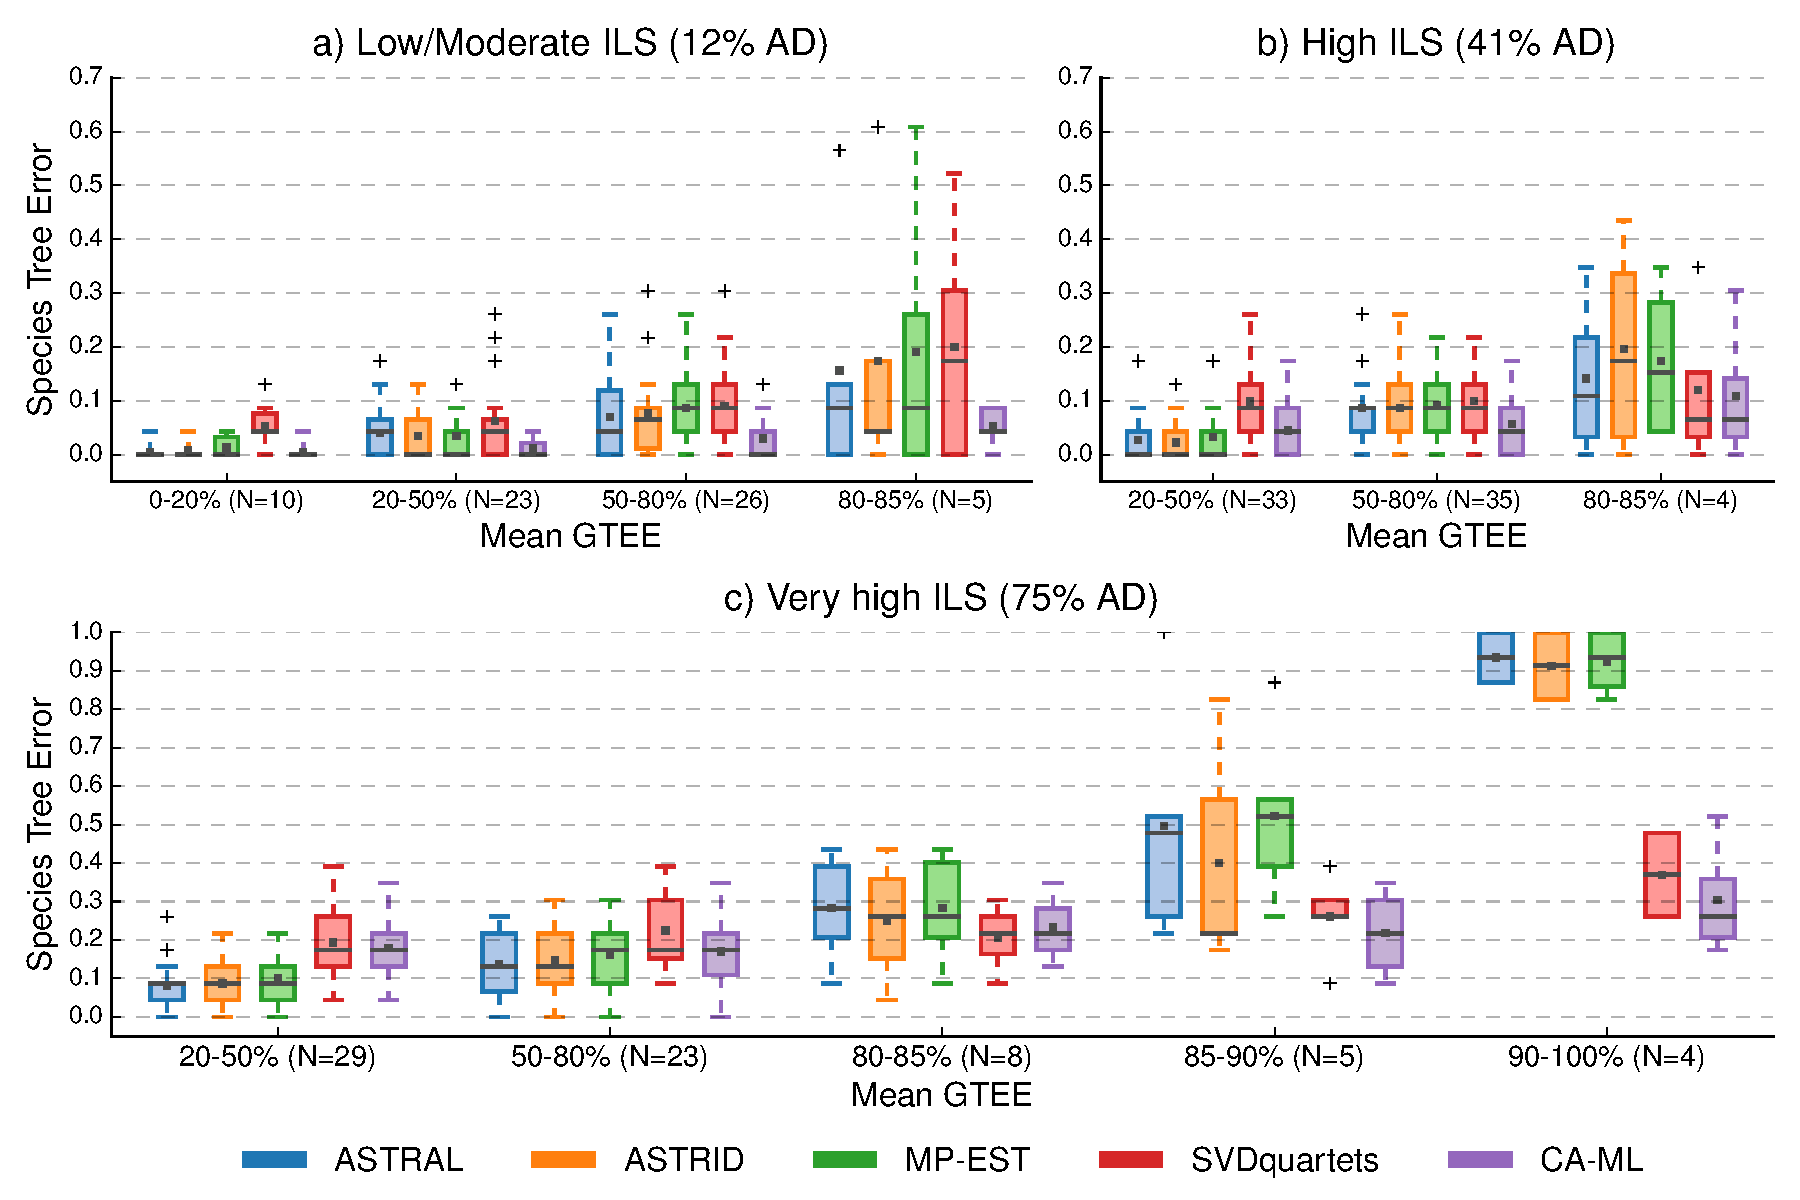
\includegraphics[width=1.0\textwidth]{figures/gene-filtering-fig1.pdf}
\caption{{\bf Impact of GTEE.} The impact of GTEE and ILS on species tree error (RF error rate) is shown for methods: ASTRAL-II (blue), ASTRID (orange), MP-EST (green), SVDquartets (red), and CA-ML using RAxML (purple). 
Subplots a, b, and c show three levels of increasing ILS. 
The mean GTEE range and the number of replicates ($N$) for that model condition are given on the $x$-axis. 
Means and medians are denoted by the gray dot and bar, respectively. Box plots are defined by quartiles, e.g., boxes extend from the first to the third quartiles. 
Greater levels of ILS and/or GTEE increased species tree error rates for all methods, and the relative performance of methods depended on both ILS and GTEE. 
Under low to moderate ILS, CA-ML tended to have better accuracy than the coalescent methods. 
Under higher levels of ILS, summary methods were typically more accurate than CA-ML and SVDquartets except for conditions with high GTEE.}
\label{fig:include-1}
\end{figure}

%\clearpage

\begin{figure}[!h]
\centering
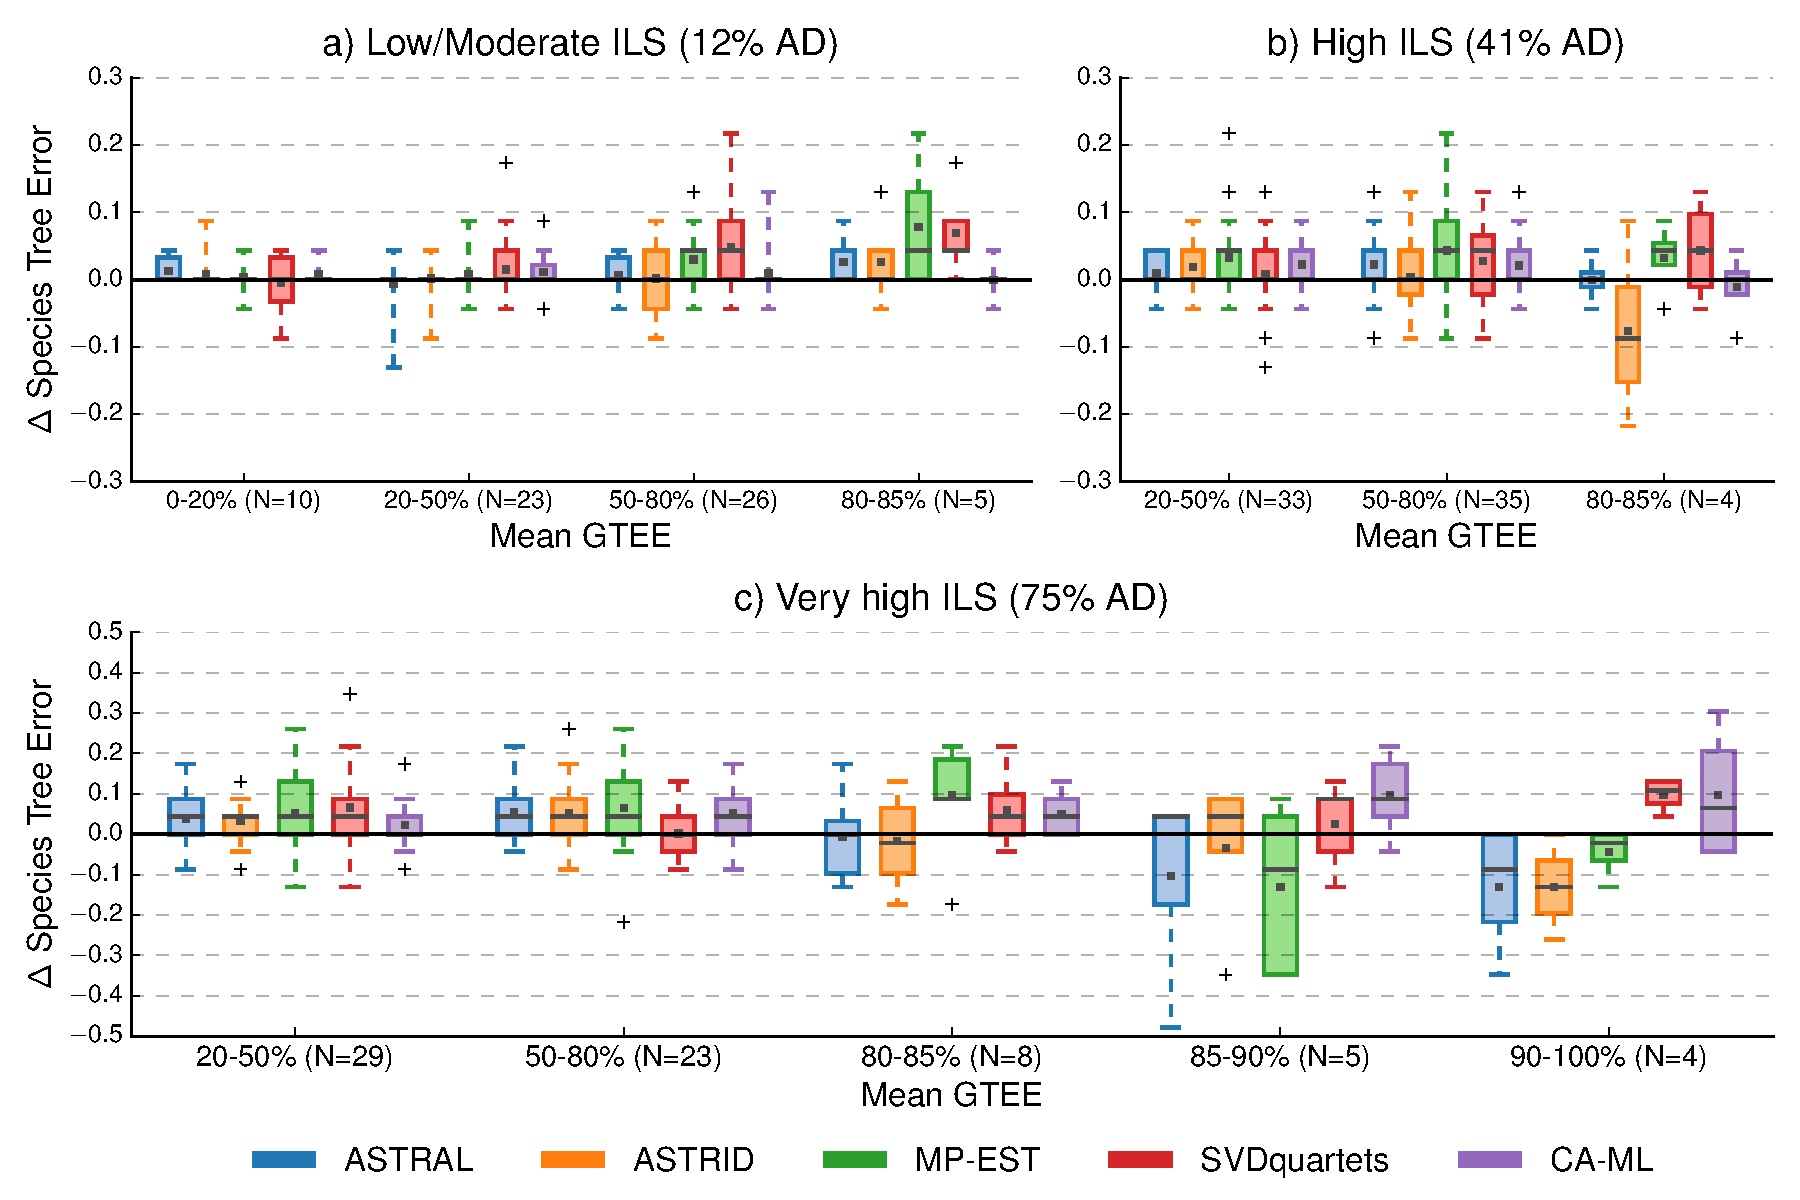
\includegraphics[width=1.0\textwidth]{figures/gene-filtering-fig2.pdf}
\caption{{\bf Impact of missing data.} Differences in species tree error between datasets with no missing data and datasets with approximately 30\% missing data are shown for five methods: ASTRAL-II (blue), ASTRID (orange), MP-EST (green), SVDquartets (red), and CA-ML using RAxML (purple). 
Positive values indicate increases in error, whereas negative values indicate reductions in error. 
Subplots a, b, and c show three levels of increasing ILS. 
The mean GTEE range and the number of replicates ($N$) for that model condition are given on the $x$-axis. 
Means and medians are denoted by the gray dot and bar, respectively. 
Box plots are defined by quartiles, e.g., boxes extend from the first to the third quartiles.}
\label{fig:include-2}
\end{figure}

%\clearpage

\begin{figure}[!h]
\centering
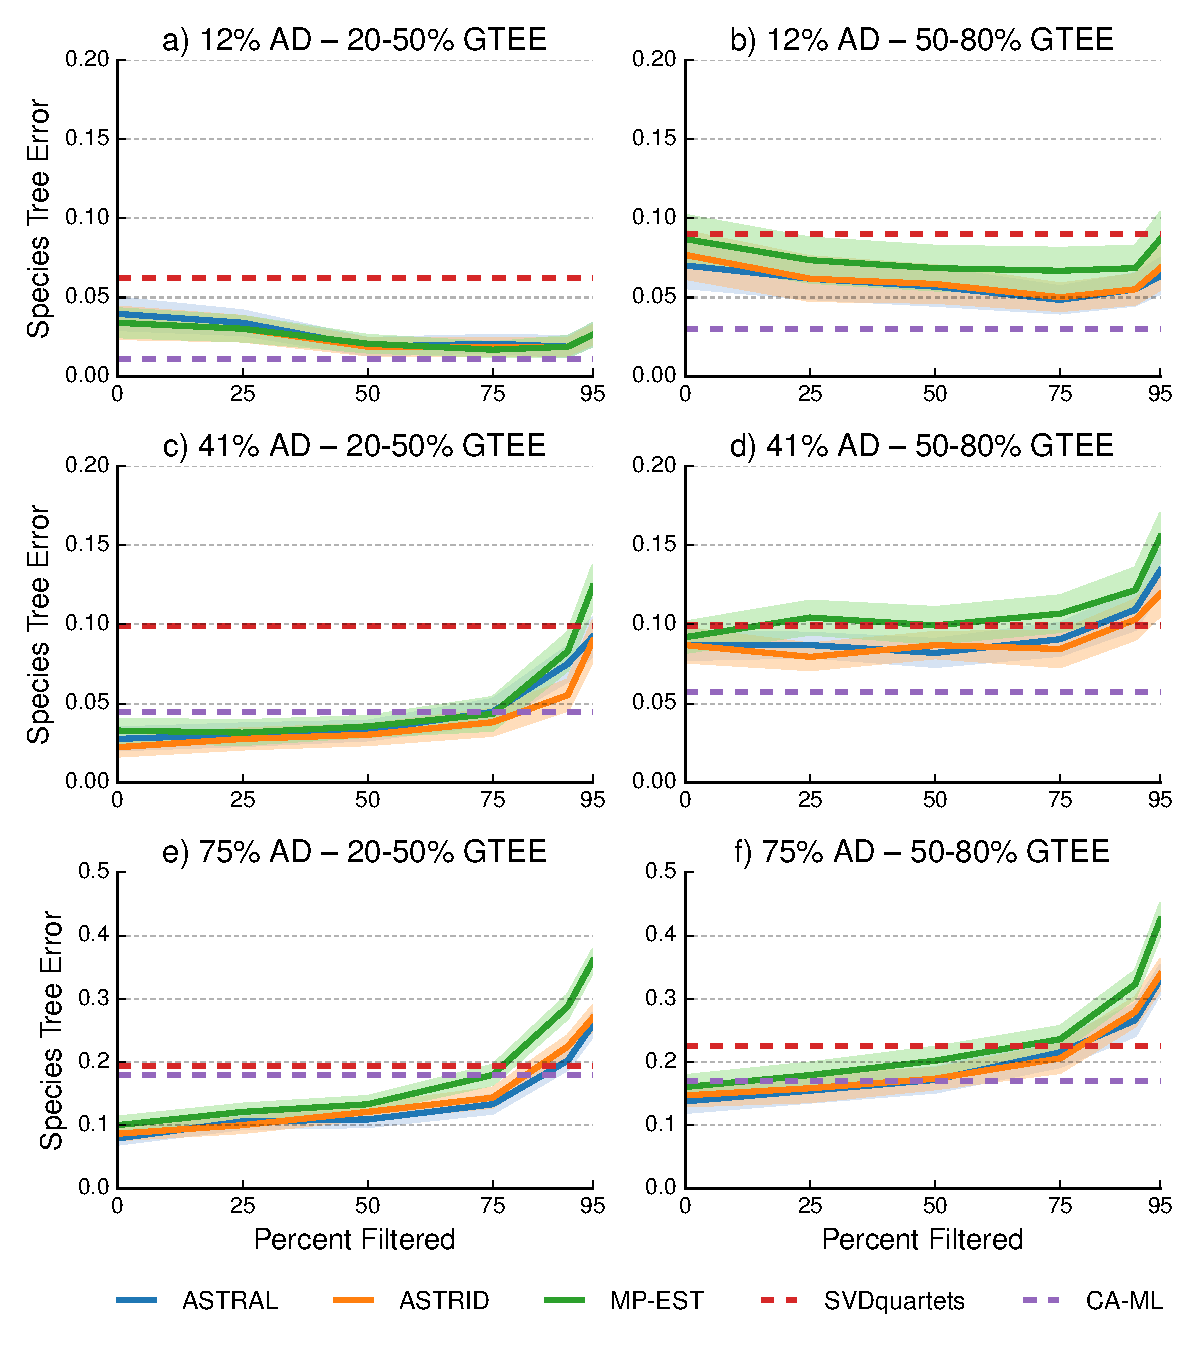
\includegraphics[width=0.80\textwidth]{figures/gene-filtering-fig3.pdf}
\caption{{\bf Impact of filtering based on GTEE.} The impact of filtering genes based on GTEE on species tree error (RF error rate) is shown for three summary methods: ASTRAL-II (solid blue), ASTRID (solid orange), and MP-EST (solid green). 
Genes were filtered by removing the top 25\%, 50\%, 75\%, 90\%, and 95\% of genes with the highest GTEE. 
SVDquartets (dashed red) and unpartitioned concatenation analysis CA-ML using RAxML (dashed purple), are shown without filtering. 
Lines indicate the mean across all replicates, and filled regions indicate the standard error. 
Rows show three levels of ILS, and  columns show two levels of GTEE. 
When ILS was sufficiently low, gene filtering (up to 75\% of genes) increased the accuracy of gene tree summary methods (a-b). When ILS was high to very high, gene filtering had little impact on the accuracy of summary methods or else reduced summary method accuracy (d-f).}
\label{fig:include-3}
\end{figure}

%\clearpage

\begin{figure}[!h]
\centering
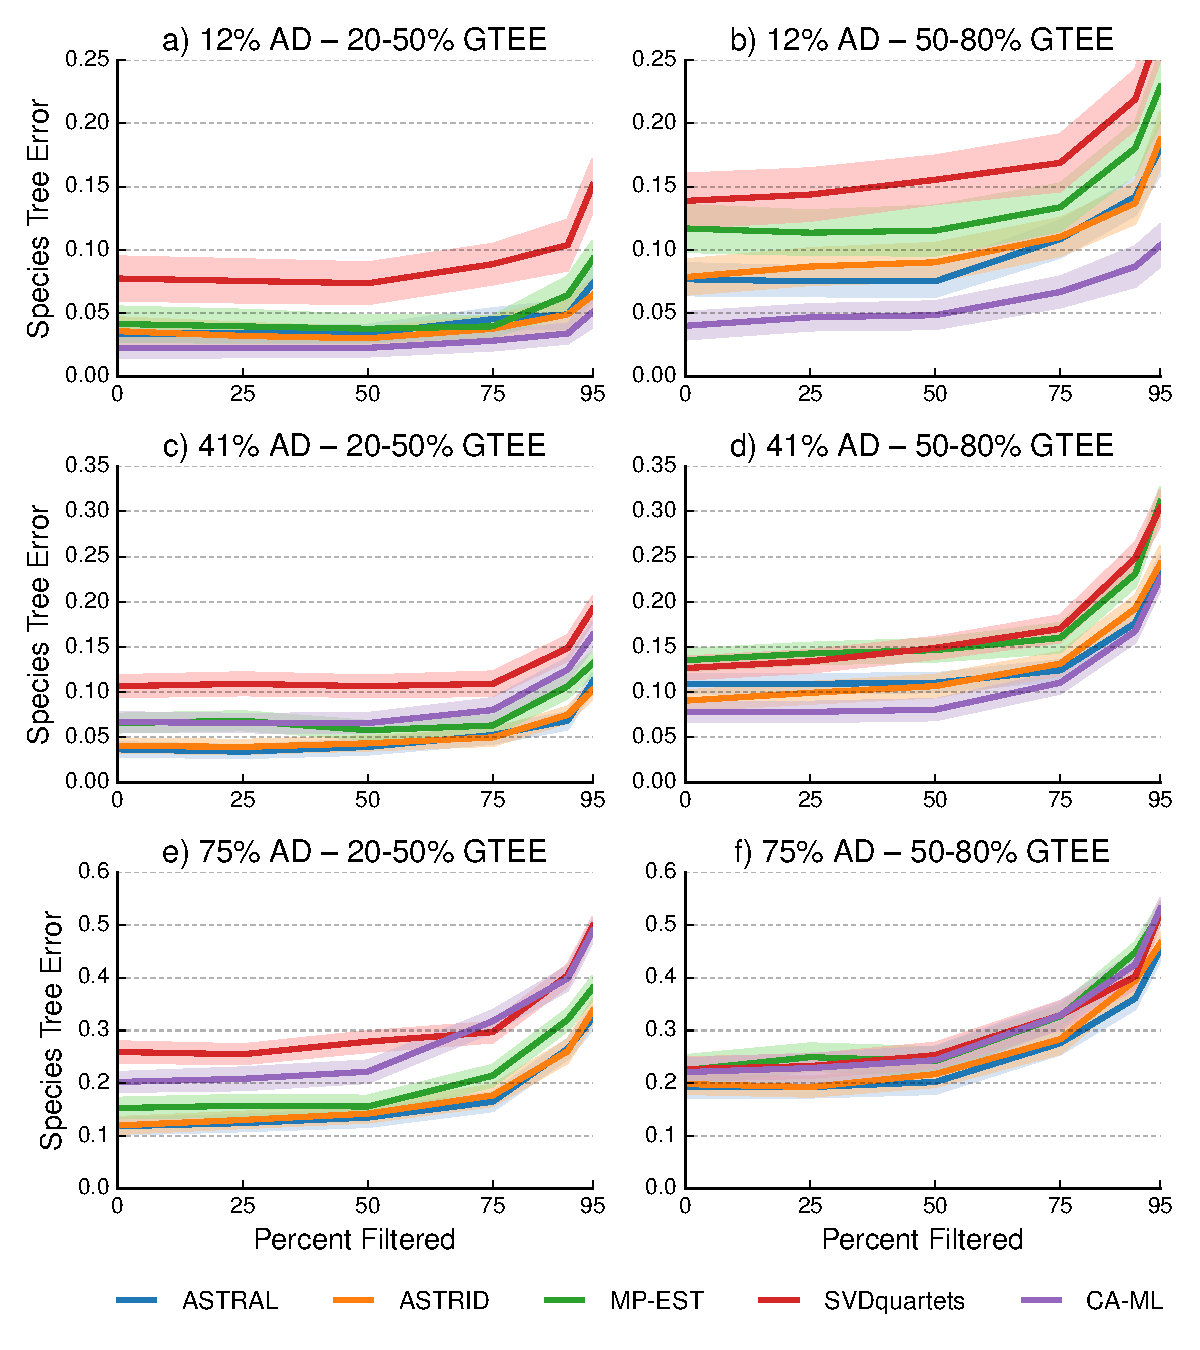
\includegraphics[width=0.80\textwidth]{figures/gene-filtering-fig4.pdf}
\caption{{\bf Impact of filtering based on missing data.} The impact of filtering genes by missing data on species tree error (RF error rate) is shown for five methods: ASTRAL-II (blue), ASTRID (orange), MP-EST (green), SVDquartets (red), and CA-ML using RAxML (purple). 
Genes were filtered by removing the top 25\%, 50\%, 75\%, 90\%, and 95\% of genes with the highest fractions of missing data; this resulted in removing genes missing at least 50\%, 25\%, 10\%, 5\%, and 1\% of species. 
Lines indicate the mean across all replicates, and filled regions indicate the standard error. 
Rows show three levels of increasing ILS, and columns show two levels of GTEE. 
Gene filtering based on missing data was at best neutral but often reduced the accuracy of methods.}
\label{fig:include-4}
\end{figure}

\begin{landscape}
\glsreset{parsimony-informative}
\section{Tables}
\label{sec:include-tables}
This section contains two tables: one presented in Section~\ref{sec:include-intro} Introduction  and one presented in Section~\ref{sec:include-results} Results.

\vspace{12pt}

\begin{table}[!h]
\caption{{\bf Empirical statistics for biological datasets.} 
Means and standard deviations across all genes are reported for the following quantities: MSA length, number of \textit{\gls{parsimony-informative}} sites (sites with at least two character states appearing at least twice), mean bootstrap support, and normalized RF distance between a gene tree and the species tree estimated via CA-ML.
Empirical statistics were computed using the MSAs, bootstrap gene trees, and CA-ML trees provided by these studies. 
In particular, we used the bootstrap gene trees (for each gene) to build a greedy consensus tree and a \textit{\gls{SMC}} tree (all bipartitions in the SMC tree are induced by greater than 50\% of the bootstrapped trees).
The greedy consensus tree was used to compute mean bootstrap support by averaging the bootstrap support values across all branches. 
The SMC tree was used to compute the distance between a gene tree and the species tree computed using CA-ML. 
The distance between the SMC tree and the estimated species tree is separated into False Positive (FP) rate and False Negative (FN) rate. 
FN rate is the fraction of branches in the estimated species tree that are missing from the SMC tree; FP rate is the fraction of branches in the SMC tree that are missing from the CA-ML tree. 
Note that Streicher {\em et al.} \cite{streicher2016how} provided concatenated alignments but not alignments for the individual genes in their Dryad repository, so the mean gene length and the mean number of parsimony informative sites per gene could not be computed.
}\label{tab:include-1}
\centering
\small
\begin{tabular}{l cccc cc cc}
\toprule
& Dataset & Number & Number & Gene & Number of & Mean bootstrap & \multicolumn{2}{c}{SMC versus CA-ML}\\[0.5ex]
Study & type & of species & of gene & length & informative sites & support & FP & FN \\
\midrule
Blom {\em et al.} \cite{blom2017accounting} & exon & 29 & 1361 & 384 $\pm$ 251 & 12 $\pm$ 10 & $0.28 \pm 0.11$ & $0.45 \pm 0.26$ & $0.87 \pm 0.09$ \\[0.5ex]
Hosner {\em et al.} \cite{hosner2016empirical} & \gls{UCE} & 91 & 4817 & 462 $\pm$ 369 & 37 $\pm$ 42 & $0.28 \pm 0.12$ &  $0.37 \pm 0.25$ & $0.83 \pm 0.17$ \\[0.5ex]
Jarvis {\em et al.} \cite{jarvis2014whole} & exon & 48 & 8251 & 1612 $\pm$ 1308 & 453 $\pm$ 418&  $0.26 \pm 0.07$ & $0.22 \pm 0.25$ & $0.85 \pm 0.08$ \\[0.5ex]
Jarvis {\em et al.} \cite{jarvis2014whole} & \gls{intron} & 48 & 2516 & 7654 $\pm$ 8539 & 4315 $\pm$ 4654 & $0.47 \pm 0.12$ & $0.20 \pm 0.13$ & $0.68 \pm 0.09$ \\[0.5ex]
Jarvis {\em et al.} \cite{jarvis2014whole} & UCE & 48 & 3679 & 2509 $\pm$ 164 & 1062 $\pm$ 278 & $0.40 \pm 0.05$ & $0.11 \pm 0.11$ & $0.71 \pm 0.03$ \\[0.5ex]
Streicher {\em et al.} \cite{streicher2016how} & UCE & 29 & 4784 & NA & NA & $0.39 \pm 0.09$ & $0.36 \pm 0.26$ & $0.78 \pm 0.12$ \\[0.5ex]
\bottomrule
\end{tabular}
\end{table}
\fillandplacepagenumber
\end{landscape}

\begin{landscape}
\begin{table}[!h]
\caption{{\bf Proportions of replicates for which filtering based on GTEE increased or decreased the accuracy of ASTRAL-II.} The proportion of replicates for which filtering based on GTEE increased and decreased the accuracy of ASTRAL-II is given on the left and right of the forward slash, respectively. The larger of these two values is in bold. If these two fractions do not sum to one, then the remainder is the proportion of replicates for which filtering did not impact accuracy. The number of replicates as well as the mean ($\pm$ standard deviation) of parsimony informative sites is given for each model condition, specified by the level of ILS and the range of mean GTEE.
}\label{tab:include-2}
\centering
\footnotesize
\begin{tabular}{rc cccccc}
\toprule
Mean & Number of & Number of & \multicolumn{5}{c}{Proportion of replicates affected by filtering (increased / decreased accuracy)} \\[0.5ex]
GTEE & replicates & informative sites & \multicolumn{5}{c}{when the following percentages of genes were removed}\\\cmidrule{4-8}
& & & 25\% & 50\% & 75\% & 90\% & 95\% \\
\midrule
\multicolumn{8}{l}{\em Low/Moderate ILS (12\% AD)}\\[0.5ex]
0-20\%  & 10 & 596 $\pm$ 224  & 0.00 / 0.00 & 0.00 / 0.00 & 0.00 / {\bf 0.10} & 0.00 / 0.00 & 0.00 / {\bf 0.20} \\[0.5ex]
20-50\%  & 23 & 464 $\pm$ 276  & {\bf 0.09} / 0.04 & {\bf 0.26} / 0.00 & {\bf 0.35} / 0.09 & {\bf 0.30} / 0.04 & {\bf 0.26} / 0.13 \\[0.5ex]
50-80\%  & 26 & 63 $\pm$ 14  & {\bf 0.23} / 0.04 & {\bf 0.23} / 0.04 & {\bf 0.31} / 0.12 & {\bf 0.35} / 0.23 & {\bf 0.35} / 0.31 \\[0.5ex]
80-85\%  & 5 & 40 $\pm$ 28  & 0.40 / {\bf 0.60} & 0.40 / 0.40 & 0.40 / {\bf 0.60} & 0.20 / {\bf 0.60} & 0.20 / {\bf 0.80} \\[0.5ex]
85-100\%  & 2 & 5 $\pm$ 3  & {\bf 0.50} / 0.00 & {\bf 1.00} / 0.00 & {\bf 1.00} / 0.00 & {\bf 1.00} / 0.00 & {\bf 1.00} / 0.00 \\[2ex]
\multicolumn{8}{l}{\em High ILS (41\% AD)}\\[0.5ex]
0-20\%  & 2 & 487 $\pm$ 9  & 0.00 / {\bf 0.50} & 0.00 / {\bf 0.50} & 0.00 / {\bf 1.00} & 0.00 / 0.00 & 0.00 / {\bf 0.50} \\[0.5ex]
20-50\%  & 33 & 349 $\pm$ 208  & 0.03 / {\bf 0.09} & 0.15 / {\bf 0.27} & 0.15 / {\bf 0.33} & 0.03 / {\bf 0.55} & 0.03 / {\bf 0.70} \\[0.5ex]
50-80\%  & 35 & 42 $\pm$ 17  & 0.11 / {\bf 0.17} & {\bf 0.26} / 0.17 & 0.26 / {\bf 0.34} & 0.14 / {\bf 0.49} & 0.17 / {\bf 0.60} \\[0.5ex]
80-85\%  & 4 & 22 $\pm$ 10  & {\bf 0.75} / 0.00 & {\bf 0.50} / 0.00 & {\bf 0.25} / 0.00 & 0.25 / 0.25 & 0.25 / {\bf 0.50} \\[0.5ex]
85-100\%  & 1 & 6 $\pm$ 0  & 0.00 / 0.00 & {\bf 1.00} / 0.00 & {\bf 1.00} / 0.00 & {\bf 1.00} / 0.00 & {\bf 1.00} / 0.00 \\[2ex]
\multicolumn{8}{l}{\em Very high ILS (75\% AD)}\\[0.5ex]
0-20\%  & 0 & NA & NA & NA & NA & NA & NA \\[0.5ex]
20-50\%  & 29 & 213 $\pm$ 123  & 0.07 / {\bf 0.45} & 0.07 / {\bf 0.59} & 0.14 / {\bf 0.59} & 0.00 / {\bf 0.93} & 0.00 / {\bf 1.00} \\[0.5ex]
50-80\%  & 23 & 30 $\pm$ 9  & 0.22 / {\bf 0.35} & 0.17 / {\bf 0.61} & 0.09 / {\bf 0.70} & 0.04 / {\bf 0.87} & 0.00 / {\bf 1.00} \\[0.5ex]
80-85\%  & 8 & 17 $\pm$ 10  & {\bf 0.75} / 0.00 & {\bf 0.62} / 0.25 & {\bf 0.62} / 0.25 & {\bf 0.50} / 0.38 & 0.00 / {\bf 0.75} \\[0.5ex]
85-100\%  & 9 & 6 $\pm$ 6  & {\bf 0.56} / 0.00 & {\bf 0.67} / 0.00 & {\bf 0.78} / 0.00 & {\bf 0.78} / 0.11 & {\bf 0.78} / 0.22 \\[0.5ex]
\bottomrule
\end{tabular}
\end{table}
\fillandplacepagenumber
\end{landscape}

\chapter{Divide-and-Conquer Pipelines with NJMerge}
\label{chapter:njmerge}
\textit{This chapter contains material previously published in ``Statistically consistent divide-and-conquer pipelines for phylogeny estimation using NJMerge'' \cite{molloy2019statistically}, which was joint work with T. Warnow.~\emph{NJMerge} is freely available on Github:~\href{https://github.com/ekmolloy/njmerge}{github.com/ekmolloy/njmerge}.
Datasets and software commands necessary to reproduce this study are freely available on the Illinois Data Bank:~\href{https://doi.org/10.13012/B2IDB-1424746_V1}{doi.org/10.13012/B2IDB-1424746\_V1} and \href{https://doi.org/10.13012/B2IDB-0569467_V2}{doi.org/10.13012/B2IDB-0569467\_V2}.~All supplementary tables and figures referenced in this chapter are freely available at {\em Algorithms for Molecular Biology} online:~\href{https://doi.org/10.1186/s13015-019-0151-x}{doi.org/10.1186/s13015-019-0151-x}. 
Note that plots and tables appear at the end of this chapter in Sections~\ref{sec:njmerge-plots} and \ref{sec:njmerge-tables}, respectively.}
\glsreset{DTM}
\glsreset{MSC}
\glsreset{NJMerge}
\glsreset{GTR}
\glsreset{ML}
\glsreset{EPS}
\glsreset{ILS}
\glsreset{AD}
\glsreset{GTEE}
\glsreset{MSA}
\glsreset{RF}
\section{Introduction}
\label{sec:njmerge-introduction}
In Chapter~\ref{chapter:include}, we presented the results of benchmarking species tree estimation methods, including \gls{ASTRAL}, \gls{SVDquartets}, and \gls{CA-ML} using \gls{RAxML}, on datasets with 26 species and $1\,000$ genes.
All three of these methods can be computationally intensive on large datasets with thousands of species and thousands of genes (Section~\ref{sec:background-smethods}), and in this chapter, we address how to scale these methods to larger datasets using divide-and-conquer. 

Divide-and-conquer approaches have been developed in the context of phylogeny estimation, for example the family of disk covering methods \cite{warnow2001absolute, huson1999solving, nakhleh2001designing, lagergren2002combining-dcm}.
Such methods operate by
\begin{enumerate*}[label=(\roman*)]
	\item 
	dividing the species set into overlapping subsets, 	
	\item 
	estimating trees on the subsets, and then
	\item 
	using a \gls{supertree} method to combine the subset trees into a tree on the entire species set.
\end{enumerate*} 
While supertree methods can provide good accuracy (i.e., retain much of the accuracy in the subset trees) under some conditions, many of the most accurate supertree methods are heuristics for NP-hard optimization problems (Section~\ref{sec:background-supertrees}); these methods can be computationally intensive on large datasets.
Note there are other major challenges to building supertrees, for example when there are large terraces of equally optimal solutions \cite{sanderson2011terraces}; see also \cite{brinkmeyer2001polynomial}.

A supertree meta-method, SuperFine \cite{swenson2012superfine}, was developed to address the issue of scalability and was later incorporated into step (iii) of a divide-and-conquer pipeline, DACTAL \cite{nelesen2012dactal}. 
To the best of our knowledge, only one study \cite{bayzid2014disk} has explored using DACTAL for species tree estimation.
Specifically, Bayzid {\em et al.} \cite{bayzid2014disk} used DACTAL to speed-up \gls{MP-EST} on \glspl{multi-locusdataset} with at most 37 species and showed that this approach is \gls{statisticallyconsistent} under the \gls{MSC} model \cite{bayzid2014disk}.
Their code was not publicly available at the time of our study (Md. S. Bayzid, personal communication with T. Warnow).
As recently reviewed by Warnow \cite{warnow2018supertree}, divide-and-conquer continues to be challenging, and yet Bininda-Emonds and many others \cite{bininda2007taxon, bininda2004phylogenetic} have argued that divide-and-conquer is a promising and necessary approach for estimating the Tree of Life.

We propose a new divide-and-conquer approach for scaling \gls{phylogeny} estimation methods to larger datasets that operates by 
\begin{enumerate*}[label=(\roman*)]
	\item 
	dividing the species set into pairwise disjoint subsets, 
	\item 
	estimating a tree on each of subset, and then 
	\item 
	\textit{\glspl{merge}} the subset trees into a phylogeny on the full species set. 
\end{enumerate*}
Note that the term merge refers to building a (refined) \gls{compatibilitysupertree} (Definition~\ref{def:compatibility-supertree}).
While a (refined) compatibility supertree is guaranteed to exist when the subset trees are on pairwise disjoint species sets, the subset tree topologies contain no information about how to perform this merger (Figure~\ref{fig:njmerge-compatibility-supertree}).
Indeed, \textit{\glspl{DTM}} require a set $\mathcal{A}$ of auxiliary data, so DTM methods can be viewed as constrained phylogeny estimation: estimate a phylogeny $T$ from data given in $\mathcal{A}$ subject to the topological constraints implied by the input set $\mathcal{T}$ of subset trees.
This does not require the trees in $\mathcal{T}$ to be \textit{\gls{edgeseparable}} for $T$, meaning that every tree in $\mathcal{T}$ can be obtained from $T$ through a sequence of zero or more edge deletions or conversely that $T$ can be obtained by connecting the trees in $\mathcal{T}$ by edges (Figure \ref{fig:njmerge-compatibility-supertree}).
For example, the \textit{\gls{caterpillartree}} on $\{A,B,C,D,\dots,H\}$ obtained by making a path with the leaves hanging off it in alphabetical order is a compatibility supertree for $\mathcal{T} = \{AC|EG, \; BD|FH\}$, and yet the trees in $\mathcal{T}$ are not edge separable for the caterpillar tree.

\begin{figure}[!h]
\centering
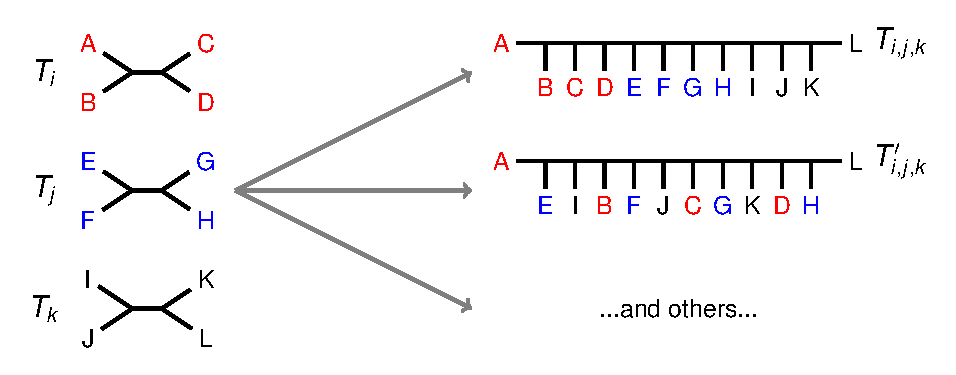
\includegraphics[width=1.0\textwidth]{figures/njmerge-fig1.pdf}
\caption{{\bf Compatibility Supertree Example.} 
Two compatibility supertree for $\mathcal{T} = \{T_i, T_j, T_k \}$ are shown. 
Notably, the trees in $\mathcal{T}$ are \gls{edgeseparable} for $T_{i,j,k}$ but are not edge separable for $T_{i,j,k}'$.
}
\label{fig:njmerge-compatibility-supertree}
\end{figure}

In the remainder of this chapter, we present the first DTM method, \textit{\gls{NJMerge}}.
As we will show, NJMerge runs in polynomial time and enables divide-and-conquer pipelines (for estimating \glspl{genetree} or \glspl{speciestree}) that are provably statistically consistent.
We also present the results of a simulation study evaluating the effectiveness of 
NJMerge for multi-locus species tree estimation.
Our study found that NJMerge improves the running time of ASTRAL-III, SVDquartets, and CA-ML using RAxML without sacrificing accuracy.
Furthermore, NJMerge enabled SVDquartets and RAxML to run on large datasets (e.g., $1\,000$ species and $1\,000$ genes), on which SVDquartets and RAxML would otherwise fail to run when limited to 64 GB of memory.
While NJMerge is not guaranteed to find a compatibility supertree, the failure rate of NJMerge in our experiments was low (less than 1\% of tests), so NJMerge failed on fewer datasets than either ASTRAL-III, SVDquartets, or RAxML when given the same computational resources.
Together, these empirical and theoretical results suggest that NJMerge is a valuable technique for species tree estimation, especially when computational resources are limited.

\section{Approach}
\label{sec:njmerge-approach}
In this section, we present the NJMerge algorithm and then show how it can be used within a divide-and-conquer framework to enable statistically consistent phylogeny estimation pipelines.

\subsection{NJMerge}
NJMerge extends \gls{NJ} by imposing a set of topological constraints on the output tree; therefore, NJMerge has the same input as NJ but additionally requires a set of constraint trees.
\begin{itemize}
	\item \textbf{\gls{NJMergeinput}}: 
	\begin{itemize}
		\item Set $\mathcal{T} = \{T_1, T_2, \dots, T_k\}$ of \gls{unrooted} \glspl{phylogenetictree} such that $S(T_i) \cap S(T_j) = \emptyset$ for all $i \ne j$
		\item Set $\mathcal{A}$ of auxiliary data; specifically
		\begin{itemize}
			\item An $n \times n$ \gls{dissimilaritymatrix} $D$ on label set $S = \cup_{i=1}^k S(T_i)$
		\end{itemize}
	\end{itemize}
	\item \textbf{\gls{NJMergeoutput}}:  A (possibly refined) \gls{compatibilitysupertree} for $\mathcal{T}$ that is \gls{fullyresolved}
\end{itemize}
Because the trees in $\mathcal{T}$ are on pairwise disjoint leaf label sets, we refer to them as being \textit{\gls{leaf-label-disjoint}}.
A compatibility supertree always exists for leaf-label-disjoint trees; however, the objective is to find a tree that is close to the true (but unknown) phylogeny from the set of all compatibility supertrees for $\mathcal{T}$.
NJMerge uses the dissimilarity matrix $D$ to achieve this objective (Figure \ref{fig:njmerge-io}).

The traditional NJ algorithm has an iterative design that builds the tree from the bottom up, producing a \gls{rooted} tree that is then unrooted; this approach is akin to hierarchical clustering.
Initially, there are $n$ leaf labels.
When two leaf labels $x$ and $y$ are selected to be siblings, the pair of leaf leaves is replaced by a single leaf label $z$, which represents a rooted tree on the two leaves.
This reduces the number of leaf labels by one.
This process repeats until there is only one leaf, representing a rooted tree on $n$ leaves; this tree is then unrooted and returned.
Note that at each iteration, NJ makes a siblinghood decision by building a secondary matrix $Q$ from $D$ and simultaneously searching for a minimal element. 
If $Q[i,j]$ is a minimal element of $Q$, leaves $i$ and $j$ are made siblings; see \cite{saitou1987neighbor} for details.

\begin{figure}[!h]
\centering
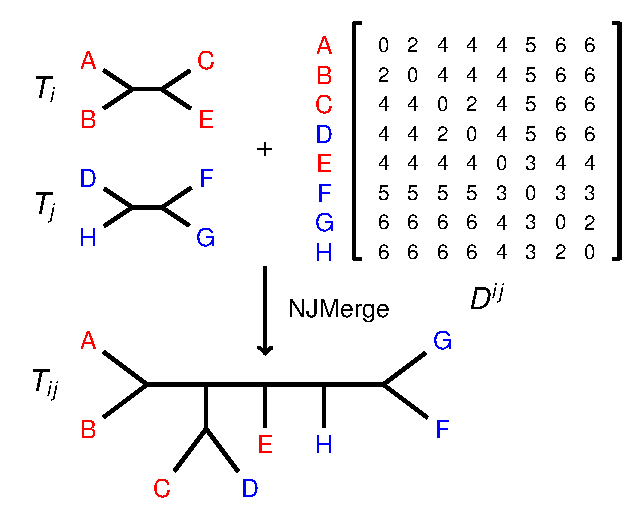
\includegraphics[width=0.75\textwidth]{figures/njmerge-fig2.pdf}
\caption{
{\bf NJMerge Input/Output Example. }
The input to NJMerge is a set $\mathcal{T} = \{ T_i, T_j \}$ of constraint trees and a dissimilarity matrix $D^{ij}$ that is \gls{additive} (Definition~\ref{def:nearly-additive}) for the tree $T$ given by the \gls{newick} string: $(((A,B),(C,D)),E,(F,(G,H)))$ (note that $T$ has the same \gls{topology} as $T_{i,j}$ but swaps leaves $H$ and $F$). 
Traditional NJ applied to $D^{ij}$ returns $T$ (Theorem~\ref{thm:atteson}); however, NJMerge rejects the siblinghood proposal $(G,H)$, because it violates constraint tree $T_j$. 
NJMerge makes $G$ and $F$ siblings, returning tree $T_{i,j}$.
}
\label{fig:njmerge-io}
\end{figure}

NJMerge operates in a similar fashion even using the same formulas as NJ to compute $Q$ and update $D$; however, NJMerge can make different siblinghood decisions than NJ based on the input constraint trees.
After accepting a siblinghood proposal, NJMerge updates $D$ as well as the constraint trees in $\mathcal{T}$.
For example, if $x$ labels a leaf in $T_i$ and $y$ labels a leaf  in $T_j$, then the siblinghood decision $(x,y)$ requires $T_i$ and $T_j$ to be updated by relabeling $x$ in $T_i$ and $y$ in $T_j$ by a new label $z$, which represents the rooted subtree $(x,y)$.
Because siblinghood decisions can result in constraint trees no longer being on pairwise disjoint leaf label sets (Figure \ref{fig:njmerge-join}), they have the potential to make the set of constraint trees incompatible.
Determining whether a set of $k > 2$ unrooted trees is \gls{compatible} (Definition~\ref{def:compatibility-supertree}) is NP-complete  \cite{steel1992complexity,warnow1994tree}, so NJMerge uses a polynomial-time heuristic.

At each iteration, NJMerge sorts the entries of $Q$ from least to greatest and then, based on this ordering, evaluates each siblinghood proposal $(x,y)$ as follows.
\begin{itemize} %[label=(\roman*)]
	\item {\em Test that the proposed siblinghood does not violate the constraint trees.} 
	\begin{itemize}
		\item If $x$ and $y$ both label leaves in some constraint tree $T_i$, check that they label siblings in $T_i$. If not, move to the next siblinghood proposal.
	\end{itemize} 
	\item {\em Use a heuristic to test that the proposed siblinghood does not make the set of constraint trees incompatible.} 
	\begin{itemize}
		\item Update all of the constraint trees as follows. 
		If $x$ and $y$ both label leaves in a constraint tree $T_i$, replace $(x,y)$ by a single leaf labeled $z$.
	If only $x$ (or $y$) are in some constraint $T_i$, then update $T_i$ relabeling $x$ (or $y$) with the new label $z$. 
	\item Use a heuristic to test if $\mathcal{T}$ is compatible. If the test passes, accept the proposal; otherwise, reverse the updates and move to the next proposal.
	\end{itemize}
\end{itemize}
Because a heuristic is used to test compatibility, it is possible for NJMerge to accept a siblinghood proposal that will eventually cause the algorithm to fail when none of the remaining leaves can be joined without violating the compatibility of constraint trees.
Although NJMerge can fail, it is easy to see that when NJMerge returns a tree, it is a compatibility supertree for the input set $\mathcal{T}$ of constraint trees.

\begin{figure}[!h]
\centering
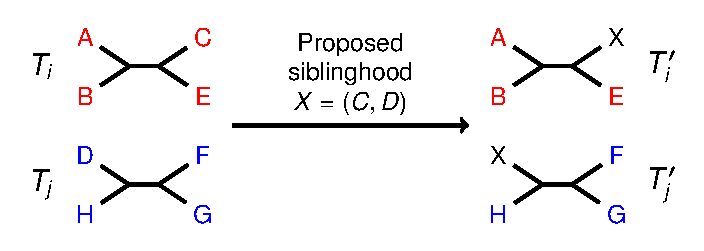
\includegraphics[width=0.8\textwidth]{figures/njmerge-fig3.pdf}
\caption{
{\bf NJMerge Siblinghood Proposal Example. }
In this example, NJMerge evaluates the siblinghood proposal $(C,D)$.
Because $C$ labels a leaf in $T_i$ and $D$ labels a leaf in $T_j$, NJMerge updates the constraint trees $T_i$ and $T_j$ based on the proposed siblinghood, labeling $C$ and $D$ by $X$, which represents the siblinghood $(C,D)$. 
The two updated constraint trees are no longer on disjoint label sets.
}
\label{fig:njmerge-join}
\end{figure}

If a set $\mathcal{T}$ of trees is compatible, then every pair of trees in $\mathcal{T}$ is compatible (the reverse statement does not hold). 
We implemented NJMerge using pairwise compatibility as a heuristic.
It is worth noting that NJMerge was developed as a subroutine of \gls{TreeMerge} (Chapter~\ref{chapter:treemerge}), and in this context, NJMerge is run on $k=2$ constraint trees of bounded size.
In retrospect, it suffices to check only those pairs of constraint trees with leaves labeled by at least one of $x$ and $y$; all other pairs of trees are unchanged by accepting the siblinghood proposal and are pairwise compatible by induction.
After being updated, this subset of constraint trees can be rooted at the edge incident to the leaf labeled $z$, which represents subtree $(x,y)$.
Testing the compatibility of rooted trees can be accomplished in polynomial time \cite{aho1981inferring, deng2018fast}.
Therefore, an alternative heuristic is to test the compatibility of all constraint trees with the new leaf label.

\begin{theorem}
\label{thm:njmerge}
Let $\mathcal{T} = \{T_i \}_{i=1}^k$ be a set of unrooted phylogenetic tree, and let $D$ be an $n \times n$ dissimilarity matrix on label set $S = \bigcup_{i=1}^k S(T_i)$.
Then, NJMerge applied to input $(\mathcal{T}, D)$ fails or returns a (possibly refined) compatibility supertree for $\mathcal{T}$ in $O(n^4k)$ time if using the pairwise compatibility heuristic or in $O(n^4 \log^2{n})$ time if using the alternative heuristic.
\end{theorem}

\begin{proof}
We first prove that if NJMerge completes, then it returns a (possibly refined) compatibility supertree.
At each iteration, NJMerge updates every constraint tree $T_i \in \mathcal{T}$ based on the siblinghood descision.
We use superscript $(w)$ to denote a tree after the $w^{th}$ siblinghood decision, where each leaf representing a rooted subtree is replaced by that subtree.
Initially, $T_i^{(0)}$ is compatible with $T_i$, as no siblinghood decisions have been made (Definition~\ref{def:compatibility}).
Assume that after $w-1$ siblinghood decisions, $T_i^{(w-1)}$ is compatible $T_i$.
At the $w^{th}$ siblinghood decision, there are four cases:
\begin{itemize}
	\item Neither $x$ nor $y$ label leaves in $T_{i}^{(w-1)}$.
	%\begin{itemize}
		%\item  
		NJMerge does nothing. 
	In this case, $T_{i}^{(w)} = T_{i}^{(w-1)}$, so $T_i^{(w)}$ is compatible $T_i$.
	%\end{itemize}
	\item Leaves labeled by $x$ and $y$ are siblings in $T_{i}^{(w-1)}$.
	%\begin{itemize}
		%\item 
		NJMerge replaces $(x,y)$ by a single leaf labeled $z$. 
	In this case, $T_{i}^{(w)} = T_{i}^{(w-1)}$, so $T_i^{(w)}$ is compatible with $T_i$.
	%\end{itemize}
	\item Only $x$ labels a leaf in $T_{i}^{(w-1)}$.
	%\begin{itemize}
		%\item 
		NJMerge relabels $x$ by $z$.
	In this case, $T_{i}^{(w)}$ is $T_{i}^{(w-1)}$ with the subtree represented by $y$ connected to the branch above the subtree represented by $x$, so $T_i^{(w)}$ is compatible with $T_i^{(w-1)}$ and thus is compatible with $T_i$.
	%\end{itemize}
	\item  Only $y$ labels a leaf in $T_{i}^{(w-1)}$. 
	Apply the same argument from above.
\end{itemize}
By induction on the number of siblinghood decisions, $T_i^{(n-1)}$ is compatible with $T_i$ for all $T_i \in \mathcal{T}$.
After $n-1$ iterations, every $T_i \in \mathcal{T}$ is replaced by a single leaf, which represents a rooted tree on $n$ leaves, so $T_1^{(n-1)} = T_2^{(n-1)} = \cdots = T_k^{(n-1)} = T$.
Therefore, the unrooted version of $T$ is a refined compatibility supertree for $\mathcal{T}$.

We now address the worst-case running time of NJMerge (Algorithm~\ref{alg:njmerge} in Section~\ref{sec:njmerge-algorithms}), assuming that $n$ species are divided into $k$ subsets of size $n/k$ for simplicity.
To begin, we compute a vector $\vec{r}$ containing the row sums of $D$ in $O(n^2)$ time. Then, we perform $O(n)$ iterations with each iteration having three steps.
\begin{itemize}
	\item In step 1, we build and sort the $O(n^2)$ entries of $Q$ from least to greatest. Each element of $Q$ can be computed in constant time from $D$ and $\vec{r}$, so this takes $O(n^2\log{n})$ time. % using some reasonable sorting algorithm.
	\item In step 2, we evaluate each siblinghood proposal $z = (x,y)$ in the order suggested by sorting $Q$, breaking on the first siblinghood proposal that passes the heuristic test of compatibility, denoted {\tt IsCompatibleHeuristic} in Algorithm~\ref{alg:heuristic-compatibility} (Section~\ref{sec:njmerge-algorithms}).
	\begin{itemize}
	\item {\em Pairwise compatibility heuristic:} 
	Test the compatibility of all pairs of constraint trees with the new leaf label $z$ are compatible (Algorithm~\ref{alg:pairwise} in Section~\ref{sec:njmerge-algorithms}). 
	This can be achieved by restricting the two trees to their shared leaf label set and then computing their \gls{RF} distance using the linear-time algorithm proposed by Day \cite{day1985optimal}.
	Each of the $k$ trees in $\mathcal{T}$ has at most $n/k$ leaves, so this takes $O(nk)$ time.
	\item {\em Alternative heuristic:} 
	Test the compatibility of all constraint trees with the new leaf label $z$ using the algorithm by Deng and Fern{\'a}ndez-Baca \cite{deng2018fast}, which runs in $O(M \log^2{M})$ time, where $M$ is the total number of edges and nodes in $\mathcal{T}$.
	Each of the $k$ trees in $\mathcal{T}$ has at most $n/k$ leaves, so this takes $O(n \log^2{n})$ time.
	\end{itemize}
	In the best case, the first element passes the heuristic test, and in the worst case, none of the $O(n^2)$ proposals pass the heuristic test (in which case NJMerge fails).
	Therefore, in the worst-case, step 2 requires $O(n^3k)$ time if using the pairwise compatibility heuristic and 
	$O(n^3 \log^2{n})$ time if using the other heuristic.
	\item In step 3, we update $D$ and $\vec{r}$ in $O(n)$ time.
\end{itemize}
In summary, the worst-case running time of NJMerge is $O(n^4k)$ if using the pairwise com-
\clearpage
\noindent patibility heuristic and is $O(n^4 \log^2{n})$ if using the alternative heuristic.
\end{proof}
Note that if the best case always occurs for step 2, then the running time is $O(n^3 \log{n})$; therefore, the running time of NJMerge can vary greatly depending on the input. Although running time improves in this scenario, it means that NJMerge returns the same tree as the traditional NJ algorithm, which is less than ideal, as this means that NJMerge does not improve upon the accuracy of traditional NJ.

%\clearpage

\subsection{Divide-and-Conquer Pipelines for Phylogeny Estimation}
NJMerge can be used in divide-and-conquer pipelines for phylogeny estimation, as shown in Algorithm~\ref{alg:njmerge-divide-and-conquer} and Figure \ref{fig:njmerge-pipeline}. 

\vspace{12pt}

\begin{algorithm}[!h]
\footnotesize
\caption{{\bf Divide-and-Conquer Pipeline using NJMerge.}}
\label{alg:njmerge-divide-and-conquer}
\setstretch{1.15}
\DontPrintSemicolon
\SetAlgoLined
\SetAlgoNoLine
\LinesNumberedHidden
\SetKwFunction{DivideAndConquer}{DivideAndConquer}
\SetKwFunction{NJ}{NJ}
\SetKwFunction{NJMerge}{NJMerge}
\SetKwFunction{Decompose}{Decompose}
\SetKwProg{Pn}{Function}{:}{}
\SetKwInOut{Input}{Input}
\SetKwInOut{Output}{Output} 
\vspace{.1in}
\Input{
\begin{itemize}
	\vspace{-5pt}
	\item[$S$] Set of species labels
	\vspace{-5pt}
	\item[$X$] Dataset for $S$
	\vspace{-5pt}
	\item[$\Phi_D$] Method for estimating distances between pairs of species in $X$
	\vspace{-5pt}
	\item[$\Phi_T$] Method for estimating phylogeny from $X$
	\vspace{-5pt}
	\item[$\Phi_0$] Method for dividing a label set into pairwise disjoint subsets of bounded size %\hspace{36pt}
	given a tree on that label set (e.g., the centroid edge decomposition \cite{mirarab2015pasta})
	\vspace{-5pt}
	\item [$max$] Maximum subset size
\end{itemize}
}
\Output{A (possibly refined) compatibility supertree for $\mathcal{T}$}
\vspace{-4pt}

\hrulefill
 
\Pn{\DivideAndConquer{$X$, $\Phi_T$, $\Phi_D$, $\Phi_0$, $max$}}{
{\bf Step 1:} Estimate distances between all pairs of species.\;
$D \leftarrow \Phi_D(X)$\;
\vspace{10pt}
{\bf Step 2:} Divide the species set into pairwise disjoint subsets.\;
$T_0 \leftarrow \NJ(D)$\;
$\{S_1, S_2, \dots, S_k\} \leftarrow \Phi_0(T_0, max)$\;
\vspace{10pt}
{\bf Step 3:} Estimate a tree on the dataset restricted to each subset of species, producing a set of constraint trees; this can performed in serial or in parallel, depending on the computational resources available.\;
$\mathcal{T} \leftarrow \emptyset$\;
\For{$i \in 1, 2, \dots, k$}{
	$T_i \leftarrow \Phi_T(X |_{S_i})$\;
	$\mathcal{T} \leftarrow \mathcal{T} \cup \{ T_i \}$
}
\vspace{10pt}
{\bf Step 4:} Merge subset trees.\;
$T \leftarrow$ \NJMerge{$\mathcal{T}$, $D$}\;
\vspace{10pt}
\Return{$T$}
	\vspace{6pt}
 }
\end{algorithm}

\begin{figure}[!h]
\centering
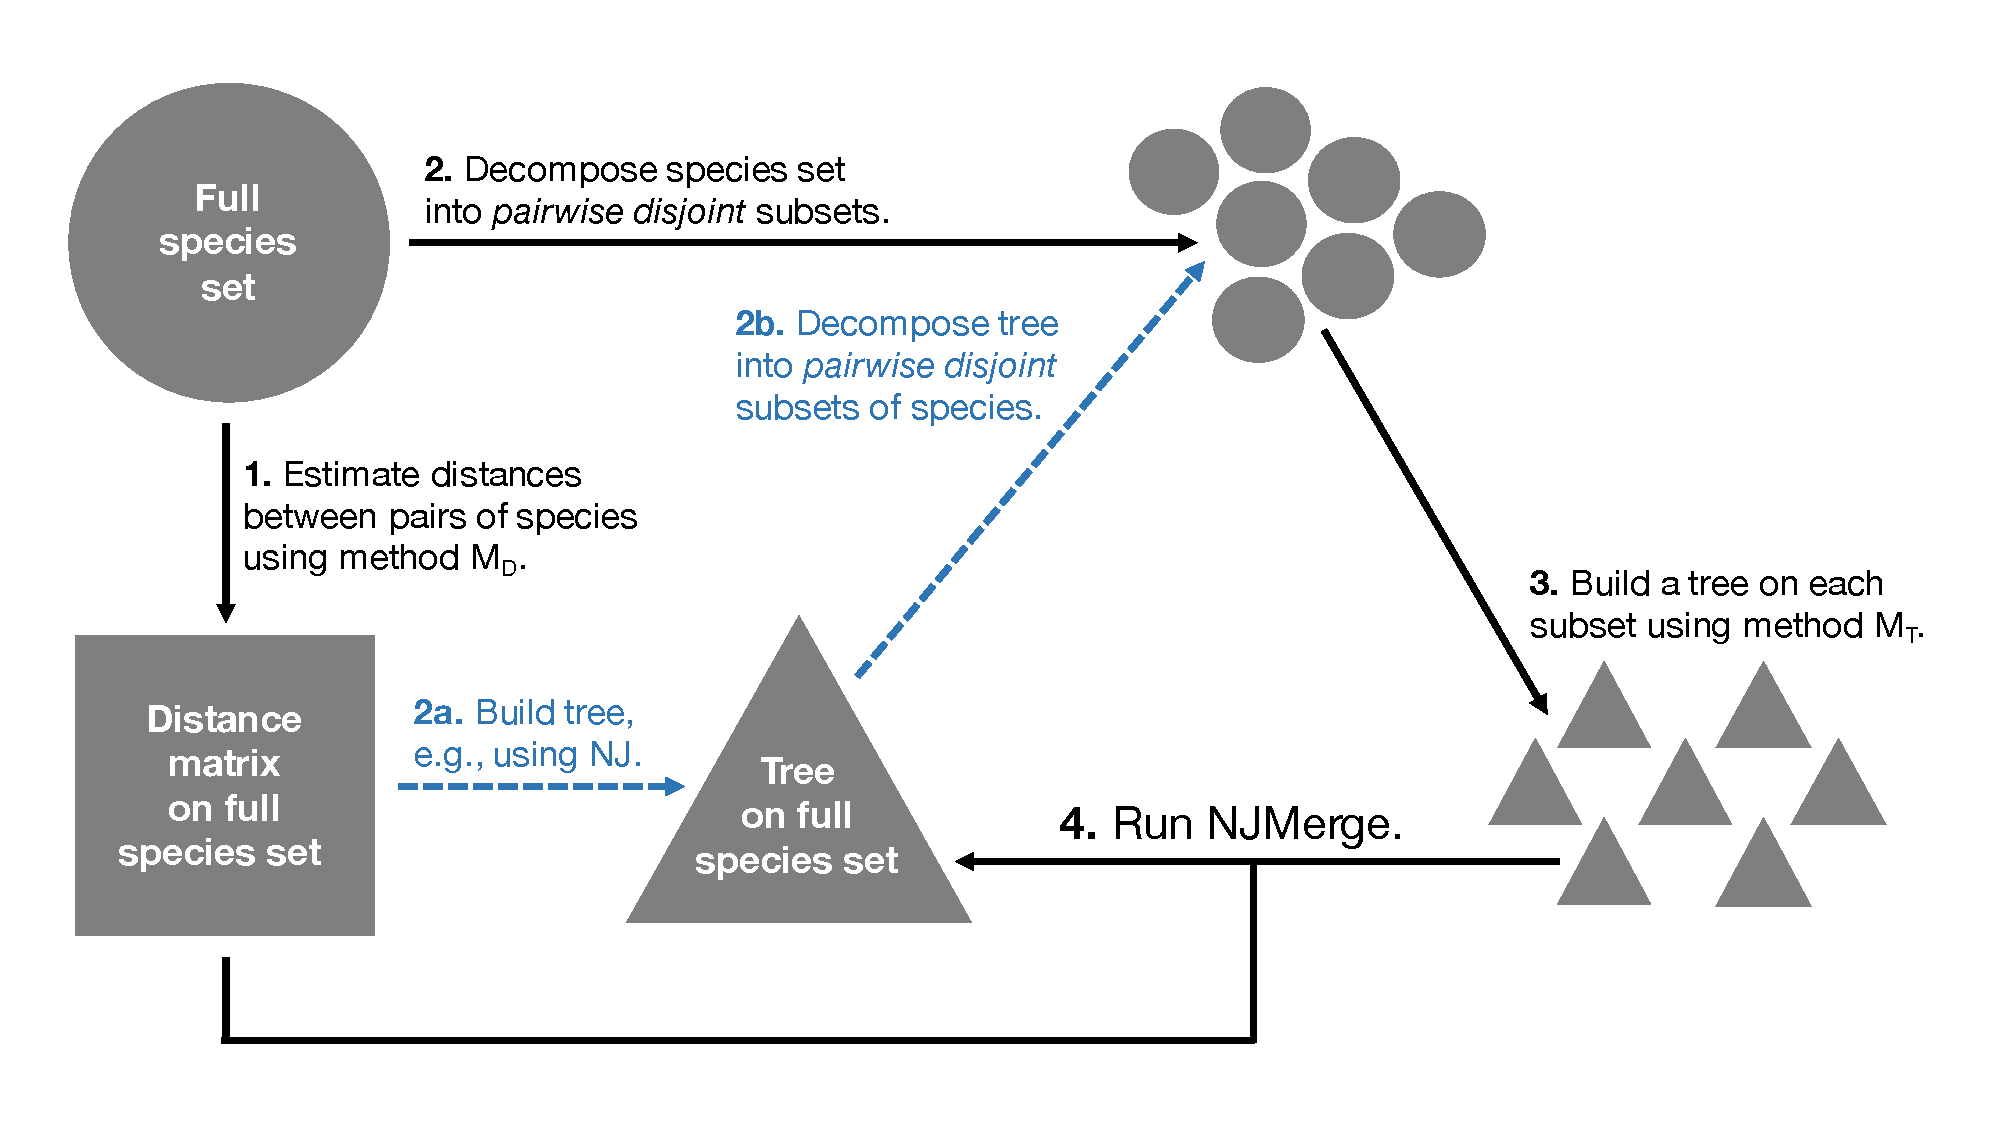
\includegraphics[width=1.0\textwidth]{figures/njmerge-fig4.pdf}
\caption{{\bf Divide-and-Conquer Pipeline using NJMerge.} Circles are sets of (species) labels, squares are dissimilarity matrices, and  triangles are phylogenetic trees. 
Note that henceforth $M_D$ (in step 1) is referred to as $\Phi_D$ and $M_T$ (in step 3) is referred to as $\Phi_T$.}
\label{fig:njmerge-pipeline}
\end{figure}

\subsection{Statistical Consistency}
Algorithm~\ref{alg:njmerge-divide-and-conquer} shows that a user must select a method for estimating a dissimilarity matrix $\Phi_D$ (step 1), a method $\Phi_0$ for dividing the leaf labels of a tree into pairwise disjoint subsets (step 2), a maximum subset size $max$ (step 2),  and a method $\Phi_T$ for estimating subset trees (step 3).
Therefore, users can select methods $\Phi_D$ and $\Phi_T$ to be appropriate for gene tree estimation or species tree estimation (note that the user also should select $max$ to be appropriate given these methods and the computational resources that they can access).
We prove that with the proper choices of $\Phi_D$ and $\Phi_T$ divide-and-conquer pipelines using NJMerge are statistically consistent under the \gls{GTR} model of DNA evolution and under the MSC model.
These results follow from Theorem \ref{thm:njmerge-correct}.

\begin{theorem}
\label{thm:njmerge-correct}
Let $\mathcal{T} = \{T_1, T_2, \dots, T_k \}$ be a set of unrooted phylogenetic trees, and let $D$ be an $n \times n$ dissimilarity matrix on label set $S = \bigcup_{i=1}^k S(T_i)$, and let $T^*$ be an unrooted, fully resolved tree on label set $S$.
Suppose that $D$ is a \gls{nearlyadditive} matrix for $T^*$ (Definition~\ref{def:nearly-additive}) and that $T^*$ is compatible with $T_i$ for all $i \in \{1, \dots, k\}$ (Definition~\ref{def:compatibility}).
Then, NJMerge applied to input $(\mathcal{T}, D)$ returns $T^*$.
\end{theorem}
\begin{proof}
NJ applied to a nearly additive dissimilarity matrix for $T^*$ will return $T^*$ (Theorem~\ref{thm:atteson}).
Because $T^*$ is compatible with every tree in $\mathcal{T}$, the siblinghood proposals suggested by NJ will never violate the trees in $\mathcal{T}$ or the (heuristic test of the) compatibility of $\mathcal{T}$.
It follows that NJMerge applied to $(\mathcal{T}, D)$ will return the same output as NJ applied to $D$, which is $T^*$.
\end{proof}

We now define statistical consistency in the context of gene tree estimation (Definition \ref{def:sc-gene}) and show that NJMerge can be used to create statistically consistent divide-and-conquer pipelines for gene tree estimation (Corollary \ref{cor:sc-gene}).

\glsreset{statisticallyconsistent}

\begin{definition}[Statistical Consistency under GTR model]
\label{def:sc-gene}
Let $(T,\Theta)$ be a GTR model tree with topology $T$ and numerical parameters $\Theta$.
A method $M$ for constructing gene trees from DNA sequences is statistically consistent under the GTR model if, for all $\epsilon > 0$, there exists a constant $ l > 0$ such that, when given at least $l$ sites generated independently from the GTR model tree, $M$ returns the unrooted version of $T$ with probability at least $1 - \epsilon$.
\end{definition}

\begin{corollary}
\label{cor:sc-gene}
NJMerge can be used in a gene tree estimation pipeline that is statistically consistent under the GTR model. 
\end{corollary}
\begin{proof}
Let $(T^*, \Theta)$ be a GTR model tree, let $\Phi_D$ be a method for calculating distances between pairs of DNA sequences, and let $\Phi_T$ be a method for constructing trees from site patterns (DNA sequences).
Suppose that 
\begin{itemize}
	\item the divide-and-conquer pipeline produces $k$ pairwise disjoint subsets of DNA sequences labeled by the set $S$
	\item method $\Phi_D$ is statistically consistent under the GTR model, for example  the \gls{log-detdistance} \cite{steel1994recovering})
	\item method $\Phi_T$ is statistically consistent under the GTR model, for example a \gls{ML} method \cite{truszkowski2016maximum}
\end{itemize}
Now let $\epsilon > 0$, and select $\epsilon_D, \epsilon_T > 0$ such that $\epsilon_D + k \epsilon_T < \epsilon$.
By Definition \ref{def:sc-gene}, there exists a constant $l_D$ such that NJ applied to matrix $D$ computed from DNA sequences with at least $l_D$ sites returns $T^*$ with probability at least $1 - \epsilon_D$, and there exists a constant $l_T$ such that $\Phi_T$ given DNA sequences with at least $l_T$ sites returns $T^*$ with probability at least $1 - \epsilon_T$.
If a phylogenetic distance matrix $D$ is calculated using $\Phi_D$ and a set of $k$ phylogenetic (constraint) trees $\mathcal{T}$ are constructed using $\Phi_T$, given DNA sequences with at least $\max\{l_D, l_T\}$ sites, then the probability that NJ applied to $D$ returns $T^*$ and that $\Phi_T$ returns a tree that agrees with $T^*$ for all $k$ constraint trees in $\mathcal{T}$ is at least $1 - \epsilon$, as
\begin{align}
	(1 - \epsilon_D) (1 - \epsilon_T)^k &\ge (1 - \epsilon_D) (1 - k \epsilon_T) \quad \text{by Bernoulli's Inequality \cite{bernoulli}}  \\
	&= 1 - \epsilon_D - k \epsilon_T + k \epsilon_D \epsilon_T \nonumber \\
	&> 1 - (\epsilon_D + k \epsilon_T) > 1 - \epsilon \nonumber
\end{align}
Then, by Theorem \ref{thm:njmerge-correct}, NJMerge applied to the input $(\mathcal{T}, D)$ will return the $T^*$ with probability at least $1 - \epsilon$, and by Definition \ref{def:sc-gene}, NJMerge is statistically consistent under the GTR model.
\end{proof}

Finally, we define statistical consistency in the context of species tree estimation (Definition \ref{cor:sc-species}) and show that NJMerge can be used to create statistically consistent divide-and-conquer pipelines for species estimation (Corollary \ref{cor:sc-species}).

\glsreset{statisticallyconsistent}

\begin{definition}[Statistical Consistency under MSC model]
\label{def:sc-species}
Let $(T,\Theta)$ be an MSC model tree with topology $T$ and numerical parameters $\Theta$.
A method $M$ for constructing species trees from true gene trees is statistically consistent under the MSC model if, for all $\epsilon > 0$, there exists a constant $m > 0$ such that, given at least $m$ gene trees generated independently from the MSC model tree, $M$ returns $T$ with probability at least $1 - \epsilon$.
\end{definition}

\begin{corollary}
\label{cor:sc-species}
NJMerge can be used in a species tree estimation pipeline that is statistically consistent under the MSC model.
\end{corollary}
\begin{proof}
This proof is similar to Corollary \ref{cor:sc-gene} except that we must make choices appropriate for species trees estimation.
Therefore, we would suppose that 
\begin{itemize}
	\item the divide-and-conquer pipeline produces $k$ pairwise disjoint subsets of species labeled by the set $S$
	\item method $\Phi_D$ is statistically consistent under the MSC model, for example the \gls{AGID} \cite{allman2018species-internode} 
	\item method $\Phi_T$ is statistically consistent under the MSC model, for example  ASTRAL \cite{mirarab2014astral}
\end{itemize}
and then, letting $\epsilon > 0$, we would select $\epsilon_D, \epsilon_T > 0$ such that $\epsilon_D + k \epsilon_T < \epsilon$ and proceed in a fashion similar to Corollary \ref{cor:sc-gene}.
\end{proof}

Note that the above proof easily could be extended to the \gls{MSC+GTR} model for \glspl{site-basedmethod} that take the \gls{concatenatedalignment} as input.

Lastly, because distance estimation (for $D$) and phylogeny estimation (for $\mathcal{T}$) are both performed using statistically consistent methods, this begs the question: why not just run NJ instead of NJMerge?
The major take-away is that data are neither infinite nor error-free in practice, so two statistically consistent methods can perform very differently (in terms of accuracy) on the same dataset.

\section{Performance Study}
\label{sec:njmerge-study}
We present results of using NJMerge to estimate species trees on large multi-locus datasets simulated using the protocol presented in \cite{mirarab2015astral2}.
Our simulation produced four model conditions, described by two numbers of species (100 and $1\,000$) and two levels of ILS (low/moderate and very high), each with 20 replicate datasets.
Datasets included both \gls{exon}-like sequences and \gls{intron}-like sequences with exons characterized by slower rates of evolution across sites (less phylogenetic signal) and introns characterized by faster rates of evolution across sites (greater phylogenetic signal).
The 100-species datasets were analyzed using 25, 100, and $1\,000$ genes, and the $1\,000$-species datasets were analyzed using $1\,000$ genes; note that exons and introns were always analyzed separately.
For each of these 320 datasets, we estimated dissimilarity matrices using two different methods and constraint trees using four different methods.
This provided $2\,560$ different tests on which to evaluate NJMerge.
NJMerge failed on 11/$2\,560$ tests, so the failure rate in our experiments was less than 1\% (although these tests are not independent).
Species tree estimation methods were evaluated in terms of running time and species tree error, as measured by the \gls{RFerrorrate} (Equation~\ref{eq:rf-error}).

\subsection{Simulated Datasets}
\label{sec:njmerge-datasets}
\paragraph{Species trees and gene trees:} 
Datasets, each with a true species tree and 2000 true gene trees, were simulated under the MSC model using \gls{SimPhy} version 1.0.2.
All model conditions had deep speciation (towards the root) and 20 replicate datasets.
By holding the \gls{EPS} constant (200K) and varying the species tree height (in generations), model conditions with different levels of \gls{ILS} were generated.
For species tree heights of 10M and 500K generations, the \gls{AD} was 8--10\% and 68--69\% respectively.
Thus, we referred to these levels of ILS as ``low/moderate'' and ``very high,'' respectively.

\paragraph{DNA (gene) sequence data:} 
DNA sequences were simulated for each true gene tree using \gls{INDELible} version 1.03 \cite{fletcher2009indelible} under the \gls{GTR+GAMMA} model.
For each gene, the parameters for the GTR+GAMMA model ($\vec{\pi}$, $Q$, and $\alpha$) were drawn from distributions based on estimates of these parameters from the Avian Phylogenomics Dataset \cite{jarvis2014whole}.
Distributions were fitted for exons and introns, separately (Supplementary Table S1), so for each dataset (with 2000 genes), $1\,000$ gene sequences were simulated with parameters drawn from the exon distributions, and $1\,000$ gene sequences were simulated with parameters drawn from the intron distributions.
Sequence lengths were also drawn from a distribution (varying from 300 to $1\,500$ bp).
DNA sequences were simulated without insertions or deletions, so \gls{MSA} estimation was not necessary.

\paragraph{Estimated gene trees:} 
ML gene trees were estimated using \gls{FastTree-2} version 2.1.10 under the \gls{GTR+CAT} model. 
GTEE was computed as the \gls{normalizedsymmetricdifference} between true and estimated gene trees (Equation~\ref{eq:nsd}), averaged across all gene trees. 
Across all model conditions datasets, the \gls{GTEE}, averaged across all replicates, ranged from 26\% to 51\% for introns and 38\% to 64\% for exons and thus was higher for exon datasets (Supplementary Table S2).

\subsection{Species Tree Estimation}
For each model condition (characterized by number of species and level of ILS), species tree estimation methods were run either given the exon-like genes or the intron-like genes as input. 
Species trees were estimated on 25, 100, or $1\,000$ genes for the 100-species species and $1\,000$ genes for the $1\,000$-species datasets using three different methods: ASTRAL-III (as implemented in version 5.6.1), SVDquartets (as implemented in \gls{PAUP*} version 4a161), and CA-ML under the \gls{GTR+GAMMA} model (as implemented in RAxML version 8.2.12 with pthreads and SSE3).

\subsection{Divide-and-conquer pipeline using NJMerge}
\paragraph{Distance matrices:} Distance matrices were created using two different approaches.
\begin{itemize}
	\item $D_{AGID}$ denotes the AGID matrix computed from estimated gene trees using \gls{ASTRID} version 1.1.
	\item $D_{LD}$ denotes the log-det distance matrix computed from concatenated alignment using PAUP* version 4a163.
\end{itemize}

\paragraph{Subset decomposition:}  
We decomposed the species set into subsets as indicated by the blue dashed arrows in Figure \ref{fig:njmerge-pipeline}.
First, a starting tree was built by running NJ (as implemented in \gls{FastME} version 2.1.5) on the estimated dissimilarity matrix and then used to define pairwise disjoint subsets of species.
Essentially, the set of species was divided into subsets by repeatedly deleting centroid edges (edges whose deletions divide the leaf set roughly in half) until the resulting subsets are smaller than the predetermined maximum size; see the \textit{\gls{centroidedgedecomposition}} described in PASTA \cite{mirarab2015pasta}.
Datasets with 100 species were decomposed into four to six subsets with a maximum subset size of 30 species, and datasets with $1\,000$ species were decomposed into 10--15 subsets with a maximum subset size of 120 species.

\paragraph{Constraint trees:}
Constraint trees were created using four different approaches.
\begin{itemize}
     \item $\mathcal{T}_{true}$ denotes constraint trees computed by restricting the true species tree to each subset of species.
	\item $\mathcal{T}_{AST}$ denotes constraint trees estimated by running ASTRAL-III on each subset, i.e., on the estimated gene trees restricted to each subset of species.
	\item $\mathcal{T}_{SVD}$  denotes constraint trees estimated by running SVDquartets on each subset, i.e., on the concatenated alignment restricted to each subset of species.
	\item $\mathcal{T}_{RAX}$  denotes constraint trees estimated by running RAxML on each subset, i.e., on the concatenated alignment restricted to each subset of species.
\end{itemize}

\paragraph*{Notation:}
We often specify the inputs to NJ and NJMerge using the following notation: NJ($D$) and NJMerge($\mathcal{T}$, $D$). For example, NJMerge($\mathcal{T}_{RAX}$, $D_{LD}$) refers to NJMerge given the RAxML constraint trees and the log-det distance matrix as input, whereas NJMerge($\mathcal{T}_{RAX}$, $D$) refers to NJMerge given the RAxML constraint trees and {\em either} the AGID matrix {\em or} the log-det distance matrix as input.

\subsection{Computational Experiments and Running Time Evaluation}
\label{sec:njmerge-comp}
All computational experiments were run on the Blue Waters supercomputer, specifically the XE6 dual-socket nodes with 64 GB of physical memory and two AMD Interlagos model 6276 CPU processors (i.e., one per socket each with 8 floating-point cores).
All methods were given access to 16 threads with 1 thread per bulldozer (floating-point) core.
SVDquartets and RAxML were explicitly run with 16 threads; however, ASTRAL-III and NJMerge were not implemented with multi-threading at the time of this study.
All methods were restricted to a maximum wall-clock time of 48 hours.

Running time was measured as the wall-clock time recorded in seconds.
For ASTRAL, SVDquartets, and RAxML, timing data was recorded for running the method on the full dataset as well as for running the method on subsets of the dataset to produce constraint trees for NJMerge.
RAxML did not complete within the maximum wall-clock time of 48 hours on datasets with $1\,000$ species, so we used the last checkpoint file to evaluate species tree estimation error and running time (i.e., running time was the time between the info file being written and the last checkpoint file being written).

We computed the total running time of the NJMerge pipeline by combining the timing data for estimating the dissimilarity matrix, estimating the subset trees, and running NJMerge; see Supplementary Tables S9 and S10 for the average time required for each of these steps.
If a user only had access to one compute node, subset trees would need to be estimated in serial, so the running time of the NJMerge pipeline would be
 \begin{equation}\label{eq:serial}
time\big(\Phi_D(X)\big) + \sum_{T \in \mathcal{T}} time\big(\Phi_T(X|_{S(T)})\big) + time\big(NJMerge(\mathcal{T}, D)\big)
\end{equation}
using the notation defined in Algorithm~\ref{alg:njmerge-divide-and-conquer}.
Note that Equation~\ref{eq:serial} does not include the timing data for estimating the starting tree, as this took less than a minute even for datasets with $1\,000$ species.
Finally, if given access to multiple compute nodes (at least six nodes for the 100-species datasets and at least 15 nodes for the $1\,000$-species datasets), the subset trees could be estimated in an embarrassingly parallel fashion.
In this case, the running time of the NJMerge pipeline would be
 \begin{equation}
 \label{eq:parallel}
time\big(\Phi_D(X)\big) + \max_{T \in \mathcal{T}} \{ time\big(\Phi_T(X|_{S(T)})\big) \} + time\big(NJMerge(\mathcal{T}, D)\big)
\end{equation}
Results computed using Equation~\ref{eq:parallel} are provided in \cite{molloy2018njmerge}.

It is worth noting that running ASTRAL-III and computing the AGID matrix require gene trees to be estimated.
Using the same experimental set-up (a single Blue Waters compute node with 64 GB of memory and 16 floating-point cores), FastTree-2 took on average $18 \pm 2$ minutes to estimate $1\,000$ gene trees for datasets with 100 species and on average $217 \pm 20$ minutes to estimate $1\,000$ gene trees for datasets with $1\,000$ species (Supplementary Tables S4 and S5).
The amount of time for gene tree estimation can vary greatly, depending on the method used and the analysis performed.
We did not include the time to estimate gene trees in the reported running times.

\section{Results}
\label{sec:njmerge-results}
Pipelines using NJMerge can be viewed in two different ways:  
%\begin{enumerate*}[label=(\roman*)]
	%\item
	(i) as techniques for potentially improving the accuracy of NJ (hopefully without a large increase in running time) or  
	%\item 
	(ii) as techniques for potentially improving the scalability of the method used to estimate constraint trees (hopefully without sacrificing accuracy).
%\end{enumerate*}
For the former, we would expect NJMerge to improve the accuracy of traditional NJ whenever distance-based species tree estimation is less accurate than other methods (which can used to estimate constraint trees).
For the latter, we would expect NJMerge to improve the running time of methods (used to estimate constraint trees) whenever these methods are more computationally intensive than distance-based methods (which is often the case).

We compared the accuracy of the NJMerge pipeline to traditional NJ, and we also compared the accuracy and  running time of the NJMerge pipeline to running $\Phi_T$ on the full dataset, where $\Phi_T$ is the method used to estimate the constraint trees for NJMerge.
Results for intron-like datasets are provided below, and results for exon-like datasets are provided in the Supplementary Materials.
Unless otherwise noted, results were similar for both sequence types; however, species trees estimated on the exon datasets had slightly higher error rates than those estimated on the intron datasets.
This is expected, as the exons had slower rates of evolution (and thus less phylogenetic signal) than the introns.

\subsection{How do pipelines using NJMerge compare to NJ?}
In this section, we report on the effectiveness of using NJMerge as compared to traditional NJ in terms of species tree accuracy.

\paragraph{Impact of estimated dissimilarity matrix:}
In this section, we compare traditional NJ to the NJMerge pipeline, both given distance matrices estimated from 100-species datasets with varying numbers of genes (Figure \ref{fig:true-intron} and Supplementary Figure S1).
Because the accuracy of NJMerge also depends on the amount of error in the input constraint trees, we studied the ideal case, giving NJMerge true constraint trees (i.e., constraint trees that agreed with the true species tree).
We found that NJMerge($\mathcal{T}_{true}$, $D$) was more accurate than NJ($D$) for all model conditions and that the difference in error was especially large when the number of genes was small and the level of ILS was very high; for example, the difference in mean error was greater than 15\% when matrices were estimated from 25 introns but was closer to 5\% when matrices were estimated from $1\,000$ introns.
A similar trend was observed for matrices computed using the log-det distance.
Interestingly, both NJ($D$) and NJMerge($\mathcal{T}_{true}$, $D$) were more accurate when given the AGID matrix rather than the log-det distance matrix as input even when ILS was low/moderate.
In summary, NJMerge($\mathcal{T}_{true}$, $D$) was always more accurate than NJ($D$), but the improvement in accuracy was greater under challenging model conditions, suggesting that NJMerge($\mathcal{T}_{true}$, $D$) is more robust to error in the estimated dissimilarity matrix than NJ($D$).

\paragraph{Impact of estimated constraint trees:}
In this section, we compare traditional NJ to the NJMerge pipeline given estimated constraint trees on datasets with $1\,000 $species and $1\,000$ genes (Figure \ref{fig:compare-1000-intron} and Supplementary Figure S2).
When ILS was low/moderate, NJMerge outperformed NJ regardless of the method used to estimate species trees.
For intron-like datasets with low/moderate ILS, the use of constraint trees reduced the median species tree error from 11--14\% (NJ) to less than 3--6\% (NJMerge); however, when  ILS was very high, the performance of NJMerge varied greatly with the species tree estimation method.
Specifically, NJMerge($\mathcal{T}_{SVD}$, $D$) and NJMerge($\mathcal{T}_{RAX}$, $D$) were less accurate than NJ($D$) by 0-4\% on average, whereas NJMerge($\mathcal{T}_{AST}$, $D$) was more accurate than NJ($D$) by 0--1\% on average (Supplementary Tables S7 and S8).
These trends were consistent with the relative performance of methods on the 100-species datasets (Figure \ref{fig:compare-100-intron} and Supplementary Figure S3).
%, and to summarize, when the level of ILS was very high, SVDquartets and RAxML performed worse than running NJ on {\em either} the AGID matrix or the log-det distance matrix.
In summary, NJMerge was highly impacted by the quality of the constraint trees, so that accurate constraint trees resulted in NJMerge being more accurate than NJ, but inaccurate constraint trees resulted in NJMerge being less accurate than NJ.

\subsection{How do pipelines using NJMerge compare to ASTRAL-III, SVDquartets, and RAxML?}
In this section, we compare the NJMerge pipeline to running $\Phi_T$ on the full dataset, where $\Phi_T$ is the method used to estimate constraint trees for NJMerge.
NJMerge was more accurate when given the AGID matrix (Figure \ref{fig:true-intron} and Supplementary Figure S1), so we show results for NJMerge given the AGID  matrix and provide results for NJMerge given the log-det distance matrix in the Supplementary Materials.

\paragraph{ASTRAL-III vs. NJMerge:}
% Failing
Both NJMerge($\mathcal{T}_{AST}$, $D_{AGID}$) and NJMerge($\mathcal{T}_{AST}$, $D_{LD}$) provided substantial running time advantages over ASTRAL-III on datasets with $1\,000$ species, $1\,000$ genes, and very high ILS.
On 40/40 datasets (20 replicates with exon-like sequences and 20 replicates with intron-like sequences), NJMerge($\mathcal{T}_{AST}$, $D_{AGID}$) completed in under 300 minutes (approximately 5 hours) on average; this included the time to estimate the dissimilarity matrix, the time to estimate subset trees with ASTRAL-III in a serialized fashion, and the time to combine subset trees using NJMerge (Figure \ref{fig:astral-intron} and Supplementary Figure S4).
ASTRAL-III completed on 17/40 of these dataset but ran for more than 2000 minutes (approximately 33 hours) on average.
ASTRAL-III failed to complete within 48 hours (maximum wall-clock time) on the other 23/40 datasets with very high ILS (Table \ref{tab:fail}); however, when the ILS was low/moderate, ASTRAL-III completed (in less than 9 hours on average) on 40/40 datasets.
This difference between low/moderate ILS and very high ILS is interesting (see discussion in Section~\ref{sec:njmerge-discussion}).
In comparison, NJMerge($\mathcal{T}_{AST}$, $D_{AGID}$) failed on 0 datasets, and NJMerge($\mathcal{T}_{AST}$, $D_{LD}$) failed on 2 datasets (Table \ref{tab:fail}).

% Accuracy
ASTRAL-III and NJMerge($\mathcal{T}_{AST}$, $D_{AGID}$) achieved similar accuracy with mean species tree error between 0--2\% for both intron-like and exon-like datasets (Figure \ref{fig:astral-intron}, Supplementary Figure S4, and Supplementary Table S7).
Trends were similar for NJMerge($\mathcal{T}_{AST}$, $D_{LD}$) except when ILS was very high; under these conditions, the mean species tree error was 2--6\% greater for NJMerge($\mathcal{T}_{AST}$, $D_{LD}$)  than for ASTRAL-III (Supplementary Figures S7--S8 and Supplementary Table S8).

\paragraph{NJMerge vs. SVDquartets:}
% Failure
The SVDquartets pipeline (as implemented in PAUP*) allows the user to specify whether to run SVDquartets on all ($n$ choose four) possible quartets or on a subset of these quartets.
A prior study \cite{swenson2011experimental} showed that using all quartets provided the best accuracy, so we ran PAUP* specifying that SVDquartets be run on all ($n$ choose four) possible quartets for datasets with 100 species.
This was not possible for datasets with $1\,000$ species, because 
the maximum number of quartets allowed by PAUP* was $4.15833 \times 10^{10}$ at the time of the study.
We attempted to run PAUP* on a random subset of quartets (without replacement), but running PAUP* in this fashion resulted in a segmentation fault for all datasets.
Thus, SVDquartets failed on 80/80 datasets with $1\,000$ species and $1\,000$ genes.
In contrast, NJMerge($\mathcal{T}_{SVD}$, $D_{AGID}$) failed on 0 datasets, and NJMerge($\mathcal{T}_{SVD}$, $D_{LD}$) failed on 3 datasets (Table \ref{tab:fail}).
Thus, NJMerge enabled SVDquartets to complete on datasets with $1\,000$ species and $1\,000$ genes.

NJMerge also improved the running time of SVDquartets on datasets with 100 species; for example, SVDquartets completed in 19--81 minutes on average, whereas NJMerge($\mathcal{T}_{SVD}$, $D_{AGID}$) completed in less than 2 minutes on average for datasets with 100 species and $1\,000$ genes (Figure \ref{fig:svdq-intron} and Supplementary Figure S5).
This running time comparison does not take into account the time needed to estimate gene trees, which required on average 18 minutes using FastTree-2 on datasets with 100 species and $1\,000$ genes.

% Accuracy
NJMerge($\mathcal{T}_{SVD}$, $D_{AGID}$) typically produced species trees with less error than SVDquartets.
The difference between methods was typically small (mean species tree error between 0--2\%)  when ILS was low/moderate but could be larger than 10\% when ILS was very high.
Similar trends were observed for NJMerge($\mathcal{T}_{SVD}$, $D_{LD}$) (Supplementary Figures S9 and S10).


\paragraph{NJMerge vs. RAxML:}
% Failure 
Both NJMerge($\mathcal{T}_{RAX}$, $D_{AGID}$) and NJMerge($\mathcal{T}_{RAX}$, $D_{LD}$) enabled RAxML to run on datasets with $1\,000$ species and $1\,000$ genes.
Specifically, RAxML failed to run on 38/40 intron-like datasets and 3/40 exon-like datasets due to ``Out of Memory'' (OOM) errors (Table \ref{tab:fail}); this difference between intron-like and exon-like datasets is noteworthy (see discussion in Section~\ref{sec:njmerge-discussion}).
Thus, while NJMerge can fail to return a tree, NJMerge failed less frequently than RAxML when both methods were given the same computational resources.
NJMerge($\mathcal{T}_{RAX}$, $D_{AGID}$) failed on 1 dataset, and NJMerge($\mathcal{T}_{RAX}$, $D_{LD}$) failed on 2 datasets.

% Running time
Furthermore, both NJMerge($\mathcal{T}_{RAX}$, $D_{AGID}$) and NJMerge($\mathcal{T}_{RAX}$, $D_{LD}$) provided substantial running time advantages over RAxML, often reducing its running time by more than half, even though RAxML was run on the subset trees in a serialized fashion (Figure \ref{fig:raxml-intron} and Supplementary Figure S6).
For the exon-like datasets with $1\,000$ species and $1\,000$ genes,  NJMerge($\mathcal{T}_{RAX}$, $D_{AGID}$) completed in less than $1\,000$ minutes (16.6 hours) on average when ILS was low/moderate and in less than 500 minutes (8.3 hours) on average when ILS was very high.
In contrast, the final checkpoint was written by RAxML after more than 2250 minutes ($\sim$37.5 hours) on average.
Note that the running times for NJMerge do not include the time to estimate gene trees; it took on average 217 minutes (less than 4 hours) to estimate $1\,000$ gene trees on datasets with $1\,000$ species using FastTree-2.

% Accuracy
The difference in accuracy between RAxML and NJMerge($\mathcal{T}_{RAX}$, $D_{AGID}$) depended on the model condition, but was typically small.
For datasets with low/moderate ILS, RAxML produced species trees with less error (0--3\% on average) than NJMerge($\mathcal{T}_{RAX}$, $D_{AGID}$); however, for datasets with very high ILS, NJMerge($\mathcal{T}_{RAX}$, $D_{AGID}$) produced species trees with less error (0--4\% on average) than RAxML (Figure \ref{fig:raxml-intron} and Supplementary Figure S3).
Similar trends were observed for NJMerge($\mathcal{T}_{RAX}$, $D_{LD}$) (Supplementary Figures S11--S12).

\section{Discussion}
\label{sec:njmerge-discussion}
\subsection{Utility of pipelines using NJMerge}
Pipelines using NJMerge can be viewed either as techniques for improving traditional NJ or as techniques for scaling a computationally-intensive base method (denoted $\Phi_T$) to larger datasets.
Thus, in order to maximize the utility of NJMerge, users should select a base method that is both more accurate and more computationally intensive than NJ.
Our results show that selecting base methods for NJMerge may not be trivial when analyzing multi-locus datasets, because both accuracy and running time were impacted by the level of ILS.
For example, ASTRAL-III was very fast when the level of ILS was low/moderate but was substantially slower when the level of ILS was very high.
Similarly, when the level of ILS was low/moderate, SVDquartets and RAxML were both more accurate than NJ($D_{AGID}$), which is equivalent to \gls{NJst}; however, SVDquartets and RAxML were less accurate than NJ($D_{AGID}$) when the level of ILS was very high.
This trend is consistent with results and discussion from Chapter~\ref{chapter:include}.
Overall, our results suggest that constraint trees should be estimated using RAxML when the level of ILS is low/moderate and using ASTRAL-III when the level of ILS is very high.
Hence, determining the level of ILS in a multi-locus dataset is an important area of future research; a similar conclusion was also drawn in Section~\ref{sec:include-conclusions} but regarding the utility of \gls{genefiltering}.
Lastly, NJMerge, when given constraint trees that agreed with the true species tree, was very accurate (less than 2\% error on average) even when the level of ILS was very high, suggesting that NJMerge is a promising technique for scaling Bayesian \gls{co-estimation} methods (e.g., Starbeast2 \cite{ogilvie2017starbeast2}) and future species tree estimation methods (which are more accurate and more computationally intensive than current methods) to larger datasets.

An important issue is that NJMerge can fail to return a tree. 
In our experiments, NJMerge failed on 11/2560 test cases from running NJMerge on 320 datasets with two different types of distance matrices and four different types of constraint trees (Table \ref{tab:fail}).
Therefore, NJMerge failed on fewer datasets than ASTRAL-III, SVDquartets, or RAxML when all methods were given the same computational resources: a single compute node with 64 GB of memory, 16 cores, and a maximum wall-clock time of 48 hours.
It is worth noting that NJMerge was run within the divide-and-conquer pipeline shown in Figure \ref{fig:njmerge-pipeline}, so subsets of species were created by decomposing the NJ tree (blue dashed lines); our results on the failure rate of NJMerge likely do not generalize to arbitrary inputs.

\paragraph{Impact of dissimilarity matrix on NJ:}
Our results showed that on average NJ($D_{AGID}$) was as accurate or more accurate than NJ($D_{LD}$).
There was a clear difference between these two methods on datasets with 100 species, $1\,000$ intron-like genes, and low/moderate ILS; specifically NJ($D_{AGID}$) produced trees with less than 5\% error on average, whereas NJ($D_{LD}$) produced trees with greater than 12\% error on average).
However, on the exact same model condition but with $1\,000$ species, NJ($D_{AGID}$) and NJ($D_{LD}$) produced trees with similar levels of accuracy (mean species tree error was 11\%).
Interestingly, for low/moderate ILS datasets only, the median branch length varied with the number of species, so that overall, the $1\,000$-species datasets had shorter internal branches than the 100-species datasets (Supplementary Table S3).
Branch length and other factors that limit the accuracy of NJ($D_{LD}$) in the context of gene tree estimation may also apply in the context of species tree estimation.
Even so, NJ($D_{LD}$) was more accurate than either SVDquartets or RAxML when the level of ILS was very high, providing support for Allman {\em et al.}'s statement, ``The simplicity and speed of distance-based inference suggests log-det based methods should serve as benchmarks for judging more elaborate and computationally-intensive species trees inference methods'' \cite{allman2019species-logdet}.

\paragraph{Impact of ILS and sequence type on ASTRAL-III:}
Our results showed that ASTRAL-III was much faster on the low/moderate ILS datasets than on the very high ILS datasets.
This finding makes sense in light of ASTRAL-III's algorithm design.
ASTRAL-III operates by searching for an optimal solution to its search problem within a constrained search space that is defined by the set $\Sigma$ of bipartitions in the estimated gene trees, and in particular, ASTRAL-III's running time scales with $|\Sigma|^{1.726}$ \cite{zhang2018astral3}.
The set of gene trees will become more heterogeneous for higher levels of ILS, and thus, the size of $\Sigma$ will  increase, as every gene tree could be different when the level of ILS is very high.
In addition, GTEE can also increase the size of $\Sigma$, explaining why ASTRAL-III failed to complete on exon datasets more often than on intron datasets (Table \ref{tab:fail} Supplementary Table S2).

\paragraph{Impact of sequence type on RAxML:}
Our results showed that RAxML failed on more intron-like datasets than exon-like datasets.
This finding makes sense in light of RAxML's implementation.
RAxML uses redundancy in site patterns to store the input MSA compactly, so memory scales with the number of unique site patterns. 
Introns are less conserved that exons and thus have more unique site patterns, explaining why RAxML required more memory to analyze intron-like datasets.

\subsection{Statistical consistency of pipelines using NJMerge}
The probability that NJMerge fails goes to zero as the number of true gene trees generated under the MSC model goes to infinity.
This is a consequence of Corollary \ref{cor:sc-species}, which relies on the choice of heuristics for determining whether or not to accept a siblinghood proposal.
Indeed, it is easy to think of other heuristics that prevent NJMerge from failing but do not have the guarantee of correctness (Theorem \ref{thm:njmerge-correct}) and therefore do {\em not} have the guarantee of statistical consistency (Corollary \ref{cor:sc-species}).
Finally, our proof of statistical consistency under the MSC model requires that the number of true gene trees goes to infinity, which is equivalent to requiring that both the number of gene trees and the number of sites per gene go to infinity.
Roch {\em et al.} \cite{roch2018long} recently showed that many (if not all) \glspl{genetreesummarymethod} can be \gls{statisticallyinconsistent} under the MSC model when the number of sites per gene is 
\clearpage
\noindent bounded; these theoretical results apply to divide-and-conquer pipelines using NJMerge.

\section{Conclusions}
In this chapter, we introduced a divide-and-conquer approach to phylogeny estimation that divides a set of species into pairwise disjoint subsets, builds a tree on each subset of species using a base method, and then merges the subset trees together using a dissimilarity matrix.
For the merger step, we presented a new method, called NJMerge and proved that some divide-and-conquer pipelines using NJMerge are statistically consistent under the GTR model and the MSC model.
We then evaluated pipelines using NJMerge in the context of species tree estimation, specifically using simulated multi-locus datasets with two levels of ILS and up to $1\,000$ species and $1\,000$ genes. 
We found that pipelines using NJMerge provided several benefits to large-scale species tree estimation; specifically, under some model conditions, pipelines using NJMerge improved the accuracy of traditional NJ and substantially reduced the running time of three popular species tree methods (ASTRAL-III, SVDquartets, and concatenation analysis using RAxML) without sacrificing accuracy (see Section~\ref{sec:njmerge-discussion} for details as the results depended on the level of ILS).

These theoretical and empirical results suggest that NJMerge is a promising approach; however, there are still open challenges.
First, NJMerge can fail to return a tree.
While this did not occur very often in our simulation study (NJMerge failed on only 11 out of $2\,560$ test cases), the potential for failure is still an undesirable attribute for a method.
Second, NJMerge may be more scalable than other methods, but its worst-case running time is quite terrible $O(n^4 \log^2{n})$ and its quadratic storage requirement is untenable for very large numbers of species.
Lastly, although NJMerge could be naively implemented for a distributed-memory system, its performance would suffer from the global communication (all-to-one and one-to-all) required to coordinate each of the $n$ siblinghood joins.
We address these challenges in Chapter~\ref{chapter:treemerge} and discuss further opportunities for future research.

\afterpage{\clearpage}
\newpage

\section{Plots}
\label{sec:njmerge-plots}
This section contains the six plots presented in Section~\ref{sec:njmerge-results} Results.

\vspace{12pt}

\begin{figure}[!h]
\centering
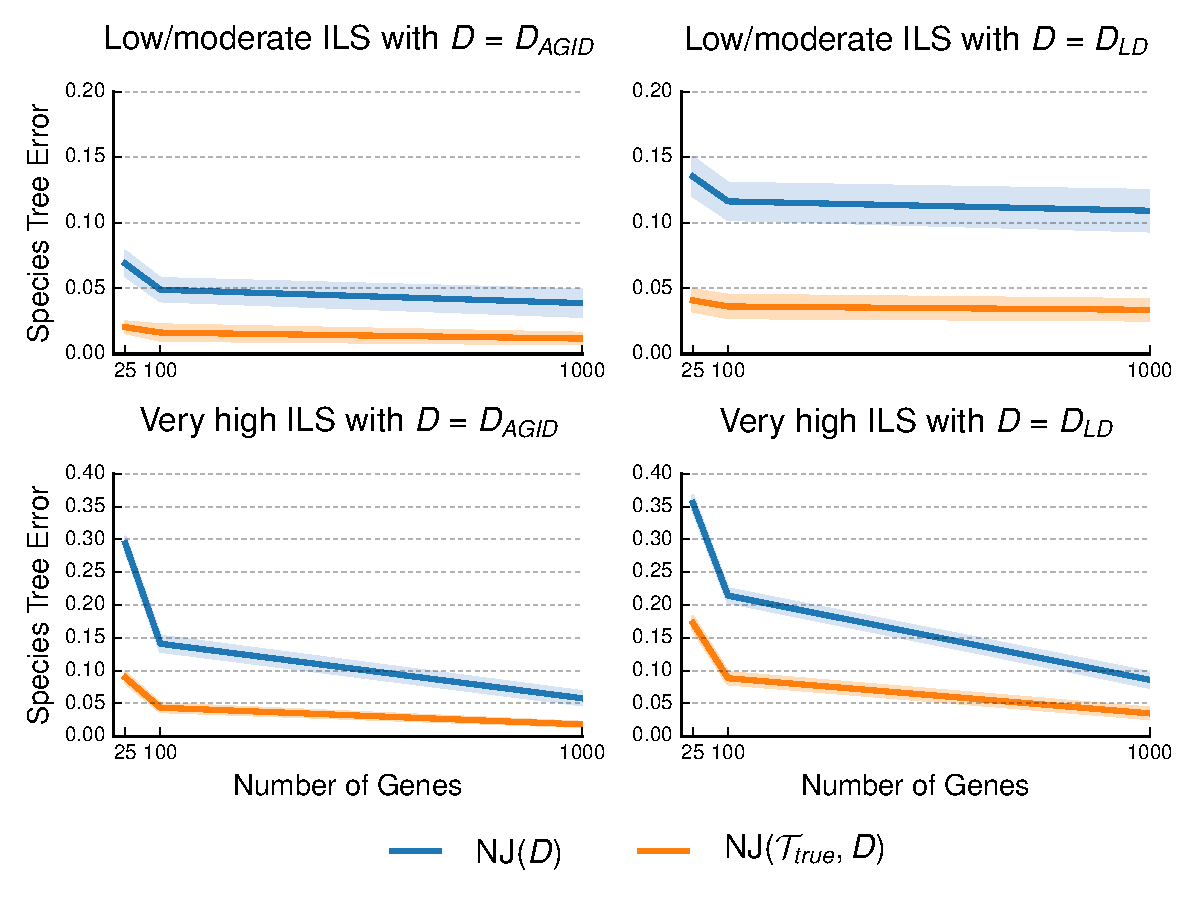
\includegraphics[width=0.95\textwidth]{figures/njmerge-fig5.pdf}
\caption{
{\bf Impact of estimated dissimilarity matrix on NJMerge. }
NJ and NJMerge were benchmarked on distance matrices estimated using two different metrics; in addition, NJMerge was given constraint trees that agreed with the true species tree (see Section~\ref{sec:njmerge-study} for notation).
Datasets had 100 species, 25 to $1\,000$ intron-like genes, and two levels of ILS.
Species tree error is the RF error rate.
Lines represent the average over replicate datasets, and filled regions indicate the standard error.
}
\label{fig:true-intron}
\end{figure}

\begin{figure}[!h]
\centering
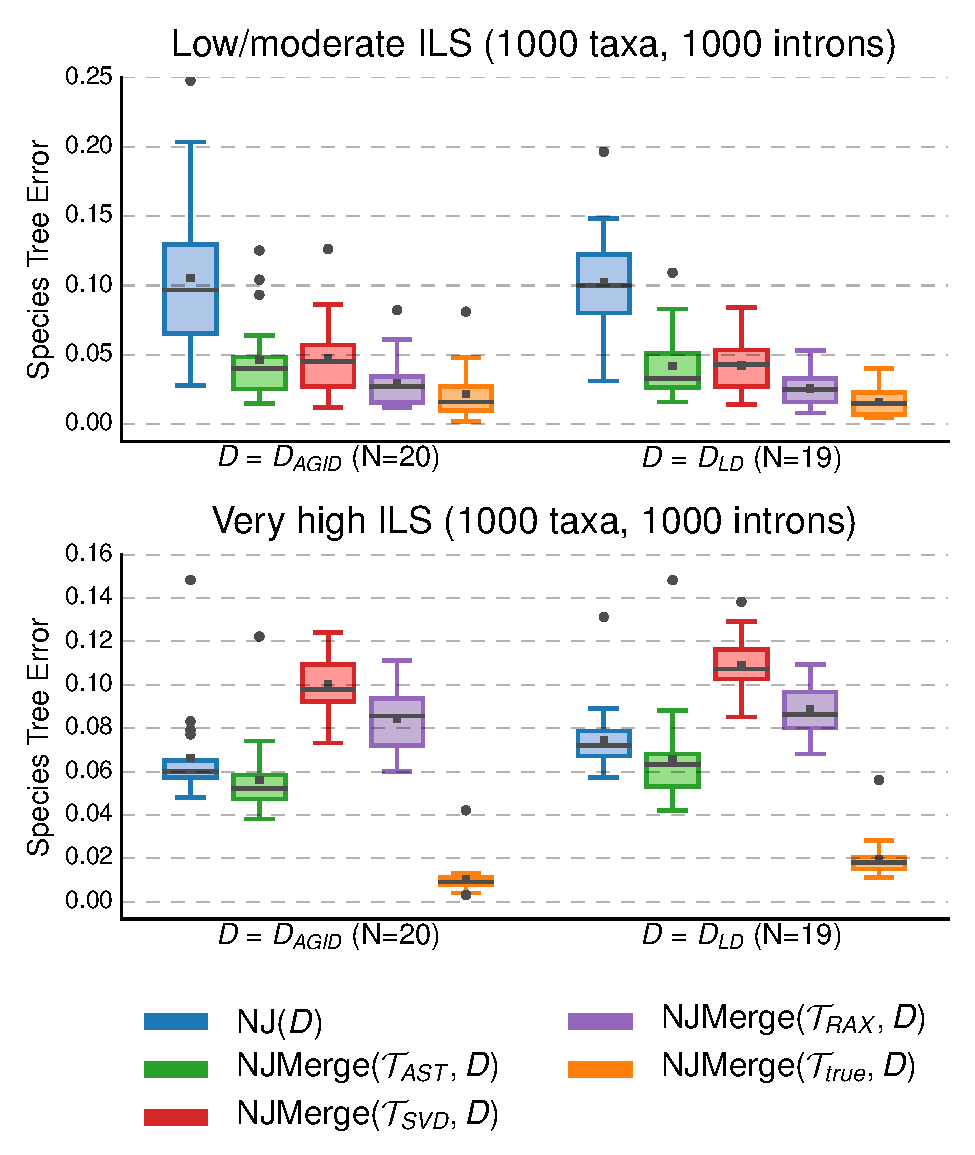
\includegraphics[width=0.72\textwidth]{figures/njmerge-fig6.pdf}
\caption{
{\bf Impact of estimated constraint trees on NJMerge. }
NJ and NJMerge were benchmarked on distance matrices estimated using two different metrics; in addition, NJMerge was given constraint trees estimated using four different techniques (see Section~\ref{sec:njmerge-study} for notation).
Datasets had $1\,000$ species, $1\,000$ intron-like genes, and two levels of ILS.
Species tree error is the RF error rate.
Gray bars represent medians, gray squares represent means, gray circles represent outliers, box plots are defined by quartiles (extending from the first to the third quartiles), and whiskers extend to plus/minus 1.5 times the interquartile distance (unless greater/less than the maximum/minimum value).
}
\label{fig:compare-1000-intron}
\end{figure}

\begin{figure}[!h]
\centering
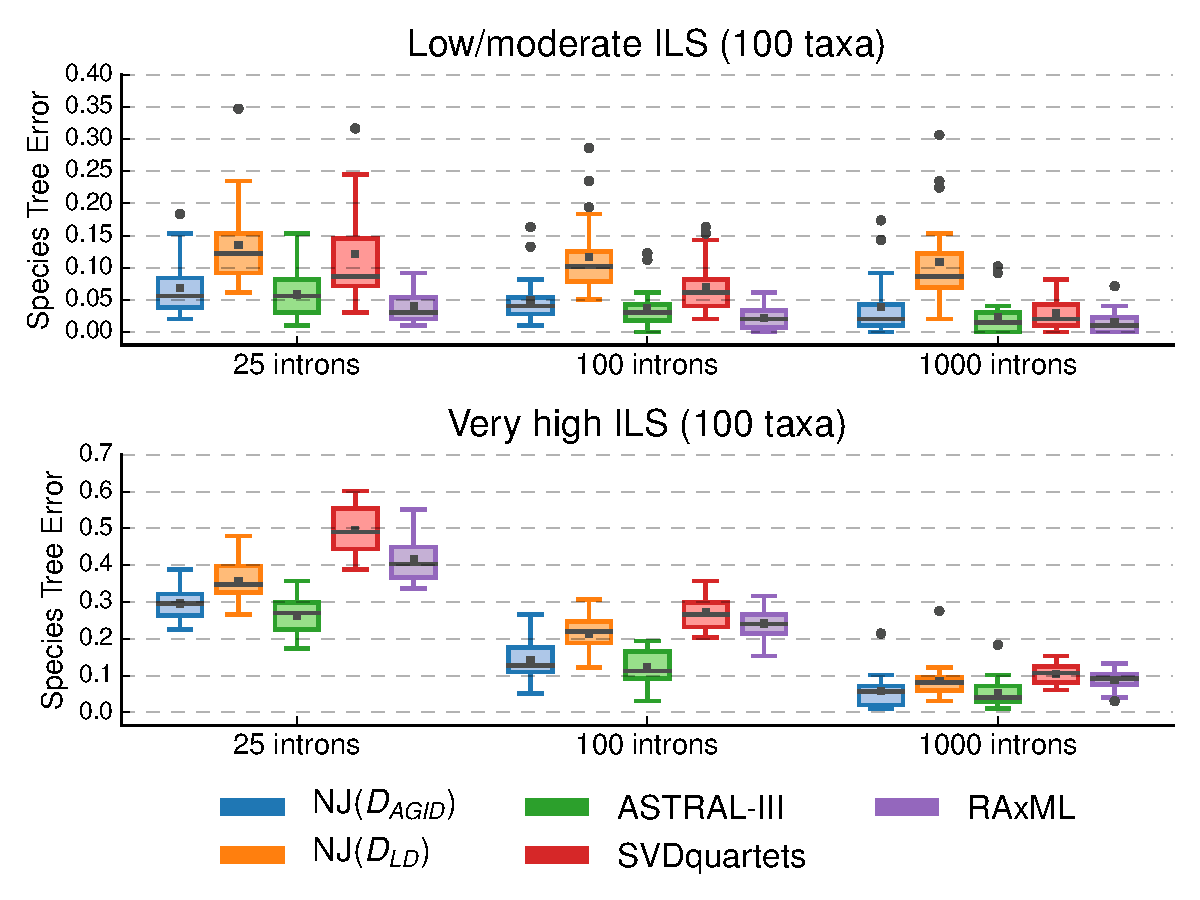
\includegraphics[width=\textwidth]{figures/njmerge-fig7.pdf}
\caption{
{\bf Comparison of species tree methods. }
NJ was benchmarked on distance matrices estimated using two different metrics (see Section~\ref{sec:njmerge-study} for notation).
Datasets had 100 species, 25 to $1\,000$ intron-like genes, and two levels of ILS.
Species tree estimation error is the RF error rate.
Gray bars represent medians, gray squares represent means, gray circles represent outliers, box plots are defined by quartiles (extending from the first to the third quartiles), and whiskers extend to plus/minus 1.5 times the interquartile distance (unless greater/less than the maximum/minimum value).
}
\label{fig:compare-100-intron}
\end{figure}

\begin{figure}[!h]
\centering
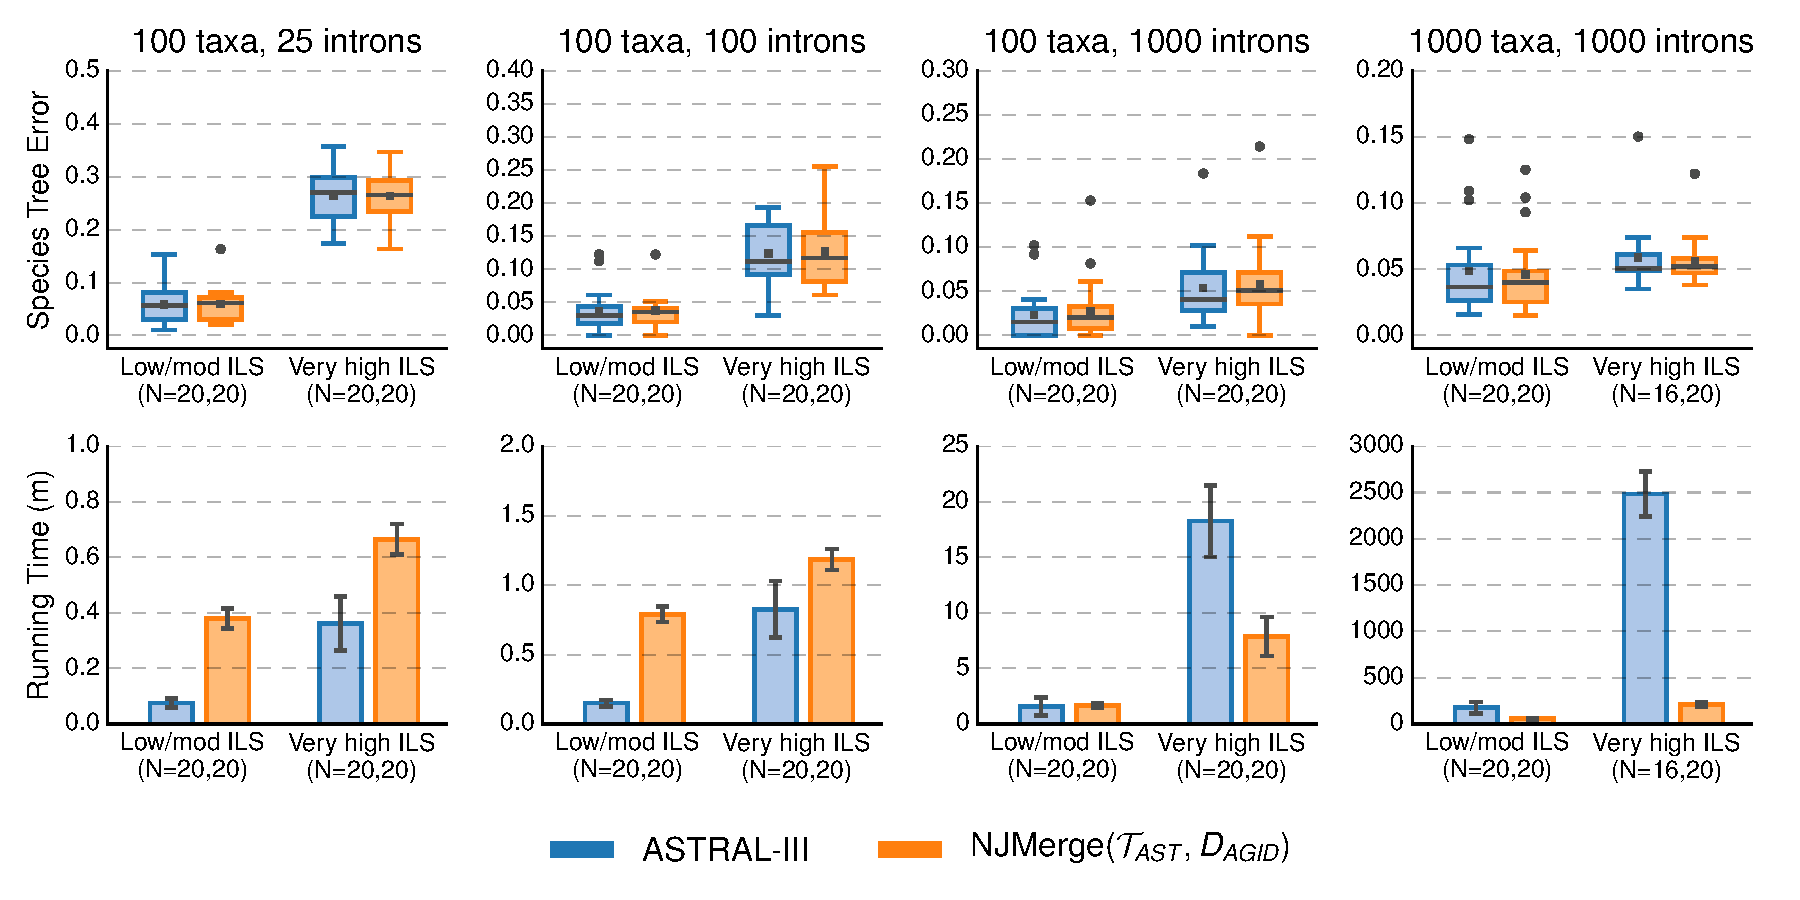
\includegraphics[width=\textwidth]{figures/njmerge-fig8.pdf}
\caption{
{\bf ASTRAL-III vs. NJMerge given ASTRAL-III constraint trees and AGID matrix. }
Subplots in the top row show species tree error (RF error rate).
Gray bars represent medians, gray squares represent means, gray circles represent outliers, box plots are defined by quartiles (extending from the first to the third quartiles), and whiskers extend to plus/minus 1.5 times the interquartile distance (unless greater/less than the maximum/minimum value).
Subplots in the bottom row show running time (in minutes); bars represent means and error bars represent standard deviations across replicate datasets.
NJMerge running times are for computing the subset trees in a  serialized fashion (Equation~\ref{eq:serial}).
The numbers of replicates on which the methods completed is shown on the $x$-axis; for example, $N=X,Y$ indicates that ASTRAL-III completed on $X$ out of 20 replicates and that NJMerge($\mathcal{T}_{AST},D_{AGID}$) completed on $Y$ out of 20 replicates.
ASTRAL-III did not complete within the maximum wall-clock time of 48 hours on 4/40 intron-like datasets with $1\,000$ species (taxa) and very high ILS.
}
\label{fig:astral-intron}
\end{figure}

\begin{figure}[!h]
\centering
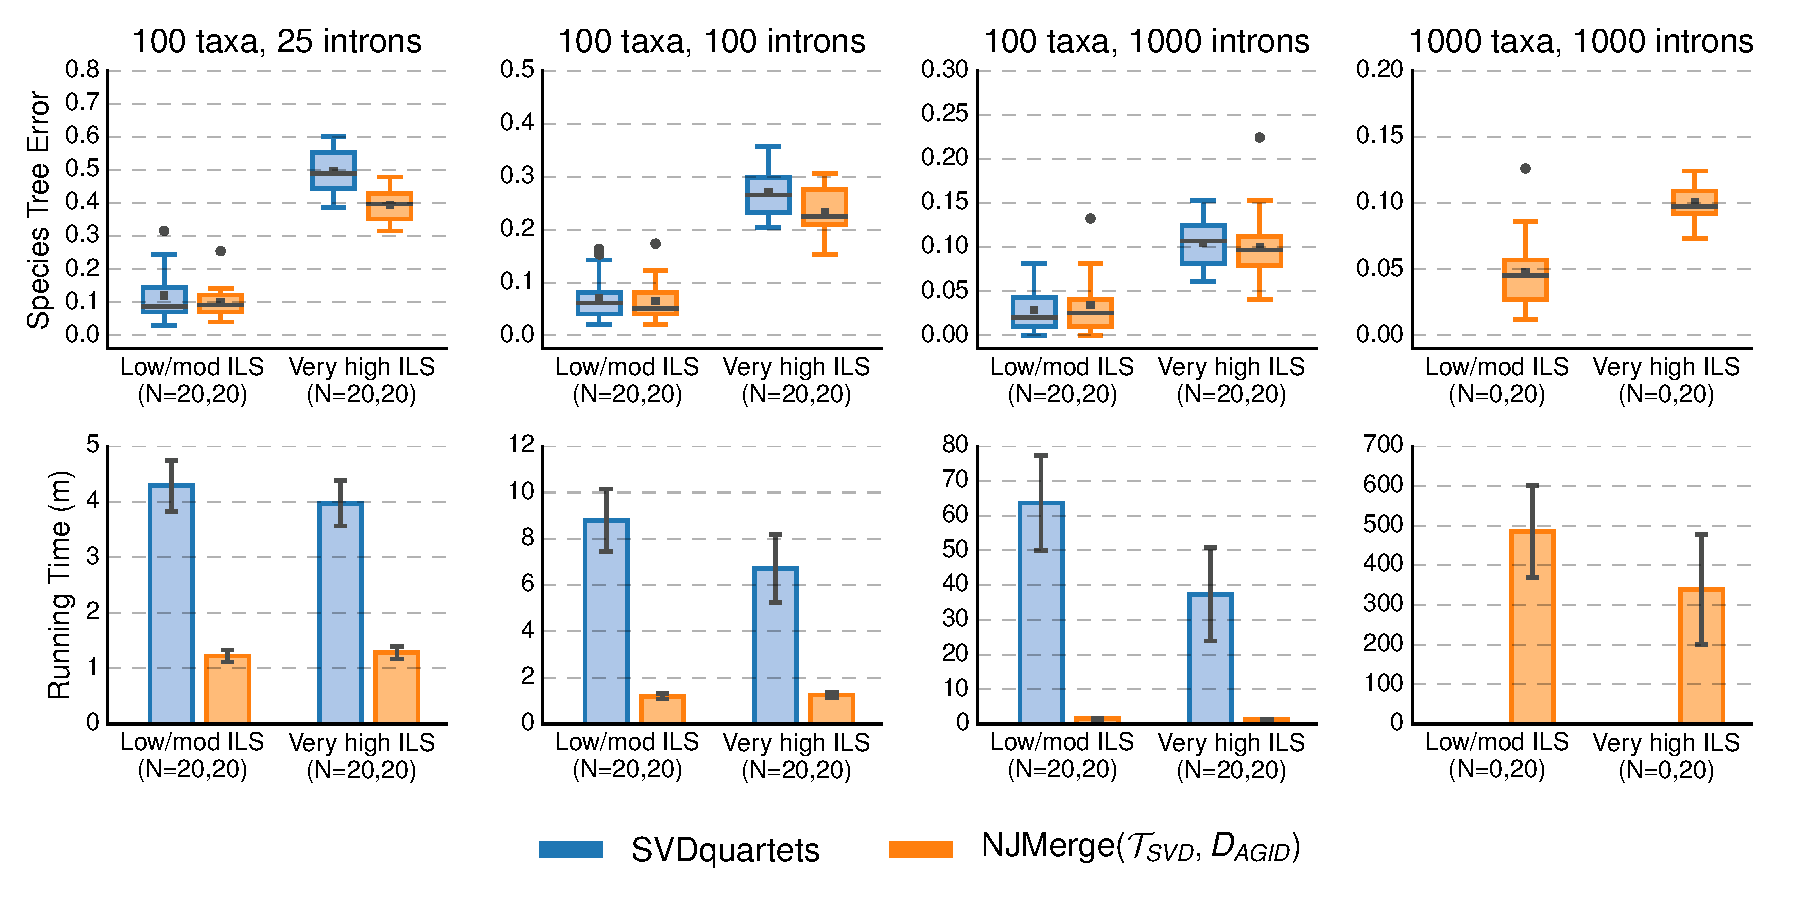
\includegraphics[width=\textwidth]{figures/njmerge-fig9.pdf}
\caption{
{\bf SVDquartets vs. NJMerge given SVDquartet constraint trees and AGID matrix. }
Subplots in the top row show species tree error (RF error rate).
Gray bars represent medians, gray squares represent means, gray circles represent outliers, box plots are defined by quartiles (extending from the first to the third quartiles), and whiskers extend to plus/minus 1.5 times the interquartile distance (unless greater/less than the maximum/minimum value).
Subplots in the bottom row show running time (in minutes); bars represent means and error bars represent standard deviations across replicate datasets.
NJMerge running times are for computing the subset trees in a  serialized fashion (Equation~\ref{eq:serial}).
The numbers of replicates on which the methods completed is shown on the $x$-axis; for example, $N=X,Y$ indicates that SVDquartets completed on $X$ out of 20 replicates and that NJMerge($\mathcal{T}_{SVD},D_{AGID}$) completed on $Y$ out of 20 replicates.
SVDquartets did not run any datasets with $1\,000$ species (taxa) due to segmentation faults.
}
\label{fig:svdq-intron}
\end{figure}

\begin{figure}[!h]
\centering
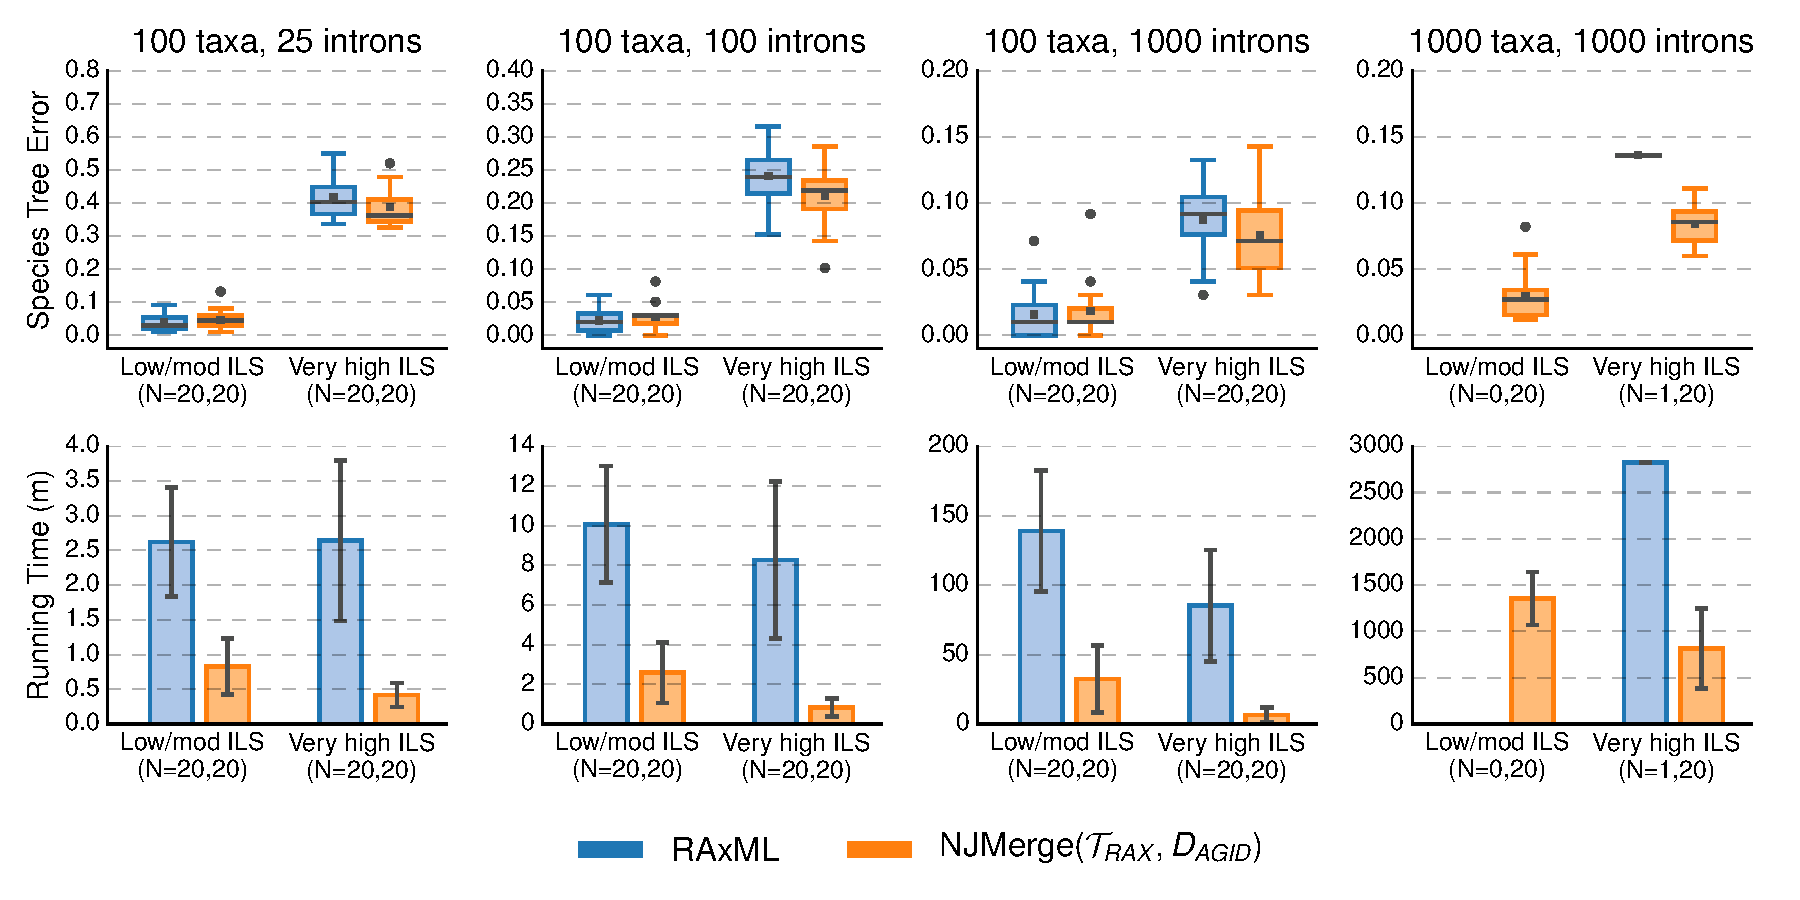
\includegraphics[width=\textwidth]{figures/njmerge-fig10.pdf}
\caption{
{\bf RAxML vs. NJMerge given RAxML constraint trees and and AGID matrix. }
Subplots in the top row show species tree error (RF error rate).
Gray bars represent medians, gray squares represent means, gray circles represent outliers, box plots are defined by quartiles (extending from the first to the third quartiles), and whiskers extend to plus/minus 1.5 times the interquartile distance (unless greater/less than the maximum/minimum value).
Subplots in the bottom row show running time (in minutes); bars represent means and error bars represent standard deviations across replicate datasets.
NJMerge running times are for computing the subset trees in a serialized fashion (Equation~\ref{eq:serial}).
The numbers of replicates on which the methods completed is shown on the $x$-axis; for example, $N=X,Y$ indicates that RAxML completed on $X$ out of 20 replicates and that NJMerge($\mathcal{T}_{RAX},D_{AGID}$) completed on $Y$ out of 20 replicates.
RAxML was only able to run on 1/40 intron-like datasets with $1\,000$ species (taxa) due to ``Out of Memory'' errors.
}
\label{fig:raxml-intron}
\end{figure}

\afterpage{\clearpage}
\newpage

\section{Table}
\label{sec:njmerge-tables}
This section contains the table presented in Section~\ref{sec:njmerge-results} Results.

\vspace{12pt}

\begin{table}[!h]
\caption{{\bf Failures. } The number of datasets on which methods failed is indicated by model condition.
ASTRAL-III failed due to running beyond the maximum wall clock time of 48 hours, SVDquartets failed due to segmentation faults, RAxML failed due to running out of memory, and NJMerge failed due to being unable to find a legal siblinghood. 
Note that NJMerge is described by the input set $\mathcal{T}$ of constraint trees  and input dissimilarity matrix $D$ (see Section~\ref{sec:njmerge-study} for notation).
}\label{tab:fail}
\centering
\begin{tabular}{cccccc}
\toprule
\# of & \# of & ILS & Sequence & Method & \# of Failures \\
Species & Genes & Level & Type & & (out of 20)  \\
\midrule
100 & 25 & very high & exon & NJMerge($\mathcal{T}_{true}$, $D_{LD}$) & 1\\
100 & 25 & very high & exon & NJMerge($\mathcal{T}_{RAX}$, $D_{AGID}$) & 1\\
100 & 25 & very high & intron & NJMerge($\mathcal{T}_{true}$,$ D_{AGID}$) & 1\\
$1\,000$ & $1\,000$ & low/moderate & exon & SVDquartets & 20\\
$1\,000$ & $1\,000$ & low/moderate & exon & RAxML & 3\\
$1\,000$ & $1\,000$ & low/moderate & intron & NJMerge($\mathcal{T}_{AST}$, $D_{LD}$) & 1\\
$1\,000$ & $1\,000$ & low/moderate & intron & SVDquartets & 20\\
$1\,000$ & $1\,000$ & low/moderate & intron & RAxML & 20\\
$1\,000$ & $1\,000$ & very high & exon & ASTRAL-III & 19\\
$1\,000$ & $1\,000$ & very high & exon & NJMerge($\mathcal{T}_{true}$, $D_{LD}$) & 1\\
$1\,000$ & $1\,000$ & very high & exon & NJMerge($\mathcal{T}_{AST}$, $D_{LD}$) & 1\\
$1\,000$ & $1\,000$ & very high & exon & NJMerge($\mathcal{T}_{SVD}$, $D_{LD}$) & 2\\
$1\,000$ & $1\,000$ & very high & exon & NJMerge($\mathcal{T}_{RAX}$, $D_{LD}$) & 2\\
$1\,000$ & $1\,000$ & very high & exon & SVDquartets & 20\\
$1\,000$ & $1\,000$ & very high & intron & ASTRAL-III & 4\\
$1\,000$ & $1\,000$ & very high & intron & NJMerge($\mathcal{T}_{SVD}, D_{LD}$) & 1\\
$1\,000$ & $1\,000$ & very high & intron & SVDquartets & 20\\
$1\,000$ & $1\,000$ & very high & intron & RAxML & 19\\
\bottomrule
\end{tabular}
\end{table}

\afterpage{\clearpage}
\newpage

\section{Algorithms}
\label{sec:njmerge-algorithms}
This section contains the three algorithms presented in Section~\ref{sec:njmerge-approach} Approach.

\vspace{12pt}

\begin{algorithm}[!h]
\footnotesize
\setstretch{1.15}
\caption{{\bf NJMerge.}}
\label{alg:njmerge}
\DontPrintSemicolon
\SetAlgoNoLine
\SetAlgoNoEnd
\SetKwInOut{Input}{Input}
\SetKwInOut{Output}{Output} 
\SetKwFunction{NJMerge}{NJMerge}
\SetKwFunction{RunCompatiblityHeuristicAndUpdateConstraints}{RunCompatiblityHeuristicAndUpdateConstraints}
\SetKwFunction{UpdateTree}{UpdateTree}
\SetKwFunction{UnrootTree}{UnrootTree}
\SetKwFunction{String}{String}
\SetKwProg{Pn}{Function}{:}{}
\vspace{.1in}
\Input{Set $\mathcal{T} = \{T_i \}_{i=1}^k$ of unrooted phylogenetic trees such that $S(T_i) \cap S(T_j) = \emptyset$ $\forall \; i \ne j$ and an $n \times n$ dissimilarity matrix $D$ on label set $S = \bigcup_{i=1}^k S(T_i)$}
\Output{A (possibly refined) compatibility supertree for $\mathcal{T}$ that is fully resolved}
\vspace{-4pt}

\hrulefill

\Pn{\NJMerge{$\mathcal{T}$, $D$}}{
	$I \leftarrow \{1, 2, \dots, n\}$; $S \leftarrow$ list version of $S$\;
	Relabel $T_i \in \mathcal{T}$, so a leaf labeled $s$ is now labeled $i$ if row $i$ in $D$ is labeled $s$\;
	\lFor{$i \in I$}{$r[i] \leftarrow \sum_{j \in I} D[i,j]$}
	\vspace{10pt}
	\While{$| I | > 3$}{
		\vspace{10pt}
		{\bf Step 1:} Build $Q$, so that $Q[i, j] \leftarrow (| I | -2) D[i,j] - r[i] - r[j]$ $\forall \; i,j \in I$,  and simultaneously sort $Q$ from smallest to largest, producing the vector $sorted$.\; 
		\vspace{10pt}
		{\bf Step 2:} Select next sibling pair $(x,y)$ to join.\;
		\For{$i \in \{1, 2, \dots, (|I|^2 - |I|)/2\}$}{
			$(x,y) \leftarrow sorted[i]$\;
			$pass \leftarrow $ \RunCompatiblityHeuristicAndUpdateConstraints{$\mathcal{T}$, $x$, $y$}\;
			\lIf{$pass$}{break}
		}
		\lIf{not $pass$}{\Return{} $fail$}
		\vspace{10pt}
		{\bf Step 3a:} Update $D$.\;
		$\vec{dx} \leftarrow [0]_n$; $dxy \leftarrow D[x,y]$\;
		\For{$i \in I \setminus \{ x, y \}$}{
			$dx[i] \leftarrow D[x,i]$\;
			$D[x, i] \leftarrow \frac{1}{2} \big( dx[i] + D[y, i] - dxy \big)$; $D[i,x] \leftarrow D[x,i]$\;
		}
		\vspace{10pt}
		{\bf Step 3b:} Update $\vec{r}$.\;
		\For{$i \in I \setminus \{ x, y \}$}{
			$r[i] \leftarrow r[i] - dx[i] - D[y,i] + D[x, i]$\;
		}
		$r[x] \leftarrow \sum_{i \in I \setminus\{ x, y \}} D[x, i]$\;
		\vspace{10pt}
		{\bf Step 3c:} Update indices and labels.\;
		 $I \leftarrow I \setminus \{ y \}$\;
		 $S[x] \leftarrow$ `(' + S[x] + `,'+ S[y] + `)'\;
	}
	\vspace{10pt}
	$T \leftarrow [NULL]_3$;
	$j \leftarrow1 $\;
	\For{$i \in I$}{
		$T[j] \leftarrow L[i]$;
		$j \leftarrow j + 1$\;
	}
	\vspace{10pt}
	\Return{\emph{`(' + T[1] + `,'+ T[2] + `,' + T[3] + `);'}}\;
}
\vspace{3pt}
\end{algorithm}

\clearpage

\begin{algorithm}[!h]
\footnotesize
\setstretch{1.15}
\caption{{\bf RunCompatiblityHeuristicAndUpdateConstraints.} We assume that the representation of each constraint tree $T$ uses $O(n)$ space and includes an $n$-vector $L(T)$ of leaf nodes, so that the element at position $i$ is either the leaf with label $i$ or $NULL$ if there is no leaf with label $i$. This allows leaf nodes to be accessed by their labels in constant time.}
\label{alg:heuristic-compatibility}
\DontPrintSemicolon
\SetAlgoNoLine
\SetAlgoNoEnd
\SetKwInOut{Input}{Input}
\SetKwInOut{Output}{Output} 
\SetKwFunction{IsCompatibleHeuristic}{IsCompatibleHeuristic}
\SetKwFunction{RunCompatiblityHeuristicAndUpdateConstraints}{RunCompatiblityHeuristicAndUpdateConstraints}
\SetKwFunction{PruneLeaf}{PruneLeaf}
\SetKwFunction{UpdateTree}{UpdateTree}
\SetKwFunction{RelabelLeaf}{RelabelLeaf}
\SetKwFunction{AddSibling}{AddSibling}
\SetKwFunction{IsSiblingPair}{IsSiblingPair}
\SetKwFunction{ReverseUpdateTree}{ReverseUpdateTree}
\SetKwProg{Pn}{Function}{:}{}
\vspace{.1in}
\Input{Set $\mathcal{T} = \{T_1, T_2, \dots, T_k \}$ of unrooted phylogenetic trees and labels $x, y \in S = \bigcup_{i=1}^k S(T_i)$}
\Output{$true$ if the test passes, and $false$ otherwise}
\vspace{-4pt}

\hrulefill

\Pn{\RunCompatiblityHeuristicAndUpdateConstraints{$\mathcal{T}$, $x$, $y$}}{
	\For{$i \in \{1, 2, \dots, k \}$}{
		$L \leftarrow L(T_i)$\;
		\If{$L[x] \ne NULL$ and $L[y] \ne NULL$}{
			\lIf{not \IsSiblingPair{$T_i$, $x$, $y$}}{\Return{$fail$}}
		}
	}

	$\mathcal{P} = \emptyset$;
	$update \leftarrow [0]_k$\;
	\For{$i \in \{1, 2, \dots, k \}$}{
		$update[i] \leftarrow $ \UpdateTree{$T_i$, $x$, $y$}\;
		\If{$update[i] \ne 0$}{
			$\mathcal{P} \leftarrow \mathcal{P} \cup T_i$\;
		}
	}
	\lIf{\IsCompatibleHeuristic{$\mathcal{P}$}}{\Return{$true$}}
	\lFor{$i \in \{1, 2, \dots, k \}$}{
		\ReverseUpdateTree{$T_i$, $x$, $y$, $update[i]$}
	}
	\Return{$fail$}
}
\vspace{10pt}
\Pn{\UpdateTree{$T$, $x$, $y$}}{
	$L \leftarrow L(T)$\;
	\If{$L[x] \ne NULL$ and $L[y] \ne NULL$}{
		$update \leftarrow 1$; \PruneLeaf{$T$, $y$}\;
	}
	\ElseIf{$L[y] \ne NULL$}{
		$update \leftarrow 2$; \RelabelLeaf{$T$, $y$, $x$};
	}\ElseIf{$L[x] \ne NULL$}{
		$update \leftarrow 3$\;
	}
	\Return{update}\;
}
\vspace{10pt}
\Pn{\ReverseUpdateTree{$T$, $x$, $y$, $update$}}{
	\If{$update = 1$}{
		\AddSibling{$T$, $x$, $y$}\;
	}\ElseIf{$update = 2$}{
		\RelabelLeaf{$T$, $x$, $y$}\;
	}
}
\vspace{3pt}
\end{algorithm}

\clearpage

\begin{algorithm}[!h]
\footnotesize
\setstretch{1.15}
\caption{{\bf IsCompatibleHeuristic.} We assume that the representation of each constraint tree $T$ uses $O(n)$ space and includes an $n$-vector $L(T)$ of leaf nodes, so that the element at position $i$ is either the leaf with label $i$ or $NULL$ if there is no leaf with label $i$. This allows leaf nodes to be accessed by their labels in constant time. Note that this is a naive implementation.}
\label{alg:pairwise}
\DontPrintSemicolon
\SetAlgoNoLine
\SetAlgoNoEnd
\SetKwInOut{Input}{Input}
\SetKwInOut{Output}{Output} 
\SetKwFunction{ComputeRF}{ComputeRF}
\SetKwFunction{PruneLeaf}{PruneLeaf}
\SetKwFunction{CopyTree}{CopyTree}
\SetKwFunction{DeleteTree}{DeleteTree}
\SetKwFunction{RestrictTree}{RestrictTree}
\SetKwProg{Pn}{Function}{:}{}
\vspace{.1in}
\Input{Set $\mathcal{P} = \{ T_1, T_2, \dots, T_p \}$ of unrooted phylogenetic trees}
\Output{$true$ if the test passes, and $false$ otherwise}
\vspace{-4pt}

\hrulefill

\Pn{\IsCompatibleHeuristic{$\mathcal{P}$}}{
	\For{$i \in \{1, 2, \dots, p-1 \}$}{
		\For{$j \in \{i+1, \dots, p \}$}{
			$L_i \leftarrow L(T_i)$;
			$L_j \leftarrow L(T_j)$\;
			$R \leftarrow \emptyset$\;
			\For{$s \in S(T_i) \cap S(T_j)$}{
				\If{$L_i[s] \ne NULL$ and $L_j[s] \ne NULL$}{
					$R \leftarrow R \cup \{ s \}$\;
				}
			}
			$P_{i}' \leftarrow $ \CopyTree{$P_i$}; 
			\RestrictTree{$P_{i}'$, $R$}\;
			 $P_{j}' \leftarrow $ \CopyTree{$P_j$};
			\RestrictTree{$P_{j}'$, $R$}\;
			$rf \leftarrow$ \ComputeRF{$P_i'$, $P_j'$}\;
			\DeleteTree{$P_i'$};
			\DeleteTree{$P_j'$}\;
			\If{$rf > 0$}{
				\Return{$false$}\;
			}
		}
	}
	\Return{$true$}
}
\vspace{10pt}
\Pn{\RestrictTree{$T$, $R$}}{
	\For{$l \in S(T) \setminus R$}{
		\PruneLeaf{$T$, $l$}\;
	}
}
\vspace{3pt}
\end{algorithm}

\chapter{Divide-and-Conquer Pipelines with TreeMerge}
\label{chapter:treemerge}
\textit{This chapter contains material previously published in ``TreeMerge: a new method for improving the scalability of species tree estimation methods'' \cite{molloy2019treemerge}, which was joint work with T. Warnow.
Software commands necessary to reproduce this study are freely available on the Illinois Data Bank:~\href{https://doi.org/10.13012/B2IDB-9570561_V1}{doi.org/10.13012/B2IDB-9570561\_V1}.
\emph{TreeMerge} is freely available on Github:~\href{https://github.com/ekmolloy/treemerge}{github.com/ekmolloy/treemerge}.
Note that plots and tables appear at the end of this chapter in Sections~\ref{sec:treemerge-plots} and \ref{sec:treemerge-tables}, respectively.}
\glsreset{DTM}
\glsreset{RF}
\glsreset{MSC}
\glsreset{GTR}
\glsreset{MSA}
\glsreset{ML}
\glsreset{ILS}
\section{Introduction}
In Chapter~\ref{chapter:njmerge}, we proposed an alternative approach to divide-and-conquer that operates by
\begin{enumerate*}[label=(\roman*)]
	\item 
	dividing the species set into pairwise disjoint subsets of a predetermined maximum size, 
	\item 
	estimating a tree on each subset, 
	\item
	computing any auxiliary data required for \glspl{merge} subset trees, and then
	\item
	 using the auxiliary data to merge the subset trees together into a \gls{compatibilitysupertree} (Definition~\ref{def:compatibility-supertree}).
\end{enumerate*}
For the final step, we presented \gls{NJMerge}, a \gls{DTM} method that uses a \gls{dissimilaritymatrix} to build a (possibly refined) compatibility supertree for the subset trees.
Despite its promising theoretical and empirical results, NJMerge has two major issues that limit its utility in practice.
First, NJMerge can fail to return a tree, and second, the worst-case running time of NJMerge is $O(n^4k)$, where the input has $n$ species (leaf labels) divided across $k$ \gls{leaf-label-disjoint} trees.

In this chapter, we address the limitations of NJMerge by presenting new methods, all of which are guaranteed to return a compatibility supertree when given (\gls{fullyresolved}) leaf-label-disjoint trees as input.
The first method, NJMerge-2, is a minor modification to NJMerge; it has the same theoretical properties as NJMerge except that it does not fail.
The second method, \textit{\gls{TreeMerge}}, seeks to address the scalability issue by merging subset trees in two phases: a \textit{\gls{localmergephase}} and a \textit{\gls{globalmergephase}}.
In the local merge phase, a highly accurate but computationally intensive method is used to merge leaf-label-disjoint trees in an embarrassingly parallel fashion. 
In the global merge phase, the trees computed during the local merge phase are then combined via a reduction.
Within the divide-and-conquer framework, TreeMerge runs in $O(n \log{n})$ time or in $O(n^2)$ time if the reduction is serialized. 
This running time analysis assumes that the mergers during the global phase are performed using a linear-time technique.

As we will show, the linear-time merge operation constrains the space of allowed solutions, which in turn places some additional (but achievable) requirements for divide-and-conquer pipelines using TreeMerge to be \gls{statisticallyconsistent} (as compared to those using NJMerge or NJMerge-2).
Nevertheless, the results of our simulation study show that \glspl{speciestree} estimated using TreeMerge can be quite accurate, comparing favorably to those estimated by other DTM-based divide-and-conquer pipelines or traditional species tree estimation methods (\gls{ASTRAL}-III and \gls{CA-ML} using \gls{RAxML}).
Like NJMerge, TreeMerge enables the dominant species tree estimation methods to scale to larger datasets without sacrificing accuracy.
Unlike NJMerge, TreeMerge is guaranteed to return a compatibility supertree, is much faster (in terms of its worst-case running time), and is more easily parallelizable, making it a notable advance for large-scale \gls{phylogeny} estimation.

\section{Approach}
\label{sec:approach}
We now present the NJMerge-2 and TreeMerge algorithms focusing on worst-case running time, correctness, and statistical consistency within divide-and-conquer pipelines.

\subsection{NJMerge-2} 
NJMerge-2 is a simple extension to NJMerge so that it is guaranteed to return a compatibility supertree for the input constraint (subset) trees.
Recall that NJMerge modifies \gls{NJ} by imposing a set of topological constraints on the output tree.
For each siblinghood proposal, NJMerge updates the constraint trees based on the proposed siblinghood and then tests the compatibility of the updated constraint trees; if the test passes, NJMerge accepts the siblinghood proposal.
Because determining the compatibility of a set of  $k$ unrooted trees on overlapping leaf label sets is NP-complete \cite{steel1992complexity}, NJMerge uses a heuristic that can fail for $k > 2$ trees.
Therefore, by running NJMerge on two constraint trees at a time, it will never fail; this observation is the basis of NJMerge-2 (Algorithm~\ref{alg:njmerge2}). 

\begin{theorem}
\label{thm:njmerge2-rt-correct}
Let $\mathcal{T} = \{T_1, T_2, \dots, T_k\}$ be a set of \gls{unrooted} \glspl{phylogenetictree} such that $S(T_i) \cap S(T_j) = \emptyset$ for all $i \ne j$, and let $D$ be an $n \times n$ \gls{dissimilaritymatrix}  on label set $S = \cup_{i=1}^k S(T_i)$.
Then, NJMerge-2 applied to input $(\mathcal{T}, D)$ returns a (possibly refined) compatibility supertree for $\mathcal{T}$ in $O(n^4k)$ time; the parallel version of NJMerge-2 runs in $O(n^4)$ time.
Furthermore, if $D$ is a \gls{nearlyadditive} matrix for a fully resolved tree $T^*$ on label set $S$ (Definition~\ref{def:nearly-additive}) and if $T^*$ is \gls{compatible} with $T_i$ for all $i \in \{1, \dots, k\}$ (Definition~\ref{def:compatibility}), then NJMerge-2 returns $T^*$.
\end{theorem}

\begin{proof}
\emph{Returns a compatibility supertree:} It is easy to see that the constraint trees remain leaf-label-disjoint and thus compatible at each iteration, and because the heuristics used by NJMerge correctly determine compatibility for two trees, NJMerge applied to the input $\big( \{ t, t' \}, D|_{S(t) \cup S(t')} \big)$ is guaranteed to return a (possibly refined) compatibility supertree (Theorem~\ref{thm:njmerge}).
By induction on the number of constraint trees, NJMerge-2 returns a (possibly refined) compatibility supertree for $\mathcal{T}$.

\emph{Correctness:} If, in addition, the trees in $\mathcal{T}$ are compatible with $T^*$ and the dissimilarity matrix $D$ is nearly additive for $T^*$, then for any pair of trees $t, t' \in \mathcal{T}$, NJMerge applied to the input $\big( \{ t, t' \}, D|_{S(t) \cup S(t')} \big)$ returns $T^*|_{S(t) \cup S(t')}$ (Theorem~\ref{thm:njmerge-correct}).
Therefore, the set $\mathcal{T}$ remains compatible with $T^*$ during the iterative process.
By induction on the number of constraint trees, NJMerge-2 returns $T^*$.

\emph{Running time:} For the running time analysis, we make the simplifying assumption that each of the $k$ trees in $\mathcal{T}$ has exactly $n/k$ leaves.
At iteration $w$, for any two trees $t, t' \in \mathcal{T}$, $ |S(t) \cup S(t') | \le (w + 1)n/k$, so the worst-case running time of NJMerge given any pair of trees is $O(w^4 n^4 / k^4)$ (Theorem~\ref{thm:njmerge}).
A total of $k-1$ iterations are required, so the running time of NJMerge-2 scales with $(n^4/k^4) \sum_{w=2}^k w^4$. 
Because $\sum_{w=2}^k w^4$ is $O(k^5)$, the worst-case running time of NJMerge-2 is $O(n^4k)$. Although Algorithm~\ref{alg:njmerge2} runs NJMerge-2 on pairs of trees in serial, we could consider a parallel version of NJMerge-2. 
Assuming that $k$ is a power of two for simplicity, at iteration $w$, we run NJMerge on each of the $k/(2^w)$ pairs of trees in parallel, where for any pair of trees  $t, t' \in \mathcal{T}$, $ |S(t) \cup S(t') | = 2^{w}n/k$.
A total of $p = \log_2{(k)} - 1$ iterations are required, so the parallel running time of NJMerge scales with $(n^4/k^4) \sum_{w=2}^p 2^{4w}$ and thus is $O(n^4)$.
This is expected as the running time of NJMerge-2 is dominated by the time to run NJMerge in the final iteration.
\end{proof}

\vspace{12pt}

\begin{algorithm}[!h]
\footnotesize
\setstretch{1.15}
\caption{{\bf NJMerge-2.}}
\label{alg:njmerge2}
\DontPrintSemicolon
\SetAlgoNoLine
\SetAlgoNoEnd
\SetKwInOut{Input}{Input}
\SetKwInOut{Output}{Output} 
\SetKwFunction{NJMerge}{NJMerge}
\SetKwFunction{NJMergeTwoSerial}{NJMergeTwoSerial}
\SetKwFunction{SelectPair}{SelectPair}
\SetKwFunction{CopyMatrixRestricted}{CopyMatrixRestricted}
\SetKwFunction{DeleteMatrix}{DeleteMatrix}
\SetKwProg{Pn}{Function}{:}{}
\vspace{.1in}
 \Input{Set $\mathcal{T} = \{T_i \}_{i=1}^k$ of  unrooted phylogenetic tree such that $S(T_i) \cap S(T_j) = \emptyset$ for all $i \ne j$ and an $n \times n$ dissimilarity matrix $D$ on label set $S_{i=1}^k \bigcup S_i$}
\Output{A (possibly refined) compatibility supertree for $\mathcal{T}$ that is fully resolved}
\vspace{-4pt}

\hrulefill

\Pn{\NJMergeTwoSerial{$\mathcal{T}$, $D$, $S$}}{
	\While{$|\mathcal{T}| > 1$}{
		\vspace{10pt}
		$t, t' \leftarrow$ An arbitrary pair of trees in $\mathcal{T}$\;
		$R \leftarrow [S(t) \cup S(t')]$\;
		$D|_R \leftarrow$ \CopyMatrixRestricted{$D$, $R$} \;
		%\vspace{10pt}
		$T \leftarrow$ \NJMerge{$\{ t, t' \}$, $D|_R$, $R$}\;
		%\vspace{10pt}
		\DeleteMatrix{$D|_R$}\;
		%\vspace{10pt}
		$\mathcal{T} \leftarrow \big( \mathcal{T} \setminus \{ t, t' \} \big) \cup \{ T \}$\;
		\vspace{10pt}
	}
	\Return{$T$}\;
 }
 \vspace{3pt}
\end{algorithm}

We do not specify an order for merging pairs of constraint trees in Algorithm~\ref{alg:njmerge2}.
While the order does not impact the theoretical guarantees of NJMerge-2, it likely impacts performance (accuracy) in practice. 
Consider a collection of constraint trees that are \gls{edgeseparable} for a \gls{caterpillartree} $T$ with a very large \textit{\gls{evolutionarydiameter}} (the longest evolutionary distance between any pair of leaves in a phylogenetic tree).
If, in the first iteration, we merge two constraint trees on opposite sides of the caterpillar tree, the output tree may contain incorrect \glspl{bipartition} due to \gls{longbranchattraction}; these incorrect bipartitions will be propagated through subsequent iterations.
Hence, it may be beneficial to perform mergers in an order that respects locality by selecting pairs of trees $t, t' \in \mathcal{T}$ based on the evolutionary distance between set $S(t)$ and set $S(t')$ in $D$. 
Exploiting locality can also be useful for improving computationally efficiency, as we will show.

\subsection{TreeMerge}
\label{sec:treemerge}
\glsreset{TreeMerge}
We now introduce TreeMerge, the first DTM method that combines an embarrassingly parallel local merge phase with a global merge phase.
As shown in Algorithm~\ref{alg:treemerge}, these two phases are enabled through the use of a \textit{\gls{mergeguidetree}} given as part of the input.
The generic TreeMerge algorithm also requires auxiliary data in order to build compatibility supertrees during both the local and the global merge phases.
The exact details of the algorithm can be implemented in a variety of ways; we present two examples: TreeMerge-fast (which was previously mentioned) and TreeMerge-slow.

\begin{itemize}
	\item \textbf{\gls{TreeMergeinput}}: 
	\begin{itemize}
		\item Set $\mathcal{T} = \{T_1, T_2, \dots, T_k\}$ of \gls{unrooted}, \gls{fullyresolved} \glspl{phylogenetictree} such that $S(T_i) \cap S(T_j) = \emptyset$ for all $i \ne j$
		\item Set $\mathcal{A}$ of auxiliary data, including
		\begin{itemize}
			\item \Gls{mergeguidetree} $\mathcal{G}$ with nodes bijectively labeled by elements of the set $\{1, 2, \dots, k\}$ such  that node $i$ corresponds to tree $T_i \in \mathcal{T}$
			\item Data that can be used to merge trees, for example
			\begin{itemize}
				\item {\em TreeMerge-fast:} Set $\mathcal{D} = \{ D^{i,j} : (i,j) \in E(\mathcal{G}) \}$ of \glspl{dissimilaritymatrix}
				\item {\em TreeMerge-slow:} Dissimilarity matrix $D$ on label set $S = \bigcup_{i=1}^k S(T_i)$
			\end{itemize}
		\end{itemize}
	\end{itemize}
	\item \textbf{\gls{TreeMergeoutput}}: \Gls{compatibilitysupertree} for $\mathcal{T}$ %that is fully resolved
\end{itemize}

\begin{algorithm}[!h]
\footnotesize
\setstretch{1.15}
\caption{{\bf Generic TreeMerge Algorithm.}}
\label{alg:treemerge}
\DontPrintSemicolon
\SetAlgoNoLine
\SetAlgoNoEnd
\SetKwInOut{Input}{Input}
\SetKwInOut{Output}{Output} 
\SetKwFunction{NJMerge}{NJMerge}
\SetKwFunction{GenericTreeMerge}{GenericTreeMerge}
\SetKwFunction{PreOrderEdgeTraversal}{PreOrderEdgeTraversal}
\SetKwFunction{UpdateTree}{UpdateTree}
\SetKwFunction{RootTreeAtEdge}{RootTreeAtEdge}
\SetKwProg{Pn}{Function}{:}{}
\vspace{.1in}
 \Input{
Set $\mathcal{T} = \{T_1, T_2, \dots, T_k\}$ of unrooted, fully resolved phylogenetic trees with constraint tree $T_i$ on label set $S_i$ such that $S_i \cap S_j = \emptyset$ for all $i \ne j$, a set $\mathcal{A}$ of auxiliary data, which includes a tree $\mathcal{G}$, called the merge guide tree, with nodes bijectively labeled by elements of the set $\{1, 2, \dots, k \}$ so that node $i$ corresponds to tree $T_i \in \mathcal{T}$.
 }
\Output{Compatibilitysupertree for $\mathcal{T}$}
\vspace{-4pt}

\hrulefill

\Pn{\GenericTreeMerge{$\mathcal{T}$, $\mathcal{A}$}}{
	\vspace{10pt}
	{\bf Local merge phase:} For each edge $(i, j) \in E(\mathcal{G})$, build a compatibility supertree $T_{i,j}$ for $\{T_i, T_j\}$ using some auxiliary data in $\mathcal{A}$\;
	\vspace{10pt}
	{\bf Global merge phase:} \;
	$(x,y) \leftarrow $ An arbitrary edge in $E(\mathcal{G})$\;
	$T \leftarrow T_{x,y}$\;
	$\mathcal{G} \leftarrow$ $\mathcal{G}$ rooted at edge $(x,y)$\;
	\For{$(i, j) \in$ \PreOrderEdgeTraversal{$\mathcal{G}$}}{
		%\vspace{10pt}
		$T \leftarrow$ Compatibility supertree for $\{T, T_{i,j}\}$ built using their \gls{backbonetree} $T|_{S(T) \cap S(T_{i,j})}$ and possibly some auxiliary data in $\mathcal{A}$\;
	}
	\vspace{10pt}
	\Return{$T$}\;
 }
\vspace{3pt}
\end{algorithm}

\vspace{6pt}

We now describe the local and global phases for TreeMerge-slow and TreeMerge-fast.

\paragraph{Local merge phase:} 
During the local merge phase, mergers are performed on pairs of trees that are local, meaning that they are connected by edges in the merge guide tree $\mathcal{G}$.
For every edge $(i, j) \in E(\mathcal{G})$, both TreeMerge-slow and TreeMerge-fast build a compatibility supertree $T_{i,j}$  by running NJMerge on the input $(\{T_i,T_j\}, D^{i,j})$.
Afterward, TreeMerge-fast uses $D^{i,j}$ to fit branch lengths to $T_{i,j}$ via the least squares approach proposed by Bryant and Waddell \cite{bryant1998rapid}.
Note that TreeMerge-fast takes $D^{i,j}$ as input, whereas TreeMerge-slow creates $D^{i,j}$ by restricting $D$ to label set $S(T_i) \cup S(T_j)$.

\paragraph{Global merge phase:} 
During the global merge phase, mergers are performed following a pre-order edge traversal of the merge guide tree $\mathcal{G}$, combining the trees computed during the local merge phase into a single tree on label set $S$ (note that this can also be implemented as a reduction; see Figure \ref{fig:reduction} for an example).
The merge technique is related to the Strict Consensus Merger \cite{warnow2001absolute, swenson2012superfine}.

We describe this merge technique in the context of merging two trees $T_{i,j}$ and $T_{j,k}$ that are compatibility supertrees for $\{T_i, T_j\} \subset \mathcal{T}$ and $\{T_j, T_k\} \subset \mathcal{T}$, respectively.
The input trees in $\mathcal{T}$ are fully resolved, so $T_{i,j}$ and $T_{j,k}$ 
%are fully resolved and thus 
induce a common tree \gls{topology} $T_j$ when restricted to their shared label set; we refer to $T_j$ as the \textit{\gls{backbonetree}}.
Each edge $e$ in $E(T_j)$ maps to a path $p_{i,j}(e)$ in $T_{i,j}$ and a path $p_{j,k}(e)$ in $T_{j,k}$.
When $p_{i,j}(e)$ or $p_{j,k}(e)$ have length greater than one, the internal nodes on those paths define subtrees that need to be inserted onto edge $e$ in the backbone tree $T_j$.
Let $V_{i,j}(e)$ denote the set of subtrees in $T_{i,j}$ that need to be attached to edge $e$, and similarly, let $V_{j,k}(e)$ denote the set of subtrees in $T_{j,k}$ that need to be attached to edge $e$.
It is easy to see that adding subtrees in the set $V_{i,j}(e) \cup V_{j,k}(e)$ to edge $e$ in an arbitrary order and then repeating this process for all edges in $E(T_j)$, produces a (possibly refined) compatibility supertree for $\{T_{i,j}, T_{j,k} \}$ and thus for $\{ T_i, T_j, T_k \}$.
If $T_{i,j}$ and $T_{j,k}$ never contribute subtrees to the same edge, $T_{i,j,k}$ is the unique compatibility supertree for $\{ T_i, T_j, T_k \}$; otherwise, $T_{i,j,k}$ is a refined compatibility supertree.

When $T_{i,j}$ and $T_{j,k}$ both contribute subtrees to the same edge (referred to as a \textit{\gls{collision}}), there are multiple ways to merge the two trees while maintaining compatibility (Figure \ref{fig:slow-vs-fast}).
Picking the best resolution cannot be done using tree topologies of $T_{i,j}$ and $T_{j,k}$ alone.
TreeMerge-fast and TreeMerge-slow differ with respect to how they resolve collisions.

\paragraph{TreeMerge-fast:}
TreeMerge-fast resolves edge collisions by using the branch lengths fitted to $T_{i,j}$ and $T_{j,k}$ during the local merge phase.
Suppose that $T_{i,j}$ and $T_{j,k}$ each contribute one or more subtrees to an edge $e$ in their shared backbone tree $T_j$.
Then, edge $e$ has two different lengths: the length given by path $p_{i,j}(e)$ in $T_{i,j}$ and the length given by path $p_{j,k}(e)$ in $T_{j,k}$.
TreeMerge-fast rescales these paths so that they have same length, producing an order for subtrees in $V_{i,j}(e) \cup V_{j,k}(e)$ to be added to edge $e$.
This approach does not allow subtrees contributed by $T_{i,j}$ and $T_{j,k}$ to \gls{blend} together (Figure \ref{fig:slow-vs-fast}), limiting the potential solutions that can be returned by TreeMerge-fast.
It is not possible for TreeMerge-fast to recover the correct tree for some subset decomposition and merge guide tree pairs (Figure~\ref{fig:collisions}).

\paragraph{TreeMerge-slow:}
TreeMerge-slow resolves edge collisions between two trees $T_{i,j}$ and $T_{j,k}$ using the shared backbone tree $T_j$ as follows.
Let $e =(X',Y') \in E(T_j)$ be an edge involved in a collision, and select two labels $X, Y \in S(T_j)$ corresponding to leaves on opposite sides of $e$.
We define a constraint tree $t$ by restricting $T_{i,j}$ to leaf label set $\{ X, Y \} \cup \{ S(v) : v \in V_{i,j}(e) \}$, and we define another constraint tree $t'$ by restricting $T_{j,k}$ to leaf label set $\{ X, Y \} \cup \{ S(v) : v \in V_{j,k}(e) \}$.
Because $t$ and $t'$ have only leaves $X$ and $Y$ in common, they are compatible; therefore, a compatibility supertree for $\{t, t'\}$ can be computed in polynomial time by running NJMerge on the input $\big(\{ t, t' \}, D_{S(t) \cup S(t')})$ (Theorem~\ref{thm:njmerge}).
The compatibility supertree for $\{ t,t' \}$ can be inserted into $T_j$ by attaching leaf $X$ at node $X'$ and leaf $Y$ at node $Y'$.
This technique allows $t$ and $t'$ to blend (Figure~\ref{fig:slow-vs-fast}).

\begin{landscape}
\begin{figure}
\centering
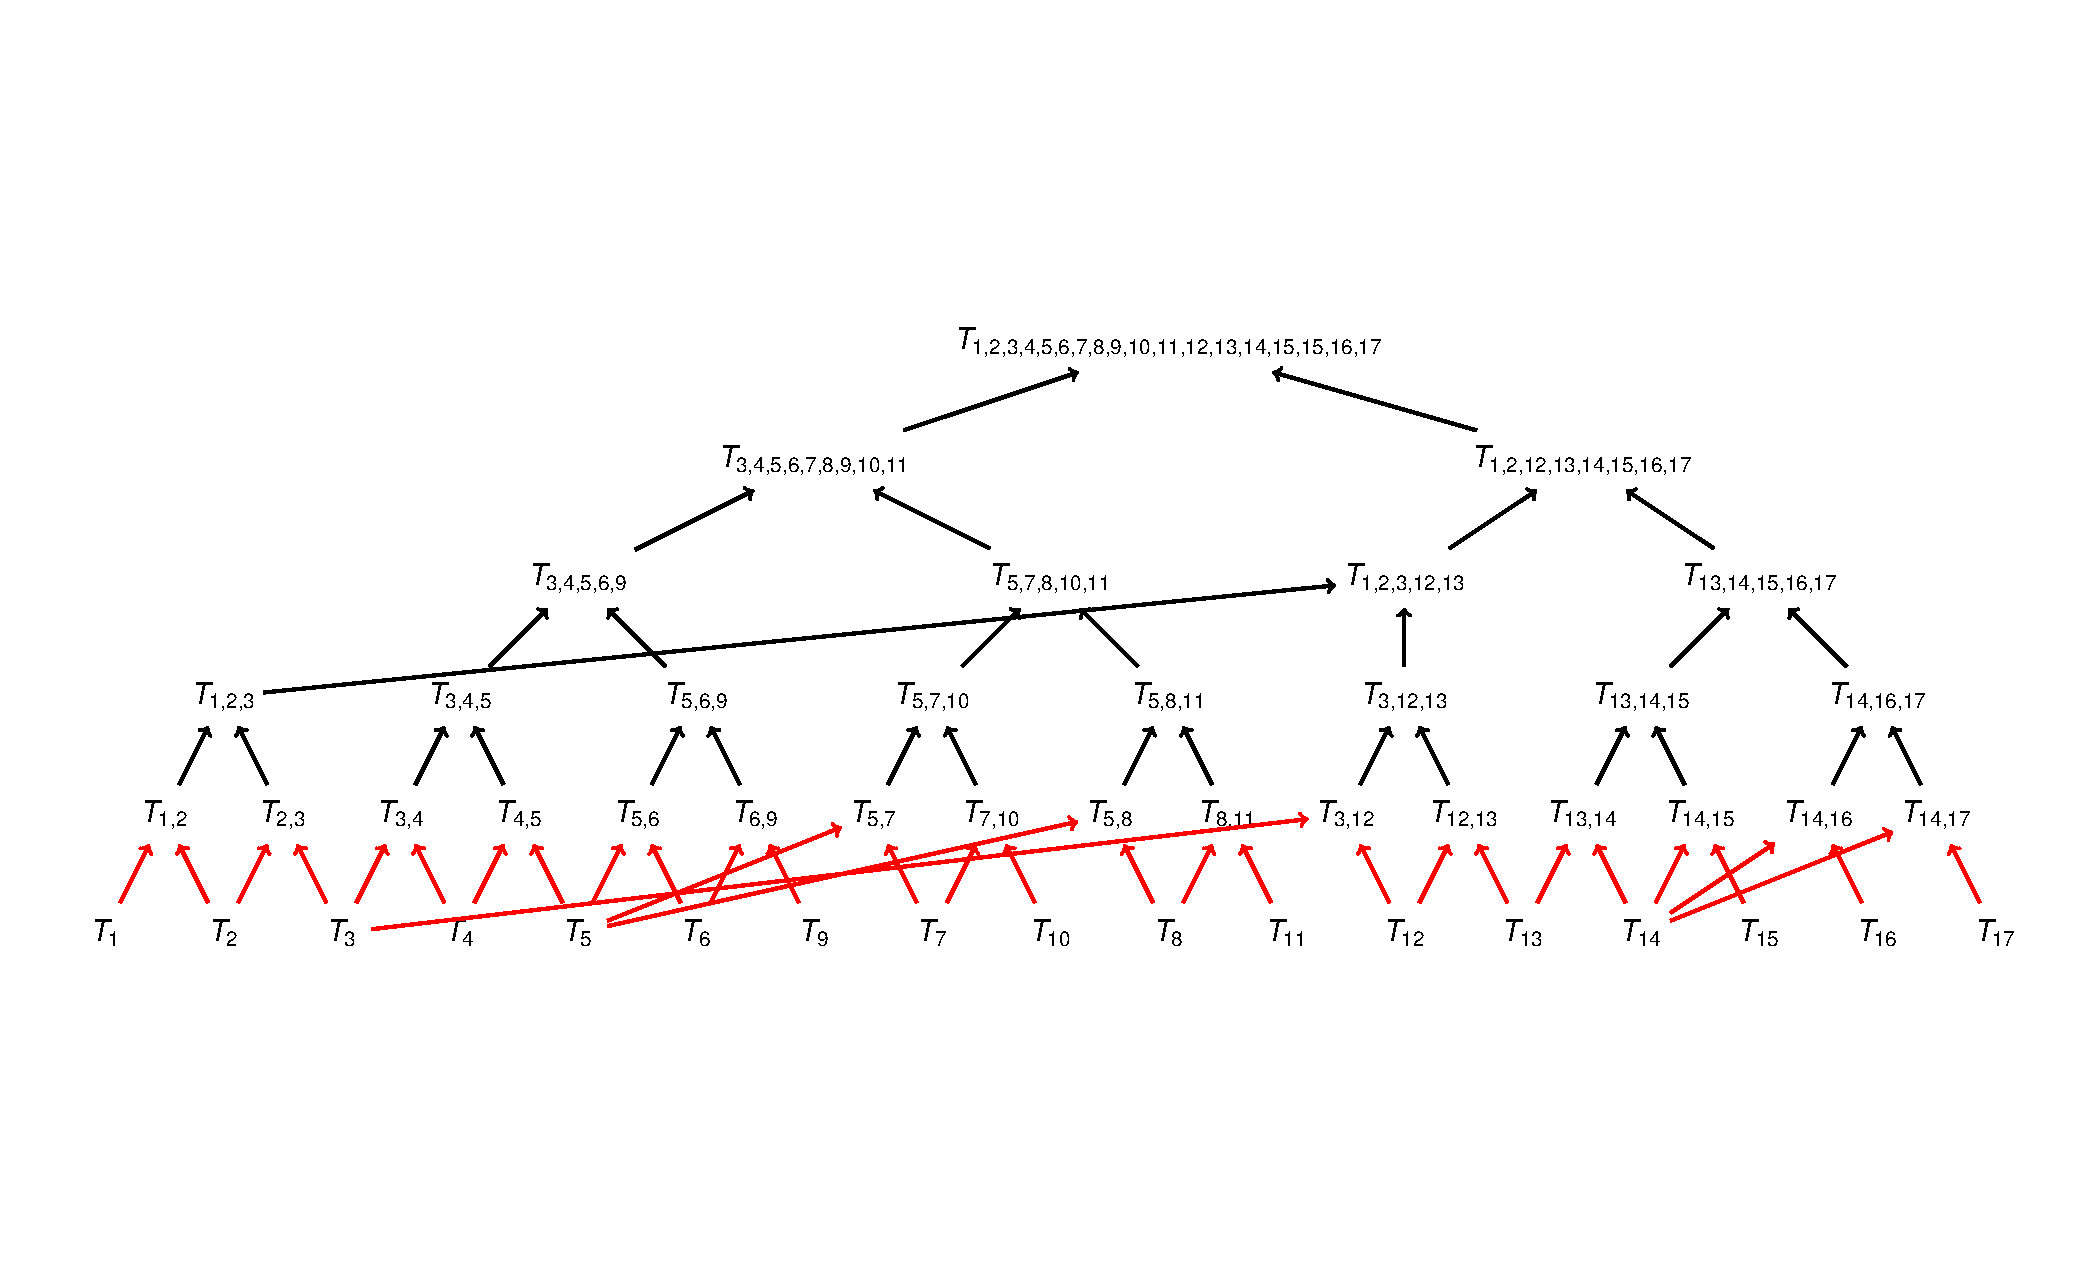
\includegraphics[scale=0.65]{figures/treemerge-fig1.pdf}
\captionsetup{singlelinecheck=off}
\caption[]{{\bf Parallel Reduction for the Generic TreeMerge.} 
It is well known that a reduction can be performed on a tree. This reduction is for subset trees $\mathcal{T} = \{T_1, T_2, \dots, T_{17} \}$ and merge guide tree $\mathcal{G}$ given by edge set: $\{(1,2), (2,3), (3,4), (4,5), (5,6), (6,9), (5,7), (7,10), (5,8), (8,11), (3,12), (12,13), (13, 14), (14, 15), (14, 16), (14, 17)\}$.
Red arrows indicate that two trees (e.g., $T_{14}$ and $T_{17}$) are given as input to a DTM method (e.g., using NJMerge). Black arrows indicate that two trees (e.g., $T_{14,17}$ and $T_{14,16}$) are merged via their shared backbone tree (e.g., using branch lengths as in TreeMerge-fast). The local merge phase is one step (red arrows), and the global merge phase takes $\log_2{(16)} = 4$ steps (black arrows). Mergers at each of these steps can be performed in an embarrassingly parallel fashion.}
\label{fig:reduction}
\end{figure}
\fillandplacepagenumber
\end{landscape}

\glsreset{blend}
\begin{figure}[!h]
\centering
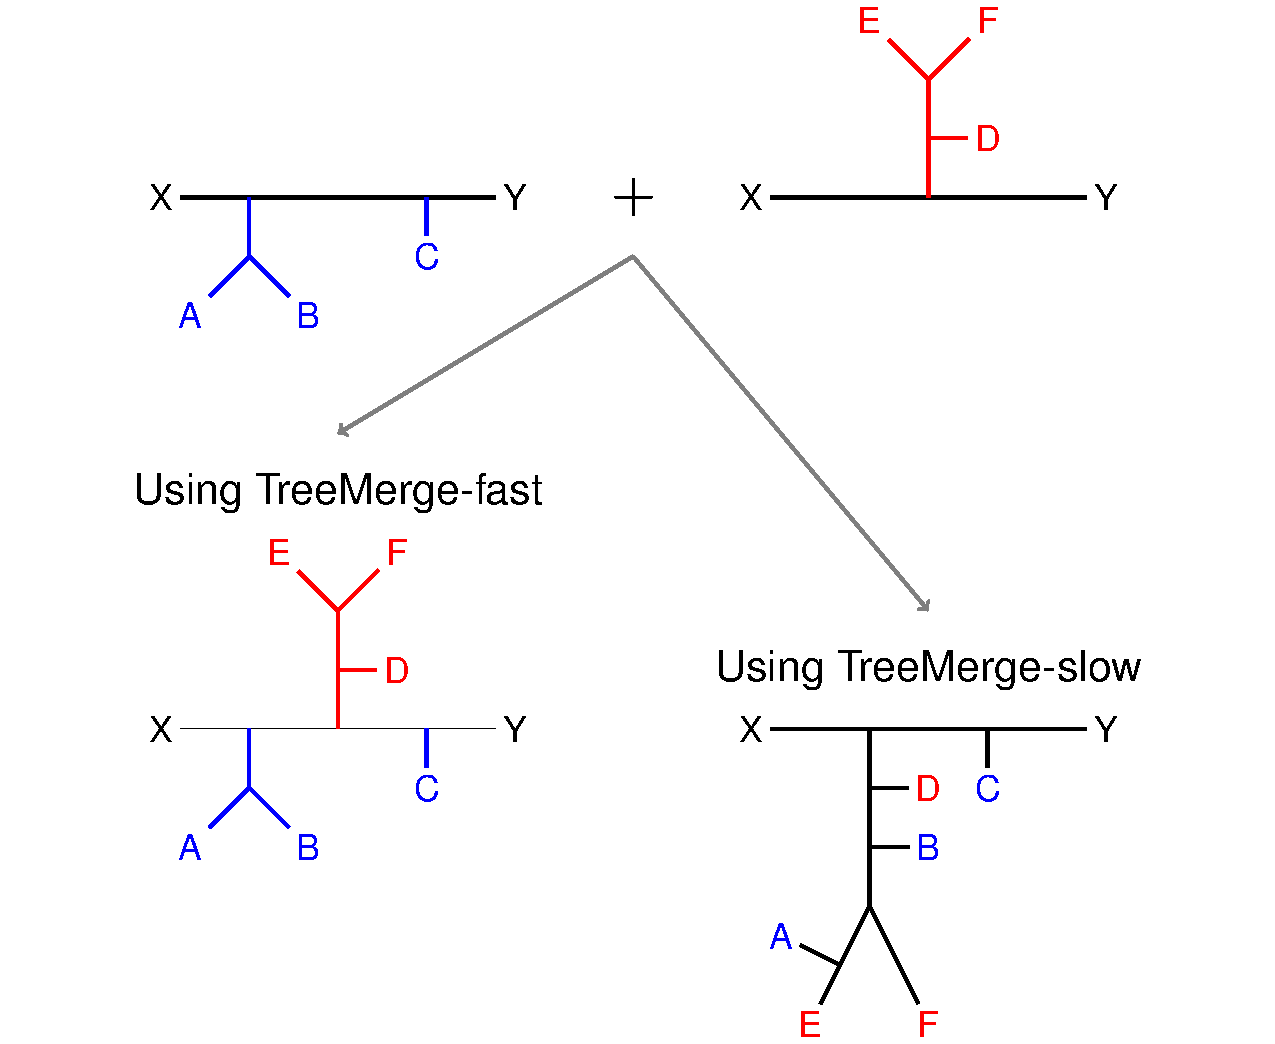
\includegraphics[width=0.9\textwidth]{figures/treemerge-fig2.pdf}
\caption{
{\bf TreeMerge-slow vs. TreeMerge-fast. }
TreeMerge-slow and TreeMerge-fast differ with respect to how they resolve edge collisions.
Consider the case where two compatible trees $T_{i,j}$ and $T_{j,k}$ are involved in a collision on edge $e = (X', Y')$ in the backbone tree $T_j$, using the notation from Section \ref{sec:treemerge}.
Select two leaves $X$ and $Y$ on opposite sides of the edge $e$ in $T_j$.
We define a constraint tree $t$ (upper left corner) by restricting $T_{i,j}$ to leaf label set $\{ x, y \} \cup \{ S(v) : v \in V_{i,j}(e) \}$, 
so the subtrees in $V_{i,j}(e)$ are given by the \gls{newick} strings: $(A,B)$ and $(C)$.
We define another constraint tree $t'$ (upper right corner) by restricting $T_{j,k}$ to leaf label set $\{ x, y \} \cup \{ S(v) : v \in V_{j,k}(e) \}$, so the one subtree in $V_{i,k}(e)$ is given by the Newick string: $(D,(E,F))$.
The goal is to produce a compatibility supertree $t^*$ for $\{ t, t' \}$ and then insert $t$ into the backbone tree $T_j$ by attaching leaf $X$ at \gls{internalnode} $X'$ and attaching leaf $Y$ at internal node $Y'$.
TreeMerge-fast builds $t^*$ by rescaling branch lengths (if necessary) so that the paths from $X$ to $Y$ in $t$ and $t'$ have the same length (as shown here); $t$ is then defined by superimposing these paths.
When resolving collisions, TreeMerge-fast does not allow \textit{\glspl{blend}}, because the subtrees in the set $V_{i,j}(e) \cup V_{j,k}(e) \cup \{X, Y\}$ must be edge separable for $t^*$.
In contrast, TreeMerge-slow builds $t^*$ by running NJMerge on the input $\big(\{t, t'\}, D|_{S(t) \cup S(t')} \big)$; this enables blending.}
\label{fig:slow-vs-fast}
\end{figure}

\begin{figure}[!h]
\centering
%\includegraphics[width=1.0\textwidth]{figures/treemerge-fig3.pdf}
	\begin{subfigure}[t]{0.45\textwidth}
	\centering
		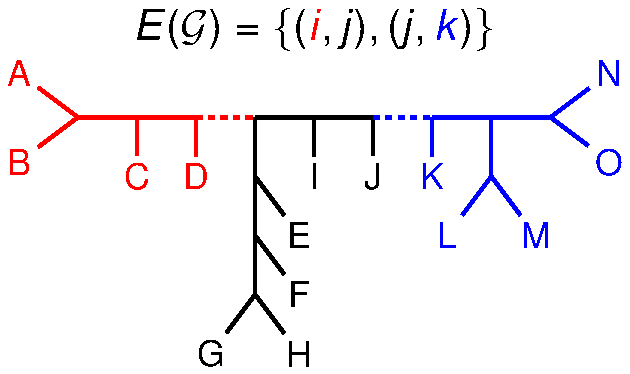
\includegraphics[width=\textwidth]{figures/treemerge-fig3a.pdf}
		~
		\caption{(a) No collisions $\{ T_{i,j}, T_{j,k} \}$} 
	\end{subfigure}
	~~~~~~~~~~
	\begin{subfigure}[t]{0.45\textwidth}
	\centering
		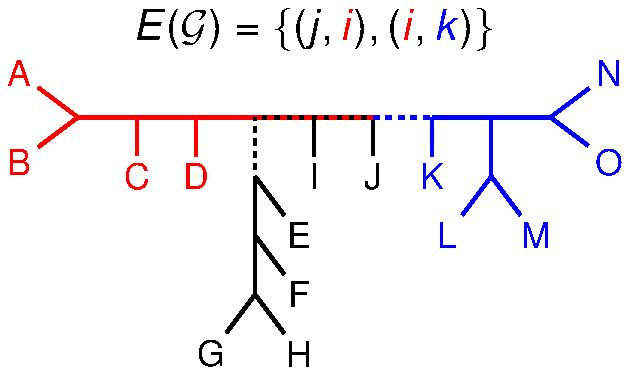
\includegraphics[width=\textwidth]{figures/treemerge-fig3b.pdf}
		~
		\caption{(b) Collisions $\{ T_{j,i}, T_{i,k} \}$} 
	\end{subfigure}

	\vspace{24pt}

	\begin{subfigure}[t]{0.45\textwidth}
	\centering
		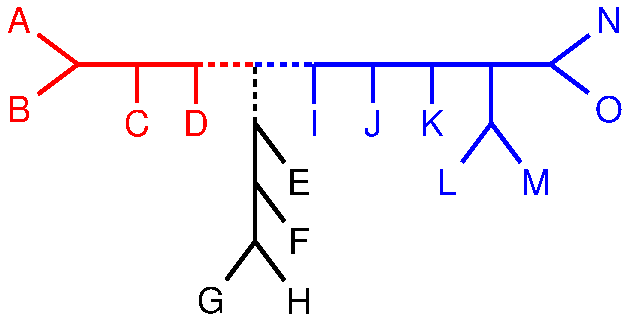
\includegraphics[width=\textwidth]{figures/treemerge-fig3c.pdf}
		~
		\caption{(c) Collision for all $\mathcal{G}$} 
	\end{subfigure}
	~~~~~~~~~~
	\begin{subfigure}[t]{0.45\textwidth}
	\centering
		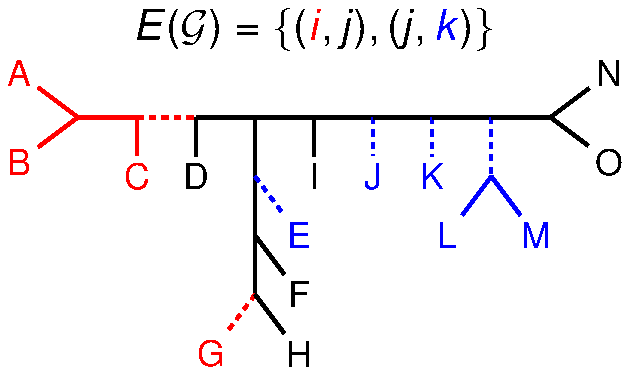
\includegraphics[width=\textwidth]{figures/treemerge-fig3d.pdf}
		~
		\caption{(d) No collisions $\{ T_{i,j}, T_{j,k} \}$} 
	\end{subfigure}
\caption{
{\bf Impact of collisions on the correctness of TreeMerge-fast. }
For each subfigure, the true tree $T$ is shown. 
Colors indicate how the leaves of $T$ have been decomposed into subsets: subset $i$, $j$, and $k$ are shown in red, black, and blue, respectively.
Suppose that subset trees $T_i$, $T_j$, or $T_k$ are correct and thus can be created by restricting $T$ to the red, black, or blue leaves, respectively.
The merge guide tree $\mathcal{G}$ indicates how the TreeMerge algorithm proceeds.
For example, in subfigure (a), $\mathcal{G}$ indicates that $\{T_i, T_j\}$ and $\{T_j, T_k\}$ are merged during the local phase. 
Again, suppose that the resulting trees are correct; therefore, $T_{i,j}$  can be created by restricting $T$ to the red and black leaves, and $T_{j,k}$ can be created by restricting $T$ to the black and blue leaves.
During the global phase, TreeMerge-fast merges $T_{i,j}$ and $T_{j,k}$ via the backbone tree $T_j$. 
Subfigure (a) shows no collisions, so TreeMerge-fast returns the correct tree.
Subfigure (b) shows a collision on the edge with bipartition $A,B,C|D$ in $T_j$, so TreeMerge-fast returns the incorrect tree; for example, TreeMerge-fast could return the tree given by Newick string: ${(\color{red} (A,B),C)},\;(((((G,H),F),E),(I,J)),{\color{blue}(K,((L,M),(O,N)))}),\;{\color{red} D})$.
Note that subfigure (b) shows the same subset decomposition as subfigure (a), but $\mathcal{G}$ is different.
Subfigure (c) shows a collision occurring regardless of $\mathcal{G}$, and TreeMerge returns the incorrect tree for this decomposition regardless of the $\mathcal{G}$; for example, TreeMerge-fast run on $\{ T_{i,j}, T_{i,k} \}$ could return ${(\color{red} ((A,B),C)},\; (((G,H),F),E),\; {\color{blue} (I,(J,(K,((L,M),(O,N)))))}, \; {\color{red} D})$.
Subfigure (d) shows no collisions, so TreeMerge-fast returns the correct tree. Unlike in the other subfigures, the subset trees $\{ T_i, T_j, T_j\}$ are not edge separable for $T$.
 }
\label{fig:collisions}
\end{figure}

\clearpage

We now provide some theoretical guarantees for TreeMerge-fast and TreeMerge-slow.

\begin{theorem}
\label{thm:treemerge-rt}
Suppose that the input $(\mathcal{T}, \mathcal{A})$ has $n$ leaf labels divided across $k$ leaf-label-disjoint trees in $\mathcal{T}$.
Then, TreeMerge-fast applied to $(\mathcal{T}, \mathcal{A})$ returns a compatibility supertree for $\mathcal{T}$ in 
 $O(nk + n^2/k + n^4/k^3)$ time if using the serial version and $O(n \log_2{k} + n^2/k^2 + n^4/k^4)$ time if using the parallel version.
TreeMerge-fast requires $O(n^2 / k)$ storage.

In contrast, TreeMerge-slow applied to $(\mathcal{T}, \mathcal{A})$ returns a compatibility supertree for $\mathcal{T}$ in $O(n^4k)$ time if using the serial version and $O(n^4)$ time if using the parallel version.
TreeMerge-slow requires $O(n^2)$ storage.
\end{theorem}

\begin{proof}
The proof that both TreeMerge-slow and TreeMerge-fast return a compatibility supertree follows from the technique for building compatibility supertrees (in the local merge phase) returning a compatibility supertree when given two leaf-disjoint trees as input and from the techniques for resolving collisions (in the global merge phase) returning a compatibility supertree when given two trees that \gls{agree} on their shared leaf label set.

For the running time analysis, we make the simplifying assumptions that each tree in $\mathcal{T}$ has exactly $n/k$ leaves and that $k-1$ is a power of two.

\emph{Local merge phase:} 
In the local merge phase, both TreeMerge-slow and TreeMerge-fast run NJMerge on input $(\{T_i, T_j\}, D^{i,j})$ for each of the $k-1$ edges in the merge guide tree $\mathcal{G}$.
All input constraint trees have $n/k$ leaves, so the local merge phase uses $O(n^2/k)$ storage.
The running time of the local merge phase is $O(n^4/k^3)$ if mergers are performed in serial and $O(n^4/k^4)$ if mergers are performed in parallel.

\emph{Extended local merge phase for TreeMerge-fast:}
TreeMerge-fast extends the local merge phase by computing branch lengths for each of the $k-1$ trees using the quadratic time and space algorithm from \cite{bryant1998rapid}. 
The running time of the extended local merge phase is then $O(n^2/k)$ if performed in serial and $O(n^2/k^2)$ if performed in parallel.

TreeMerge-fast and TreeMerge-slow implement the global merge phase differently; we discuss these methods separately using the notation from Algorithm~\ref{alg:treemerge}.

\emph{Global merge phase for TreeMerge-fast:}
At iteration $w$, TreeMerge-fast merges trees $T_{i,j}$ and $T$ using their shared backbone tree $t_B$ and branch lengths.
This is just a special case of the algorithm proposed by Bansal \cite{bansal2018linear} for Optimal Tree Completion under the \gls{RF} Distance.
This algorithm scales linearly with the number of leaf labels in the output tree, so $|S(T_{i,j}) \cup S(T)| = (w+2)n/k$.
A total of $k-2$ iterations are required, so the running time scales with $(n/k) \sum_{w=3}^k w$.
Because $\sum_{w=3}^p w$ is $O(p^2)$, the worst-case running time of TreeMerge-fast is $O(kn)$.
It is possible to perform this global merge phase in parallel via a reduction on the merge guide tree $\mathcal{G}$.
We merge trees using branch lengths in $\log_2{(k-1)}$ iterations and each iteration is $O(n)$; therefore, in the parallelized global merge
\clearpage
\noindent phase, TreeMerge-fast uses $O(n \log_2{k})$ time.

\emph{Global merge phase for TreeMerge-slow:}
At iteration $w$, TreeMerge-slow merges trees $T_{i,j}$ and $T$ using their shared backbone tree $t_B$, where $|S(T_{i,j})| = 2n/k$, $|S(T)| = (w + 1)n/k$, and $|S(t_B)| = n/k$.
There are $(w+1)n/k$ possible leaves that could be contributed to the $n/k - 3$ edges in $t_B$.
In the worst case analysis, $(w+1) n / k$ leaves are contributed to a single edge in $t_B$, so NJMerge uses $O(w^4 n^4 / k^4)$ time and $O(w^2 n^2 / k^2)$ storage.
A total of $k-2$ iterations are required, so the running time scales with $(n^4/k^4) \sum_{w=3}^k w^4$.
Because $\sum_{w=3}^p w^4$ is $O(p^5)$, the worst-case running time of TreeMerge-slow is $O(kn^4)$.
In the serialized global merge phase, TreeMerge-slow uses $O(n^4k)$ time and uses $O(n^2)$ storage.
Notably, the worst-case analysis is effectively the same as the analysis for NJMerge-2 (essentially just specifying the order of the mergers).
It is possible to perform the global merge phase in parallel via a reduction on the merge guide tree $\mathcal{G}$; the worst-case analysis is effectively the parallel version of NJMerge-2, so TreeMerge-slow requires $O(n^4)$ time.

Overall, TreeMerge-slow uses $O(n^2)$ storage and TreeMerge-fast uses $O(n^2/k)$ storage.
For the serialized versions, TreeMerge-slow runs in $O(n^4k)$ time and TreeMerge-fast runs in $O(nk + n^2/k + n^4/k^3)$ time.
For the parallelized versions, TreeMerge-slow runs in $O(n^4)$ time and TreeMerge-fast runs in $O(n \log_2{k} + n^2/k^2 + n^4/k^4)$ time.
\end{proof}

Note that while the worst-case running time of TreeMerge-slow is the same as the worst-case running time of NJMerge-2, these two methods can have very different running times in practice, for example when there are very few collisions. 
In fact, when there are zero collisions, TreeMerge-slow and TreeMerge-fast have the same running time.
That being said, it is possible for large collisions to occur; for example, if TreeMerge-slow was run on the case presented in Figure~\ref{fig:collisions}b, it would run NJMerge on two red leaves ($D$ and either $A$, $B$, or $C$), all black leaves, and all blue leaves, so basically the entire tree!

\begin{theorem}
\label{thm:treemerge-slow-correct}
If a phylogenetic tree $T^*$ is compatible with every tree in $\mathcal{T}$, and $D$ is nearly additive for $T^*$.
Then, TreeMerge-slow returns $T^*$.
\end{theorem}

\begin{proof}
Let $T_x$ and $T_y$ be two trees in $\mathcal{T}$.
NJMerge applied to $\big(\{T_x, T_y\}, D|_{S(T_x) \cup S(T_y)}\big)$ returns $T^*|_{S(T_x) \cup S(T_y)}$ by Theorem~\ref{thm:njmerge-correct}.
As TreeMerge-slow performs all its mergers using NJMerge, the result follows by induction on the number of mergers.
\end{proof}

\begin{theorem}
\label{thm:treemerge-fast-correct}
If a phylogenetic tree $T^*$ is compatible with every tree in $\mathcal{T}$, and $D$ is nearly additive for $T^*$. 
Then, TreeMerge-fast is guaranteed to return $T^*$ provided that there are no collisions during the global merge phase.
\end{theorem}

\begin{proof}
If there are no collisions during the global merge phase, TreeMerge-fast performs all of its mergers with NJMerge; the result follows by induction on the number of mergers.
\end{proof}

\subsection{Divide-and-conquer Pipelines for Phylogeny Estimation and Statistical Consistency}
We now provide some theoretical guarantees for divide-and-conquer pipelines that use either NJMerge-2, TreeMerge-slow, or TreeMerge-fast to combine subset trees; see Algorithm~\ref{alg:njmerge-divide-and-conquer}.

\begin{corollary}
When run within the divide-and-conquer framework proposed in Algorithm~\ref{alg:njmerge-divide-and-conquer}, TreeMerge-fast runs in $O(n^2)$ time if using the serial version and $O(n \log_2{n})$ time if using the parallel version.
In contrast, the parallel versions of NJMerge-2 and TreeMerge-slow run in $O(n^4)$ time, and the serial versions of NJMerge, NJMerge-2, and TreeMerge-slow run in $O(n^5)$ time.
\end{corollary}

\begin{proof}
In the divide-and-conquer framework, the input dataset of $n$ species is divided into $k$ pairwise disjoint subsets of bounded size, so $c = n/k$ and therefore $k = n/c = O(n)$.
Then, the result follows from updating the equations for worst-case running time given in Table~\ref{tab:info}.
\end{proof}

\begin{corollary}
\label{sc:treemerge-slow-sc}
NJMerge-2 and TreeMerge-slow can be used in a \gls{genetree} estimation pipeline that is statistically consistent under the \gls{GTR} model, and they can be used in a species tree estimation pipeline that is statistically consistent under the \gls{MSC} model.
\end{corollary}

The proof, which is similar to the proofs of Corollaries \ref{cor:sc-gene} and \ref{cor:sc-species}, follows easily from Theorems \ref{thm:njmerge2-rt-correct} and \ref{thm:treemerge-slow-correct}. 
To summarize, divide-and-conquer pipelines using either NJMerge, NJMerge-2, or TreeMerge-slow are statistically consistent when the method $\Phi_D$ used to estimate distances between pairs of species and the method $\Phi_T$ used to estimate constraint trees are statistically consistent under the model of interest.
These proofs of statistical consistency do not depend on the subset decomposition, the order that subsets are merged (for NJMerge-2), or the merge guide tree (for TreeMerge-slow).
Because TreeMerge-fast can fail to combine two trees correctly when collisions occur (Figure~\ref{fig:collisions}), divide-and-conquer pipelines using TreeMerge-fast are statistically consistent under a model if the probability of collisions goes to zero, as the number of samples generated under the model goes to infinity.

\begin{theorem}
\label{thm:treemerge-fast-sc}
Consider the following pipeline:
\begin{itemize}
	\item 
	Estimate a starting tree $T_0$ using method $\Phi_0$. 
	Decompose the starting tree $T_0$ into pairwise disjoint subsets $S_1, S_2, \ldots, S_k$ by removing a set $E_0$ of edges from $T_0$ such that every pair of edges in $E_0$ is separated by at least two edges in $T_0$ (e.g., Figure~\ref{fig:collisions}a). 
	Label node $v$ in $T_0$ by $i$ if $v$ is on a path between two leaves that are both in $S_i$.
	Define the merge guide tree $\mathcal{G}$ on vertex set $\{ 1, 2, \dots, k \}$ by making $i$ and $j$ adjacent in $\mathcal{G}$ if and only if there is an edge in $T_0$ whose endpoints are labeled by $i$ and $j$.
	\item Build a dissimilarity matrix $D^{i,j}$ by running method $\Phi_D$ to estimate distances between all pairs of species in the set $S_i \cup S_j$; repeat for every edge $(i, j) \in \mathcal{G}$ to produce a set $\mathcal{D}$ of dissimilarity matrices.
	\item Estimate a tree $T_i$ on subset $S_i$ using method $\Phi_T$; repeat for all $i \in \{1, 2, \dots, k\}$ to produce a set $\mathcal{T}$ of constraint trees.
\end{itemize}
Suppose that $\Phi_0$, $\Phi_D$, and $\Phi_T$ are statistically consistent under some model of evolution.
Then, as the number of independent samples generated under the model goes to infinity, the phylogenetic tree computed using TreeMerge-fast on input $(\mathcal{T},\{\mathcal{D},\mathcal{G}\})$ will converge to the true (model) tree $T^*$.
In other words, this divide-and-conquer pipeline using TreeMerge-fast is statistically consistent.
\end{theorem}
\begin{proof}
As the number of samples increases, each estimated dissimilarity matrix $D^{i,j} \in \mathcal{D}$ will converge to a matrix that is additive for $T^*|_{S(T_i) \cup S(T_j)}$, each estimated constraint tree $T_i \in \mathcal{T}$ will converge to $T^*|_{S_i}$,  and the estimated starting tree $T_0$ will converge to $T^*$.
Hence, for a large enough number of samples, the following occurs with high probability.
\begin{enumerate*}[label=(\roman*)]
	\item The deletion of edges in $E_0$ from the $T_0$ produces subsets such that the labeling of $T_0$ described above assigns each internal node with a unique label in the set $\{1, 2, \dots, k\}$; in other words, the labeling is convex on $T_0$ and thus on $T^*$.
	\item If $i$ and $j$ are adjacent in the merge guide tree $\mathcal{G}$, then $T^*|_{S_i \cup S_j}$ can be created by connecting $T_i$ and $T_j$ with an edge.
\end{enumerate*}
It is easy to see that under these conditions there will no collisions with high probability, so by Theorem~\ref{thm:treemerge-fast-correct}, TreeMerge-fast will return $T^*$ with high probability.
\end{proof}

\section{Performance Study}
\label{sec:methods}
We present the results of using TreeMerge-fast to estimate species trees on large \glspl{multi-locusdataset} simulated for the NJMerge study (Section~\ref{sec:njmerge-datasets}).
Recall that these datasets had $1\,000$ species and $1\,000$ \glspl{gene} and were characterized by two levels of \gls{ILS} (low/moderate and very high) and two data types (\glspl{exon} and \glspl{intron}).
In this study, we focus our attention on TreeMerge-fast comparing it to NJMerge and NJMerge-2.
Note that NJMerge-2 and TreeMerge-slow have the same theoretical properties for worst-case running time and statistical consistency (Table~\ref{tab:info}), but NJMerge-2 is much simpler to implement.

\begin{landscape}
\begin{table}[!h]
\captionsetup{singlelinecheck=off}
\caption[]{
{\bf Theoretical properties of NJMerge, NJMerge-2, TreeMerge-slow, and TreeMerge-fast.}
\begin{itemize}
	\item ``Can Fail?'' means that the method can, on some inputs, fail to return a tree due to algorithmic issues (rather than limited computational resources).
	\item ``Consistent?'' means that the method is statistically consistent under the GTR and MSC models when used within the divide-and-conquer pipelines described in Corollaries \ref{cor:sc-gene} and \ref{cor:sc-species}, respectively. 
	Yes$^*$ indicates that a modified divide-and-conquer pipeline is needed to ensure statistical consistency for TreeMerge-fast (Theorem \ref{thm:treemerge-fast-sc}).
	\item ``Running time'' and ``storage'' are for worst-case analysis.
	\item ``D\&C runtime'' is the running time of the method when used within the divide-and-conquer framework (Algorithm~\ref{alg:njmerge-divide-and-conquer}).
\end{itemize}
Note that TreeMerge-slow has the same worst-case running time and other properties as NJMerge-2; however, it may be faster in practice, for example when there are very few collisions.}
\label{tab:info}
\centering
\begin{tabular}{r ccccc}
\toprule
& Can Fail? & Consistent? & Running time & Storage & D\&C Runtime \\
\midrule
NJMerge & Yes & Yes & $O(n^4k)$ & $O(n^2)$ & $O(n^5)$\\
NJMerge-2 & No & Yes & $O(n^4k)$ & $O(n^2)$ & $O(n^5)$\\
Parallel NJMerge-2 & No & Yes & $O(n^4)$ & $O(n^2)$ & $O(n^4)$\\
TreeMerge-fast & No & Yes$^*$ & $O(nk + n^2/k + n^4/k^3)$ & $O(n^2/k)$ & $O(n^2)$\\
Parallel TreeMerge-fast & No & Yes$^*$ & $O(n \log_2{(k)} + n^2/k^2 + n^4/k^4)$ & $O(n^2/k)$ & $O(n\log{n})$\\
\bottomrule
\end{tabular}
\end{table}
\fillandplacepagenumber
\end{landscape}

We also perform a study similar to the NJMerge study (Section~\ref{sec:njmerge-study}), comparing TreeMerge-fast to two of the dominant species tree estimation methods: ASTRAL-III and CA-ML using RAxML.
Recall that this type of study compares running a method $\Phi_T$ within a divide-and-conquer pipeline to estimate subset trees versus running $\Phi_T$ {\em de novo} (i.e., on the full dataset).
All methods are evaluated with respect to their algorithmic failure rate (which is only relevant to NJMerge), computational failure rate (failure to complete due to insufficient computational resources), (empirical) running time, and species tree accuracy.

It is worth noting that the divide-and-conquer pipelines tested in these experiments (which were performed prior to writing Theorem ~\ref{thm:treemerge-fast-sc}) do not guarantee that the requirements for TreeMerge-fast to be statistically consistent were met.

\subsection{Divide-and-Conquer Pipelines }
\label{sec:specific-pipeline}
Divide-and-conquer pipelines require the user to specify several inputs (Algorithm~\ref{alg:njmerge-divide-and-conquer}).
We created two different pipelines: the ASTRAL-III pipeline used the estimated gene trees as input, and the RAxML pipeline used the \gls{concatenatedalignment} as input.

\paragraph{Divide-and-conquer pipeline using ASTRAL-III:}
\begin{itemize}
	\item {\em Dissimilarity matrix:} AGID matrix computed using \gls{ASTRID} version 1.4 given estimated gene trees as input
	\item {\em Starting tree:} NJ tree computed using  \gls{FastME}  version 2.1.5 on the AGID distance matrix (i.e., the \gls{NJst} tree)
	\item {\em Constraint trees:} Species trees computed using ASTRAL version 5.6.1 (i.e., ASTRAL-III) given the estimated gene trees restricted to a specific subset of species as input
\end{itemize}

\paragraph{Divide-and-conquer pipeline using RAxML:}
\begin{itemize}
	\item {\em Dissimilarity matrix: } Matrix of \glspl{log-detdistance} computed using \gls{PAUP*} version 4a163 given the concatenated alignment as input
	\item {\em Starting tree: } Greedy \gls{maximumparsimony} tree based on a random taxon addition order computed using RAxML version 8.2.12 (with SSE3 and pthreads) given the concatenated alignment as input
	\item {\em Constraint trees: } Species trees computed under the \gls{GTR+GAMMA} model of evolution using RAxML version 8.2.12 (with SSE3 and pthreads) given the concatenated alignment restricted to a specific subset of species as input
\end{itemize}

\paragraph{Subset decomposition:} 
For both pipelines, pairwise disjoint subsets of species were created by applying the \gls{centroidedgedecomposition} to the estimated starting tree $T_0$.
Note that the centroid edge decomposition does not prevent edges incident to the same node in $T_0$ from being deleted, so the requirements for TreeMerge-fast to be statistically consistent are not guaranteed to be satisfied by this pipeline (Theorem~\ref{thm:treemerge-fast-sc}).


\paragraph{Running TreeMerge-fast:}
TreeMerge-fast requires as input a merge guide tree $\mathcal{G}$, which is a tree with vertices bijectively labeled by the trees in $\mathcal{T}$.
We used the starting tree $T_0$ to construct $\mathcal{G}$ as follows.
First, we randomly selected one leaf from each tree in $\mathcal{T}$ and deleted all other leaves from $T_0$, suppressing internal nodes of degree 2; this produced a tree $T_0'$ that had one leaf for every tree in $\mathcal{T}$.
Second, we built a complete graph $\mathcal{G}_0$ with nodes labeled by the trees in $\mathcal{T}$ and edges $(T_i, T_j )$ weighted by the path distance between leaves corresponding to $T_i$ and $T_j$ in $T_0'$.
Third, we computed a minimum spanning tree $\mathcal{G}$ on $\mathcal{G}_0$ using Kruskal's algorithm \cite{kruskal1956shortest}.
This approach for producing $\mathcal{G}$ does not guarantee that requirements for TreeMerge-fast to be statistically consistent are met (Theorem~\ref{thm:treemerge-fast-sc}).
To make a fair comparison between TreeMerge-fast and NJMerge-2, the order that subset trees were merged by NJMerge-2 was equivalent to the order that subset trees were merged by TreeMerge-fast during the global merge phase.

TreeMerge-fast also requires branch lengths to be estimated on the trees produced during the local merge phase; this was accomplished by using PAUP* version 4a163 to fit least squares positive branch lengths to each of these trees using the same dissimilarity matrix from the local merge phase.

\subsection{Evaluation}
Methods were evaluated in terms of species tree error, measured as the \gls{RFerrorrate} (Equation~\ref{eq:rf-error}), and running time, measured as the wall-clock time recorded in seconds.
All computational experiments were run on the Blue Waters supercomputer, as described in Section~\ref{sec:njmerge-comp}.
We compared the time to run method $\Phi_T$ {\em de novo} (i.e., on the full dataset) to the time to run the entire divide-and-conquer pipeline; this was approximated as
\begin{equation}
	\label{eq:rt-treemerge}
	time\big(\Phi_D(X)\big) +  \sum_{T \in \mathcal{T}} time\big( \Phi_T(X|_{S(T)}) \big) + time\big( \Phi_M(\mathcal{T}, \mathcal{A}) \big)
\end{equation}
where $\Phi_M$ denotes the method to merge constraint trees using auxiliary information $\mathcal{A}$; see Algorithm~\ref{alg:njmerge-divide-and-conquer} for other notation.
Equation~\ref{eq:rt-treemerge} does not include the time to estimate starting trees, as required a few minutes compared to hundreds or thousands of minutes.

\section{Results}
\label{sec:treemerge-results}
\subsection{How does TreeMerge compare to NJMerge and NJMerge-2?}
We first evaluate the impact of running either NJMerge, NJMerge-2, and TreeMerge-fast within two divide-and-conquer pipelines (one using ASTRAL-III on subsets and one using RAxML on subsets).
First, we discuss the cases where NJMerge failed to return a tree; these failures were algorithmic rather than computational.
When ASTRAL-III was used to construct subset trees, NJMerge failed to return a tree on 0/80 datasets; however, when RAxML was used to construct subset trees, NJMerge failed to return a tree on 6/80 datasets (i.e., the failure rate was 7.5\%).
For the same analyses in the NJMerge study (Section~\ref{sec:njmerge-study}), only 2/80 datasets resulted in failures (i.e., the failure rate was 2.5\%).
The only difference between the analyses here and the ones in Section~\ref{sec:njmerge-study} is the starting tree; in this study, we used the greedy (randomized) parsimony tree from RAxML as the starting tree, whereas in the previous study, we used the NJ tree computed from the log-det distance matrix.
This finding suggests that the choice of starting tree may be a factor in whether or not NJMerge fails.
In contrast, NJMerge-2 and TreeMerge-fast completed on all datasets within the allowed time using the allowed memory.

On the replicate datasets for which all methods returned a tree, we compared NJMerge, NJMerge-2, and TreeMerge-fast in terms of species tree accuracy.
We found that NJMerge-2 produced trees with the same average error as those produced by NJMerge and that TreeMerge-fast produced trees with at most 1\% greater error on average than those produced by NJMerge (Table~\ref{tab:treemerge-s1}).

That TreeMerge-fast had similar performance compared to NJMerge and NJMerge-2 is noteworthy, as the ASTRAL-III pipeline guarantees statistical consistency for NJMerge and for NJMerge-2 but does {\em not} for TreeMerge-fast.
In particular, the centroid edge decomposition and the construction of the merge guide tree $\mathcal{G}$ do not meet the requirements described in Theorem \ref{thm:treemerge-fast-sc}.
This suggests the possibility that TreeMerge-fast might be even more accurate when used within pipelines that provide a guarantee of statistical consistency, which we note in Section \ref{sec:conclusion} as a topic for future research.

\subsection{What is the impact of using TreeMerge-fast on ASTRAL-III and RAxML?}
We now evaluate TreeMerge-fast within two divide-and-conquer pipelines (one using ASTRAL-III on subsets and one using RAxML on subsets) compared to running these methods {\em de novo}.

\paragraph{Failure rate:} 
In our experiments, ASTRAL-III and RAxML failed to complete analyses on many datasets though for different reasons.
ASTRAL-III failed to complete its analyses within 48 hours on 19/40 exon datasets and 4/40 intron datasets (i.e., the combined failure rate was 29\%); note that all of these failures occurred on datasets with very high ILS.
RAxML reported Out Of Memory (OOM) errors on 3/40 exon datasets and 39/40 intron datasets (i.e., the combined failure rate was 53\%).
In contrast, when run within divide-and-conquer pipelines using TreeMerge-fast, all analyses with ASTRAL-III and RAxML completed.
Thus, TreeMerge-fast enabled both ASTRAL-III and RAxML to complete analyses on large datasets when given only 64 GB of memory and 48 hours wall-clock time. 

Notably, the failure rate for ASTRAL-III and RAxML depended on the model condition.
RAxML failed (due to running out of memory) on more intron datasets than exon datasets.
Exon-like sequences, which evolve more slowly than intron-like sequences, had fewer distinct alignment patterns and thus could be more effectively compressed.
When the alignments could not be effectively compressed (as was the case for the intron datasets), RAxML was more likely to run out of memory.
A distributed-memory version of RAxML, called \gls{ExaML}, can be used to estimate trees when RAxML runs out of memory, provided that users have access to a distributed-memory system; in our study, we explicitly limited all methods to a single compute node, assuming users had limited computational resources.
ASTRAL-III failed (due to running longer than 48 hours) on datasets with very high ILS.
High ILS datasets are characterized by true gene trees that are topologically very different from each other and from the true species tree. 
The running time of ASTRAL-III depends on the degree of gene tree heterogeneity \cite{zhang2018astral3}, explaining why ASTRAL-III failed to complete within 48 hours on many of the high ILS datasets.

On the replicate datasets for which ASTRAL-III or RAxML completed, we compared running the methods {\em de novo} to running them within the divide-and-conquer pipeline based on TreeMerge-fast.

\paragraph{Running time:}
We found that running ASTRAL-III or RAxML within the divide-and-conquer pipeline (using TreeMerge-fast) reduced running time, often dramatically (Figures \ref{fig:astral} and \ref{fig:raxml}).
For example, when the level of ILS was very high, running ASTRAL-III within the divide-and-conquer pipeline reduced the total running time from 42 hours to 4 hours on average.
Similarly, for exon datasets, running RAxML within the divide-and-conquer pipeline reduced the total running time from 43 hours to 11 hours on average.
The time required to estimate subset trees using ASTRAL-III or RAxML typically dominated the total running time of the divide-and-conquer pipeline (with one exception: using ASTRAL-III to estimate subset trees on low ILS datasets).
Merging subset trees together with TreeMerge-fast was relatively fast, requiring no more than 46 minutes, which was between 3--11\% of the average time required to estimate subset trees using RAxML (Table~\ref{tab:treemerge-s2}).
We prototyped TreeMerge-fast (without parallelism) in Python using dendropy \cite{sukumaran2010dendropy}, so an optimized implementation (with parallelism) would produce even better results.

\paragraph{Species tree error:}
We found that whether ASTRAL-III or RAxML were run {\em de novo} or within the divide-and-conquer pipeline (using TreeMerge-fast) had little impact on species tree accuracy, with error rates differing by at most 1\% on average (Figures \ref{fig:astral} and \ref{fig:raxml}).
These effects were most pronounced for datasets with very high ILS; specifically, ASTRAL-III was more accurate (by 1\% on average) when run {\em de novo}, whereas RAxML was less accurate (by 1\% on average) when run {\em de novo}.

\section{Discussion}
\subsection{Computational Complexity, Accuracy, and Statistical Consistency}
The proof of statistical consistency for divide-and-conquer pipelines using TreeMerge-fast depends on the techniques used to  decompose the species set into subsets and to build the merge guide tree.
In Theorem~\ref{thm:treemerge-fast-sc}, we show how this can be accomplished by estimating a starting tree on the full set of species using a statistically consistent method (e.g., a \gls{distancemethod}).
Notably, divide-and-conquer pipelines using NJMerge (Algorithm~\ref{alg:njmerge-divide-and-conquer}) also compute the subset decomposition based on a starting tree.

While the statistical consistency of divide-and-conquer pipelines using NJMerge does not depend on estimating a starting tree, there is no reason not to perform the subset decomposition in this way.
NJMerge already requires an $n \times n$ dissimilarity matrix and runs $O(n^5)$ within the divide-and-conquer pipeline, so it is slower than traditional NJ and requires the same input (plus constraint trees).
The goal of NJMerge is to improve upon the accuracy of NJ by using a highly accurate but computationally intensive method to estimate subset trees.
The effectiveness of this approach (in terms of accuracy) depends on both the model condition and the methods used to estimate subset trees, as discussed in Section~\ref{sec:njmerge-discussion}.

In contrast, TreeMerge-fast does not require an $n \times n$ dissimilarity matrix and is faster than NJ, running in $O(n \log{n})$ time instead of $O(n^3)$ time, within the divide-and-conquer pipeline. 
FastME, which builds a tree from a dissimilarity matrix in $O(n^2\log{n})$ time, could be used instead of NJ, but even so, the running time of the divide-and-conquer pipeline using TreeMerge-fast will be dominated by the time to estimate a starting tree as well as the time to perform preprocessing (discussed in the next section).

For users who are willing to forgo the guarantee of statistical consistency, the first step (of building a merge guide tree and subset decomposition) could be performed using less computationally intensive techniques (especially if these techniques are highly accurate in simulation studies).
This opens up many avenues for algorithm design, and of course, determining whether these new techniques enable pipelines to be provably statistically consistent is another exciting avenue of future research.
Other algorithmic developments may aid in this endeavor; for example, combining divide-and-conquer with iteration has been used successfully to improve robustness to the initial subset decomposition in a related application: co-estimating an MSA and ML (gene) tree \cite{Liu2009rapid-sate, liu2012very-sate2, nelesen2012dactal, mirarab2015pasta}.
Iteration seems likely to be useful in the context of TreeMerge, as large collisions (i.e., collisions where TreeMerge-slow would run NJMerge on a large number of species) may indicate that starting over with a new subset decomposition and merge guide tree is necessary.

\subsection{Computational Requirements of Species Tree Estimation Pipelines} 
Many biological studies (e.g., \cite{wickett2014phylo,prum2015comprehensive}) have analyzed multi-locus datasets using ASTRAL and RAxML, so differences in their computational requirements are of interest.
The timings we report for ASTRAL-III and RAxML are {\em not} directly comparable, because the ASTRAL-III timings do not include the time required for gene tree estimation.
Using the same experimental set-up (a single Blue Waters compute node with 64 GB of memory and 16 floating-point cores), FastTree-2 took $3.6$ hours on average to estimate  $1\,000$ gene trees for datasets with  $1\,000$ species (Supplementary Tables S4 and S5 in \cite{molloy2019statistically}), so in our study the amount time spent estimating  $1\,000$ gene trees was small in comparison to the amount of time spent running ASTRAL-III on datasets with very high ILS (42 hours on average).
However, the time required for gene tree estimation can vary greatly, depending on the method used and the analysis performed (e.g., analyses that search from multiple starting trees or perform \gls{non-parametricbootstrapping} will be more computationally intensive).

It is possible that the bulk of the time could be spent estimating gene trees, but in some cases with very large numbers of species, the {\em entire} species tree estimation pipeline (which includes gene tree estimation) could be sped up by using TreeMerge-fast.
Such a pipeline would proceed as follows.
\begin{enumerate}
	\item Define pairwise disjoint subsets $S_1, S_2, \dots, S_k$ of species and a merge guide tree $\mathcal{G}$.
	\item Compute $\mathcal{T} = \{T_1, T_2, \dots, T_k\}$ and $\mathcal{D} = \{ D^{i,j} : (i,j) \in \mathcal{G} \}$ as follows.
	\begin{itemize}
		\item Root $\mathcal{G}$ at the node labeled 1 (i.e., the node corresponding to subset $S_1$). 
		\item For every edge $e = (i,j)$ in a preorder traversal of ${G}$:
		\begin{itemize}
			\item For each gene $g = \{1, 2, \dots, m\}$:
				\begin{itemize}
				\item Estimate an \gls{MSA} $A_g^{i,j}$ on species set $S_i \cup S_j$.
				\item Estimate an \gls{ML} gene tree $P_g^{i,j}$ from $A_g^{i,j}$.
				\end{itemize}
		\end{itemize}
		\begin{itemize}
		\item Compute the AGID distance matrix $D^{i,j}$ from $\mathcal{P}^{i,j} =  \{ \mathcal{P}_g^{i,j} : g \in \{1, \dots, m\}\}$.
		\item Estimate a constraint tree $T_j$ from $\{ P|_j : P \in \mathcal{P}^{i,j} \}$ using ASTRAL.
		\end{itemize}
		\item Estimate constraint tree $T_1$ on $\mathcal{P}^{1,j}$ such that $(1,j)$ exists in $E(\mathcal{G}$).
		\end{itemize}
	\item Run TreeMerge on the input $(\mathcal{T}, \{\mathcal{D}, \mathcal{G} \})$.
\end{enumerate}
This pipeline exploits locality at multiple levels: species trees do not need to be estimated on the full set of species, and similarly, gene trees and MSAs do not need to be estimated on the full set of species.

For users who want the guarantee of statistical consistency, the first step could be performed by using a statistically consistent method to build a starting tree $T_0$ on $S$ and then using $T_0$ to define pairwise disjoint subsets of species and a merge guide as described in Theorem~\ref{thm:treemerge-fast-sc}.
The former could be achieved by running NJ on a dissimilarity matrix $D$ of log-det distances (recall that log-det distances are statistically consistent under the MSC model). 
While this requires estimating an MSA for each gene on the full set $S$ of species, it does not require gene tree estimation on the full set of species.
This is critical as most (if not all) ML methods implement parallelism across sites in the MSA but {\em not} across species and therefore can be quite computationally intensive for very large numbers of species.
In fact, a promising direction of future research is to explore divide-and-conquer pipelines using TreeMerge-fast in the context of gene tree estimation.

\subsection{Future Studies}
Future studies should investigate the robustness of TreeMerge-fast to the subset decomposition and the merge guide tree.
Along these lines, other variations on the divide-and-conquer pipeline should be explicitly tested on a large collection of biological and simulated datasets.
In particular, datasets should be simulated under challenging but biologically realistic model conditions, including those that produce model violations when estimating gene trees and/or species trees with popular methods.
This is a condition where using TreeMerge may have an advantage, as some model assumptions may be preserved locally but not globally across a tree.
In the context of gene tree estimation, changes in GC content can provide evidence that stationarity, an assumption of \gls{SRH} models, is violated across the tree, but this model violation may be less significant locally.
In addition, the substitution rate matrix can change across branches of the tree, producing a model violation referred to as \textit{\gls{heterotachy}}. 
There is a growing body of literature surrounding heterotachy \cite{lopez2002heterotachy, jermiin2004biasing, lockhart2005heterotachy, zhou2007evaluation}, and this, in turn, has sparked the development of new methods, such as GHOST \cite{crotty2019ghost}.
These methods are more computationally intensive than traditional methods, so divide-and-conquer may be particularly beneficial in this context.

Of course, biologists not only want a tree topology, they also want estimates of uncertainty or estimates of the probability of error on each branch.
This is commonly achieved through non-parametric bootstrapping, an approach that can easily be applied in the context of divide-and-conquer pipelines using TreeMerge-fast. 
However, as discussed in Section~\ref{sec:include-discussion}, model violations can result in highly supported false positive branches, so interpreting differences between species estimated on the same biological datasets can be challenging.

Since the time of our study, there have been many new developments in divide-and-conquer phylogeny estimation. 
Most notably, Le {\em et al.} \cite{thien2019using} implemented a new algorithm for merging leaf-disjoint trees, called constrained-INC \cite{zhang2018constrained}, and evaluated it within the context of gene tree estimation and species tree estimation, finding that it achieved comparable accuracy to NJMerge. 
Constrained-INC is more computationally efficient than NJMerge, so constrained-INC instead of NJMerge could be called during the local merge phase or during the global merge phase (to resolve collisions when using TreeMerge-slow). 
Lastly, divide-and-conquer pipelines using DTM methods could be compared to traditional divide-and-conquer pipelines (e.g., Disk Covering Methods) when robust implementations become publicly available for species tree estimation.

\section{Conclusions}
\label{sec:conclusion}
We presented TreeMerge, a new technique for merging leaf-label-disjoint trees that addresses two important limitations of NJMerge: first that NJMerge can fail and second that NJMerge is slow, running in $O(n^4k)$ time, where $n$ is the number of species.
In contrast, the serial version of TreeMerge-fast runs in $O(nk)$ time and the parallel version runs in $O(n \log{k})$ time.
This running time advantage came at the expense of restricting the solution space, but in our simulation study, there was little difference between the accuracy of TreeMerge-fast and NJMerge.
Indeed, TreeMerge-fast was effective at scaling computationally intensive species tree estimation methods to large datasets.
The impact was greatest for those datasets on which ASTRAL-III or RAxML failed to complete, either due to limited running time (for ASTRAL-III) or limited memory (for RAxML).  
When using \gls{genome-scale} data, the computational requirements for ML analyses can be very large even for datasets with small numbers of species; for example, the Avian Phylogeomics Project with whole genomes for 48 birds used one TB of memory and took more than 200 CPU years to complete.
Today, we hope that DTM methods, including TreeMerge-fast, make it computationally feasible for researchers with limited resources to analyze large multi-locus datasets---{\em phylogenomics for all}.
In the future, we hope that the work here facilitates the development of highly parallel phylogeny estimation pipelines that have good empirical performance (accuracy) as well as good theoretical performance (statistical consistency).

\clearpage
\newpage

\section{Plots}
\label{sec:treemerge-plots}
This section contains the two plots presented in Section~\ref{sec:treemerge-results} Results.

\vspace{12pt}

\begin{figure}[!h]
\centering
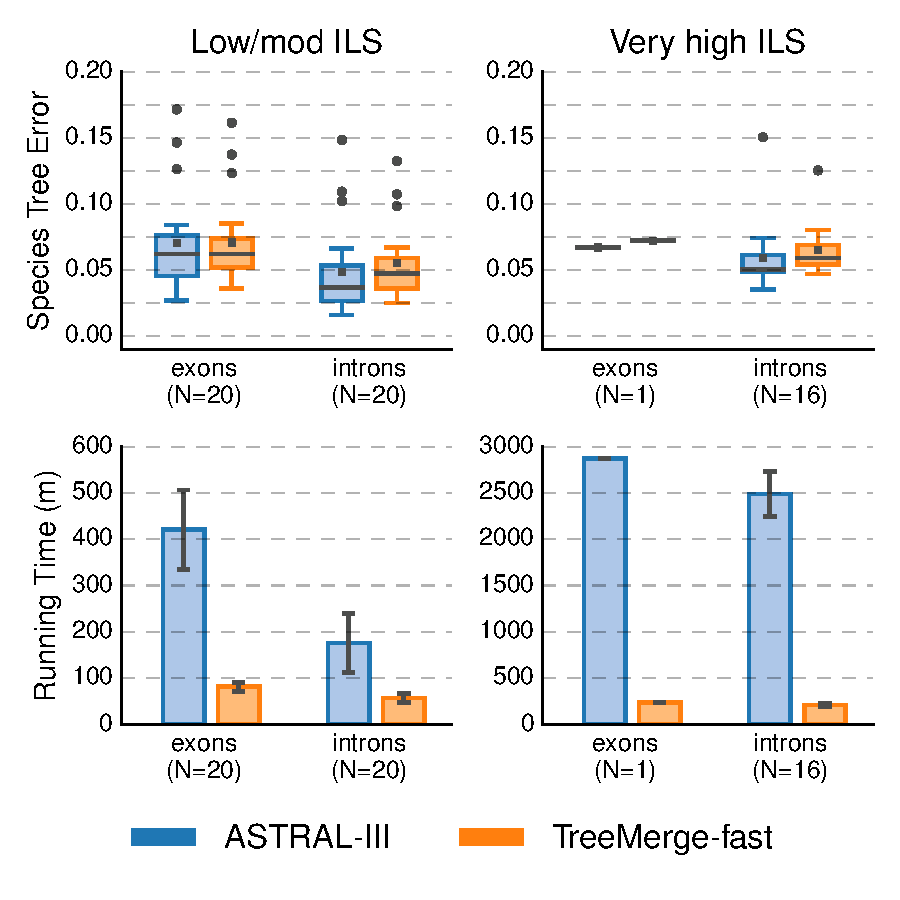
\includegraphics[width=0.8\textwidth]{figures/treemerge-fig4.pdf}
\caption{{\bf Impact of using TreeMerge-fast with ASTRAL-III. }
The top row shows species tree estimation error for datasets with  $1\,000$ species and  $1\,000$ genes. 
Gray bars represent medians, gray squares represent means, gray circles represent outliers, box plots extend from the first to the third quartiles, and whiskers extend to plus/minus 1.5 times the interquartile distance (unless greater/less than the maximum/minimum value).
The bottom row shows running time (in minutes); bars represent means, and error bars represent standard deviations across replicate datasets.
The running time of TreeMerge-fast is the time to estimate the distance matrix, to estimate each subset tree using ASTRAL-III, and to combine the subset trees using TreeMerge-fast (Equation \ref{eq:rt-treemerge}).
The number $N$ of replicates on which ASTRAL-III completed is shown on the $x$-axis; note that averages are taken across the replicates on which ASTRAL-III completed.
When ASTRAL-III did not complete, it was due to running longer than the 48-hour maximum wall-clock time.}
\label{fig:astral}
\end{figure}

%\clearpage

\begin{figure}[!h]
\centering
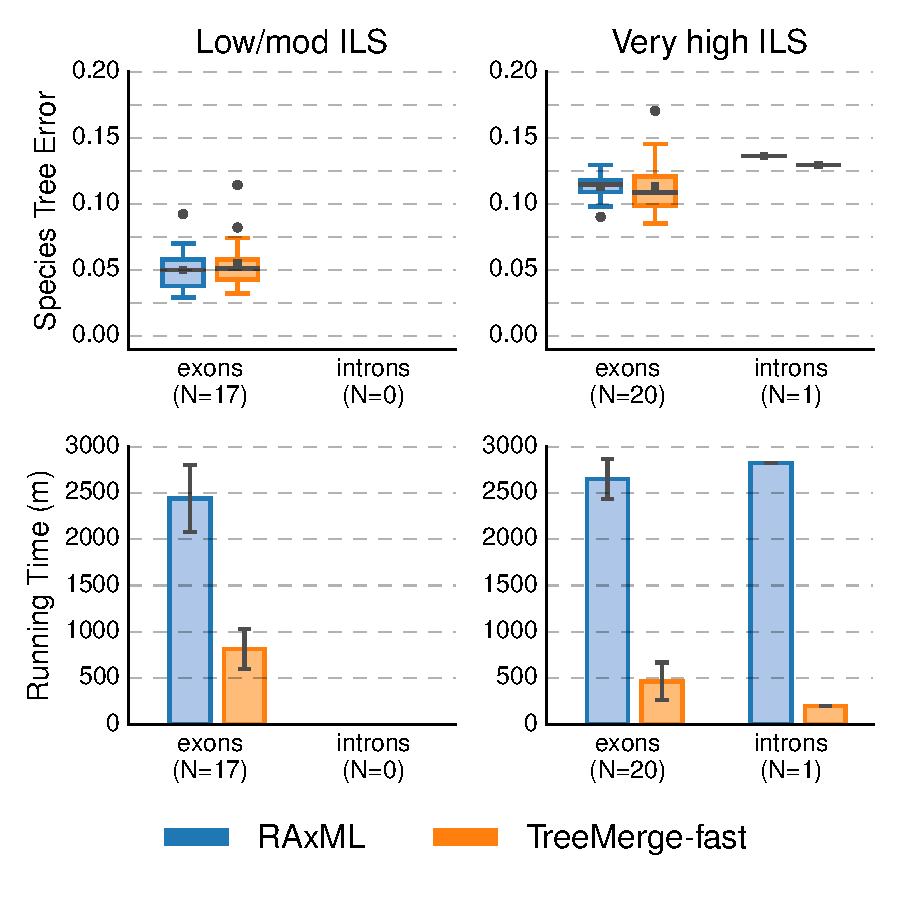
\includegraphics[width=0.8\textwidth]{figures/treemerge-fig5.pdf}
\caption{
{\bf Impact of using TreeMerge-fast with RAxML. }
The top row shows species tree estimation error for datasets with  $1\,000$ species and  $1\,000$ genes. 
Gray bars represent medians, gray squares represent means, gray circles represent outliers, box plots extend from the first to the third quartiles, and whiskers extend to plus/minus 1.5 times the interquartile distance (unless greater/less than the maximum/minimum value).
The bottom row shows running time (in minutes); bars represent means, and error bars represent standard deviations across replicate datasets.
The running time of TreeMerge-fast is the time to estimate the distance matrix, to estimate each subset tree using RAxML, and to combine the subset trees using TreeMerge-fast (Equation \ref{eq:rt-treemerge}).
The number $N$ of replicates on which RAxML completed is shown on the $x$-axis; note that averages are taken across the replicates on which RAxML completed.
When RAxML did not complete, it was due to Out Of Memory (OOM) errors; otherwise the last checkpoint written by RAxML was evaluated.
}
\label{fig:raxml}
\end{figure}

\clearpage

\section{Tables}
\label{sec:treemerge-tables}
This section contains the two tables presented in Section~\ref{sec:treemerge-results} Results.

\vspace{12pt}

\begin{table}[!h]
\caption{{\bf Species tree error for NJMerge vs. NJMerge-2 vs. TreeMerge-fast.}
A comparison of TreeMerge-fast to NJMerge and NJMerge-2 is shown below.
Species tree estimation error (average $\pm$ standard deviation; maximum error is one) is shown for datasets with  $1\,000$ species and  $1\,000$ genes.
The number of replicates on which NJMerge returned a tree is also shown, and averages are taken across the replicates on which NJMerge completed.
When NJMerge failed to return a tree, it was due to algorithmic failure (i.e., considering a siblinghood proposal to be safe when it wasn't).
}
\label{tab:treemerge-s1}
\centering
\begin{tabular}{cccccc}
\toprule
Level of & Data & Number of & NJMerge & NJMerge-2 & TreeMerge-fast \\
ILS & Type & Replicates &  &  & \\
\midrule
\multicolumn{6}{l}{\em ASTRAL-III Analysis (i.e., $M_T$ = ASTRAL-III, $M_D$ = AGID)}\\[0.5ex]
 low/mod & exon & 20 & $0.06 \pm 0.03$ & $0.06 \pm 0.03$ & $0.07 \pm 0.03$\\
 low/mod & intron & 20 & $0.05 \pm 0.03$ & $0.05 \pm 0.03$ & $0.06 \pm 0.03$\\
 very high & exon & 20 & $0.08 \pm 0.04$ & $0.08 \pm 0.04$ & $0.09 \pm 0.03$\\
 very high & intron & 20 & $0.06 \pm 0.02$ & $0.06 \pm 0.02$ & $0.06 \pm 0.02$\\[2ex]
\multicolumn{6}{l}{\em RAxML Analysis (i.e., $M_T$ = RAxML, $M_D$ = log-det)}\\[0.5ex]
 low/mod & exon & 19 & $0.04 \pm 0.02$ & $0.05 \pm 0.02$ & $0.05 \pm 0.02$\\
 low/mod & intron & 20 & $0.03 \pm 0.01$ & $0.03 \pm 0.01$ & $0.04 \pm 0.01$\\
 very high & exon & 17 & $0.10 \pm 0.01$ & $0.10 \pm 0.01$ & $0.11 \pm 0.01$\\
 very high & intron & 18 & $0.09 \pm 0.01$ & $0.09 \pm 0.01$ & $0.10 \pm 0.01$\\
\bottomrule
\end{tabular}
\end{table}

\clearpage

\begin{table}[!h]
\caption{{\bf Running time for each step in divide-and-conquer pipelines using TreeMerge-fast.}
The running time in minutes (mean $\pm$ standard deviation; maximum error is one) is given for each step in the divide-and-conquer pipeline broken down into the time to compute the distance matrix and the time to compute all subset trees and the time to merge the trees together using TreeMerge-fast (i.e., the three terms of Equation~\ref{eq:rt-treemerge}).
We do not show the time required to compute the starting tree, which required just a few minutes for both RAxML and ASTRAL-III analyses.
}
\label{tab:treemerge-s2}
\centering
\begin{tabular}{ccccc}
\toprule
Species Tree & Data & $M_D$ & $M_T$ on all & TreeMerge \\
Height & Type & & subsets &($D$, $\mathcal{T}$) \\
\midrule
\multicolumn{5}{l}{\em ASTRAL-III Analysis (i.e., $M_T$ = ASTRAL-III, $M_D$ = AGID)}\\[0.5ex]
 low/mod & exon & $1 \pm 0$ & $49 \pm 7$ & $32 \pm 5$\\
 low/mod & intron & $1 \pm 0$ & $26 \pm 7$ & $31 \pm 5$\\
 very high & exon & $1 \pm 0$  & $216 \pm 23$ & $33 \pm 6$\\
 very high & intron & $1 \pm 0$ & $178 \pm 19$ & $34 \pm 4$\\[2ex]
\multicolumn{5}{l}{\em RAxML Analysis (i.e., $M_T$ = RAxML, $M_D$ = log-det)}\\[0.5ex]
 low/mod & exon & $24 \pm 1$ & $801 \pm 228$ & $34 \pm 4$\\
 low/mod & intron & $34 \pm 3$ & $1333 \pm 301$ & $32 \pm 4$\\
 very high & exon & $23 \pm 2$ & $412 \pm 199$ & $30 \pm 5$\\
 very high & intron & $40 \pm 3$ & $752 \pm 442$ & $30 \pm 4$\\
\bottomrule
\end{tabular}
\end{table}

\clearpage



\chapter{Species Tree Estimation in the Presence of Gene Duplication and Loss with FastMulRFS}
\label{chapter:fastmulrfs}
{\em This chapter contains material perviously published in ``FastMulRFS: Fast and accurate species tree estimation under generic gene duplication or loss models'' \cite{molloy2020fastmulrfs}, which was joint work with T. Warnow.
All supplementary materials referenced in this chapter are freely available on Dryad:~\href{https://doi.org/10.1101/835553}{doi.org/10.1101/835553}.
Datasets and software commands necessary to reproduce this study are freely available on the Illinois Data Bank: \href{https://doi.org/10.13012/B2IDB-5721322_V1}{doi.org/10.13012/B2IDB-5721322\_V1}.
\emph{FastMulRFS} is freely available on Github:~\href{https://github.com/ekmolloy/fastmulrfs}{github.com/ekmolloy/fastmulrfs}.
Note that plots and tables appear at the end of this chapter in Sections~\ref{sec:fastmulrfs-plots} and \ref{sec:fastmulrfs-tables}, respectively.}
\glsreset{ILS}
\glsreset{GDL}
\glsreset{FastMulRFS}
\glsreset{MQSS}
\glsreset{DP}
\glsreset{RFS}
\glsreset{NCM}
\glsreset{HGT}
\glsreset{GTEE}
\glsreset{MRCA}
\glsreset{EPS}
\glsreset{MSA}
\glsreset{RFS}
\glsreset{ML}
\glsunset{DLCoal}
\section{Introduction}
In the previous chapters, we discussed \gls{speciestree} estimation in the presence of \gls{ILS}, where \gls{genetreeheterogeneity} is the result of genealogical relationships between \glspl{allele}.
\Gls{GDL} is another major source of \gls{genetreeheterogeneity} (one that is expected to be common in fungi \cite{butler2009evolution} and plants \cite{leebensmack2019one}).
However, most species tree estimation methods, including the ones discussed thus far in this dissertation (Section~\ref{sec:background-smethods}), are designed for \gls{orthologous} \glspl{gene}.
Because \gls{orthologydetection} is still difficult to do correctly \cite{quest2014big, lafond2018accurate, altenhoff2019inferring} and mistakes in orthology prediction can result in incorrect species trees, \gls{multi-copy} genes are often excluded from species tree estimation (e.g., \cite{wickett2014phylo, leebensmack2019one}).
Methods that can estimate species trees from \glspl{genefamily} are of increasing interest, as this would not only avoid the challenges of orthology detection but also enable the phylogenetic signal in multi-copy genes to be leveraged during species tree estimation.

Several methods have been proposed to estimate species trees from multi-copy genes.
The most well-known method explicitly based on a parametric model of GDL is probably PHYLDOG \cite{boussau2013genome-phyldog}, which uses likelihood to co-estimate the species tree and gene family trees. 
PHYLDOG is very computationally intensive and so is limited to very small datasets with 10 or so species.
Recently, De~Oliveira Martins~{\em et al.}~\cite{de2016bayesian-guenomu} proposed a Bayesian \gls{supertree} method {\em guenomu} for multi-copy gene trees.
Because {\em guenomu} requires a posterior distribution to be estimated for each gene family tree (e.g., using MrBayes \cite{ronquist2003mrbayes}) as input, it is not fast enough to use on \gls{genome-scale} datasets with 100 or more species.

Non-parametric methods are more commonly used alternatives. 
For example, \textit{\gls{GTP}} methods take a set of (estimated) gene family trees as input, and then seek a species tree that implies the minimum number of evolutionary events, such as gene duplications and gene losses.
Examples of GTP methods include DupTree \cite{wehe2008duptree}, iGTP \cite{chaudhary2010igtp}, and DynaDup \cite{bayzid2018gene}.
Since GTP is NP-hard, most of these methods operate by using hill-climbing.
DynaDup, in contrast, uses \gls{DP} to find an optimal solution within a constrained search space; this type of approach, to the best of our knowledge, was first proposed in \cite{hallett2000new} and has since been utilized for other problems (note that this is the type of approach used by \gls{ASTRAL} to solve the \gls{bipartition-constrained} \gls{MQSS} problem \cite{bryant2001constructing, mirarab2014astral}). 
Although GTP methods can be computationally intensive, they are more scalable than other approaches, and several phylogenomic studies have used GTP methods to analyze biological datasets (e.g., \cite{sanderson2007inferring, burleigh2010genome}).

Other fast approaches include supertree methods that have been adapted to work with gene family trees, referred to as \glspl{MUL-tree}.
The most well known supertree method for MUL-trees is perhaps MulRF \cite{chaudhary2014mulrf}, which attempts to find a solution to the NP-hard Robinson-Foulds Supertree problem for MUL-trees (\gls{RFS-MUL-trees}).
Although MulRF does not explicitly account for GDL, it has been shown to produce more accurate species trees than DupTree and iGTP on datasets simulated under challenging model conditions with gene tree heterogeneity due to GDL, ILS, \gls{HGT}, and \gls{GTEE} \cite{chaudhary2014assessing}.

In a very recent advance, Legried {\em et al.} \cite{legried2020polynomial} proved that
ASTRAL-multi \cite{rabiee2019multi}, an extension of ASTRAL \cite{mirarab2014astral} to address multi-allele inputs, is \gls{statisticallyconsistent} under the probabilistic model of GDL proposed by Arvestad {\em et al.} \cite{arvestad2009gene} (recall that gene trees evolve \gls{iid} within a species tree with a duplication rate and a loss rate fixed across the edges of the species tree; see Section~\ref{sec:background-gdl}).
In fact, ASTRAL-multi is the only method that has been proven statistically consistent under any GDL model.
Yet, the experimental study comparing ASTRAL-multi to three earlier species tree estimation methods, including DupTree, STAG \cite{emms2018stag}, and MulRF, showed that ASTRAL-multi had good but not exceptional accuracy.
When the duplication and loss rates were both high, ASTRAL-multi was less accurate than MulRF (although ASTRAL-multi was more accurate than STAG and typically more accurate than DupTree except when GTEE was low). 
The high accuracy of MulRF in comparison to ASTRAL-multi encouraged us to explore the optimization problem that MulRF attempts to solve.

In the remainder of this chapter, we prove that the true species tree is an optimal solution to the RFS-MUL-trees problem, provided there is no \gls{adversarialGDL} (which occurs when the pattern of \glspl{duplicationevent} and \glspl{lossevent} produces \glspl{bipartition} that are incompatible with the species tree).
This model is less restrictive than the probablistic GDL model in that it does not assume genes evolve {\em i.i.d.}~(similar to the \gls{NCM} model) but is more restrictive in that it prohibits adversarial GDL.
However, we conjecture that adversarial GDL will occur with sufficiently low probability so that an exact solution to the RFS-MUL-trees problem will be statistically consistent for reasonable duplication and loss probabilities.
This result is enabled by proving that, when solving the RFS-MUL-trees problem, any input set of MUL-trees can be replaced by a set of \gls{singly-labeled} trees.
By combining this reduction technique with DP within a constrained search space, we develop a new method, \textit{\gls{FastMulRFS}}.
As we will show, FastMulRFS is statistically consistent under a generic GDL model that prohibits adversarial GDL.

Lastly, we compare FastMulRFS to ASTRAL-multi, DupTree, and MulRF on datasets simulated under the \gls{DLCoal} model with varying levels of GDL, ILS, and GTEE. 
As we will show, FastMulRFS is generally more accurate than  DupTree and ASTRAL-multi and ties for most accurate with MulRF.
In addition, FastMulRFS is much faster than MulRF and ASTRAL-multi and ties for fastest with DupTree.
The improvement in performance over ASTRAL-multi is the most important result, as ASTRAL-multi is the only other method to date that has been proven statistically consistent under a probabilistic GDL model.
In summary, FastMulRFS is a fast method for species tree estimation that does not require reliable orthology detection and outperforms the leading alternative methods (even under conditions for which FastMulRFS is not yet established to be statistically consistent).

\section{Approach}
\label{sec:fastmulrfs-approach}
\glsreset{RFS-MUL-trees}
\glsreset{FastMulRFS}
We begin by extending some of the terminology and definitions from Sections~\ref{sec:background-tree}---\ref{sec:background-supertrees} to MUL-trees.
Recall that a {\em phylogenetic tree} $T$ is defined by the triplet $(t, S, \phi)$, where $t$ is a tree, $S$ is a set of labels, and $\phi: L(t) \rightarrow S$ assigns labels to the leaves of $t$.
If $\phi$ is a bijection, we say that $T$ is singly-labeled; otherwise, we say that $\phi$ is multi-labeled or equivalently that $T$ is a MUL-tree.
Recall that deleting an edge $e$ but not its endpoints from $T$ produces two  subtrees $t_A$ and $t_B$, defining two label sets: $A  = \{ \phi(l) : l \in L(t_A) \}$ and $B = \{ \phi(l) : l \in L(t_B) \}$.
When $T$ is singly-labeled, every edge $e \in E(T)$ splits the leaf labels into two sets $A$ and $B$ such that $A \cap B = \emptyset$; this does not hold when there are two leaves in $T$ with the same label.
Lastly, recall that the \gls{RF} distance (i.e., the edit distance under \gls{contraction} and \gls{refinement} operations) between two singly-labeled trees on the same label set can be computed as the bipartition distance (Theorem~\ref{thm:rf}).
Theorem~\ref{thm:rf} does not hold when one or both trees is a MUL-tree.

\subsection{Robinson-Foulds Supertree problem for MUL-trees}
To present the RF supertree problem for MUL-trees, we need three additional definitions
\clearpage
\noindent from Ganapathy {\em et al.} \cite{ganapathy2006pattern} and Chaudhary {\em et al.} \cite{chaudhary2013inferring}.

\begin{definition}[Full Differentiation]
\label{defn:diff}
We say that $M' = (m, S', \phi')$ is a \emph{\gls{fulldifferentiation}} of MUL-tree $M = (m, \phi, S)$ if $\phi' : L(m) \rightarrow S'$ is a bijection. In other words, $M'$ is a singly-labeled version of $M$.
\end{definition}

\begin{definition}[Mutually Consistent Full Differentiations]
\label{defn:mcsd}
Let $M_1' = (m_1, S', \phi_1')$ and $M_2' = (m_2, S', \phi_2')$ be full differentiations of MUL-trees $M_1 = (m_1, S, \phi_1)$ and $M_2  = (m_2, S, \phi_2)$, respectively.
For $i=1,2$, we define $R_i(s) \subseteq S'$ to be the set of labels given to the leaves in $M_i'$ that are labeled $s$ in $M_i$.
We say that $M_1'$ and $M_2'$ are \emph{\glspl{MCFD}} of $M_1$ and $M_2$ if $R_1(s) = R_2(s)$ $\forall s \in S$.
\end{definition}

Ganapathy {\em et al.} \cite{ganapathy2006pattern} showed that if $M_1$ and $M_2$ are both MUL-trees, then their RF distance can be computed as 
\begin{equation}
	\label{eq:mulrf}
	MulRF(M_1, M_2) := \\
	\min\{ RF(M_1', M_2') : M_1', M_2' \text{ are MCFDs of } M_1, M_2 \}
\end{equation}
which implies an exponential-time algorithm for computing the RF distance between two MUL-trees \cite{ganapathy2006pattern},
Later, this problem was proven to be NP-complete by Chaudhary {\em et al.} \cite{chaudhary2013inferring}.

Chaudhary {\em et al.} \cite{chaudhary2013inferring} also introduced a special case, where one of the two MUL-trees has the following property: every leaf with the same label is grouped together in a \gls{polytomy} that is separated by an edge from the rest of the tree.
A MUL-tree with this property can be viewed as an extended version of a singly-labeled tree.

\begin{definition}[Extended Version]
\label{defn:extd}
Let $T = (t, S, \phi_T)$ be a singly-labeled tree, let $M = (m, S, \phi_M)$ be a MUL-tree, and let $k(s)$ be the number of leaves with label $s$ in $M$.
The \emph{\gls{extendedversion}} of $T$ with respect to $M$, denoted $Ext(T,M)$, is created by attaching $k(s)$ new leaves to the leaf labeled $s$ in $T$, assigning label $s$ to each of these new leaves, and then repeating this process for all $s \in S$.
\end{definition}

Chaudhary {\em et al.} \cite{chaudhary2013inferring} showed that the RF distance between a MUL-tree $M$ and an extended version of a singly-labeled tree $Ext(T,M)$ can be computed in polynomial time.
Based on this result, they proposed the Robinson-Foulds Supertree problem for MUL-trees (RFS-MUL-trees).

\begin{definition}[Robonsin-Foulds Supertree Problem for MUL-trees]
Let $\mathcal{T}$ be a set of MUL- trees.
If a tree $T^*$ on label set $S = \bigcup_{M \in \mathcal{T}} S(M)$ is in the set
\begin{equation}
    \label{eq:mulrfsp}
    \sum_{M \in \mathcal{P}} RF(Ext(T|_{S(M)}, M)', M')
\end{equation}
then we say that $T^*$ is an \emph{\gls{RFS-MUL-trees}} supertree for $\mathcal{T}$.
\end{definition}

Note that when $\mathcal{P}$ is a profile of singly-labeled trees, then the RFS-MUL-trees problem is equivalent to the \gls{RFS} problem.

\vspace{12pt}

\begin{figure}[!h]
	\centering
	%\includegraphics[width=\textwidth]{figures/fastmulrfs-fig1.pdf}
	\begin{subfigure}[t]{0.36\textwidth}
	\centering
		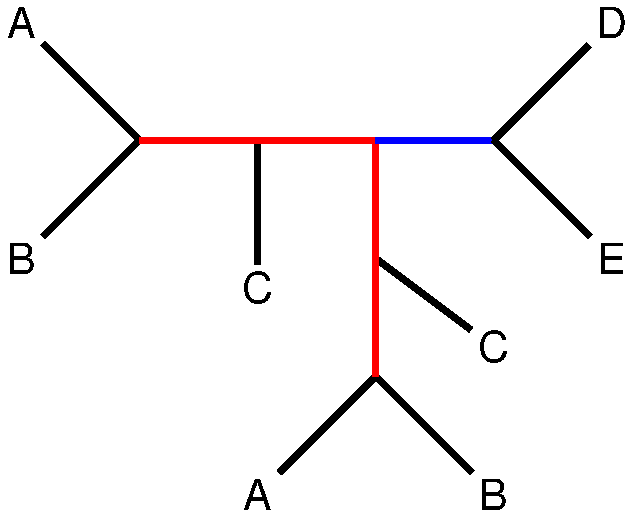
\includegraphics[width=\textwidth]{figures/fastmulrfs-fig1b.pdf}
		~
		\caption{(b) Mul-tree $M$}
	\end{subfigure}
	~~~~~~~~~~~~~~~
	\begin{subfigure}[t]{0.432\textwidth}
		\centering
		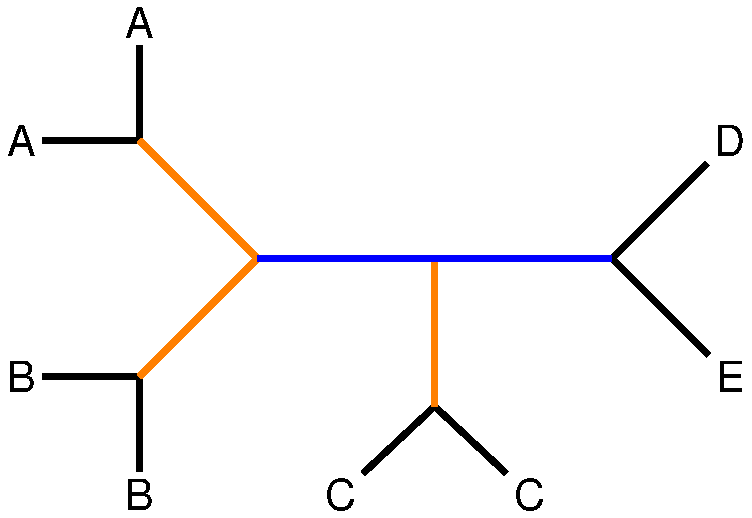
\includegraphics[width=\textwidth]{figures/fastmulrfs-fig1c.pdf}
		~
		\caption{(c) $Ext(T,M)$}
	\end{subfigure}
	
	\vspace{24pt}

	\begin{subfigure}[t]{0.3\textwidth}
		\centering
		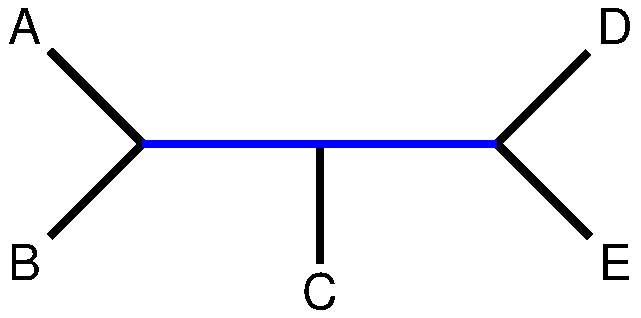
\includegraphics[width=\textwidth]{figures/fastmulrfs-fig1a.pdf}
		~
		\caption{(a) Singly-labeled tree $T$}
	\end{subfigure}
	~~~~
	\begin{subfigure}[t]{0.3\textwidth}
		\centering
		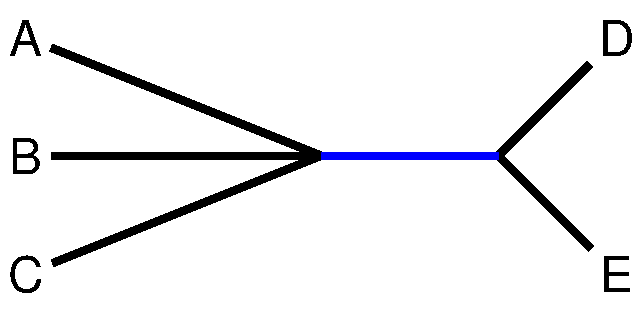
\includegraphics[width=\textwidth]{figures/fastmulrfs-fig1e.pdf}
		~
		\caption{(e) $\mathcal{R}(\mathcal{X}(M))$}
	\end{subfigure}
	~~~~
	\begin{subfigure}[t]{0.3\textwidth}
		\centering
		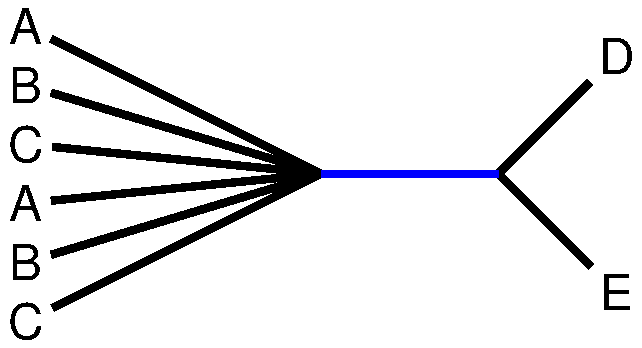
\includegraphics[width=\textwidth]{figures/fastmulrfs-fig1d.pdf}
		~
		\caption{(d) $\mathcal{X}(M)$}
	\end{subfigure}
	\caption{
	{\bf Reduction of the RFS-MUL-trees problem to the RFS problem.}
	Subfigure (a) shows a candidate RFS-MUL-trees supertree $T$ for a set $\mathcal{P}$ of MUL-trees, and subfigure (b) shows a MUL-tree $M$ in ${P}$; note that both $T$ and $M$ are on the same label set $S = \{A, B, C, D, E\}$.
    To compute the RF distance between $T$ and $M$, we build the extended version of $T$ with respect to $M$ (Definition~\ref{defn:extd}), producing $Ext(T,M)$, as shown in subfigure (c).
    The trivial edges in $Ext(T,M)$ (shown in orange) exist in {\em any possible} singly-labeled, binary tree on $S$, so these edges do not impact the solution to the RFS-MUL-trees problem.
    Similarly, the edges in MUL-tree $M$ that are shown in red cannot exist in an extended version of {\em any possible} singly-labeled, binary tree on $S$, so these edges do not impact the solution to the RFS-MUL-trees problem.
   We contract all internal edges in $M$ with the property that there are at least two leaves, one on either side of the edge, with the same label; this produces $\mathcal{X}(M)$, as shown in subfigure (d).
    Furthermore, because all leaves with the same label are now on the same side of {\em every} edge in $\mathcal{X}(M)$, we can delete all but one leaf with each label; this produces $\mathcal{R}(\mathcal{X}(M))$, as shown in subfigure (e).
    The resulting tree is a non-binary, singly-labeled tree on $S$, so we can compute the RF distance between $T$ and $\mathcal{R}(\mathcal{X}(M))$ using Equation~\ref{eq:rf}.
    These observations are formalized in Lemma~\ref{lem:mulrf2}.
    }
	\label{fig:1}
\end{figure}

\subsection{Reducing from MUL-trees to singly-labeled trees}
\label{sec:reduction}
We simplify the RFS-MUL-trees problem by providing an alternative proof that the RF distance between between a singly-labeled tree $T$ and a MUL-tree $M$ can be computed (up to a constant factor that does not depend on $T$) in polynomial time by reducing the MUL-trees to a set of singly-labeled trees; see Figure \ref{fig:1} for intuition behind this proof.

To begin, we define two transformations that can be applied to a MUL-tree $M = (m, S, \phi)$ or to its full differentiation $M' = (m, S', \phi')$ by using the function $f: S' \rightarrow S$ with the property that $f(\phi'(l)) = \phi(l)$ for all $l \in L(m)$.

\begin{definition}[Contracted Version]
\label{defn:conv}
The \emph{\gls{contractedversion}} of $M$, denoted $\mathcal{X}(M)$, is created by contracting every \gls{internaledge} $e$ with the property that there are at least two leaves, one on either side of the edge, with the same label.
Similarly, the contracted version of $M'$, denoted $\mathcal{X}(M')$, is created by contracting every internal edge $e$ with $\pi(e) = A|B$ such that $f(A) \cap f(B) \neq \emptyset$.
\end{definition}

\begin{definition}[Reduced Version]
\label{defn:redv}
If all leaves with species label $s$ are on the same side of {\em every} internal edge in $E(M)$, then they can be represented by a single leaf labeled $s$.
The \emph{\gls{reducedversion}} of $M$ or $M'$, denoted $\mathcal{R}(M)$ or $\mathcal{R}(M')$, respectively, is created as follows. 
For every $s \in S$ with the aforementioned property, delete all but one of the leaves in the set $\{ f(\phi'(l)) = \phi(l) = s : l \in L(m) \}$ (suppressing \glspl{internalnode} of degree 2) and relabel the remaining leaf $s$.
\end{definition}

It is easy to see that $\mathcal{R}(\mathcal{X}(M'))$ is a singly-labeled tree that is isomorphic to $\mathcal{R}(\mathcal{X}(M))$, because after applying the function $\Sigma$ to either $M'$ or $M$, all the leaves with species label $s$ will be on the same side of every edge and thus can be replaced by a single leaf with species label $s$ by applying the function $\mathcal{R}$. 
This observation holds for all $s \in S$.

\begin{lemma}
\label{lem:mulrf2}
Let $T$ be an unrooted, singly-labeled, and \gls{fullyresolved} tree on label set $S$, 
let $M = (m, S, \phi)$ be an unrooted MUL-tree, and
let $Ext(T,M)'$ and $M' = (m, S', \phi')$ be MCFDs of $Ext(T,M)$ and $M$, respectively.
Then,
\begin{equation}
	\label{eq:mulrf2}
	RF(Ext(T,M)', M') = RF(T, M_X) + K
\end{equation}
where $M_X = \mathcal{R}(\Sigma(M))$ and $K$ is a constant that does not depend on the \gls{topology} of the singly-labeled tree $T$ on $S$.
\end{lemma}
\begin{proof}
Let $f: S' \rightarrow S$ be a function with the property that $f(\phi'(l)) = \phi(l)$ for all $l \in L(m)$.
Now we define the following bipartition sets.
\begin{align}
	X &= \{  A|B \in Bip(M') : f(A) \cap f(B) \neq \emptyset \} \\
	R &= \{ A|B \in Bip(M') \setminus X : |A| > 1, |B| > 1, \text{ and either } |f(A)| = 1 \text{ or } |f(B)| = 1 \}
\end{align}
It is easy to see that $X$ contains bipartitions that {\em cannot exist} in $Bip(Ext(T,M)')$ for any singly-labeled tree $T$ on $S$ and that $R$ contains bipartitions that {\em must exist} in $Bip(Ext(T,M)')$ for any singly-labeled tree $T$ on $S$.
(note that edges that induce bipartitions in the set $X$ are colored red in Figure~\ref{fig:1}b and edges that induce bipartitions in the set $R$ are colored orange in Figure~\ref{fig:1}c.)
Let $E'$ denote $Ext(T,M)'$. Then,
\begin{align}
| Bip(E') \cap Bip(M') | &= | Bip(E') \cap Bip(\mathcal{X}(M')) | \\
	&= | Bip(\mathcal{R}(E')) \cap Bip(\mathcal{R}(\mathcal{X}(M'))) | + | R | + |L(m)| - | S | \nonumber  \\
	&= | Bip(T) \cap Bip(M_X) | + | R | + |L(m)| - | S | \nonumber \\
	&= 0.5 \big[ | E(M_X)| + | E(T) | - RF(T, M_X) \big] + | R | + |L(m)| - | S | \nonumber \\
	&= 0.5 \big[ | E(M_X)| + 2 | S | - 3 - RF(T, M_X) \big] + | R | + |L(m)| - | S | \nonumber \\
	&= 0.5 \big[ | E(M_X) | - 3 - RF(T, M_X) \big] + | R | + |L(m)| \nonumber
\end{align}
Let $c$ be the number of species in $S(M)$ that have multiple copies (i.e., $c = | \{ s \in S(M) \}|$). 
Then,
\begin{align}
RF(E', M') &= |E(E') | + |E(M')| - 2| Bip(E') \cap Bip(M') | \\
&= \big( |S| - 3 + c + |L(m)|  \big)  + | E(m) | - 2| Bip(E') \cap Bip(M') | \nonumber \\
&= RF(T, M_X) + |S| + c + | E(m) | - | E(M_X) | - 2 |R| - |L(m)| \nonumber
\end{align}
where $S$, $c$, $E(m)$, $E(M_X)$, $R$, and $L(m)$ are independent of $T$.
\end{proof}

In Lemma~\ref{lem:mulrf2}, we show that $MulRF(Ext(T,M),M)$ can be computed in polynomial time, because computing $RF(Ext(T,M)',M')$ does not depend on the MCFDs of $Ext(T,M)$ and $M$. 
In addition, we show that the RF distance between $Ext(T,M)$ and $M$ can be computed (up to a constant factor that does not depend on the topology of a singly-labeled tree $T$ on $S$) by simply transforming $M$ into a (potentially \gls{unresolved}) singly-labeled tree on $S$ and computing its RF distance from $T$.

The following theorem easily follows from Lemma~\ref{lem:mulrf2}.

\begin{theorem}
\label{thm:equal}
Let $\mathcal{P}$ be a set of unrooted MUL-trees, let $\mathcal{P}_X = \{ \mathcal{R}(\mathcal{X}(M)) : M \in \mathcal{P} \}$, and let $T$ be an unrooted, singly-labeled, and fully resolved tree on label set $S = \bigcup_{M \in \mathcal{P}} S(M)$.
Then, $T$ is an RFS-MUL-trees supertree for $\mathcal{P}$ if and only if $T$ is an RF supertree for $\mathcal{P}_X$.
\end{theorem}

\begin{definition}[Valid and Invalid Bipartitions]
\label{def:valid}
Let $M = (m, S, \phi)$ be an unrooted MUL-tree.
Suppose that deleting an edge $e$ but not its endpoints from $M$ produces two subtrees $m_A(e)$ and $m_B(e)$, defining the label sets: $A  = \{ \phi(l) : l \in L(M_A) \}$ and $B = \{ \phi(l) : l \in L(M_B) \}$.
If $A\cap B = \emptyset$, we say that $e$ induces a \emph{\gls{validbipartition}} and allow $\pi(e) = A|B$ to be contributed to the set $Bip(M)$.
If $A \cap B \ne \emptyset$, we say that $e$ induces an \emph{\gls{invalidbipartition}} and do \emph{not} allow $\pi(e) = A|B$ to be contributed to the set $Bip(M)$; alternatively, we say that $e$ fails to induce a bipartition.
\end{definition}

\begin{theorem}
\label{thm:equal-2}
Let $\mathcal{P}$ be a set of unrooted MUL-trees, and let $T$ be an unrooted, singly-labeled, and fully resolved tree on label set $S = \bigcup_{M \in \mathcal{P}} S(M)$.
By combining Lemma~\ref{lem:mulrf2} and Definition~\ref{def:valid}, it is easy to see that $T$ is in the set:
\begin{equation}
	 \sum_{M \in \mathcal{P}} RF(T|_{S(M)}, M)
\end{equation}
if and only if $T$ is an RFS-MUL-trees supertree for $\mathcal{P}$.
\end{theorem}

\subsection{FastMulRFS}
A consequence of Theorem \ref{thm:equal} is that any heuristic for the RFS problem can be used for the RFS-MUL-trees problem simply by computing $\mathcal{P}_X$ prior to running the heuristic.
In this study, we explore the impact of using FastRFS \cite{vachaspati2015fastrfs}, an effective heuristic for the RFS problem, which solves the bipartition-constrained version of the RFS problem exactly using DP.
We refer to this pipeline as FastMulRFS.
\begin{itemize}
	\item \textbf{\gls{FastMulRFSInput}}: Set $\mathcal{P} = \{M_1, M_2, \dots, M_k\}$ of \gls{unrooted}  \glspl{MUL-tree}
	\item \textbf{\gls{FastMulRFSOutput}}: An unrooted, \gls{fullyresolved} \gls{phylogenetictree} $T$ on label set $S = \bigcup_{i=1}^k S(M_i)$ such that 
	$\sum_{i=1}^k RF(T |_{S(M_i)}, M_i)$ is maximized
	and $Bip(T) \subseteq \Sigma$ (note that $\Sigma$ is a set of allowed \glspl{bipartition} computed from $\mathcal{P}$)
\end{itemize}
The set $\Sigma$ is the space that FastRFS required to run FastRFS, and the current implementation of FastRFS runs ASTRAL-III to compute $\Sigma$. This leads to the following pipeline.

\vspace{12pt}

\begin{algorithm}[!h]
\small
\caption{{\bf FastMulRFS.}}
\label{alg:fastmulrfs}
\setstretch{1.15}
\DontPrintSemicolon
\SetAlgoLined
\SetAlgoNoLine
\LinesNumberedHidden
\SetKwFunction{FastMulRFS}{FastMulRFS}
\SetKwFunction{ASTRAL}{ASTRAL}
\SetKwFunction{FastRFS}{FastRFS}
\SetKwFunction{ContractThenReduceMultree}{ContractThenReduceMultree}
\SetKwProg{Pn}{Function}{:}{}
\SetKwInOut{Input}{Input}
\SetKwInOut{Output}{Output} 
\vspace{.1in}
\Input{Set $\mathcal{P} = \{M_1, M_2, \dots, M_k\}$ of unrooted MUL-trees}
%\vspace{-10pt}
\Output{An unrooted, fully resolved phylogenetic tree $T$ on  $S = \bigcup_{i=1}^k S(M_i)$ s.t. 
	$\sum_{i=1}^k RF(T |_{S(M_i)}, M_i)$ is maximized
	and $Bip(T) \subseteq \Sigma$}
\vspace{-4pt}

\hrulefill
 
\Pn{\FastMulRFS{$\mathcal{P}$}}{
	\vspace{10pt}
	{\bf Step 1:} Use Algorithm~\ref{alg:fastmulrfs-preprocess} to create $\mathcal{P}_X = \{ \mathcal{R}(\mathcal{X}(M)) : M \in \mathcal{P} \}$ in $O(mnk)$ time, where $n = |S|$ and $m$ is the largest number of leaves in any MUL-tree in $\mathcal{P}$.\;
	$\mathcal{P}_X \leftarrow$ \ContractThenReduceMultree{$\mathcal{P}$}\;
	\vspace{10pt}
	{\bf Step 2:} Use ASTRAL-III \cite{zhang2018astral} to produce a set $\Sigma$ of allowed bipartitions s.t. $| \Sigma | = O(nk)$. By {\em default}, $\Sigma$ includes the bipartition set induced by every tree in $M_X \in \mathcal{P}_X$ such that $S(M_X) = S$. Other bipartitions may be added to $\Sigma$ to guarantee at least one fully resolved tree $T$ satisfies $Bip(T) \subseteq \Sigma$ and to improve accuracy by expanding the space of allowed solutions. The running time of ASTRAL-III is $O(nk |\Sigma|^{1.726})$; we run ASTRAL-III to construct $\Sigma$ and then exit.\;
	$\Sigma \leftarrow $\ASTRAL{$\mathcal{P}_X$}\;
	\vspace{10pt}
	{\bf Step 3:} Run FastRFS \cite{vachaspati2015fastrfs} in $O(nk|\Sigma|^2)$ time.\;
	$T \leftarrow$ \FastRFS{$\mathcal{P_X}$, $\Sigma$}\;
	\vspace{10pt}
	\Return{$T$}\;	
 }
\vspace{3pt}
\end{algorithm}

\vspace{6pt}

In summary, FastMulRFS runs in $O(mnk + nk|\Sigma|^2)$ time, where $n$ is the number of species, $k$ is the number of MUL-trees, and $m$ is the largest number of leaves in any of the MUL-trees.
The default technique for constructing the set $\Sigma$ of allowed bipartitions enforces $|\Sigma| = O(nk)$ and as we will show, this suffices for proofs of statistical consistency under generic GDL models when no adversarial GDL occurs.

\subsection{Species Tree Estimation using FastMulRFS}
\label{sec:fastmulrfs}
\paragraph{Generic GDL models:}
Our generic GDL models proceed in the same fashion as the probabilistic \gls{GDL} models proposed by Arvestad {\em et al.} \cite{arvestad2009gene}; however, instead of having one duplication rate $\lambda$ and one loss rate $\mu$ that is fixed across every branch of the species tree and across every gene, we allow each gene $g$ and each edge $e$ to have its own duplication rate $\lambda(e,g)$ and loss rate $\mu(e,g)$; in this way, our generic GDL model is similar to the NCM model.
It is easy to see that our generic GDL models contain the probabilistic GDL models of \cite{arvestad2009gene} as sub-models.
Recall that under these GDL models, duplications and losses follow a Poisson process. 
Let $N(e, g)$ denote the number of events (either duplications or losses) on edge $e$ for gene $g$, and let $t(e)$ denote the length of the edge $e$ in time units.
Then, for gene $g$, the probability of $n$ events on edge $e$ is
\begin{equation}
	P\big(N(e,g) = n\big) = 
	\frac{1}{n!} \bigg( \big( \lambda(e,g) + \mu(e,g) \big) \cdot t(e) \bigg)^n 
	\times exp\bigg(-\big(\lambda(e,g) + \mu(e,g) \big) \cdot t(e) \bigg)
\end{equation}
Clearly, the probability of no duplication/loss events (i.e., $n=0$) is strictly greater than zero for every edge $e$ and every gene $g$.

\paragraph{Adversarial GDL:}
\glsreset{adversarialGDL}
We say that \textit{\gls{adversarialGDL}} has occurred when the gene evolution process produces a gene family tree with a bipartition $\pi$ that is {\em not} \gls{compatible} with the true species tree $T^*$ (Definition~\ref{def:bipartition-compatibility}).
Adversarial GDL requires a sequence of events (a duplication followed by a carefully selected set of losses) that coordinate to produce such a bipartition.
Figure~\ref{fig:2}d illustrates a scenario where adversarial GDL occurs: a gene duplicates on the edge above $Y$, the \gls{MRCA} of species $\{A, B, C\}$, in the species tree (Figure~\ref{fig:2}a), so that $Y$ has two copies of the gene.
Then, one copy of the gene is lost on the edge above $B$, whereas the other copy of the gene is lost on the edge above $A$ and on the edge above $C$.
As a result, the gene family tree shown in Figure \ref{fig:2}d is singly-labeled, but the gene family tree induces a bipartition ($A,C|B,D$) that is incompatible with the species tree; by definition, this is adversarial GDL.

Figure~\ref{fig:2}b illustrates an alternative scenario where the same duplication event is followed by one copy of the gene being lost on the branch above the MRCA of species $\{B, C\}$. 
In this case, not only is there no adversarial GDL, but also the gene family tree induces a bipartition ($A,D|B,C$) that is compatible with the species tree.
Because one of the species retains both copies of a gene, the two arcs that are incident to the duplication node fail to induce bipartitions, as they are on the path between two leaves with the same label.
Furthermore, suppose that $A$, $B$, and $C$ are clades (rather than leaves), then every edge in the two $A$ clades (and the edges on the path connecting the two $A$ clades) would fail to induce a bipartition (assuming no other loss events).
In contrast, every edge in the $B$ clade and the $C$ clade would induce a bipartition that is compatible with the species tree (assuming no other duplication events).

In some sense, duplication events hide bipartitions, while losses (following a duplication event) can reveal bipartitions.
A carefully selected pattern of losses (after the duplication) can result in adversarial GDL (i.e., a particular bipartition $\pi$ that is not in the species tree), but small changes to that pattern may well produce bipartitions that are in the true species tree or are incompatible with $\pi$.
Therefore, while adversarial GDL may occur, it may not have high impact on tree estimation based on the RFS-MUL-trees criterion.

\begin{figure}[!h]
	\centering
	%\includegraphics[width=\textwidth]{figures/fastmulrfs-fig2.pdf}
	\begin{subfigure}[t]{0.4\textwidth}
	\centering
		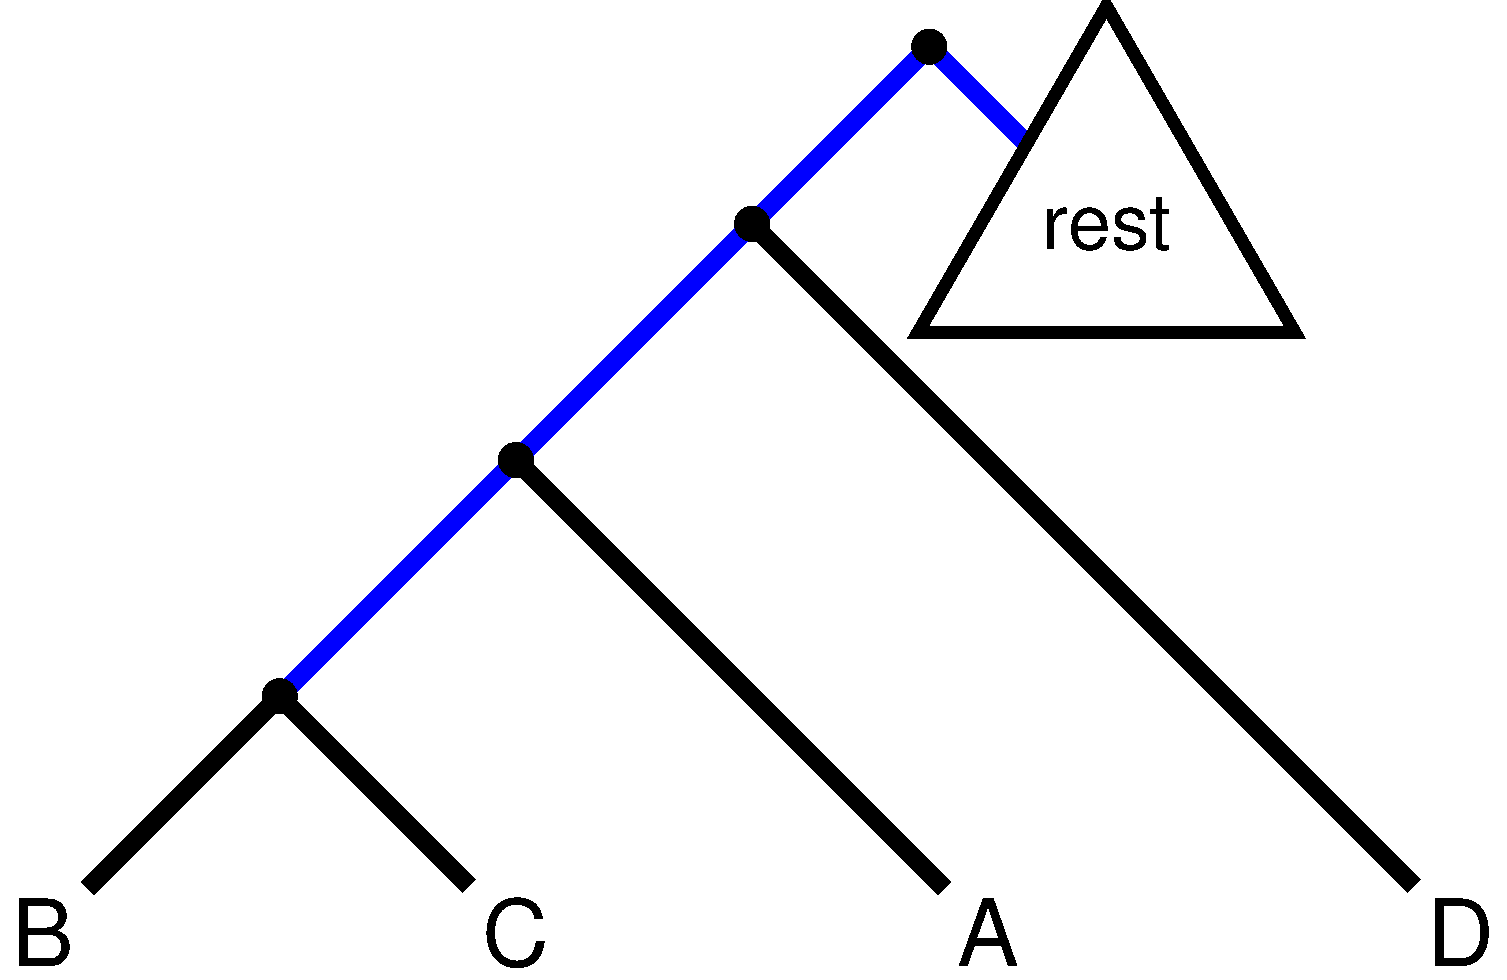
\includegraphics[width=\textwidth]{figures/fastmulrfs-fig2a.pdf}
		~
		\caption{(a) Species tree} 
	\end{subfigure}
	~~~~~~~~~~
	\begin{subfigure}[t]{0.4\textwidth}
	\centering
		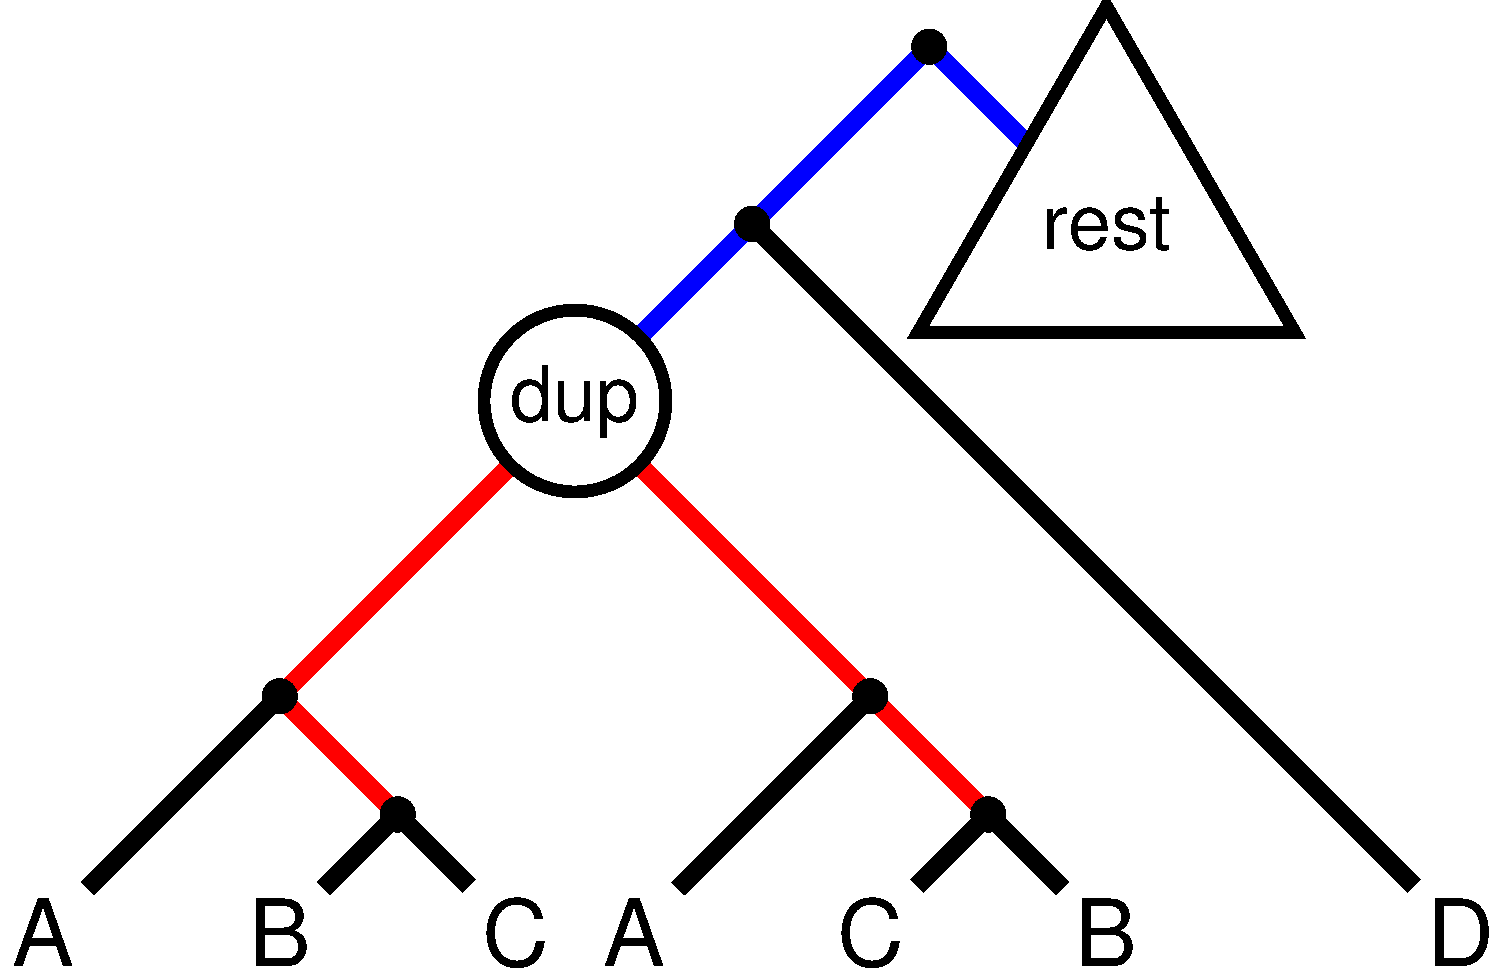
\includegraphics[width=\textwidth]{figures/fastmulrfs-fig2b.pdf}
		~
		\caption{(b) Gene tree: 1 duplication} 
	\end{subfigure}

	\vspace{24pt}

	\begin{subfigure}[t]{0.4\textwidth}
	\centering
		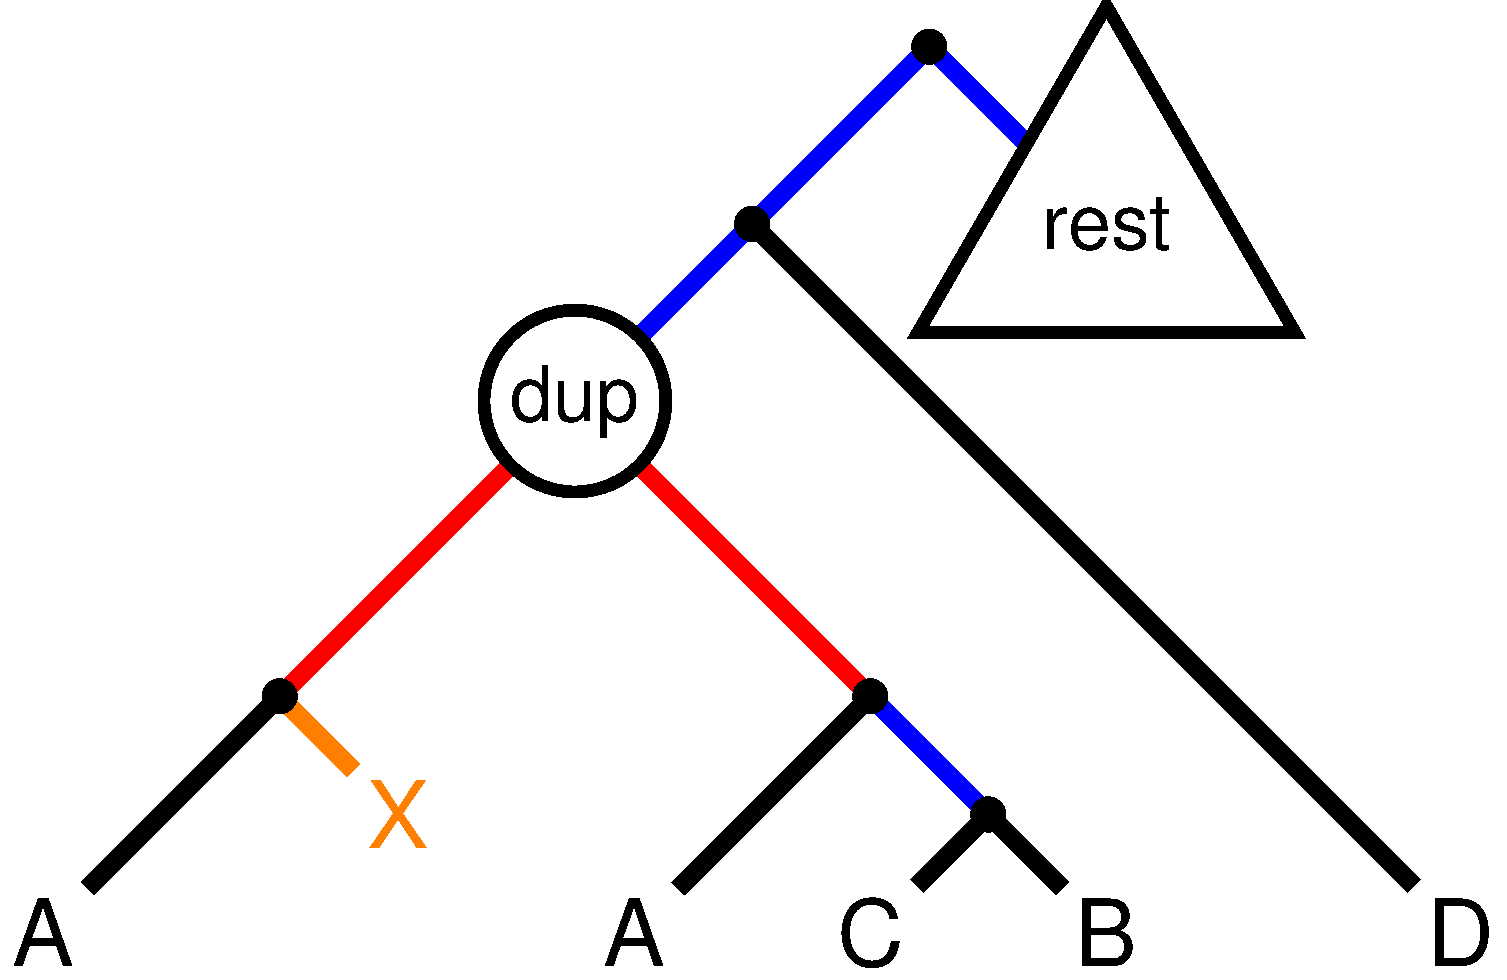
\includegraphics[width=\textwidth]{figures/fastmulrfs-fig2c.pdf}
		~
		\caption{(c) Gene tree: 1 duplication, 1 loss} 
	\end{subfigure}
	~~~~~~~~~~
	\begin{subfigure}[t]{0.4\textwidth}
	\centering
		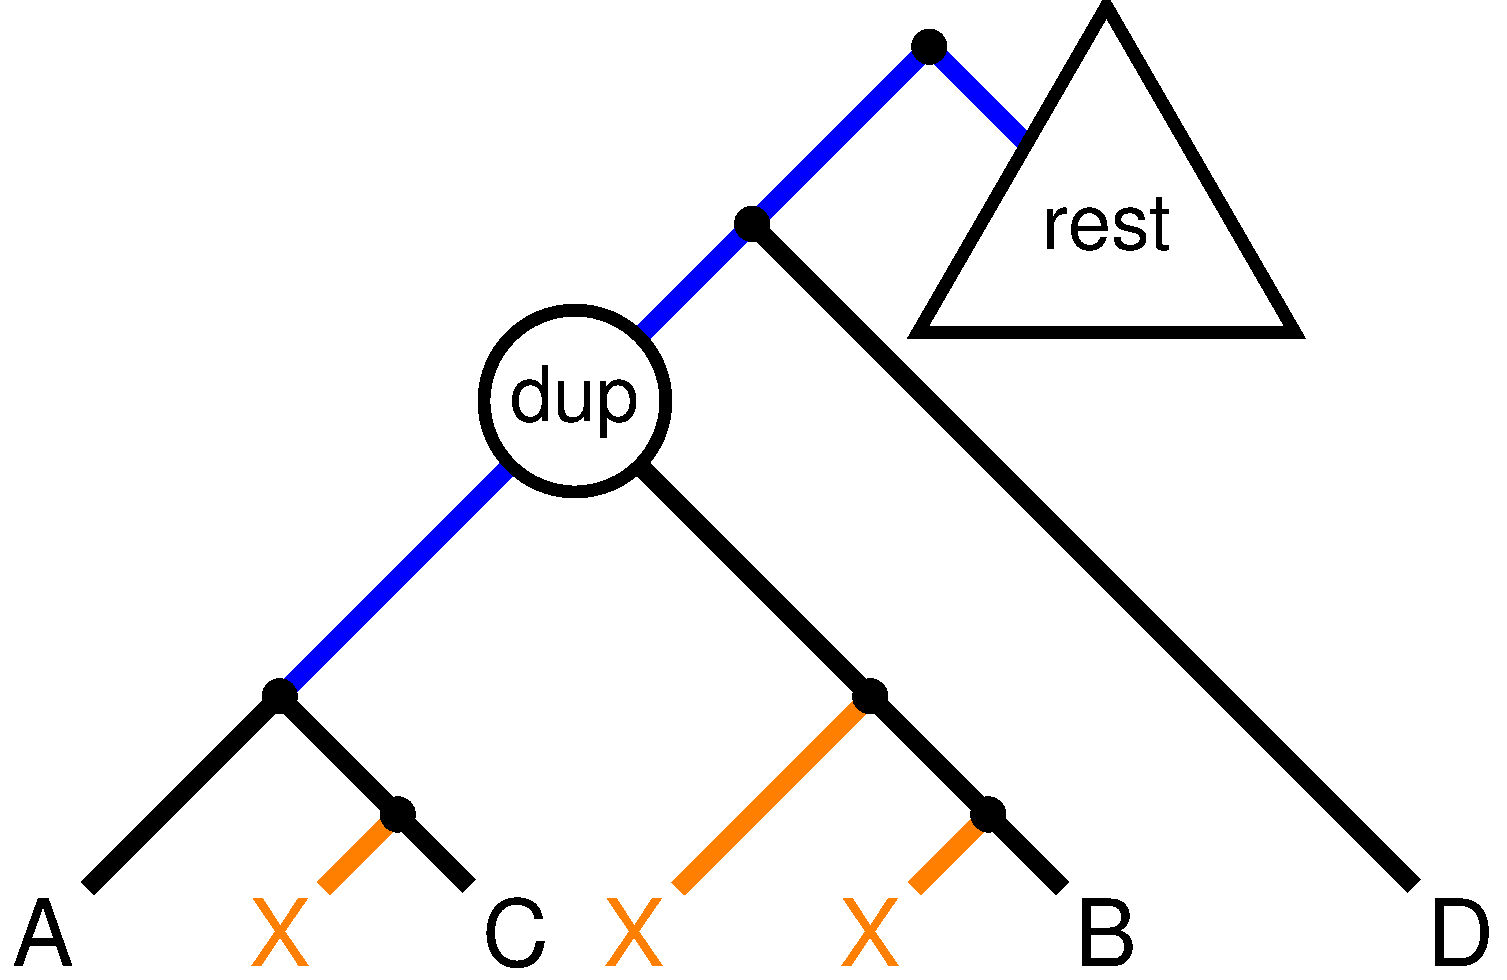
\includegraphics[width=\textwidth]{figures/fastmulrfs-fig2d.pdf}
		~
		\caption{(d) Gene tree: 1 duplication, 3 losses} 
	\end{subfigure}
	\caption{
	{\bf Impact of duplications and losses on RFS-MUL-trees.}
Subfigure (a) shows a rooted species tree and subfigures (b)--(d) show three rooted gene family trees that evolved within the species tree.
Internal edges that induce valid bipartitions are shown in blue, internal edges that induce invalid bipartitions are shown in red, \glspl{terminaledge} are shown in black, and losses are shown in orange.
Subfigure (b) shows a gene family tree with a duplication event on the edge above the MRCA of species $\{ A, B, C \}$, which we refer to as species $Y$. 
All internal edges below the duplication fail to induce bipartitions; therefore, they do not impact the solution space for RFS-MUL-trees.
Subfigure (c) shows a gene family tree with the same duplication event followed by one copy of the gene being lost from the MRCA of species $\{B, C\}$.
Because $A$ retains both copies, the internal edges on the path between $A$ (on the left) and $A$ (on the right) fail to induce bipartitions; therefore, they do not impact the solution space for RFS-MUL-trees.
As long as one species retains both copies of a gene, the two arcs that are incident to the duplication node fail to induce bipartitions, as they must be on the path between two leaves with the same label.
Subfigure (d) shows a gene family tree with the same duplication event followed by one copy of the gene being lost from species $B$ and the other copy of the gene being lost from both species $A$ and $C$.
None of the species that evolved from $Y$ retain both copies of the gene, so all edges below the duplication node induce valid bipartitions.
Because this scenario produces a valid bipartition that is incompatible with the species tree, we refer to this situation as \textit{\gls{adversarialGDL}}. 
	}
	\label{fig:2}
\end{figure}

\clearpage

In the remainder of this section, we will discuss model conditions under which adversarial GDL cannot occur: the {\em duplication-only} case, where all genes evolve with duplication but no loss, and the {\em loss-only} case, where all genes evolve with loss but no duplication.
To prove that a model condition prohibits adversarial GDL, we need to establish that any bipartition that appears in a gene family tree is compatible with the species tree.
Equivalently, any complete bipartition (i.e., a bipartition on the full species set) induced by any gene family tree must also be induced by the species tree, and any incomplete bipartition (i.e., a bipartition on a proper subset of the species set) induced by any gene family tree must be able to be extended (by adding the missing species) so that it becomes a bipartition induced by the species tree (Definition~\ref{def:bipartition-compatibility}).
It is trivial to see that if a gene evolves only with losses, then there is no adversarial GDL for that gene (Lemma \ref{lem:loss}), but the proof for duplication-only evolution is more interesting (Lemma \ref{lem:dup}).

\begin{lemma}
\label{lem:loss}
Let $\mathcal{P}$ be a set of true gene trees that evolved within the rooted species tree $T^*$ under a stochastic loss-only model of gene evolution.
Then, for $\pi \in \{ Bip(M) : M \in \mathcal{P} \}$, $\pi$ is compatible with $T^*$. 
Hence, loss-only models have no adversarial GDL.
\end{lemma}

\begin{lemma}
\label{lem:dup}
Let $\mathcal{P}$ be the set of true gene trees that evolved within the rooted species tree $T^*$ under a stochastic duplication-only model of gene evolution.
Then for every MUL-tree $M \in \mathcal{P}$, $Bip(M) \subseteq Bip(T^*)$.
Hence, duplication-only models have no adversarial GDL.
\end{lemma}

\begin{proof}
Let $M$ be an unrooted version of a MUL-tree in $\mathcal{P}$, and let $e$ be an internal edge in $E(M)$.
We say that an internal edge $e = (x,y) \in E(M)$ lies below a duplication node if there is at least one duplication node on the path from either $x$ or $y$ to the root in the rooted version of $M$; otherwise, we say that $e$ is above all duplication nodes.
An internal edge $e$ is below a duplication node if and only if there is at least one species on both sides of $e$. 
It follows that any internal edge $e$ below a duplication node will be contracted when producing $\mathcal{X}(M)$.
Conversely, an internal edge $e$ is above all duplication nodes if and only if there are no leaves on both sides of $e$ with the same species label.
It follows that any internal edge $e$ above all duplication nodes will {\em not} be contracted when producing $\mathcal{X}(M)$.
Finally, consider a bipartition induced by an edge that is not contracted, and therefore has no duplication nodes above it.
This bipartition appears in the true species tree $T^*$, since the only events that cause the gene family tree to differ from the true species tree are duplications.
\end{proof}

We now prove that FastMulRFS is statistically consistent under generic GDL models if no adversarial GDL occurs.

\begin{theorem}
\label{thm:opt}
The true species tree $T^*$ is an RFS-MUL-trees supertree for any input $\mathcal{P}$ for which no adversarial gene duplication and loss occurred.
\end{theorem}
\begin{proof}
The optimization problem seeks a binary tree $T$ that minimizes the sum of the RF distances to the input MUL-trees; this is equivalent to maximizing the sum of the number of compatible bipartitions in the input MUL-trees. 
If no adversarial GDL occurs, then by definition, every bipartition in the input MUL-trees is compatible with the true species tree $T^*$, and so $T^*$ is an optimal solution to the RFS-MUL-trees problem.
\end{proof}

\begin{theorem}
FastMulRFS is statistically consistent under a generic GDL model for which adversarial GDL is prohibited.
\label{thm:main}

\end{theorem}
\begin{proof}
Let $T^*$ be the true species tree. 
By Theorem \ref{thm:opt}, $T^*$ is an optimal solution to the RFS-MUL-trees problem for any input $\mathcal{P}$ for which no adversarial GDL occurred, so as the number of genes increases, $T^*$ is an optimal solution to the RFS-MUL-trees problem.
FastMulRFS finds an optimal solution to the RFS-MUL-trees problem subject to the output tree $T$ satisfying $Bip(T) \subseteq \Sigma$ (Theorem 3 in \cite{vachaspati2015fastrfs} and Theorem \ref{thm:equal}).
Our generic GDL models assume that the probability of no duplication or loss occurring on an edge is always greater than zero for every gene, so there is a strictly positive probability of the true species tree $T^*$ appearing in the set $\mathcal{P}$ of gene family trees; therefore, as the number of genes increases, $\Sigma$ (as constructed by the default setting within FastMulRFS) will contain all bipartitions in the set $Bip(T^*)$ with probability converging to one.
It follows that, as the number of genes goes to infinity, the probability that FastMulRFS will return $T^*$ converges to one.
\end{proof}

We conclude this section with a conjecture.
\begin{conjecture}
\label{conj:1}
FastMulRFS is statistically consistent under a generic model of GDL for probabilities of gene duplication and loss, so that adversarial GDL has sufficiently low probability.
\end{conjecture}

\section{Performance Study}
\label{sec:fastmulrfs-study}
We evaluated FastMulRFS in comparison to ASTRAL-multi, DupTree, and MulRF on biological and simulated datasets, considering species tree topological accuracy and running time. 

\subsection{Fungal Dataset}
We analyzed a fungal dataset with 16 species and $5\,351$ genes from Rasmussen and Kellis \cite{rasmussen2012unified}, who provided gene family trees estimated from their nucleotide alignments (see Table~\ref{tab:fungi-biological} for an analysis of the number of copies per species in this dataset).
In a prior study, Butler {\em et al.} \cite{butler2009evolution} estimated species trees from this same dataset (specifically the \gls{concatenatedalignment} of putatively orthologous amino acid sequences) using MrBayes \cite{ronquist2003mrbayes}.
The comparison of trees estimated on this biological dataset is difficult to interpret, as the prior concatenation analysis was constrained to enforce the out-grouping of {\em S. castellii} with respect to {\em S. cerevisiae} and {\em C. glabrata}.
Furthermore, the study by Butler {\em et al.} \cite{butler2009evolution} reported several trees that differed with respect to this group (i.e., not all analyses returned this as a clade) as well as with respect to the placement of {\em K. waltii}.
According to their study, none of these resolutions are clearly correct.

\subsection{Simulated Datasets}
\paragraph{Species trees and gene trees:}
We used \gls{SimPhy} version 1.0.2 to simulate a collection of 100-species, 1000-gene datasets under the DLCoal model with six different model conditions: three levels of GDL and two levels of ILS.
The easiest model condition was (largely) based on parameters estimated from the 16-species fungal dataset from Rasmussen and Kellis \cite{rasmussen2012unified} except that we assumed 10 generations per year instead of $1.\bar{1}$ generations per year, which resulted in simulated datasets that were similar to the biological dataset in terms of each species being represented in a similar proportion of gene family trees (Tables~\ref{tab:fungi-biological}--\ref{tab:fungi-simulated}); Supplementary Materials for details.
To make more challenging model conditions, we increased the GDL rate and ILS level by increasing the \gls{EPS}.

We quantified the level of ILS by computing the normalized RF distance between each true \gls{locustree} and its respective true gene tree (which are on the same leaf set), averaging this value across all 1000 locus/gene trees.
The average locus-to-gene tree discord across the 10 replicate datasets was 2\% for the ``no ILS condition'' and 12\% for the ``low/moderate'' ILS condition (note that if we had used 1.1 generations per year, AD would have increased to 19\% and 55\%, respectively).

We also quantified the level of GDL by counting the number of leaves and the number of species per gene tree.
All gene trees had approximately 100 leaves, which is expected since the duplication and loss rates are equal.
As the duplication/loss rate increased, the number of species per gene tree decreased, so even though locus/gene trees had the same number of leaves on average, these leaves were labeled by fewer species.
For duplication/loss rates of $1 \times 10^{-10}$, $2 \times 10^{-10}$, and  $5 \times 10^{-10}$ the average number of species per gene tree was 85, 74, and 53.

We allowed gene trees to deviate from a \gls{strictmolecularclock} by using gene-by-lineage-specific rate heterogeneity modifiers, meaning that for each gene tree, a gamma distribution was defined for each gene tree by drawing $\alpha$ from a log-normal distribution with a location of 1.5 and a scale of one (same parameters as used in \cite{zhang2018astral}), and then each branch length in a gene tree was multiplied by a value drawn the gamma distribution corresponding to that gene tree.

\paragraph{DNA (gene) sequence data:}
We now describe the simulation of DNA sequence data for each gene tree produced by SimPhy.
Again, our protocol is also based on the fungal dataset from Rasmussen and Kellis \cite{rasmussen2012unified}, who provided an estimated \gls{MSA} and an estimated \gls{ML} tree for each of the $5\,351$ genes.
We estimated \gls{GTR+GAMMA} model parameters ($\vec{\pi}$, $Q$, and $\alpha$) for each MSA and ML gene tree pair using \gls{RAxML} version 8.2.12 and then fit distributions to the estimated GTR+GAMMA model parameters (only MSAs with least 500 \gls{parsimony-informative} sites and at most 25\% \glspl{gap} were included in this analysis).
For each gene tree, we drew GTR+GAMMA model parameters from these distributions and then simulated DNA sequences (with 1000 sites) using \gls{INDELible} version 1.03.
Because DNA sequences were simulated without insertions or deletions, MSA estimation was not necessary.

\paragraph{Estimated gene trees:}
ML gene trees were estimated under the GTR+GAMMA model using RAxML version 8.2.12. 
Prior to gene tree estimation, sequences were truncated to the first 25, 50, 100, and 250 nucleotides to produce datasets with varying levels of GTEE.
GTEE was measured by the normalized RF distance between the true and the estimated gene family trees.
Sequence lengths of 25, 50, 100, and 250 resulted in mean GTEE of 67\%, 52\%, 35\%, and 19\%, respectively.

\subsection{Species Tree Estimation}
Finally, species trees were estimated on 25, 50, 100, and 500 gene family trees, either true or estimated, using three different methods: ASTRAL-multi (as implemented in ASTRAL version 5.6.3), DupTree, FastMulRFS (as implemented in release 1.2.0 version 3), and MulRF (as implemented in version 2.1).
All estimated species trees were binary (note that a single optimal tree was taken as an estimate of the species tree even when multiple equally optimal trees were returned by FastMulRFS).
This created $120$ model conditions (three GDL rates, two levels of ILS, five levels of GTEE, and four numbers of genes), each with 10 replicates, for a total of $1\,200$ datasets.

\subsection{Evaluation}
Species tree estimation methods were evaluated in terms of running time and species tree error, as measured by the \gls{RFerrorrate} (Equation~\ref{eq:rf-error}).
All computational experiments were performed on the Campus Cluster at the University of Illinois at Urbana-Champaign, which is a heterogeneous system, meaning that compute nodes can have different specifications (\href{https://campuscluster.illinois.edu/resources/docs/nodes/}{https://campuscluster.illinois.edu/resources/docs/nodes/}).

\section{Results}
\label{sec:fastmulrfs-results}
\subsection{Fungal Dataset}
In an analysis of the fungal dataset, all methods (ASTRAL-multi, FastMulRFS, DupTree, and MulRF) produced species trees that were similar to the MrBayes concatenation tree (Figure \ref{fig:fungi}).
The differences in species trees are minor given the variability in the trees found by Butler {\em et al.} \cite{butler2009evolution}, the use of a topological constraint in their MrBayes analysis, and the uncertainty about the placement of specific taxa in the tree (see Supplementary Information Section 5 in \cite{butler2009evolution} for more information).  

Given that the topological differences are minor and difficult to interpret, we focus on differences in empirical running time.
FastMulRFS and DupTree completed in under a minute each, ASTRAL-multi completed in 18 minutes, and MulRF completed in 40 minutes.
Hence, FastMulRFS is much faster than MulRF and ASTRAL-multi.
While all four of these methods were relatively fast on 16 taxa, we expect the difference between methods to increase on datasets with larger numbers of species and with higher rates of gene duplication.
The improvement in running time over MulRF and ASTRAL-multi is due in part to the fact that both MulRF and ASTRAL-multi use the original gene family trees, while FastMulRFS uses the reduced singly-labeled trees; hence, as the number of leaves or the duplication rate increase, the advantage in running time for FastMulRFS should also increase.

\begin{figure}[!h]
	\centering
	%\includegraphics[width=1.0\textwidth]{figures/fastmulrfs-fig3.pdf}
	\begin{subfigure}[t]{0.31\textwidth}
	\centering
		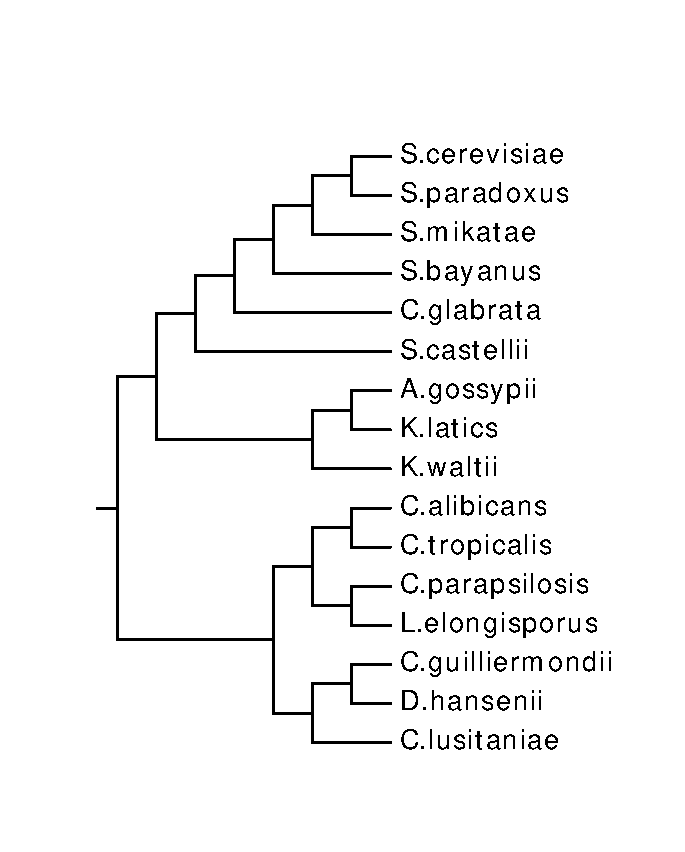
\includegraphics[width=\textwidth]{figures/fastmulrfs-fig3a.pdf}
		\caption{(a) Concatenation} 
	\end{subfigure}
	~
	\begin{subfigure}[t]{0.31\textwidth}
	\centering
		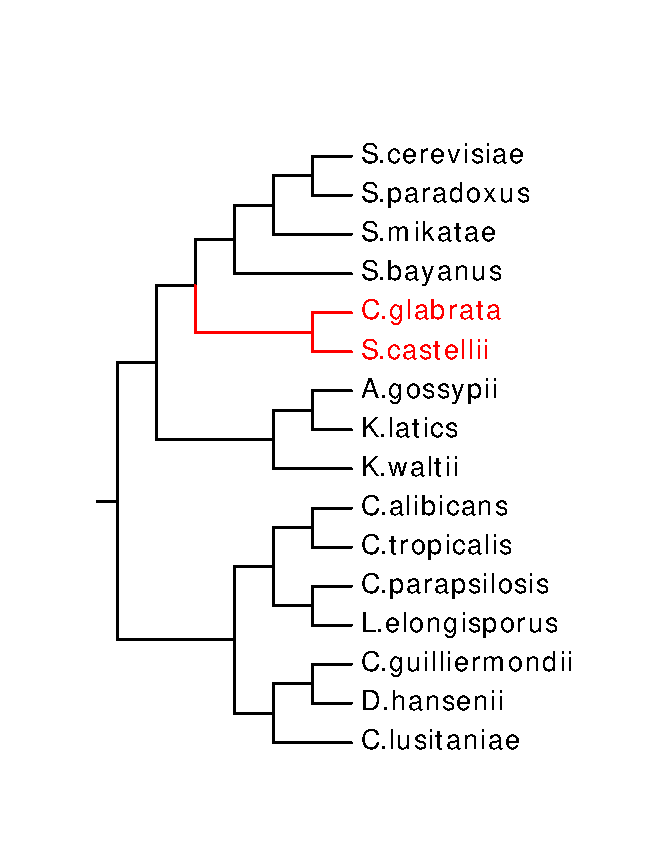
\includegraphics[width=\textwidth]{figures/fastmulrfs-fig3b.pdf}
		\caption{(b) ASTRAL-multi} 
	\end{subfigure}
	~
	\begin{subfigure}[t]{0.31\textwidth}
	\centering
		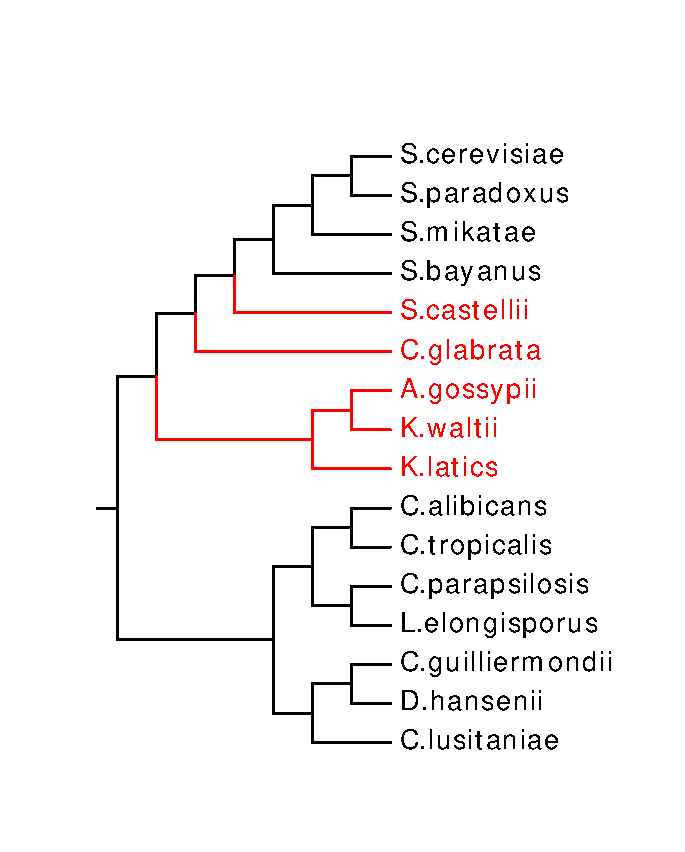
\includegraphics[width=\textwidth]{figures/fastmulrfs-fig3c.pdf}
		\caption{(c) FastMulRFS} 
	\end{subfigure}
   \caption{Species trees were estimated on the 16-taxon fungal dataset with $5\,351$ gene family trees estimated by Rasmussen and Kellis \cite{rasmussen2012unified}. 
   Subfigure (a) shows the MrBayes concatenation tree estimated by Butler {\em et al.} \cite{butler2009evolution}, which is based on putative orthologs instead of the gene family trees.
   Subfigure (b) shows the ASTRAL-multi tree, and subfigure (c) shows the FastMulRFS tree, which is the same tree produced by MulRF and DupTree.
   Topological differences between the MrBayes concatenation tree are highlighted in red; however, this is not indicative of which resolution is correct or incorrect, as the true placement of these taxa is not yet established.
   DupTree and FastMulRFS were the fastest (both completed in less than a minute), ASTRAL-multi estimated a species tree in 18 minutes, and MulRF completed in 40 minutes.}
   \label{fig:fungi}
\end{figure}

\subsection{Simulated Datasets}
DupTree typically had poorer accuracy than the other tested methods (Figures~\ref{fig:fastmulrfs-500gen}--ref{fig:fastmulrfs-100gen}), especially when the level of GTEE was high.
As high GTEE is consistent with the generally low bootstrap branch support values reported for several multi-locus datasets (Table \ref{tab:include-1}), we focus on comparing MulRF, FastMulRFS, and ASTRAL-multi.
All methods improved in accuracy with larger numbers of genes and degraded in accuracy with higher GTEE levels, ILS levels, and/or GDL rates.
The relative accuracy between methods was consistent across all model conditions, although the degree of difference depended on the model conditions, with bigger differences for smaller numbers of genes and higher GTEE levels, ILS levels, and GDL rates.
When given 500 gene trees, error levels were low and differences between methods were (usually) small, so that the main difference was running time.
The fastest method was FastMulRFS, MulRF was the slowest, and ASTRAL-multi was intermediate.

\paragraph{FastMulRFS vs.~MulRF:}
FastMulRFS and MulRF are both heuristics for the RFS-MUL-trees problem.
They were essentially tied for accuracy across all tested conditions (Figures~\ref{fig:fastmulrfs-500gen}--\ref{fig:fastmulrfs-100gen} and Table \ref{tab:fastmulrfs-error}), but FastMulRFS was dramatically faster than MulRF (Figures~\ref{fig:fastmulrfs-500gen}--\ref{fig:fastmulrfs-100gen} and Table \ref{tab:fastmulrfs-rt}). In addition, FastMulRFS nearly always returned a tree with an equivalent or better RFS-MUL-trees score than MulRF. Out of the $1\,200$ datasets analyzed, FastMulRFS was worse than MulRF on 56 datasets, FastMulRFS was equal to MulRF on  962 datasets, and FastMulRFS was better than MulRF on 182 datasets.

\paragraph{FastMulRFS vs.~ASTRAL-multi:}
FastMulRFSwas always at least as accurate on average as ASTRAL-multi (and was often more accurate on average  than ASTRAL-multi) across all model conditions tested (Figures~\ref{fig:fastmulrfs-500gen}--\ref{fig:fastmulrfs-100gen} and Table \ref{tab:fastmulrfs-error}), with larger differences between methods for the higher GTEE conditions and smaller differences for the lower GTEE conditions.
The running times for ASTRAL-multi and FastMulRFS increased with the number of genes, but FastMulRFS was always faster (Figures~\ref{fig:fastmulrfs-500gen}--\ref{fig:fastmulrfs-100gen} and Table \ref{tab:fastmulrfs-rt}).
For example, on the 500-gene model conditions, FastMulRFS typically completed in one to two minutes (and always in under five minutes), whereas ASTRAL-multi used between 10 minutes and 1.2 hours.

\section{Discussion}
To date, only two types of methods have been proven statistically consistent under any GDL model.
The first type of method is based on maximizing quartets that are induced by the gene family trees, and the second type of method  is based on maximizing bipartitions that are induced by the gene family trees.
ASTRAL-multi is an example of the first kind of method, and FastMulRFS is an example of the second type of method; notably, both methods use DP to solve their optimization problems exactly within a constrained search space.
The conditions under which these two methods have been proven statistically consistent are different. 
ASTRAL-multi is established to be consistent under a gene evolution model that requires that all the genes evolve {\em i.i.d.}~within the species tree.
Since the time of our study, Markin and Eulenstein \cite{markin2020quartet} showed that a related quartet-based approach is statistically consistent under the DLCoal model, which allows for both GDL and ILS but still assumes that genes evolve {\em i.i.d.}~within the species tree.
In contrast, FastMulRFS has been proven consistent under a generic model that does not require the genes to evolve {\em i.i.d.}~and indeed allows for a very generic model similar to the NCM model.
This is a relative strength of FastMulRFS, as genes do not evolve {\em i.i.d.}~within a species tree, as discussed in \cite{dondi2019reconciling}.
On the other hand, FastMulRFS has only been proven consistent when no adversarial GDL occurs and no ILS occurs; this is a relative weakness of FastMulRFS (although see Conjecture \ref{conj:1} regarding adversarial GDL).
Therefore, from a theoretical perspective, there are advantages and disadvantages for both methods.

In terms of empirical performance, FastMulRFS was more accurate and more robust to GTEE than ASTRAL-multi under most model conditions we examined.
The only conditions in which the two methods achieved similar accuracy were characterized by low GTEE and large numbers of genes, where both methods achieved very high accuracy.
FastMulRFS also was much faster than ASTRAL-multi, with large improvements in speed for large numbers of genes and high GTEE.
In summary, FastMulRFS had superior performance compared to ASTRAL-multi in our experimental evaluation.

A comparison between FastMulRFS and MulRF is also interesting.
Both methods attempt to solve the same NP-hard optimization problem, and neither is guaranteed to find an optimal solution. 
However, FastMulRFS is guaranteed to find an optimal solution within a constrained search space in polynomial time; furthermore, the way that FastMulRFS constrains its search space is sufficient to ensure that it is statistically consistent.
MulRF, in contrast, uses a locally optimal search strategy combined with hill climbing, so it does not run in polynomial time and may not be provably statistically consistent.
In our experimental study, the two methods were very close in accuracy, but FastMulRFS was dramatically faster. 
Overall, FastMulRFS was superior to MulRF.

FastMulRFS matched or improved on the other methods under all conditions we explored, where gene trees evolved under a unified model of ILS and GDL (which did not prohibit adversarial GDL).
Our study suggests that FastMulRFS may have good robustness and high accuracy, even under conditions where it has not (yet) been proven statistically consistent. 
(note that we think it is unlikely that FastMulRFS is statistically consistent under conditions with high ILS.)
Future work is clearly needed to evaluate FastMulRFS and other methods under a wider range of model conditions, including explicit conditions where adversarial GDL and high levels of ILS occur.
Simulations should also be performed to evaluate other scenarios that produce multi-copy genes, for example whole genome duplication events, which impact species tree estimation for many major clades, including fungi \cite{butler2009evolution} and plants \cite{leebensmack2019one}.
More complex simulations also should be performed (including gene conversion and HGT) in order to better understand the conditions in which methods perform well. 
Along these lines, it would be helpful to characterize biological datasets to understand realistic levels of ILS and GDL (including the frequency of adversarial GDL); this task has been identified as an important challenge throughout this dissertation. 

A limitation of this study is that we examined only a few methods, and future studies should evaluate other methods, including {\em guenomu} (discussed earlier) and MixTreEM \cite{ullah2015species-mixtrem}, to discover the places in the parameter space of model species trees where each method outperforms the others.
Furthermore, methods that operate by making predictions of orthology could be used in a three-phase approach: given inputs with sequence alignments and MUL-trees, predict orthology, reduce to datasets with just orthologous genes (and hence singly-labeled gene trees), and then run a preferred species tree estimation method. 
For example, in a recent preprint, Zhang {\em et al.} \cite{zhang2020astral-pro} presented A-PRO, another modification of ASTRAL, and proved that it is statistically consistent under a GDL model if given correctly ``tagged" gene trees (i.e., each node in each gene tree is correctly identified as either a duplication or not); however, this assumption means that orthology can be inferred without error (an assumption that is not made for ASTRAL-multi).
Studies evaluating A-PRO and these other approaches under a variety of conditions would enable biologists to select methods with the best expected accuracy for their datasets.

While we have focused on the estimated species topology, biologists require that branches in the topology to be annotated with information about the support for or confidence in each branch.
Our reduction on MUL-trees (which transforms them into singly-labeled trees) is useful not only for estimating species trees but also for interpreting estimated species trees.

First, the reduction allows the branches of the species tree to be annotated by the proportion of MUL-trees that contain that branch; this metric is easy to interpret and therefore highly useful.
Second, by combining the reduction with DP in a constrained search space, we can use an existing tool, called SIESTA \cite{vachaspati2017enhancing}, to quantify the space of optimal solutions; specifically, SIESTA reports the number of optimal solutions in the constrained search space and annotates each branch by the proportion of optimal solutions that contain that branch.
This seems especially useful in the context of duplication and loss, as the reduction on MUL-trees illustrates that the MUL-trees are likely to be unresolved when duplications occur; this combined with losses could result in a large space of optimal solutions.

Third, after applying the reduction to MUL-trees, it possible to determine the relative weight of each MUL-tree when solving the RFS-MUL-trees problem.
A MUL-tree $M$ that evolves with only a duplication at a leaf induces $S(M) - 3$ valid bipartitions; however, a MUL-tree that evolves with only a duplication at the root induces zero valid bipartitions; therefore, the output tree could be biased towards a small subset of MUL-trees that contain a disproportionately large number of valid bipartitions compared to the other MUL-trees in the input set.
While this is not a problem in theory, it can be a problem in practice, as MUL-trees can differ from the species tree due to estimation error and other sources of heterogeneity.
This has already been shown to be an issue in the context of ILS.
As an example, gene trees with different numbers of species induce different numbers of quartets, and in this case, each gene tree contributes a different number of quartets to the MQSS problem (which ASTRAL solves within a constrained search space).
Two recent studies \cite{gatesy2017resolving-pcs, gatesy2019partitioned} showed that the resolution of some controversial branches can change by removing outlier gene trees that contribute a disproportionately large number of quartets compared to the other gene trees in the input set.
The ability to recognize that two fully resolved MUL-trees can contribute very different numbers of bipartitions to the RFS-MUL-trees problem is critical for identifying systematic biases, and we hope the theoretical observations of our study further enable the interpretation of species trees estimated from gene family trees.

\section{Conclusions}
\label{sec:conclusions}
We presented FastMulRFS, a new method for estimating species tree from unrooted gene family trees, without needing to have any information about orthology.
FastMulRFS runs in polynomial-time and is provably statistically consistent under a generic GDL when adversarial GDL does not occur.
Prior to our study, the only method established to be statistically consistent under any GDL model was ASTRAL-multi (their proof does assume that genes evolve {\em i.i.d.}~within the species tree but does not prohibit adversarial GDL).
Of course, statistical consistency does not predict performance on finite amounts of data or in the context of model violations (which are perhaps certain to occur when analyzing biological datasets).
In our simulation study, FastMulRFS compared quite favorably (in terms of accuracy and running time) to ASTRAL-multi as well as MulRF.
This is significant as we evaluated methods under conditions where neither FastMulRFS nor ASTRAL-multi are (yet) proven to be statistically consistent. 
Specifically, our proof establishes statistical consistency (of FastMulRFS) under models where ILS, GTEE, or adversarial GDL are prohibited, whereas our study benchmarks methods on datasets simulated with two ILS levels, five GTEE levels, and three GDL rates (note that adversarial GDL was not explicitly prohibited).
Although accuracy is difficult to evaluate on biological datasets, FastMulRFS produced trees that were similar to those produced by other methods and did not violate known relationships.
Overall, the recent advances in development of statistically consistent methods for species tree estimation under GDL models is exciting, and the good performance of many of these methods under a range of model conditions suggests that novel combinations and ideas may lead to even better methods that provide improved accuracy and scalability.

\clearpage

\section{Plots}
\label{sec:fastmulrfs-plots}
This section contains the four plots presented in Section~\ref{sec:fastmulrfs-results} Results. 

\vspace{12pt}

\begin{figure}[!h]
\centering
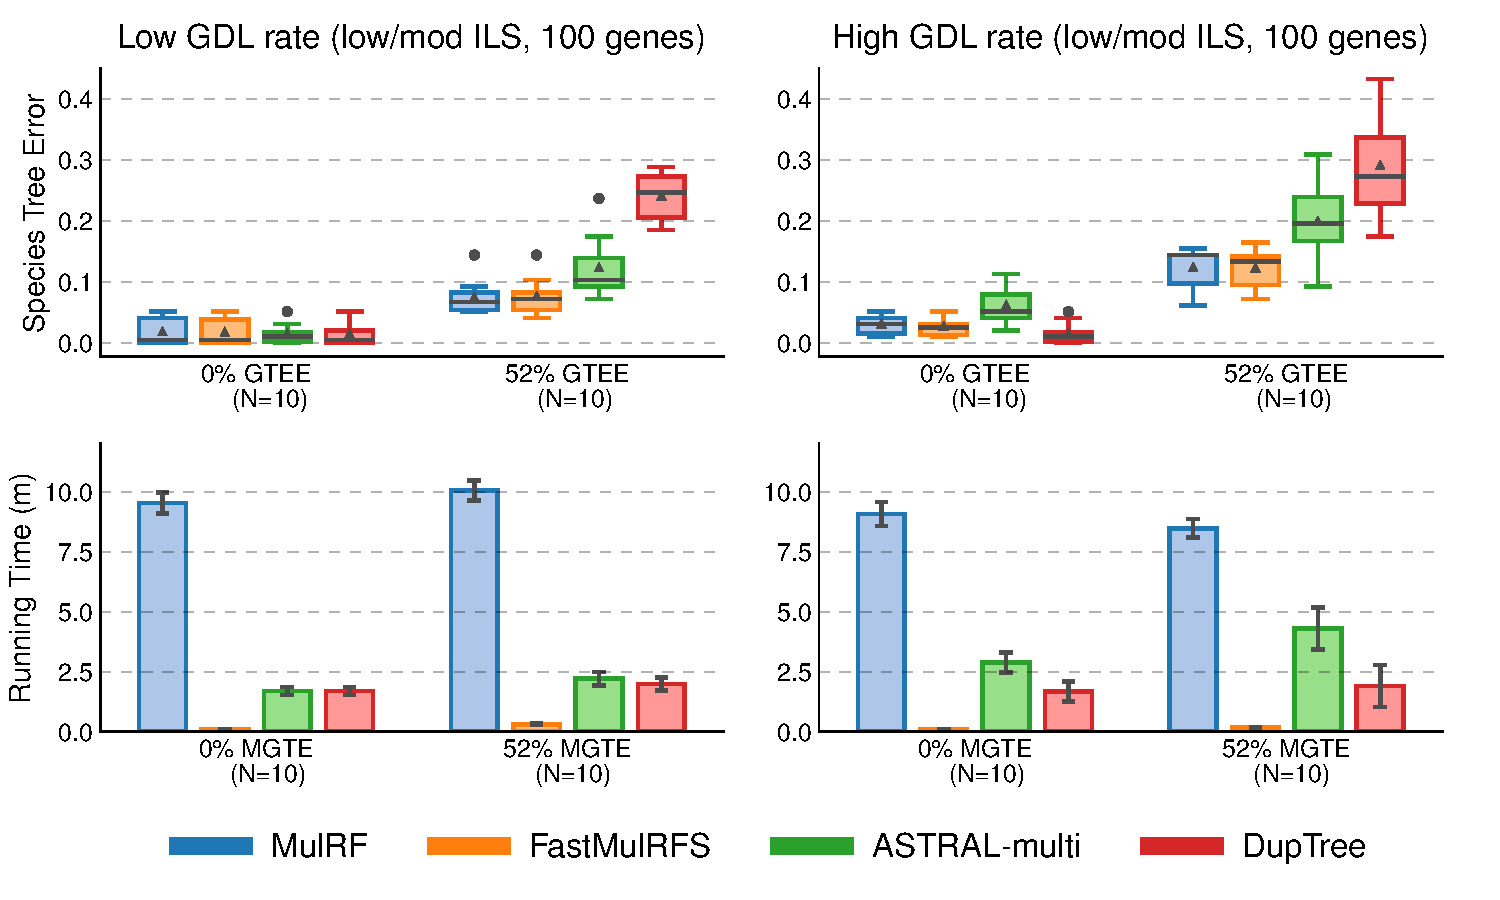
\includegraphics[width=\textwidth]{figures/fastmulrfs-fig4.pdf}
	\caption{{\bf Comparison of species tree estimation methods on 500 gene datasets with low/moderate ILS.} 
	MulRF (blue), FastMulRFS (orange), ASTRAL-multi (green), and DupTree (red) are compared on 100-species, 500 gene datasets with low/moderate ILS (12\%), two levels of GTEE, and two GDL rates (lowest and highest).
	Subplots in the top row show species tree error (RF error rate).
Gray bars represent medians, gray triangles represent means, gray circles represent outliers, box plots are defined by quartiles (extending from the first to the third quartiles), and whiskers extend to plus/minus 1.5 times the interquartile distance (unless greater/less than the maximum/minimum value).
Subplots in the bottom row show running time (in minutes); bars represent means and error bars represent standard deviations across replicate datasets.).
The number $N$ of replicates on which the methods completed is shown on the $x$-axis.}
\label{fig:fastmulrfs-500gen}
\end{figure}

\begin{figure}[!h]
	\centering
	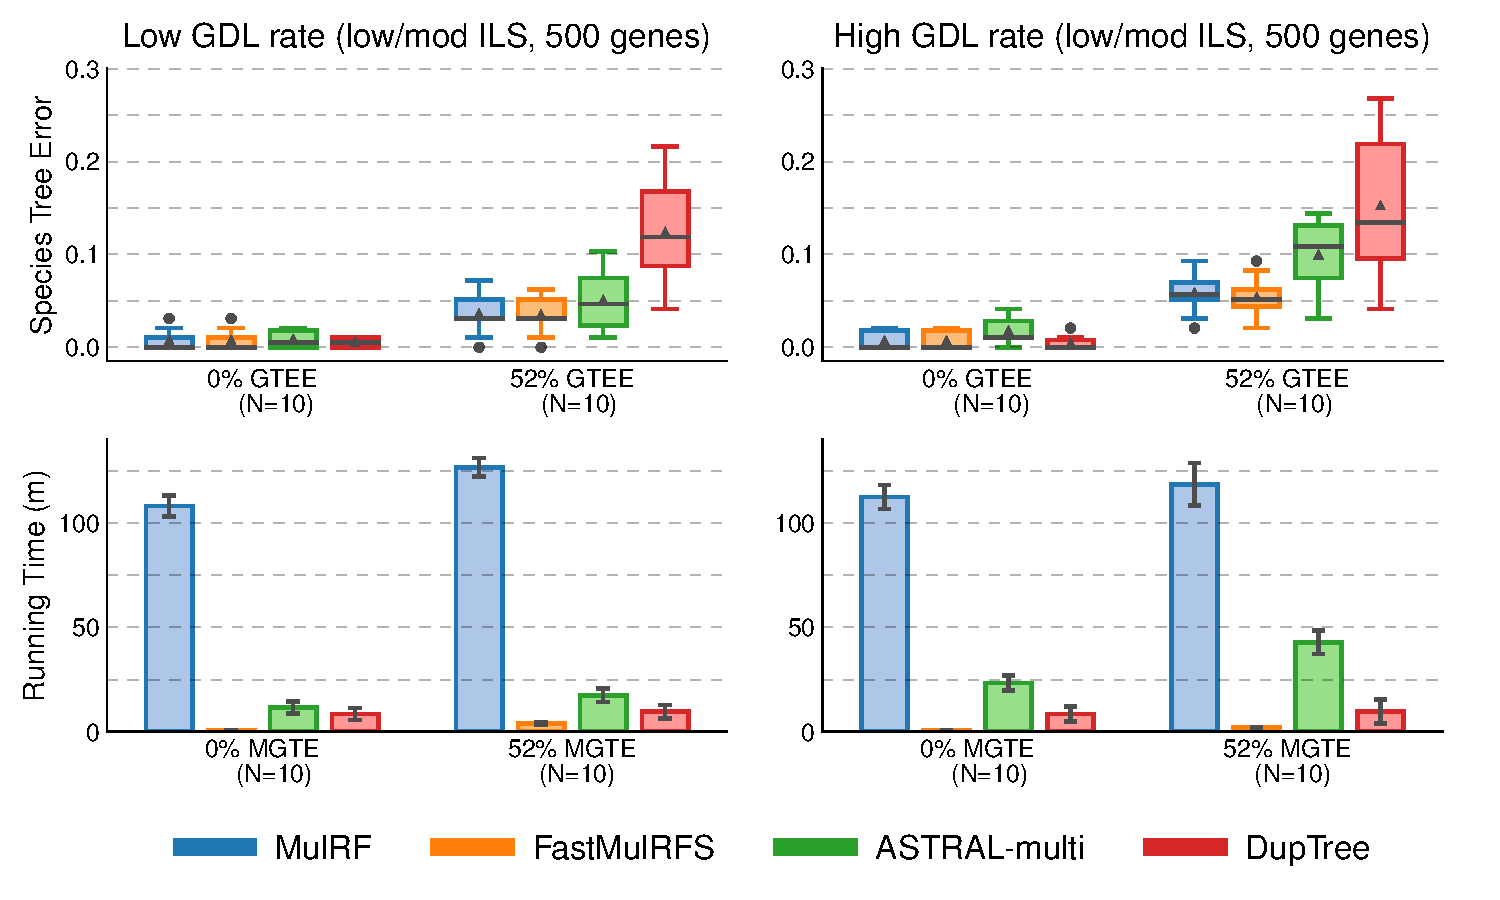
\includegraphics[width=\textwidth]{figures/fastmulrfs-fig5.pdf}
	\caption{{\bf Comparison of species tree estimation methods on 100 gene datasets with low/moderate ILS.} 
	MulRF (blue), FastMulRFS (orange), ASTRAL-multi (green), and DupTree (red) are compared on 100-species, 100 gene datasets with low/moderate ILS (12\%), two levels of GTEE, and two GDL rates (lowest and highest).
	Subplots in the top row show species tree error (RF error rate).
Gray bars represent medians, gray triangles represent means, gray circles represent outliers, box plots are defined by quartiles (extending from the first to the third quartiles), and whiskers extend to plus/minus 1.5 times the interquartile distance (unless greater/less than the maximum/minimum value).
Subplots in the bottom row show running time (in minutes); bars represent means and error bars represent standard deviations across replicate datasets.).
The number $N$ of replicates on which the methods completed is shown on the $x$-axis.}
\label{fig:fastmulrfs-100gen}	
\end{figure}

\clearpage

\section{Tables}
\label{sec:fastmulrfs-tables}
This section contains the two tables presented in Section~\ref{sec:fastmulrfs-study} Performance Study and the two tables presented in \ref{sec:fastmulrfs-results} Results. 

\vspace{12pt}

\begin{table}[!h]
\centering
\setlength{\tabcolsep}{6pt}
%\footnotesize
\caption{{\bf Statistics on the number of copies of each species in the fungal datasets.} 
For the fungal biological dataset, we computed the mean ($\pm$ standard deviation), the minimum, and the maximum number of copies of each species across $5\,351$ gene trees.
We also report the proportion of gene family trees with more than 1, 2, 5, 10, and 20 copies of a species; for example, $>1$ indicates the proportion of gene family trees (out of $5\,351$) with greater than one copy of the species.
}\label{tab:fungi-biological}
\begin{tabular}{ccccc ccccc}
\toprule
Species & Mean $\pm$ Std & Min & Max & $=$1 & $>$1 & $>$2 & $>$5 & $>$10 & $>$20\\
\midrule
 A. gossypii & 0.85 $\pm$ 0.58 & 0 & 13 & 0.731 & 0.050 & 0.008 & 0.001 & 0.000 & 0.000\\
 C. alibicans & 1.04 $\pm$ 0.65 & 0 & 7 & 0.769 & 0.111 & 0.027 & 0.001 & 0.000 & 0.000\\
 C. glabrata & 0.93 $\pm$ 0.81 & 0 & 27 & 0.667 & 0.110 & 0.019 & 0.002 & 0.001 & 0.000\\
 C. guilliermondii & 0.99 $\pm$ 0.70 & 0 & 11 & 0.722 & 0.110 & 0.027 & 0.001 & 0.000 & 0.000\\
 C. lusitaniae & 0.95 $\pm$ 0.62 & 0 & 10 & 0.728 & 0.098 & 0.019 & 0.000 & 0.000 & 0.000\\
 C. parapsilosis & 1.00 $\pm$ 0.73 & 0 & 12 & 0.729 & 0.110 & 0.028 & 0.003 & 0.000 & 0.000\\
 C. tropicalis & 1.04 $\pm$ 0.73 & 0 & 8 & 0.738 & 0.122 & 0.033 & 0.003 & 0.000 & 0.000\\
 D. hansenii & 1.02 $\pm$ 0.65 & 0 & 7 & 0.756 & 0.110 & 0.026 & 0.002 & 0.000 & 0.000\\
 K. latics & 0.89 $\pm$ 0.63 & 0 & 15 & 0.745 & 0.063 & 0.010 & 0.002 & 0.000 & 0.000\\
 K. waltii & 0.88 $\pm$ 0.71 & 0 & 18 & 0.736 & 0.059 & 0.011 & 0.002 & 0.001 & 0.000\\
 L. elongisporus & 0.98 $\pm$ 0.66 & 0 & 9 & 0.727 & 0.108 & 0.021 & 0.001 & 0.000 & 0.000\\
 S. bayanus & 0.94 $\pm$ 0.81 & 0 & 23 & 0.643 & 0.128 & 0.022 & 0.002 & 0.000 & 0.000\\
 S. castellii & 1.01 $\pm$ 0.91 & 0 & 25 & 0.638 & 0.154 & 0.028 & 0.003 & 0.001 & 0.000\\
 S. cerevisiae & 1.03 $\pm$ 1.09 & 0 & 42 & 0.678 & 0.141 & 0.027 & 0.004 & 0.001 & 0.001\\
 S. mikatae & 0.92 $\pm$ 0.76 & 0 & 18 & 0.646 & 0.118 & 0.021 & 0.002 & 0.000 & 0.000\\
 S. paradoxus & 0.95 $\pm$ 0.83 & 0 & 25 & 0.649 & 0.129 & 0.023 & 0.002 & 0.000 & 0.000\\
\bottomrule
\end{tabular}
\end{table}

\clearpage

\begin{table}[!h]
\centering
\setlength{\tabcolsep}{4pt}
%\footnotesize
\caption{{\bf Statistics on the number of copies of each species in the datasets simulated based on the fungal dataset.} This is the same as Table~\ref{tab:fungi-biological} but data for the first 15 species in the first replicate datasets are shown.}
\label{tab:fungi-simulated}
\begin{tabular}{ccccc ccccc}
\toprule
Species & Mean $\pm$ Std & Min & Max & $=$1 & $>$1 & $>$2 & $>$5 & $>$10 & $>$20\\
\midrule
\multicolumn{10}{l}{\em Assuming 10 generations per year}\\[0.5ex]
 1 & 1.02 $\pm$ 0.57 & 0 & 4 & 0.743 & 0.128 & 0.021 & 0.000 & 0.000 & 0.000\\
 2 & 1.01 $\pm$ 0.60 & 0 & 4 & 0.703 & 0.144 & 0.018 & 0.000 & 0.000 & 0.000\\
 3 & 0.99 $\pm$ 0.56 & 0 & 5 & 0.736 & 0.119 & 0.012 & 0.000 & 0.000 & 0.000\\
 4 & 1.01 $\pm$ 0.60 & 0 & 4 & 0.703 & 0.142 & 0.019 & 0.000 & 0.000 & 0.000\\
 5 & 1.01 $\pm$ 0.61 & 0 & 4 & 0.707 & 0.140 & 0.024 & 0.000 & 0.000 & 0.000\\
 6 & 1.02 $\pm$ 0.57 & 0 & 4 & 0.748 & 0.124 & 0.021 & 0.000 & 0.000 & 0.000\\
 7 & 1.05 $\pm$ 0.57 & 0 & 3 & 0.726 & 0.151 & 0.019 & 0.000 & 0.000 & 0.000\\
 8 & 1.02 $\pm$ 0.58 & 0 & 4 & 0.747 & 0.125 & 0.020 & 0.000 & 0.000 & 0.000\\
 9 & 1.01 $\pm$ 0.57 & 0 & 4 & 0.738 & 0.126 & 0.019 & 0.000 & 0.000 & 0.000\\
 10 & 1.02 $\pm$ 0.56 & 0 & 4 & 0.759 & 0.121 & 0.019 & 0.000 & 0.000 & 0.000\\
 11 & 1.02 $\pm$ 0.58 & 0 & 4 & 0.742 & 0.127 & 0.023 & 0.000 & 0.000 & 0.000\\
 12 & 0.99 $\pm$ 0.56 & 0 & 5 & 0.743 & 0.114 & 0.013 & 0.000 & 0.000 & 0.000\\
 13 & 0.96 $\pm$ 0.59 & 0 & 4 & 0.709 & 0.119 & 0.016 & 0.000 & 0.000 & 0.000\\
 14 & 1.01 $\pm$ 0.60 & 0 & 4 & 0.732 & 0.124 & 0.025 & 0.000 & 0.000 & 0.000\\
 15 & 1.01 $\pm$ 0.63 & 0 & 4 & 0.693 & 0.145 & 0.022 & 0.000 & 0.000 & 0.000\\[2ex]
 \multicolumn{10}{l}{\em Assuming $1.\bar{1}$ generations per year}\\[0.5ex]
 1 & 0.99 $\pm$ 0.20 & 0 & 3 & 0.961 & 0.015 & 0.001 & 0.000 & 0.000 & 0.000\\
 2 & 0.99 $\pm$ 0.21 & 0 & 2 & 0.955 & 0.017 & 0.000 & 0.000 & 0.000 & 0.000\\
 3 & 0.99 $\pm$ 0.18 & 0 & 2 & 0.968 & 0.012 & 0.000 & 0.000 & 0.000 & 0.000\\
 4 & 1.00 $\pm$ 0.22 & 0 & 3 & 0.954 & 0.021 & 0.001 & 0.000 & 0.000 & 0.000\\
 5 & 1.00 $\pm$ 0.22 & 0 & 2 & 0.950 & 0.024 & 0.000 & 0.000 & 0.000 & 0.000\\
 6 & 0.99 $\pm$ 0.19 & 0 & 3 & 0.965 & 0.011 & 0.001 & 0.000 & 0.000 & 0.000\\
 7 & 0.99 $\pm$ 0.17 & 0 & 2 & 0.971 & 0.009 & 0.000 & 0.000 & 0.000 & 0.000\\
 8 & 0.99 $\pm$ 0.19 & 0 & 3 & 0.965 & 0.013 & 0.001 & 0.000 & 0.000 & 0.000\\
 9 & 0.99 $\pm$ 0.19 & 0 & 3 & 0.966 & 0.011 & 0.001 & 0.000 & 0.000 & 0.000\\
 10 & 0.99 $\pm$ 0.20 & 0 & 3 & 0.963 & 0.013 & 0.001 & 0.000 & 0.000 & 0.000\\
 11 & 1.00 $\pm$ 0.20 & 0 & 3 & 0.962 & 0.016 & 0.001 & 0.000 & 0.000 & 0.000\\
 12 & 0.99 $\pm$ 0.18 & 0 & 2 & 0.969 & 0.012 & 0.000 & 0.000 & 0.000 & 0.000\\
 13 & 1.00 $\pm$ 0.18 & 0 & 2 & 0.969 & 0.016 & 0.000 & 0.000 & 0.000 & 0.000\\
 14 & 0.99 $\pm$ 0.18 & 0 & 2 & 0.966 & 0.014 & 0.000 & 0.000 & 0.000 & 0.000\\
 15 & 1.00 $\pm$ 0.20 & 0 & 3 & 0.963 & 0.017 & 0.001 & 0.000 & 0.000 & 0.000\\
\bottomrule
\end{tabular}
\end{table}

\clearpage


\begin{table}[!h]
\centering
\setlength{\tabcolsep}{6pt}
\small
\caption{{\bf Species tree error on the simulated datasets.} Species tree error is averaged across 10 replicate datasets for each of the model conditions on 100-species simulated datasets for  \textbf{ASTRAL-multi / FastMulRFS / MulRF}. ILS level is
measured using the average normalized RF distance between true locus trees and true gene trees.}
\label{tab:fastmulrfs-error}
\begin{tabular}{ccccc}
\toprule
GTEE & 25 genes & 50 genes & 100 genes & 500 genes\\
\midrule
\multicolumn{5}{l}{\em ILS: 2\%, D/L Rate: 1E-10}\\[0.5ex]
67\% & 0.26 / 0.21 / 0.23 & 0.19 / 0.12 / 0.13 & 0.17 / 0.08 / 0.09 & 0.10 / 0.04 / 0.05\\
52\% & 0.14 / 0.11 / 0.11 & 0.09 / 0.07 / 0.07 & 0.07 / 0.05 / 0.05 & 0.03 / 0.02 / 0.02\\
35\% & 0.07 / 0.06 / 0.06 & 0.05 / 0.05 / 0.05 & 0.04 / 0.03 / 0.03 & 0.02 / 0.02 / 0.02\\
19\% & 0.04 / 0.04 / 0.04 & 0.03 / 0.03 / 0.02 & 0.02 / 0.02 / 0.02 & 0.01 / 0.01 / 0.01\\
0\% & 0.01 / 0.01 / 0.01 & 0.01 / 0.00 / 0.00 & 0.00 / 0.00 / 0.00 & 0.00 / 0.00 / 0.00\\[2ex]
\multicolumn{5}{l}{\em ILS: 2\%, D/L Rate: 2E-10}\\[0.5ex]
67\% & 0.33 / 0.29 / 0.36 & 0.27 / 0.18 / 0.21 & 0.19 / 0.14 / 0.16 & 0.12 / 0.06 / 0.07\\
52\% & 0.19 / 0.16 / 0.16 & 0.15 / 0.10 / 0.10 & 0.11 / 0.08 / 0.08 & 0.05 / 0.04 / 0.04\\
35\% & 0.11 / 0.09 / 0.09 & 0.08 / 0.05 / 0.05 & 0.05 / 0.04 / 0.04 & 0.03 / 0.02 / 0.02\\
19\% & 0.07 / 0.05 / 0.05 & 0.04 / 0.03 / 0.03 & 0.03 / 0.03 / 0.03 & 0.01 / 0.01 / 0.01\\
0\% & 0.01 / 0.01 / 0.01 & 0.01 / 0.00 / 0.00 & 0.01 / 0.00 / 0.00 & 0.01 / 0.00 / 0.00\\[2ex]
\multicolumn{5}{l}{\em ILS: 2\%, D/L Rate: 5E-10}\\[0.5ex]
67\% & 0.48 / 0.42 / 0.48 & 0.37 / 0.29 / 0.33 & 0.32 / 0.19 / 0.22 & 0.19 / 0.06 / 0.07\\
52\% & 0.33 / 0.27 / 0.29 & 0.23 / 0.17 / 0.17 & 0.18 / 0.10 / 0.10 & 0.09 / 0.04 / 0.04\\
35\% & 0.19 / 0.17 / 0.16 & 0.14 / 0.10 / 0.09 & 0.11 / 0.06 / 0.06 & 0.05 / 0.02 / 0.02\\
19\% & 0.11 / 0.09 / 0.08 & 0.09 / 0.05 / 0.05 & 0.07 / 0.03 / 0.03 & 0.02 / 0.02 / 0.02\\
0\% & 0.04 / 0.01 / 0.01 & 0.04 / 0.01 / 0.01 & 0.02 / 0.01 / 0.01 & 0.00 / 0.00 / 0.00\\[2ex]
\multicolumn{5}{l}{\em ILS: 12\%, D/L Rate: 1E-10}\\[0.5ex]
67\% & 0.32 / 0.24 / 0.27 & 0.24 / 0.15 / 0.17 & 0.18 / 0.11 / 0.14 & 0.11 / 0.06 / 0.06\\
52\% & 0.19 / 0.14 / 0.15 & 0.13 / 0.12 / 0.11 & 0.12 / 0.08 / 0.08 & 0.05 / 0.04 / 0.04\\
35\% & 0.11 / 0.09 / 0.09 & 0.07 / 0.06 / 0.06 & 0.05 / 0.05 / 0.05 & 0.03 / 0.02 / 0.02\\
19\% & 0.07 / 0.06 / 0.06 & 0.05 / 0.04 / 0.04 & 0.03 / 0.03 / 0.03 & 0.02 / 0.01 / 0.01\\
0\% & 0.04 / 0.03 / 0.04 & 0.02 / 0.02 / 0.02 & 0.01 / 0.02 / 0.02 & 0.01 / 0.01 / 0.01\\[2ex]
\multicolumn{5}{l}{\em ILS: 12\%, D/L Rate: 2E-10}\\[0.5ex]
67\% & 0.35 / 0.29 / 0.34 & 0.26 / 0.21 / 0.23 & 0.20 / 0.14 / 0.15 & 0.11 / 0.07 / 0.07\\
52\% & 0.19 / 0.16 / 0.16 & 0.15 / 0.12 / 0.12 & 0.12 / 0.08 / 0.07 & 0.06 / 0.03 / 0.03\\
35\% & 0.12 / 0.10 / 0.10 & 0.09 / 0.09 / 0.08 & 0.08 / 0.05 / 0.05 & 0.03 / 0.02 / 0.02\\
19\% & 0.07 / 0.06 / 0.06 & 0.05 / 0.05 / 0.05 & 0.05 / 0.03 / 0.03 & 0.02 / 0.02 / 0.02\\
0\% & 0.04 / 0.03 / 0.03 & 0.03 / 0.03 / 0.02 & 0.02 / 0.01 / 0.01 & 0.01 / 0.01 / 0.01\\[2ex]
\multicolumn{5}{l}{\em ILS: 12\%, D/L Rate: 5E-10}\\[0.5ex]
67\% & 0.47 / 0.43 / 0.50 & 0.41 / 0.28 / 0.33 & 0.31 / 0.20 / 0.22 & 0.17 / 0.09 / 0.09\\
52\% & 0.36 / 0.28 / 0.32 & 0.27 / 0.17 / 0.19 & 0.20 / 0.12 / 0.12 & 0.10 / 0.05 / 0.06\\
35\% & 0.24 / 0.17 / 0.18 & 0.17 / 0.10 / 0.10 & 0.13 / 0.08 / 0.08 & 0.06 / 0.03 / 0.03\\
19\% & 0.18 / 0.12 / 0.11 & 0.13 / 0.08 / 0.08 & 0.10 / 0.06 / 0.06 & 0.04 / 0.03 / 0.03\\
0\% & 0.12 / 0.05 / 0.05 & 0.08 / 0.04 / 0.04 & 0.06 / 0.03 / 0.03 & 0.02 / 0.01 / 0.01\\
\bottomrule
\end{tabular}
\end{table}

\clearpage

\begin{table}[!h]
\centering
\setlength{\tabcolsep}{6pt}
\small
\caption{{\bf Running time on the simulated datasets.} Running time (in seconds) is averaged across 10 replicate datasets on 100-species simulated datasets for each of the model conditions for \textbf{ASTRAL-multi / FastMulRFS / MulRF}. 
ILS level is measured using the average normalized RF distance between true locus trees and true gene trees.}\label{tab:fastmulrfs-rt}
\label{tab:timings}
\begin{tabular}{ccccc}
\toprule
GTEE & 25 genes & 50 genes & 100 genes & 500 genes\\
\midrule
\multicolumn{5}{l}{\em ILS: 2\%, D/L Rate: 1E-10}\\[0.5ex]
67\% & 42 / 5 / 113 & 102 / 9 / 263 & 245 / 22 / 614 & 2148 / 357 / 7089\\
52\% & 28 / 4 / 95 & 61 / 6 / 262 & 156 / 14 / 565 & 1181 / 306 / 7225\\
35\% & 22 / 3 / 89 & 51 / 5 / 211 & 121 / 11 / 623 & 756 / 82 / 6921\\
19\% & 19 / 2 / 86 & 37 / 3 / 226 & 86 / 7 / 596 & 641 / 50 / 6727\\
0\% & 20 / 2 / 99 & 46 / 2 / 228 & 106 / 4 / 582 & 769 / 24 / 6431\\[2ex]
\multicolumn{5}{l}{\em ILS: 2\%, D/L Rate: 2E-10}\\[0.5ex]
67\% & 52 / 4 / 91 & 123 / 8 / 273 & 306 / 20 / 580 & 2514 / 273 / 6937\\
52\% & 36 / 4 / 99 & 76 / 6 / 280 & 213 / 12 / 577 & 1357 / 167 / 7225\\
35\% & 24 / 3 / 92 & 49 / 5 / 254 & 173 / 9 / 636 & 930 / 90 / 6987\\
19\% & 26 / 2 / 105 & 47 / 4 / 237 & 159 / 7 / 613 & 978 / 50 / 6852\\
0\% & 26 / 2 / 103 & 55 / 3 / 197 & 157 / 5 / 597 & 829 / 30 / 6827\\[2ex]
\multicolumn{5}{l}{\em ILS: 2\%, D/L Rate: 5E-10}\\[0.5ex]
67\% & 86 / 4 / 102 & 232 / 7 / 232 & 418 / 16 / 585 & 4495 / 201 / 6884\\
52\% & 49 / 3 / 114 & 128 / 5 / 691 & 258 / 11 / 692 & 2615 / 125 / 6793\\
35\% & 40 / 3 / 112 & 79 / 4 / 265 & 195 / 8 / 565 & 1856 / 68 / 6635\\
19\% & 32 / 2 / 111 & 84 / 3 / 241 & 177 / 6 / 546 & 1288 / 53 / 6645\\
0\% & 36 / 2 / 110 & 83 / 3 / 215 & 153 / 5 / 542 & 1308 / 35 / 6608\\[2ex]
\multicolumn{5}{l}{\em ILS: 12\%, D/L Rate: 1E-10}\\[0.5ex]
67\% & 43 / 5 / 112 & 93 / 10 / 239 & 214 / 28 / 680 & 2107 / 394 / 6882\\
52\% & 29 / 4 / 111 & 63 / 7 / 573 & 133 / 19 / 603 & 1044 / 232 / 7597\\
35\% & 21 / 3 / 105 & 55 / 6 / 479 & 125 / 12 / 643 & 726 / 144 / 7351\\
19\% & 22 / 2 / 77 & 49 / 4 / 232 & 111 / 8 / 610 & 673 / 56 / 6976\\
0\% & 21 / 2 / 83 & 44 / 3 / 318 & 102 / 6 / 572 & 704 / 31 / 6485\\[2ex]
\multicolumn{5}{l}{\em ILS: 12\%, D/L Rate: 2E-10}\\[0.5ex]
67\% & 57 / 4 / 109 & 130 / 9 / 510 & 302 / 22 / 694 & 3098 / 292 / 7582\\
52\% & 32 / 4 / 107 & 74 / 7 / 383 & 193 / 15 / 583 & 1767 / 174 / 7085\\
35\% & 28 / 3 / 103 & 62 / 5 / 223 & 166 / 10 / 672 & 1052 / 95 / 6896\\
19\% & 22 / 2 / 106 & 53 / 4 / 238 & 182 / 7 / 541 & 836 / 54 / 7189\\
0\% & 23 / 2 / 104 & 47 / 3 / 279 & 121 / 6 / 586 & 808 / 35 / 6669\\[2ex]
\multicolumn{5}{l}{\em ILS: 12\%, D/L Rate: 5E-10}\\[0.5ex]
67\% & 105 / 4 / 109 & 205 / 7 / 431 & 469 / 16 / 599 & 4368 / 196 / 6889\\
52\% & 63 / 3 / 128 & 115 / 5 / 274 & 258 / 11 / 509 & 2572 / 123 / 7107\\
35\% & 46 / 3 / 112 & 101 / 4 / 204 & 185 / 8 / 647 & 1896 / 64 / 6745\\
19\% & 37 / 2 / 112 & 82 / 4 / 261 & 193 / 7 / 638 & 1392 / 54 / 6786\\
0\% & 37 / 2 / 95 & 73 / 3 / 251 & 173 / 5 / 544 & 1402 / 41 / 6746\\
\bottomrule
\end{tabular}
\end{table}

\clearpage

\section{Algorithms}
\label{sec:fastmulrfs-algorithms}
This section contains the algorithm presented in Section~\ref{sec:fastmulrfs-approach} Approach.

\vspace{12pt}

\begin{algorithm}[!h]
\footnotesize
\caption{Preprocess MUL-trees.}
\label{alg:fastmulrfs-preprocess}
\DontPrintSemicolon
\SetAlgoNoLine
\SetAlgoNoEnd
\SetKwInOut{Input}{Input}
\SetKwInOut{Output}{Output}
\SetKwFunction{PreprocessMulTree}{PreprocessMulTree}
\SetKwFunction{GetLeftChild}{GetLeftChild}
\SetKwFunction{GetRightChild}{GetRightChild}
\SetKwFunction{GetParent}{GetParent}
\SetKwFunction{SetEdgeLength}{SetEdgeLength}
\SetKwFunction{PostOrderNodeTraversal}{PostOrderNodeTraversal}
\SetKwFunction{PostOrderInternalNodeTraversal}{PostOrderInternalNodeTraversal}
\SetKwFunction{PreOrderNodeTraversal}{PreOrderNodeTraversal}
\SetKwFunction{IsLeaf}{IsLeaf}
\SetKwFunction{RootArbitrarily}{RootArbitrarily}
\SetKwFunction{Unroot}{Unroot}
\SetKwFunction{PruneLeaf}{PruneLeaf}
\SetKwFunction{RelabelLeaf}{RelabelLeaf}
\SetKwFunction{IsRoot}{IsRoot}
\SetKwFunction{GetRoot}{GetRoot}
\SetKwFunction{GetChildren}{GetChildren}
\SetKwFunction{ContractEdgesWithZeroLength}{ContractEdgesWithZeroLength}
\SetKwFunction{Break}{Break}
\SetKwProg{Pn}{Function}{:}{}
\vspace{.1in}
\Input{Unrooted, fully resolved MUL-tree $T = (t, S, \phi)$ with $|L(t)| = m$ and $|S| = n$ (Note that unrooted means there is a trifurcation at the ``root'' node.)}
\Output{$\mathcal{R}(\mathcal{X}(T))$}
\vspace{-4pt}

\hrulefill

\Pn{\PreprocessMulTree{$T$}}{
$below \leftarrow [0]_{2m \times n}$; $above \leftarrow [0]_{2m \times n}$; $found \leftarrow [0]_n$;

\vspace{10pt}
{\bf Step 1:} Fill vector with 1 if species is below node and with 0 otherwise.\;
\For{$v \in$ \PostOrderNodeTraversal{$T$}}{
	\If{\IsLeaf{$v$}}{
	    $below[v, \phi(v)] \leftarrow 1$
	}
	\ElseIf{\IsRoot{$v$}}{
		$[l, m, r] \leftarrow$ \GetChildren{$v$}\;
		\For{$s \in S$}{
		    $below[v, s] \leftarrow below[l, s] \lor below[m, s] \lor below[r, s]$
		}
	}
	\Else{
		$[l, r] \leftarrow$ \GetChildren{$v$}\;
		\For{$s \in S$}{
		    $below[v, s] \leftarrow below[l, s] \lor below[r, s]$
		}
	}
}
\vspace{10pt}
{\bf Step 2:} Fill vector with 1 if species is ``above'' node and with 0 otherwise.\;
$root \leftarrow$ \GetRoot{$T$}\;
$[l, m, r] \leftarrow$ \GetChildren{$root$}\;
\For{$s \in S$}{
	$above[l][s] \leftarrow below[m][s] \lor below[r][s]$\;
	$above[m][s] \leftarrow below[l][s] \lor below[r][s]$\;
	$above[r][s] \leftarrow below[l][s] \lor below[m][s]$\;
}
\For{$v \in$ \PreOrderNodeTraversal{$T$}}{
	\SetEdgeLength{$(v,p)$, 1}\;
	\If{$v \notin \{root, l, m, r\}$ and not \IsLeaf{$v$}}{
		$p \leftarrow$ \GetParent{$v$}\; 
		$[x, y] \leftarrow \GetChildren($p$)$\;
		\lIf{$v == x$}{
		    $x \leftarrow$ y
		}
		\For{$s \in S$}{
		    $above[v][s] \leftarrow above[p][s] \lor below[x][s]$\;
		    \If{$below[v][s] \land above[v][s]$}{
		     	\SetEdgeLength{$(v,p)$, 0}
		    }
		}
	}
}
\vspace{10pt}
{\bf Steps 3 and 4:} Contract internal edges that fail to induce bipartitions and then remove extra copies of species.\;
\ContractEdgesWithZeroLength{$T$}\;
\For{$l \in L(t)$}{
	\lIf{$found[\phi(l)]$}{
		\PruneLeaf{$l$}
	}
	\lElse{
		$found[\phi(l)] \leftarrow 1$
	}
}
\vspace{10pt}
\Return{$T$}\;
\vspace{3pt}
}
\end{algorithm}

\clearpage


\chapter{Conclusion}
\label{chapter:conclusion}
\glsreset{DTM}
\glsreset{MSC}
\glsreset{GDL}
\glsreset{RFS}
\glsreset{DP}
\glsreset{ML}
\glsreset{GTEE}
\glsreset{HGT}
In this dissertation, we presented three new \gls{supertree}-like methods, \gls{NJMerge}, \gls{TreeMerge}, and \gls{FastMulRFS}, that can be used in the context of \gls{speciestree} estimation from \gls{genome-scale} datasets. 

The first two methods, NJMerge and TreeMerge, deviate from traditional supertree methods by taking a set of \gls{leaf-label-disjoint} trees as input; thus we refer to these methods as \glspl{DTM}.
This specification implies that a \gls{compatibilitysupertree} for the input trees exists---but also that the input trees provide no information on how to recover a compatibility supertree that is close to the true \gls{phylogeny}.
As such, DTM methods require auxiliary data as input (note that they estimate the phylogeny from this data subject to the topological constraints defined by the input trees).
Of the DTM methods, TreeMerge is particularly noteworthy, as it seeks to reduce computational and storage requirements (and improve accuracy) by exploiting locality, combining an embarrassingly parallel \gls{localmergephase} with a fast \gls{globalmergephase}.
We explore the use of DTM methods in divide-and-conquer species tree estimation pipelines, providing proofs of \glspl{statisticallyconsistent} under the \gls{MSC} model and presenting empirical results for simulated datasets (on which the DTM-based pipelines compare favorably in terms of accuracy and running time to the dominant species tree estimation methods).

The third method, FastMulRFS, deviates from traditional supertree methods by taking as input a set of \gls{multi-labeled} trees (\glspl{MUL-tree}).
We show the input MUL-trees can be reduced to set of \gls{singly-labeled} trees prior to solving FastMulRF's optimization problem: the \gls{RFS} problem for MUL-trees.
After applying this transformation, we then utilize a \gls{DP} technique for solving the  problem exactly within a constrained search space defined by the input. 
We explore the use of FastMulRFS in the context of species tree estimation from gene family trees, providing proofs of statistical consistency under a generic \gls{GDL} model (provided no adversarial GDL occurs) and presenting empirical results for a fungal dataset and for simulated datasets (on which FastMulRFS compares favorably in terms of accuracy and running time to other leading methods that take MUL-trees as input).

All three of these methods are combinatorial in nature and operate, at least in part, by constraining the space of allowed solutions.
The goal is to improve scalability by constraining the solution space but to do so in such a way that good empirical properties (accuracy in simulation studies) and good theoretical properties (statistical consistency) are maintained.
One of the major challenges is that the (relative) performance of methods and the (relative) benefit of using different techniques for improving scalability depends on the model condition.
This requires method developers to perform extensive simulations, benchmarking methods on a wide range of model conditions.
Even with these efforts, interpreting the results can be difficult when it is unclear which of the model conditions best reflects reality for a given dataset or for many datasets.
This is largely an unknown, as it is still difficult to quantify ``model conditions'' in biological datasets due to model violations, estimation error (from data preprocessing), and missing data.
These issues complicate experimental design and method development.

We have outlined potential future work throughout this dissertation and now review several broad avenues for method developers.

First, we have consistently identified \gls{GTEE} as a potential problem for gene tree summary methods.
While summary methods are surprisingly robust to GTEE in simulation studies, this may not be the case in biological studies when estimation error may be systematically biased.
Developing methods to detect estimation error, especially systematic error, and developing methods that can leverage large numbers of loci, where each locus has low phylogenetic signal, are important areas of future research.

Second, we have considered theoretical guarantees under the MSC model or a generic GDL model, but not under both. 
Multiple sources of gene tree heterogeneity can occur in practice, and examining statistical guarantees and empirical performance within such regimes is an important area of future research (e.g., \cite{markin2020quartet}). 
In particular, it may be important to account for sources of heterogeneity, such as \gls{HGT} in bacteria and hybridization in eukaryotes, that must be modeled by a species network rather than a species tree (e.g., \cite{du2019unifying}). 
Phylogenetic network estimation is far more computationally intensive than tree estimation \cite{nakhleh2011evolutionary}, so this is an area where method development, especially focusing on scalability to large datasets, could be highly impactful.

Third, there is growing interest in estimating phylogenies under  parameter-rich statistical models (e.g., \cite{crotty2019ghost}) using \gls{ML} methods \cite{nguyen2015iqtree} or Bayesian methods (e.g., \cite{ronquist2003mrbayes, heled2010bayesian, hohna2016revbayes, ogilvie2017starbeast2, zhu2017bayesian}).
Recent work by Wang {\em et al.}~\cite{wang2020practical} suggests that constraints can be applied in the context of Bayesian phylogenetic network estimation to improve computational performance; the combination of constrained estimation with more biologically realistic models and/or Bayesian methods is largely unexplored to date.
Of particular interest to us is how locality in the solution space can be efficiently detected and then exploited (e.g., through the use of constraints) to reduce running time and to improve parallelism. Machine learning and dynamic control algorithms could be useful in this context.

These computational and statistical challenges together with the large-scale sequencing efforts currently underway make it an exciting time to be working in \glspl{phylogenomic}.



%%%%%%%%%%%%%%%%%%%%%%%%%%%%%%%%%%%%%%%%%%%%%%%%%%%%%%%%%%%%%%%%%%%%%%%%%%%%%%%
% BIBLIOGRAPHY
%
\bibliographystyle{IEEE_ECE}
\bibliography{molloy-phd-dissertation-refs}

%%%%%%%%%%%%%%%%%%%%%%%%%%%%%%%%%%%%%%%%%%%%%%%%%%%%%%%%%%%%%%%%%%%%%%%%%%%%%%%
% APPENDIX
%
\appendix

\printnoidxglossary[type = \acronymtype, title={LIST OF ACRONYMS}]  % \uppercase not working here!?
\printnoidxglossary[title={LIST OF TERMS}]   % \uppercase not working here!?

\backmatter

\end{document}
\endinput